% ============================================================
%  Memoria principal del TFG - DocumentChain
% ============================================================

\documentclass[11pt, a4paper]{article}

\usepackage{fontspec}
\usepackage[spanish]{babel}
\usepackage{graphicx}
\usepackage{float}
\usepackage{amsmath}
\usepackage{xcolor}
\usepackage[protrusion=true,expansion=false]{microtype}
\usepackage{array}
\usepackage{booktabs}
\usepackage{longtable}
\usepackage{listings}
\usepackage[
    colorlinks = true,
    linkcolor  = black,
    urlcolor   = black,
    citecolor  = black
]{hyperref}

\usepackage{geometry}
\geometry{
    left       = 2.5cm,
    right      = 2.5cm,
    top        = 3cm,
    bottom     = 2.5cm,
    headheight = 55pt,
    headsep    = 0.8cm
}

\usepackage{fancyhdr}
\pagestyle{fancy}
\fancyhf{}

\lhead{
\includegraphics[height=1.25cm]{USAL-Logo-3820702873.png}}
\rhead{\shortstack[r]{\fontsize{10}{12}\selectfont\textbf{\tituloInforme}\\[-1pt]\fontsize{10}{12}\selectfont\subtituloInforme}}
\renewcommand{\headrulewidth}{0pt}
\renewcommand{\footrulewidth}{0pt}

\cfoot{%
    \color{gray}\rule[0.5ex]{0.4\textwidth}{0.8pt}%
    \hspace{0.5cm}%
    \textcolor{black}{\textbf{\thepage}}%
    \hspace{0.5cm}%
    \color{gray}\rule[0.5ex]{0.4\textwidth}{0.8pt}%
}

\addto\captionsspanish{%
    \renewcommand{\contentsname}{Contenido}%
    \renewcommand{\listfigurename}{Índice de figuras}%
    \renewcommand{\listtablename}{Índice de tablas}%
}

\definecolor{lightgray}{rgb}{0.96, 0.96, 0.96}
\definecolor{darkblue}{rgb}{0.0, 0.0, 0.6}
\definecolor{darkorange}{rgb}{0.8, 0.4, 0.0}

\lstset{
    basicstyle      = \ttfamily\scriptsize,
    breaklines      = true,
    frame           = single,
    backgroundcolor = \color{lightgray},
    keywordstyle    = \color{darkblue}\bfseries,
    stringstyle     = \color{darkorange},
    showstringspaces= false,
}

\lstdefinelanguage{JavaScript}{
    keywords={break,case,catch,continue,debugger,default,delete,do,else,
              false,finally,for,function,if,in,instanceof,new,null,return,
              switch,this,throw,true,try,typeof,var,void,while,with,
              const,let,of,class,extends,import,export,async,await,from},
    sensitive=true,
    comment=[l]{//},
    morecomment=[s]{/*}{*/},
    morestring=[b]',
    morestring=[b]",
    morestring=[b]`
}

\newcommand{\tituloInforme}{Memoria principal del proyecto}
\newcommand{\subtituloInforme}{DocumentChain: sistema de gestión documental con trazabilidad blockchain}
\newcommand{\asignatura}{Trabajo de Fin de Grado}
\newcommand{\autorUno}{David Pérez Velasco}
\newcommand{\tutorUno}{Gabriel Villarrubia González}
\newcommand{\tutorDos}{Sergio García González}

\begin{document}

\hypersetup{pageanchor=false}

\begin{titlepage}
    \centering
    \vspace*{1.5cm}

    {\scshape\LARGE Universidad de Salamanca \par}
    \vspace{1cm}
    {\scshape\Large Grado en Ingeniería Informática \par}
    \vspace{1.5cm}

    {\huge\bfseries \tituloInforme \par}
    \vspace{0.5cm}
    {\Large\bfseries \subtituloInforme \par}
    \vspace{1.8cm}

    
\includegraphics[width=0.34\textwidth]{USAL-Logo-3820702873.png}

    \vspace{1.8cm}

    {\Large\itshape \autorUno \par}
    \vspace{2cm}

    {\large Tutores: \par}
    \vspace{0.3cm}
    {\large \tutorUno \par}
    \vspace{0.2cm}
    {\large \tutorDos \par}

    \vfill

    \asignatura

    \vspace{0.7cm}
    {Salamanca, abril de 2026 \par}
\end{titlepage}

\pagenumbering{roman}
\setcounter{page}{1}
\pagestyle{fancy}

\section*{Resumen}
\addcontentsline{toc}{section}{Resumen}

En este trabajo se presenta \textit{DocumentChain}, un sistema de gestión documental orientado a preservar confidencialidad, trazabilidad y verificabilidad en operaciones de alta sensibilidad. La propuesta combina una aplicación web para usuarios y administradores, una API desarrollada en TypeScript, persistencia relacional en PostgreSQL, almacenamiento de binarios sobre IPFS y registro de evidencias sobre un contrato inteligente desplegado en una red Ethereum local basada en Hardhat.

El problema abordado surge de una limitación habitual en plataformas documentales convencionales: la existencia de versiones, firmas y comparticiones queda normalmente delegada a registros internos difíciles de verificar por terceros y con escasa separación entre dato operativo y evidencia de integridad. Para responder a esa limitación, el proyecto adopta una arquitectura híbrida en la que PostgreSQL gestiona estado operativo, preferencias, usuarios y metadatos; IPFS conserva el contenido binario; y blockchain registra los eventos críticos del ciclo de vida documental, tales como creación, versionado, firmado, transferencia de propiedad, archivado y cambios de permisos.

La implementación incorpora cifrado AES-256-GCM para documentos privados, protección asimétrica de claves, autenticación tradicional con contraseña endurecida mediante Argon2id, segundo factor opcional, enlaces públicos para documentos expresamente publicados y un patrón \textit{prepare/confirm} para coordinar la lógica de backend con la firma de transacciones en la wallet del usuario. El sistema se complementa con despliegue mediante Docker Compose, correo transaccional canalizado por Postfix y una batería de pruebas automatizadas y funcionales que respaldan la validación del prototipo.

El resultado es una base software coherente para escenarios donde la integridad documental y la auditabilidad compartida tienen mayor valor que la mera custodia centralizada del archivo. La memoria se apoya en los anexos del proyecto para detallar especificación, análisis y diseño, planificación, seguridad, manuales de uso, arquitectura blockchain/IPFS y guía técnica de despliegue.

\textbf{Palabras clave}: gestión documental, blockchain, IPFS, versionado, firma digital, trazabilidad, seguridad, Docker.

\section*{Abstract}
\addcontentsline{toc}{section}{Abstract}

This report presents \textit{DocumentChain}, a document management system designed to preserve confidentiality, traceability and independent verifiability in sensitive document workflows. The solution combines a web application for end users and administrators, a TypeScript backend API, relational persistence in PostgreSQL, binary storage on IPFS and an evidence layer recorded on a smart contract deployed on a local Ethereum network based on Hardhat.

The project addresses a common limitation of conventional document platforms: versioning, signatures and sharing events are usually delegated to internal records that are difficult for third parties to verify and that mix operational state with integrity evidence. To overcome this limitation, the system adopts a hybrid architecture where PostgreSQL handles operational state, users and metadata, IPFS stores the binary content, and blockchain records critical lifecycle events such as document creation, versioning, signing, ownership transfer, archiving and permission changes.

The implementation includes AES-256-GCM encryption for private documents, asymmetric key protection, traditional authentication with Argon2id-hardened passwords, optional two-factor authentication, public links for intentionally published documents and a \textit{prepare/confirm} pattern that coordinates backend business logic with wallet-signed blockchain transactions. The platform is complemented by Docker Compose deployment, transactional email delivery through Postfix and an automated and functional testing strategy used to validate the prototype.

The resulting system provides a consistent software foundation for environments where document integrity and shared auditability are more valuable than simple centralized file custody. The main report is complemented by the project annexes, which provide detailed specification, analysis and design, planning, security, user manuals, blockchain/IPFS architecture and deployment guidance.

\textbf{Keywords}: document management, blockchain, IPFS, versioning, digital signature, traceability, security, Docker.

\section*{Glosario}
\addcontentsline{toc}{section}{Glosario}

\begin{description}
    \item[API] Interfaz programática mediante la cual frontend, backend y servicios auxiliares intercambian datos y operaciones.
    \item[Argon2id] Algoritmo de derivación y endurecimiento de contraseñas utilizado para proteger credenciales de usuario.
    \item[AES-256-GCM] Modo de cifrado simétrico autenticado empleado para proteger documentos privados antes de su almacenamiento.
    \item[CID] Identificador de contenido de IPFS derivado del propio binario almacenado.
    \item[Docker Compose] Orquestador utilizado para levantar el conjunto de servicios del sistema en desarrollo y demostración.
    \item[Hardhat] Entorno de desarrollo Ethereum usado para desplegar y probar el contrato inteligente del proyecto.
    \item[IPFS] Red de almacenamiento direccionada por contenido utilizada para persistir documentos y versiones.
    \item[JWT] Token firmado empleado para mantener sesiones autenticadas entre cliente y servidor.
    \item[MetaMask] Wallet utilizada para firmar operaciones blockchain desde el navegador.
    \item[PostgreSQL] Base de datos relacional que conserva estado operativo, usuarios, metadatos y sincronización.
    \item[Postfix] Servidor SMTP integrado en el despliegue para el envío de correo transaccional.
    \item[Prisma] Herramienta de acceso a datos empleada en el backend para definir esquema y consultas.
    \item[\textit{prepare/confirm}] Patrón de ejecución en dos fases con el que el backend prepara el contexto y la wallet confirma la transacción on-chain.
    \item[RSA-OAEP] Mecanismo de cifrado asimétrico utilizado para proteger claves simétricas fuera de la cadena.
    \item[TOTP] Segundo factor temporal de un solo uso utilizado en la autenticación reforzada.
\end{description}

\tableofcontents
\clearpage
\listoffigures
\clearpage
\listoftables
\clearpage

\hypersetup{pageanchor=true}
\pagenumbering{arabic}
\setcounter{page}{1}

\section{Introducción}

La digitalización documental ha reducido tiempos de intercambio, ha simplificado el archivo y ha normalizado el acceso remoto a la información. Sin embargo, esa evolución no ha resuelto un problema más delicado: la confianza en el estado del documento y en la secuencia de acciones que lo han afectado. En numerosos sistemas, la versión vigente, las firmas, los permisos y el historial de cambios dependen por completo de una base de datos central y de la política operativa del proveedor que la administra.

Ese enfoque no resulta necesariamente incorrecto. De hecho, es suficiente en muchos contextos internos. La dificultad aparece cuando la plataforma debe ofrecer algo más que comodidad de uso: demostrar que un documento existía en un momento concreto, acreditar quién lo firmó, justificar que una versión sustituyó a otra o comprobar que el permiso concedido a un tercero era realmente el que se afirma. En ese punto, la mera custodia centralizada deja de ser una respuesta completa.

\textit{DocumentChain} se plantea precisamente como una respuesta a esa limitación. Se propone una plataforma de gestión documental que mantiene la operativa habitual de una aplicación web, pero incorpora una capa verificable de evidencia para aquellas operaciones cuyo valor no reside solo en que sucedan, sino en que puedan probarse después. La solución no intenta trasladar el sistema entero a blockchain, sino utilizar blockchain allí donde aporta trazabilidad fuerte, IPFS donde resulta útil separar binario y aplicación, y PostgreSQL donde se necesita consulta rica, baja latencia y modelado operativo.

\subsection{Motivación del proyecto}

La motivación del trabajo surge de una observación sencilla: los documentos tienen un ciclo de vida más complejo que el simple almacenamiento de un archivo. Se crean, se actualizan, se firman, se comparten, se archivan, se transfieren y, en algunos casos, se publican para verificación abierta. Cada una de esas operaciones puede tener implicaciones jurídicas, organizativas o de auditoría. Si el sistema que las gestiona no conserva una evidencia fiable, la confianza termina dependiendo de un tercero central que actúa como árbitro absoluto.

En ese contexto, el proyecto explora un equilibrio entre tres exigencias. La primera es la usabilidad: el usuario debe poder operar con la aplicación sin enfrentarse a la complejidad interna de la infraestructura. La segunda es la confidencialidad: los documentos privados no deben quedar expuestos en claro por el hecho de incorporarse a una plataforma con trazabilidad fuerte. La tercera es la verificabilidad: ciertas operaciones deben dejar un rastro que pueda contrastarse más allá de la base de datos local.

\subsection{Enfoque adoptado}

La propuesta se apoya en una arquitectura híbrida. PostgreSQL conserva el estado operativo, los metadatos y las proyecciones orientadas a interfaz. IPFS preserva el contenido documental y su direccionamiento por contenido. Blockchain registra la parte mínima que interesa conservar como evidencia compartida. El sistema resultante no elimina la complejidad del problema, pero la distribuye de forma razonable entre capas con responsabilidades bien diferenciadas.

Sobre esa arquitectura lógica se ha superpuesto una estrategia de despliegue basada en contenedores. Docker y Docker Compose permiten levantar de forma homogénea el frontend, el backend, PostgreSQL, Hardhat, Postfix y el nodo IPFS Kubo autoalojado. Esta decisión no solo simplifica la demostración del prototipo en distintos equipos, sino que hace posible automatizar actualizaciones repetibles sobre un servidor Ubuntu de pruebas mediante un flujo de integración y despliegue continuo con \textit{GitHub Actions} y un \textit{runner} autoalojado.

También se adopta una separación deliberada entre autenticación de cuenta y firma de operaciones críticas. El acceso ordinario a la plataforma se realiza mediante usuario o correo y contraseña, reforzable con segundo factor. La wallet queda reservada para aquellas operaciones blockchain que deben ser autorizadas por el usuario desde cliente. Esa distinción evita convertir la interacción diaria con la plataforma en una sucesión constante de firmas y mantiene el valor probatorio de la wallet en el contexto donde realmente importa.

\subsection{Estructura de la memoria}

Esta memoria se ha construido como documento integrador. Se exponen las decisiones principales del proyecto y se reserva el máximo nivel de detalle para los anexos especializados que forman parte de la entrega. El Anexo I recoge la especificación funcional, el Anexo II desarrolla análisis y diseño, el Anexo III documenta estimación y planificación, el Anexo IV concentra seguridad y privacidad, el Anexo V reúne los manuales de uso y el Anexo VI profundiza en blockchain e IPFS. Las cuestiones de despliegue, operación y correo transaccional necesarias para la exposición académica se incorporan aquí mismo, de modo que la defensa no dependa de documentación auxiliar no entregable.

\section{Objeto del proyecto}

El objeto del trabajo consiste en diseñar, implementar y validar una plataforma de gestión documental con trazabilidad blockchain, versionado, firma digital con wallet y soporte dual para documentos privados y públicos. Se pretende que el sistema sirva como prototipo académico plenamente funcional y, al mismo tiempo, como demostración de que la integración entre almacenamiento relacional, almacenamiento distribuido y evidencia on-chain puede resolverse sin degradar la experiencia de uso.

\subsection{Objetivos funcionales y técnicos}

En el Anexo I se definen seis objetivos principales que ordenan el alcance del sistema. Su lectura conjunta permite entender que el proyecto no se limita a un único módulo documental, sino que articula seguridad, colaboración, evidencia y despliegue. La Tabla~\ref{tab:objetivos-principales} sintetiza esos objetivos y su reflejo práctico en la implementación.

\begin{table}[H]
    \centering
    \small
    \begin{tabular}{|p{3.1cm}|p{4.2cm}|p{5.7cm}|}
    \hline
    \textbf{Código} & \textbf{Objetivo} & \textbf{Concreción en el sistema} \\
    \hline
    OBJ-0001 & Gestión de usuarios y seguridad & Registro, inicio de sesión, 2FA, wallets múltiples y administración de cuentas. \\
    \hline
    OBJ-0002 & Integración blockchain e IPFS & Contrato \texttt{DocumentRegistry}, eventos on-chain y almacenamiento distribuido configurable. \\
    \hline
    OBJ-0003 & Protección criptográfica & Cifrado AES-256-GCM, protección asimétrica de claves y publicación pública explícita. \\
    \hline
    OBJ-0004 & Versionado y trazabilidad & Versiones operativas, restauración, histórico y timeline de actividad. \\
    \hline
    OBJ-0005 & Firmas digitales verificables & Registro on-chain de firmas y preservación del no repudio asociado a la wallet firmante. \\
    \hline
    OBJ-0006 & Control de acceso granular & Roles OWNER, EDITOR, VIEWER y revocación o transferencia de permisos. \\
    \hline
    \end{tabular}
    \caption{Síntesis de objetivos funcionales y técnicos del proyecto}
    \label{tab:objetivos-principales}
\end{table}

\subsection{Alcance y límites}

El sistema cubre el ciclo de vida principal del documento digital dentro de un entorno controlado. Entre las operaciones soportadas se encuentran el alta de documentos, el versionado, la firma, la compartición con roles, la transferencia de propiedad, la auditoría pública, la organización mediante carpetas y etiquetas (tags), la administración del sistema y el envío de notificaciones asociadas a eventos relevantes. La especificación consolidada alcanza 42 casos de uso principales, suficientes para estructurar la estimación y la validación del prototipo.

El alcance del trabajo no incluye una implantación empresarial completa ni una explotación sobre una red pública de producción. Tampoco se plantea una sustitución integral de soluciones documentales consolidadas. El objetivo académico se centra en demostrar que una arquitectura híbrida bien delimitada permite combinar operatividad cotidiana con evidencia verificable. Las limitaciones de reputación SMTP, despliegue real sobre dominio propio o escalado sobre redes blockchain distintas del entorno de desarrollo forman parte del análisis, pero no se presentan como elementos cerrados en esta entrega.

\subsection{Objetivos personales y formativos}

El proyecto responde también a un interés formativo concreto. A lo largo del grado se han adquirido conocimientos de diseño de software, bases de datos, sistemas distribuidos y seguridad de forma mayoritariamente independiente, sin llegar a integrarlos en un único sistema complejo. Este trabajo es la primera oportunidad de hacerlo, y eso condiciona en parte las decisiones adoptadas: se ha preferido aprender a integrar tecnologías reales frente a optar por el camino más sencillo en cada decisión de diseño.

Entre los objetivos personales de formación se encuentra comprender cómo funciona una red blockchain de forma práctica, desarrollar un contrato inteligente real que interactúe con una aplicación web, entender los mecanismos de cifrado aplicados sobre datos de usuario y no solo sobre canales de transporte, diseñar un esquema de persistencia relacional no trivial, y aprender a orquestar una aplicación con varios servicios en contenedores. Estos objetivos no son independientes del sistema; están directamente reflejados en las decisiones de diseño y en el resultado entregado.

Por último, el trabajo también persigue el objetivo de producir documentación técnica suficiente para que cualquier persona con conocimientos informáticos pueda entender, reproducir y extender el sistema. Los anexos especializados son el resultado tangible de ese compromiso.

\subsection{Actores y escenarios de uso}

El proyecto define varios perfiles de interacción que reflejan la naturaleza colaborativa del sistema. La Tabla~\ref{tab:actores-principales} sintetiza los cuatro actores principales.

\begin{table}[H]
    \centering
    \small
    \begin{tabular}{|p{3.1cm}|p{4cm}|p{5.9cm}|}
    \hline
    \textbf{Actor} & \textbf{Responsabilidad} & \textbf{Operaciones representativas} \\
    \hline
    Usuario propietario & Gestión de su documentación & Subir, versionar, compartir, transferir, archivar y publicar. \\
    \hline
    Usuario compartido & Colaboración condicionada por permisos & Consultar, descargar, firmar o crear nuevas versiones si dispone de rol suficiente. \\
    \hline
    Administrador & Supervisión de plataforma & Gestionar usuarios, revisar actividad, suspender cuentas y controlar el estado global. \\
    \hline
    Verificador público & Consulta sin autenticación & Acceder a documentos públicos, verificar integridad y revisar trazas abiertas. \\
    \hline
    \end{tabular}
    \caption{Actores principales del sistema y sus ámbitos de actuación}
    \label{tab:actores-principales}
\end{table}

\begin{table}[H]
    \centering
    \small
    \begin{tabular}{|p{4cm}|p{9cm}|}
    \hline
    \multicolumn{2}{|c|}{\textbf{Especificación del actor ACT-01: Usuario propietario}} \\
    \hline
    \textbf{Identificador} & ACT-01 \\
    \hline
    \textbf{Nombre} & Usuario propietario \\
    \hline
    \textbf{Descripción} & Persona física registrada en la plataforma que crea y gestiona su propio repositorio documental. Es titular de los documentos que sube y tiene control total sobre permisos y ciclo de vida. \\
    \hline
    \textbf{Características} & Requiere cuenta activa y verificada. Puede vincular una o más wallets Ethereum para operaciones críticas. Accede mediante credenciales con 2FA opcional. \\
    \hline
    \textbf{Relaciones} & Interactúa con el actor ACT-02 al compartir documentos, con ACT-04 al publicar recursos verificables y con el subsistema blockchain al firmar. \\
    \hline
    \textbf{Referencias} & Casos de uso UC-0001 a UC-0025 del Anexo I. \\
    \hline
    \end{tabular}
    \caption{Especificación del actor ACT-01: Usuario propietario}
    \label{tab:actor-act01}
\end{table}

\begin{table}[H]
    \centering
    \small
    \begin{tabular}{|p{4cm}|p{9cm}|}
    \hline
    \multicolumn{2}{|c|}{\textbf{Especificación del actor ACT-02: Usuario compartido}} \\
    \hline
    \textbf{Identificador} & ACT-02 \\
    \hline
    \textbf{Nombre} & Usuario compartido \\
    \hline
    \textbf{Descripción} & Persona registrada que accede a documentos que no son suyos mediante una relación de compartición explícita creada por el propietario. Sus operaciones quedan limitadas por el rol asignado. \\
    \hline
    \textbf{Características} & Necesita cuenta activa. Su rol (VIEWER o EDITOR) determina qué operaciones puede ejecutar sobre cada documento recibido. \\
    \hline
    \textbf{Relaciones} & Recibe acceso de ACT-01. Puede firmar documentos si el propietario lo permite y dispone de wallet vinculada. \\
    \hline
    \textbf{Referencias} & Casos de uso UC-0026 a UC-0033 del Anexo I. \\
    \hline
    \end{tabular}
    \caption{Especificación del actor ACT-02: Usuario compartido}
    \label{tab:actor-act02}
\end{table}

\begin{table}[H]
    \centering
    \small
    \begin{tabular}{|p{4cm}|p{9cm}|}
    \hline
    \multicolumn{2}{|c|}{\textbf{Especificación del actor ACT-03: Administrador}} \\
    \hline
    \textbf{Identificador} & ACT-03 \\
    \hline
    \textbf{Nombre} & Administrador \\
    \hline
    \textbf{Descripción} & Persona con privilegios de supervisión sobre la plataforma. Gestiona cuentas de usuario, revisa registros de actividad, puede suspender o reactivar accesos y controla el estado global del sistema. \\
    \hline
    \textbf{Características} & Cuenta con rol de administrador asignado explícitamente. Accede a un panel diferenciado con vistas de gestión que no están disponibles para usuarios ordinarios. \\
    \hline
    \textbf{Relaciones} & Supervisa a todos los actores del sistema. Puede actuar sobre cuentas de ACT-01 y ACT-02. No accede al contenido privado de los documentos. \\
    \hline
    \textbf{Referencias} & Casos de uso UC-0034 a UC-0042 del Anexo I. \\
    \hline
    \end{tabular}
    \caption{Especificación del actor ACT-03: Administrador}
    \label{tab:actor-act03}
\end{table}

\begin{table}[H]
    \centering
    \small
    \begin{tabular}{|p{4cm}|p{9cm}|}
    \hline
    \multicolumn{2}{|c|}{\textbf{Especificación del actor ACT-04: Verificador público}} \\
    \hline
    \textbf{Identificador} & ACT-04 \\
    \hline
    \textbf{Nombre} & Verificador público \\
    \hline
    \textbf{Descripción} & Persona sin cuenta en la plataforma que accede a documentos o evidencias expresamente publicadas por el propietario. Su función es la consulta y la verificación de integridad, sin posibilidad de modificación. \\
    \hline
    \textbf{Características} & No requiere registro. Accede mediante URL pública o \texttt{publicId}. Sus acciones se limitan a consulta, descarga de documentos públicos y verificación de hashes. \\
    \hline
    \textbf{Relaciones} & Consume recursos publicados por ACT-01. Su actividad no genera eventos en blockchain ni en el sistema de notificaciones. \\
    \hline
    \textbf{Referencias} & Casos de uso UC-0040 a UC-0042 del Anexo I. \\
    \hline
    \end{tabular}
    \caption{Especificación del actor ACT-04: Verificador público}
    \label{tab:actor-act04}
\end{table}

\begin{figure}[H]
    \centering
    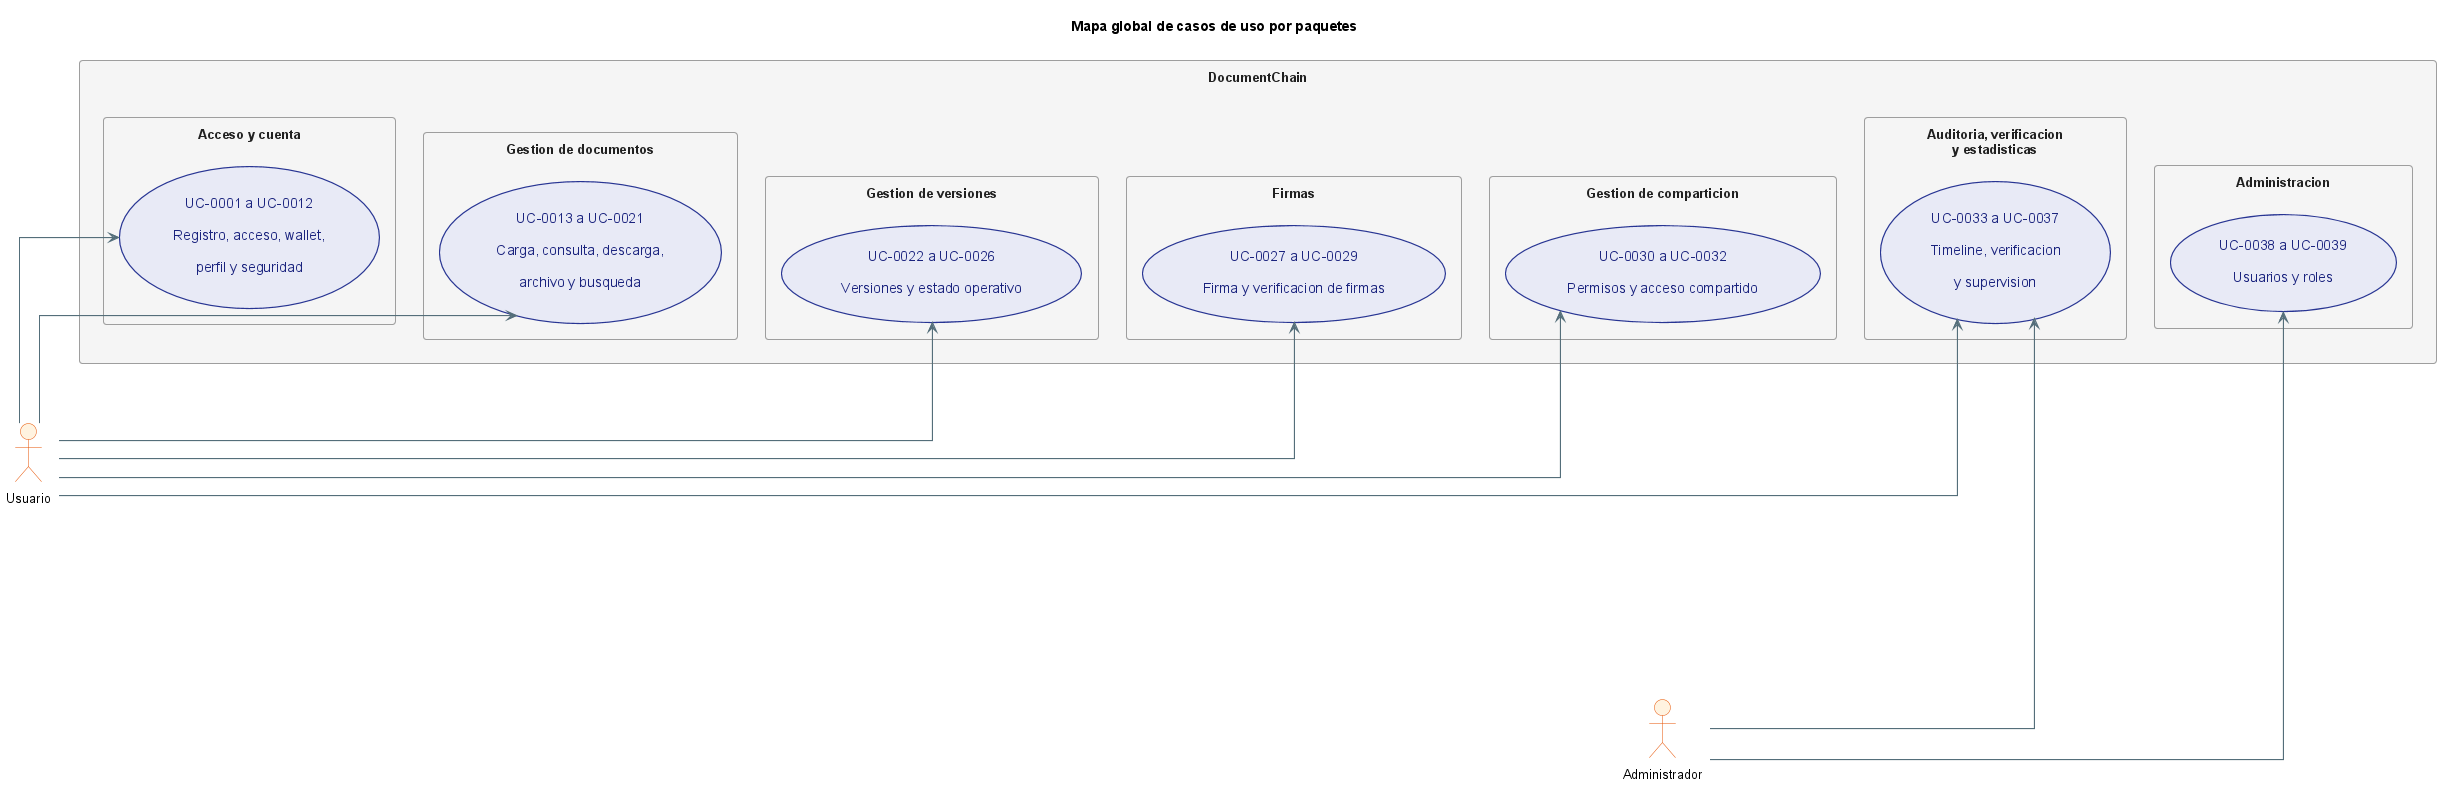
\includegraphics[width=0.92\textwidth]{diagramas/usecase-general.png}
    \caption{Visión general de los casos de uso principales del sistema}
    \label{fig:usecase-general}
\end{figure}

\section{Antecedentes y contexto tecnológico}

La gestión documental es un dominio maduro desde el punto de vista software. Existen soluciones sobradamente capaces para almacenar, clasificar y recuperar archivos, tanto en entornos corporativos como de usuario final. No obstante, el interés de este proyecto no reside en reimplementar un repositorio de documentos genérico, sino en abordar una zona menos atendida por las plataformas convencionales: la evidencia de integridad y de autoría cuando se requiere contrastación más allá del propio proveedor.

\subsection{Sistemas documentales tradicionales}

Los sistemas centralizados resuelven bien la consulta, la indexación y la gestión interna de estados. Su principal ventaja es operativa: permiten búsquedas complejas, bajo tiempo de respuesta y evolución ágil del modelo de datos. El inconveniente aparece cuando se desea separar el estado operativo de la prueba de que una acción ocurrió realmente. Si una firma, un cambio de permiso o una sustitución de versión solo viven en la base de datos interna, la validez de esa evidencia termina siendo indistinguible de la confianza depositada en el administrador del sistema.

Entre las plataformas más representativas del mercado se encuentran soluciones como SharePoint y OneDrive de Microsoft, Google Drive, Alfresco y Liferay en el ámbito empresarial, y DocuSign, Adobe Acrobat Sign o Signaturit en el segmento de firma electrónica. Cada una de ellas responde bien a una parte del problema documental: SharePoint y Google Drive ofrecen versionado y colaboración sobre documentos de oficina; Alfresco aporta gestión de contenido empresarial con flujos de aprobación; DocuSign y similares resuelven la firma electrónica con valor legal mediante infraestructura PKI propia. Sin embargo, ninguna de ellas ofrece de forma nativa la combinación de ciclo de vida completo, firma asociada a dirección blockchain, almacenamiento por contenido vía IPFS y verificación pública contrastable sin autenticación.

La razón no es que estas plataformas sean incompletas, sino que responden a un modelo de confianza diferente. En ese modelo, la autoridad del proveedor es suficiente garantía. Cuando el contexto exige separar la operativa de la evidencia o cuando se quiere que una tercera parte pueda verificar la integridad de forma autónoma, ese modelo encuentra su límite natural.

\subsection{Blockchain como capa de evidencia}

Blockchain resulta pertinente cuando interesa conservar eventos poco ambiguos, de bajo volumen y con valor probatorio. El proyecto adopta esta tecnología no como contenedor general de documentos, sino como registro de creación, versionado, firmas, cambios de titularidad y permisos efectivos. Ese uso restringido es coherente con el coste y la rigidez del entorno \textit{on-chain} y permite extraer valor sin trasladar a la cadena información que debería permanecer fuera de ella.

En el panorama reciente se han desarrollado varios enfoques para aprovechar blockchain en gestión documental. Proyectos como Docusign Blockchain, experimentos con NFT como certificados de propiedad y sistemas de notarización on-chain como OpenTimestamps han explorado distintas formas de anclar documentos a la cadena. Su cobertura funcional, sin embargo, rara vez va más allá del registro del hash inicial: la compartición, el versionado, la firma con identidad pseudónima y la revocación de permisos quedan fuera del alcance del componente blockchain y se gestionan en capas separadas que no siempre se integran con coherencia. DocumentChain cubre ese espacio con un contrato único que coordina todas las operaciones documentales relevantes y las expone como eventos auditables.

\subsection{IPFS y almacenamiento por contenido}

La incorporación de IPFS responde a una necesidad distinta. Cuando el archivo no debe residir únicamente en el backend, el direccionamiento por contenido aporta una forma clara de vincular el binario con un identificador estable derivado de su propio contenido. Esa propiedad encaja de forma natural con el versionado: cada modificación relevante genera un CID diferente y, por tanto, una referencia inequívoca a la versión concreta del documento almacenado.

\subsection{Criptografía aplicada a la gestión documental}

Un sistema con trazabilidad fuerte no puede sacrificar privacidad por el camino. Por ello se incorporan mecanismos de cifrado autenticado para el documento privado, endurecimiento de contraseñas con Argon2id y protección asimétrica de claves simétricas fuera de la cadena. El interés técnico del proyecto se encuentra precisamente en la combinación de estos mecanismos con la operativa normal del usuario, no en la adopción aislada de cada uno de ellos.

\subsection{Justificación del enfoque híbrido}

La combinación PostgreSQL--IPFS--blockchain no se plantea como suma ornamental de tecnologías. Se adopta porque cada componente resuelve una parte concreta del problema y porque el reparto evita dos extremos poco satisfactorios: una plataforma puramente centralizada que no aporta verificabilidad externa y una plataforma puramente on-chain que sería costosa, rígida y poco adecuada para la gestión documental cotidiana.

\section{Descripción de la situación actual}

\subsection{Panorama general de la gestión documental digital}

La gestión documental contemporánea se mueve entre dos necesidades que no siempre se resuelven al mismo tiempo. La primera es eminentemente operativa: almacenar, clasificar, compartir y recuperar documentos de forma rápida. La segunda es de confianza: demostrar quién hizo qué, sobre qué versión y en qué momento. La mayor parte de las plataformas del mercado resuelven con solvencia la primera necesidad, pero solo cubren parcialmente la segunda cuando la verificación debe salir del perímetro del propio sistema.

Entre las plataformas más representativas se encuentran soluciones como Google Drive o Dropbox, que aceleran el almacenamiento y la compartición pero carecen de versionado con evidencia externa. Microsoft 365 y SharePoint ofrecen historial y flujos de aprobación dentro del ecosistema Microsoft, aunque la trazabilidad sigue siendo interna. Plataformas de firma como DocuSign o Adobe Sign proveen mecanismos PKI válidos para firmas electrónicas avanzadas, pero no abordan el ciclo de vida documental completo ni la verificabilidad pública sin cuentas de terceros. También existen plataformas de gestión de contenido empresarial como Alfresco o Nuxeo con capacidades más amplias, pero orientadas a grandes implantaciones y alejadas de la verificabilidad basada en blockchain.

En ese panorama predominan soluciones centralizadas orientadas a productividad y colaboración, muy adecuadas para el trabajo diario, aunque menos expresivas cuando se exige una trazabilidad fuerte y contrastable. También existen plataformas especializadas en firma electrónica o en custodia documental, pero suelen centrarse en etapas concretas del ciclo de vida y no necesariamente en la convivencia entre versionado, compartición, evidencias técnicas y publicación pública controlada.

\subsection{Limitaciones habituales de las soluciones existentes}

Al analizar el estado actual del dominio aparecen varias limitaciones recurrentes. En primer lugar, la evidencia de integridad suele quedar integrada en la misma infraestructura que el resto del estado operativo. En segundo lugar, el modelo de permisos acostumbra a ser suficientemente útil para la colaboración ordinaria, pero no siempre queda respaldado por una huella externa verificable. En tercer lugar, el almacenamiento del binario y la historia de cambios se mantienen bajo la misma autoridad técnica, lo que dificulta separar servicio de confianza.

Estas limitaciones no invalidan a los sistemas centralizados, pero sí acotan el tipo de garantía que pueden ofrecer. Un proveedor puede asegurar que conserva histórico, versiones o firmas, aunque esa afirmación sigue descansando en la autoridad del propio proveedor y en sus mecanismos internos de auditoría. El problema técnico que aborda DocumentChain aparece cuando se quiere complementar esa autoridad con una evidencia externa y contrastable para las operaciones más sensibles.

\begin{table}[H]
    \centering
    \small
    \begin{tabular}{|p{4.4cm}|p{4cm}|p{4.5cm}|}
    \hline
    \textbf{Aspecto} & \textbf{Solución documental convencional} & \textbf{Necesidad identificada en el proyecto} \\
    \hline
    Estado de versiones & Histórico interno gestionado por la plataforma & Huella verificable de creación, sustitución y restauración de versión. \\
    \hline
    Control de acceso & Permisos operativos dentro de la aplicación & Evidencia adicional de titularidad y cambios relevantes de permisos. \\
    \hline
    Firma o conformidad & Registro interno o integración con terceros & Firma asociada a wallet y registro contrastable de la aceptación. \\
    \hline
    Publicación de documentos & Enlaces de compartición bajo control del proveedor & Diferenciación explícita entre contenido privado y contenido público verificable. \\
    \hline
    Auditoría & Dependiente del repositorio central & Posibilidad de contraste externo para los eventos más críticos. \\
    \hline
    \end{tabular}
    \caption{Brecha entre necesidades del dominio y soluciones documentales convencionales}
    \label{tab:brecha-soluciones}
\end{table}

\subsection{Necesidades concretas del proyecto}

El sistema propuesto necesita responder a un conjunto de exigencias que, combinadas, vuelven insuficiente una aproximación puramente monolítica o puramente on-chain. Se requiere autenticación tradicional usable, colaboración documental con distintos niveles de acceso, soporte de documentos privados y públicos, versionado completo, firma con wallet, notificaciones, administración y trazabilidad fuerte. Cada una de estas necesidades podría resolverse de forma aislada con soluciones tecnológicas diferentes, pero el interés del proyecto está en integrarlas de manera coherente dentro de una sola plataforma.

También resulta importante que la solución sea viable en un contexto académico. Eso implica evitar dependencias prohibitivas, reducir barreras de despliegue, reutilizar herramientas con buena documentación y mantener un entorno que pueda ejecutarse localmente. La situación actual del proyecto se entiende mejor desde esa doble exigencia: por un lado, construir una solución técnicamente interesante; por otro, hacerlo con un coste y una complejidad asumibles para un TFG individual.

\section{Normas y referencias}

\subsection{Métodos de desarrollo}

El proyecto se ha conducido con una lógica iterativa e incremental inspirada en el Proceso Unificado. Esta elección resulta coherente con un sistema en el que conviven componentes de naturaleza muy distinta, como una SPA en React, un backend transaccional, un contrato inteligente y un subsistema de almacenamiento distribuido. Un desarrollo estrictamente lineal habría dificultado la detección temprana de incompatibilidades entre capas; en cambio, la organización por fases e iteraciones ha permitido estabilizar antes la arquitectura, validar hipótesis de integración y reducir el riesgo técnico en los componentes más novedosos.

La estimación del esfuerzo se ha apoyado en puntos de caso de uso ajustados, tal como se desarrolla en el Anexo III. Esta referencia metodológica no se ha utilizado únicamente para obtener una cifra global de horas, sino también para ordenar el proyecto por bloques funcionales y priorizar primero las piezas sin las cuales el sistema no tendría recorrido defendible: autenticación, ciclo documental, integración blockchain, cifrado, compartición y validación. Sobre esa base se incorporaron después paneles administrativos, notificaciones, exploración de eventos y mejoras de operación.

\subsection{Herramientas de ingeniería y soporte}

El desarrollo del sistema se ha apoyado en un conjunto de herramientas seleccionadas por su madurez, compatibilidad entre capas y adecuación al contexto académico del proyecto. En la Tabla~\ref{tab:herramientas-referencia} se recoge un resumen por ámbito; a continuación se describe cada herramienta con mayor detalle.

\begin{table}[H]
    \centering
    \small
    \begin{tabular}{|p{2.8cm}|p{3.6cm}|p{6.6cm}|}
    \hline
    \textbf{Ámbito} & \textbf{Herramientas principales} & \textbf{Finalidad dentro del proyecto} \\
    \hline
    Frontend & React, Vite, TypeScript, Tailwind CSS & Construcción de la SPA, tipado fuerte, organización de rutas y experiencia de usuario. \\
    \hline
    Backend & Node.js, Express, Prisma, Zod & API REST, validación de entrada, lógica de negocio y acceso a PostgreSQL. \\
    \hline
    Blockchain & Solidity, Hardhat, Ethers, OpenZeppelin & Desarrollo, despliegue local y validación del contrato \texttt{DocumentRegistry}. \\
    \hline
    Persistencia y operación & PostgreSQL, IPFS, Docker Compose, Nginx, Postfix & Almacenamiento, integración de servicios, publicación del frontend y salida SMTP. \\
    \hline
    Pruebas y documentación & Jest, Playwright, LaTeX, PlantUML, EZEstimate & Validación automatizada, elaboración de diagramas, redacción académica y estimación. \\
    \hline
    \end{tabular}
    \caption{Herramientas de referencia empleadas en el desarrollo de DocumentChain}
    \label{tab:herramientas-referencia}
\end{table}

\subsubsection{React, Vite y TypeScript}

React es la biblioteca de interfaz de usuario más extendida en el ecosistema JavaScript. Su modelo de componentes declarativos facilita la organización de la interfaz en piezas independientes con estado propio, algo especialmente conveniente en una plataforma documental con vistas complejas, flujos de datos asíncronos y múltiples modales de acción. La combinación con Vite, un empaquetador de nueva generación basado en ESBuild y Rollup, reduce los tiempos de recompilación en desarrollo a escala de milisegundos y genera un \textit{bundle} de producción optimizado.

El uso de TypeScript introduce tipado estático que permite detectar inconsistencias antes de la ejecución. En un sistema con múltiples entidades de dominio, permisos diferenciados, respuestas de API y operaciones críticas en blockchain, contar con tipos explícitos para documentos, versiones, firmas y acciones de usuario tiene valor práctico durante el desarrollo e incrementa la confianza al refactorizar. La Figura~\ref{fig:login-page-herramienta} muestra la pantalla de inicio de sesión, ilustración del resultado final de esta capa de presentación.

\begin{figure}[H]
    \centering
    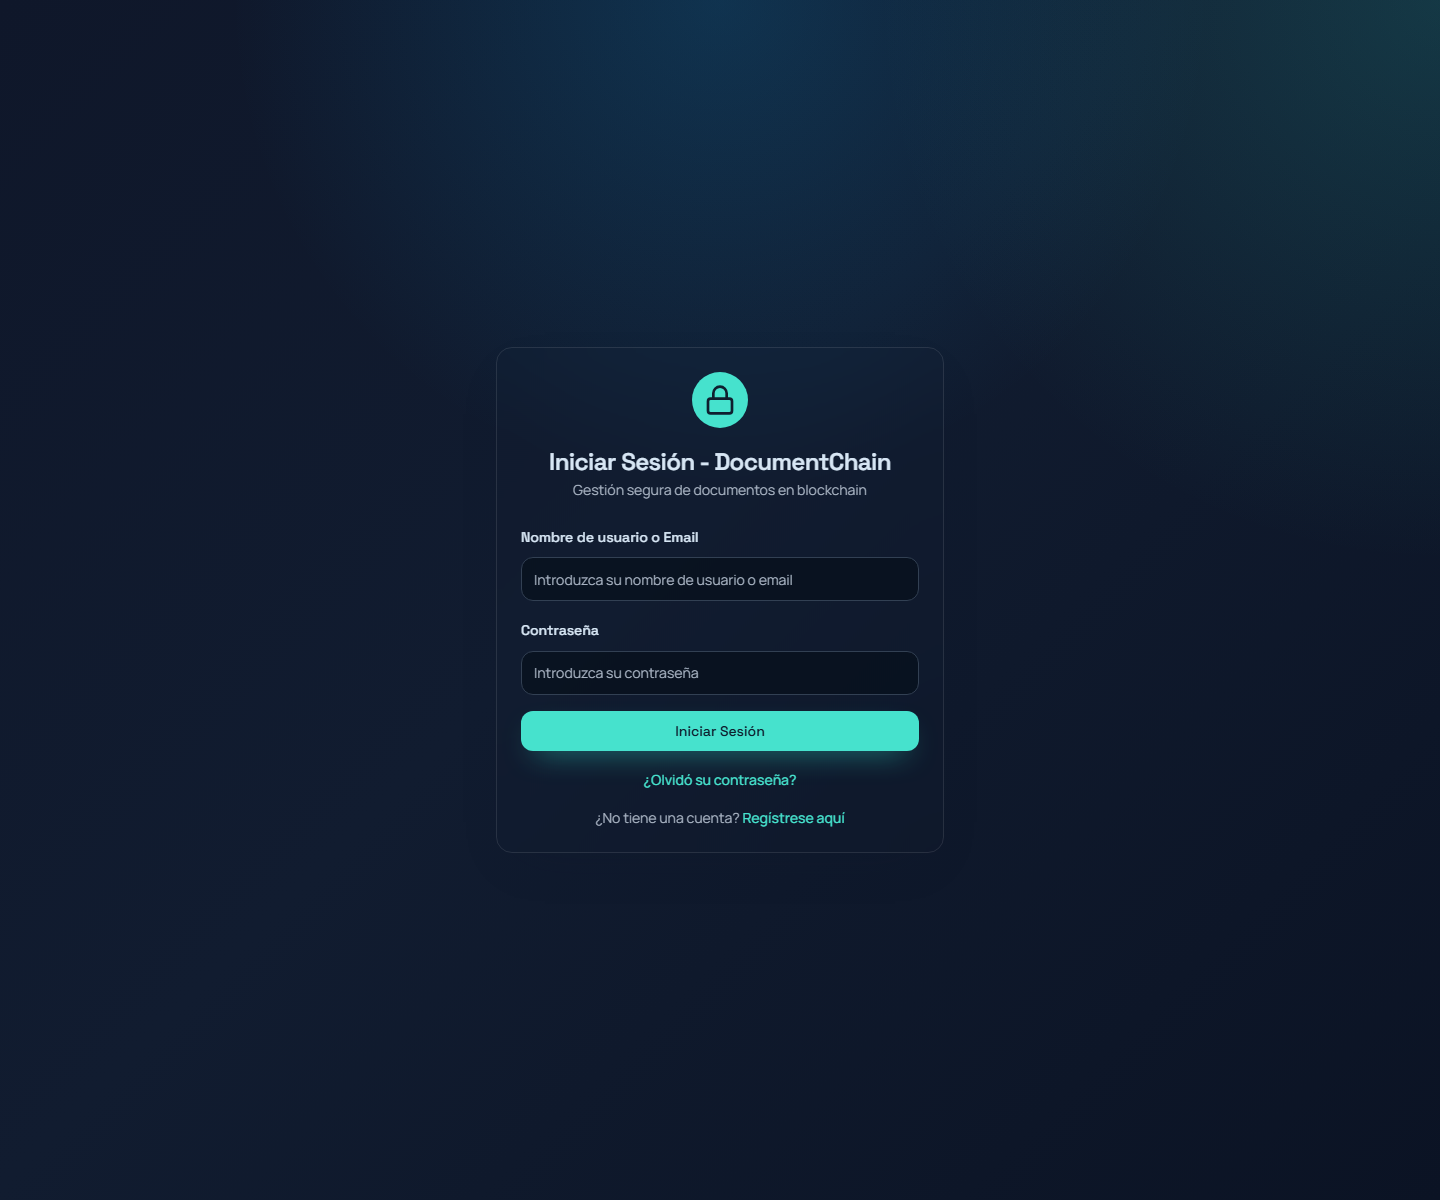
\includegraphics[width=0.88\textwidth]{capturas-ui/login-page.png}
    \caption{Vista de inicio de sesión construida con React, Vite y TypeScript}
    \label{fig:login-page-herramienta}
\end{figure}

\subsubsection{Node.js y Express}

Node.js proporciona el entorno de ejecución para el backend. Su bucle de eventos orientado a entrada/salida no bloqueante resulta adecuado para una API que combina consultas a PostgreSQL, cifrado de binarios, subidas a IPFS y coordinación con el nodo Hardhat. La elección tiene también la ventaja de mantener TypeScript en ambos extremos del stack, reduciendo así la barrera mental entre los modelos de datos del frontend y del backend.

Express se adopta como marco ligero para la API REST. Ofrece enrutado claro, facilidad para organizar middlewares de autenticación, validación y manejo de errores, y un ecosistema amplio de módulos. Su deliberada ausencia de estructura rígida exige una organización explícita, que el proyecto resuelve separando controladores, servicios, configuración y utilidades en capas diferenciadas. El siguiente fragmento ilustra el patrón de validación empleado en los \textit{endpoints}:

\begin{lstlisting}[language=JavaScript, caption={Fragmento representativo de un controlador Express en DocumentChain}]
router.post('/documents', authenticate, async (req, res) => {
  const parsed = CreateDocumentSchema.safeParse(req.body);
  if (!parsed.success)
    return res.status(400).json({ error: parsed.error });
  const doc = await documentService.create(req.user.id, parsed.data);
  return res.status(201).json(doc);
});
\end{lstlisting}

\subsubsection{Prisma}

Prisma actúa como capa de acceso a datos entre el backend y PostgreSQL. Su esquema declarativo en \texttt{schema.prisma} permite definir el modelo relacional de forma legible, generar migraciones reproducibles y obtener tipos TypeScript derivados automáticamente del esquema. Esta propiedad resulta especialmente valiosa cuando el modelo de datos cambia durante el desarrollo: el compilador detecta de inmediato las consultas que no son coherentes con los tipos actualizados. Prisma también reduce la probabilidad de inyecciones SQL al gestionar el escape de parámetros internamente.

\subsubsection{PostgreSQL}

PostgreSQL es la base de datos elegida para el estado operativo del sistema. Su solidez como motor relacional, su soporte nativo para tipos JSON cuando conviene, su integración con Prisma y su compatibilidad con el despliegue dockerizado lo convierten en la alternativa más natural para el contexto del proyecto. El esquema mantiene tablas explícitas para usuarios, wallets, documentos, versiones, firmas sincronizadas, notificaciones y carpetas. La Figura~\ref{fig:er-diagram-herramienta} muestra el modelo entidad-relación.

\begin{figure}[H]
    \centering
    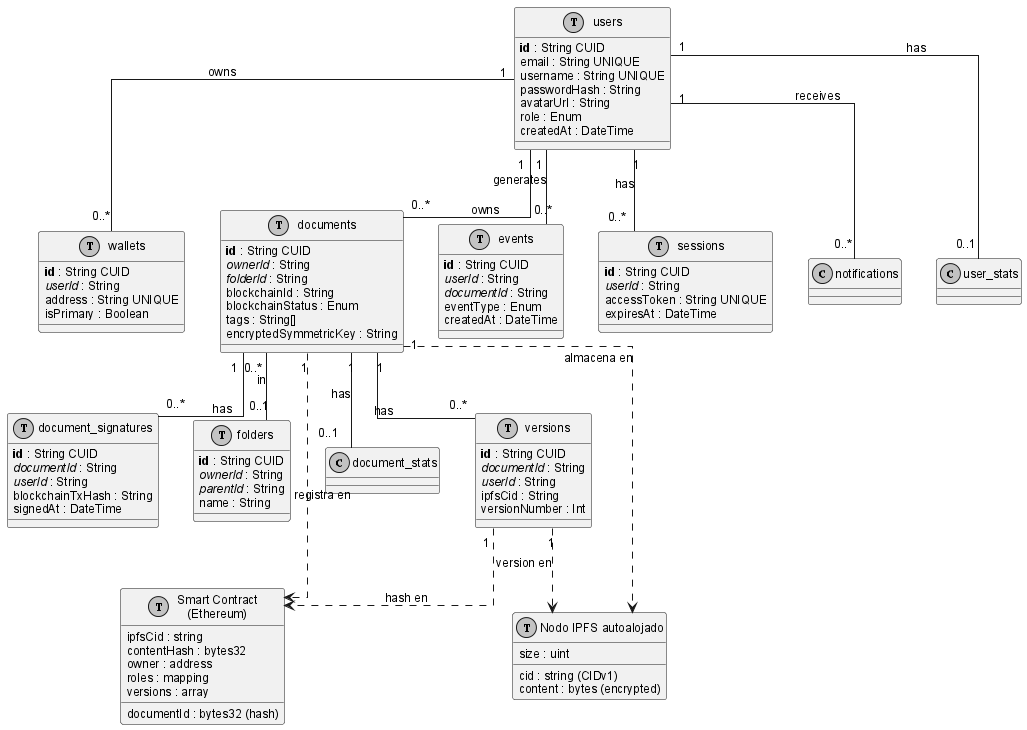
\includegraphics[width=0.97\textwidth]{diagramas/er-diagram.png}
    \caption{Modelo entidad-relación del esquema operativo gestionado por Prisma sobre PostgreSQL}
    \label{fig:er-diagram-herramienta}
\end{figure}

\subsubsection{Solidity y Hardhat}

El contrato inteligente del sistema se ha escrito en Solidity, el lenguaje de referencia para la EVM (\textit{Ethereum Virtual Machine}). La elección se apoya en su madurez, en la disponibilidad de librerías de seguridad como OpenZeppelin y en la compatibilidad directa con Hardhat. El contrato \texttt{DocumentRegistry} concentra la lógica de registro documental, versionado, firmas, permisos y pausa de emergencia en un único artefacto, lo que simplifica la correlación entre operación de negocio y evento emitido. A continuación se muestra la estructura principal del contrato:

\begin{lstlisting}[language=C, caption={Estructura del contrato DocumentRegistry en Solidity}]
contract DocumentRegistry is Ownable, Pausable {
    struct Document {
        address owner;
        uint256 currentVersion;
        bool archived;
        bool deleted;
    }
    struct Version {
        uint256 number;
        string cid;
        address author;
        bool isActive;
    }
    mapping(bytes32 => Document) public documents;
    event DocumentRegistered(bytes32 indexed docId, address owner);
    event VersionAdded(bytes32 indexed docId, uint256 version, string cid);
}
\end{lstlisting}

Hardhat es el entorno de desarrollo y prueba utilizado para desplegar la red local Ethereum, ejecutar el contrato con determinismo total y lanzar las pruebas con Mocha. Proporciona un ciclo de desarrollo completamente reproducible, lo que facilita la demostración del comportamiento \textit{on-chain} en cualquier máquina sin depender de una red pública.

\subsubsection{Ethers y OpenZeppelin}

Ethers.js es la librería JavaScript que conecta el frontend con el nodo Ethereum. Gestiona la codificación ABI, el envío de transacciones, la escucha de eventos y la consulta de estados del contrato desde el navegador. En combinación con MetaMask, permite que el usuario autorice operaciones críticas desde su propia wallet sin que la clave privada salga del entorno del cliente.

OpenZeppelin aporta implementaciones auditadas de patrones de seguridad para contratos inteligentes: \texttt{Ownable} para la gestión del propietario del contrato, \texttt{Pausable} para el mecanismo de pausa de emergencia y utilidades de control de acceso que reducen la probabilidad de vulnerabilidades habituales en contratos Solidity.

\subsubsection{IPFS}

IPFS (\textit{InterPlanetary File System}) es una red de almacenamiento distribuido cuyos contenidos se identifican por su propio hash criptográfico, el CID (\textit{Content Identifier}). Su incorporación al proyecto responde a una necesidad concreta: separar el binario del documento del backend de la aplicación y permitir que la referencia al contenido sea estable e independiente de la infraestructura del proveedor.

La integración se ha diseñado alrededor de un nodo Kubo autoalojado expuesto por API HTTP. Cada documento y cada versión generan un CID único que se registra tanto en PostgreSQL como en blockchain, creando la vinculación entre contenido, evidencia y trazabilidad que da sentido a la arquitectura híbrida del proyecto.

\subsubsection{Docker Compose}

Docker Compose es la herramienta de orquestación que coordina los servicios del sistema en el entorno de desarrollo y en la demostración de entrega. La composición final incluye contenedores para PostgreSQL, Hardhat, el backend, el frontend servido por Nginx y Postfix, cada uno con su configuración de red, volúmenes y variables de entorno. La principal ventaja es la reproducibilidad: el evaluador puede poner en marcha la solución completa con un único comando sin instalar ni configurar manualmente los componentes individuales. La Figura~\ref{fig:deployment-herramienta} muestra la topología resultante.

\begin{figure}[H]
    \centering
    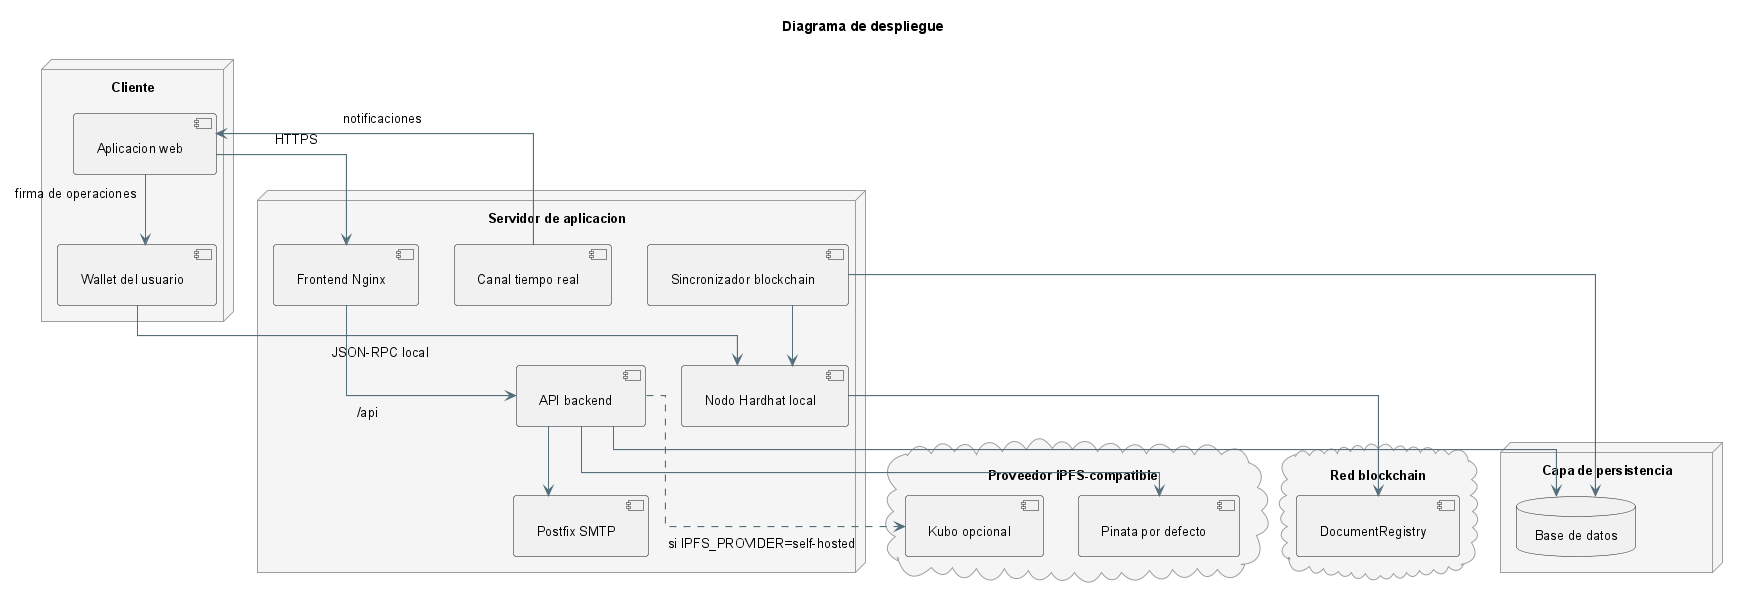
\includegraphics[width=0.92\textwidth]{diagramas/deployment.png}
    \caption{Topología de despliegue mediante Docker Compose con los servicios del sistema}
    \label{fig:deployment-herramienta}
\end{figure}

\subsubsection{Nginx}

Nginx se utiliza como servidor HTTP en el despliegue dockerizado. Publica el \textit{build} estático generado por Vite, gestiona el enrutado interno de la SPA redirigiendo cualquier ruta no reconocida al \texttt{index.html} y, cuando la configuración lo requiere, actúa como proxy inverso canalizando las peticiones API del frontend hacia el servicio de backend. Su ligereza y su amplio soporte de configuración lo convierten en la elección estándar para servir aplicaciones React en producción contenerizada.

\subsubsection{Postfix}

Postfix actúa como servidor SMTP de salida dentro del stack Docker. Su papel es recibir los mensajes generados por el backend, aplicar la configuración de relay autenticado y entregarlos al proveedor de salida configurado. Esta arquitectura desacopla la lógica de generación de correo del proveedor de entrega: el backend no necesita conocer si el correo sale vía Brevo, SendGrid u otro relay. La gestión de plantillas, activaciones, recuperaciones de contraseña y notificaciones de eventos se delega enteramente al backend, mientras Postfix resuelve el transporte.

\subsubsection{Git}

La gestión del código fuente se realiza con Git. El flujo de ramas ha permitido el desarrollo paralelo de frontend, backend, contratos y documentación académica, manteniendo una historia coherente de cambios. El historial del repositorio constituye una fuente de trazabilidad técnica complementaria a los diagramas: recoge en orden cronológico las decisiones de diseño e implementación tomadas a lo largo del proyecto.

\subsubsection{PlantUML}

PlantUML es la herramienta de diagramación textual utilizada para generar diagramas de casos de uso, secuencia, clases, componentes y despliegue. Su enfoque permite mantener los diagramas en control de versiones y regenerarlos de forma reproducible a partir de ficheros \texttt{.puml}. La Figura~\ref{fig:plantuml-ejemplo} muestra el diagrama de secuencia del flujo de subida documental generado con esta herramienta.

\begin{figure}[H]
    \centering
    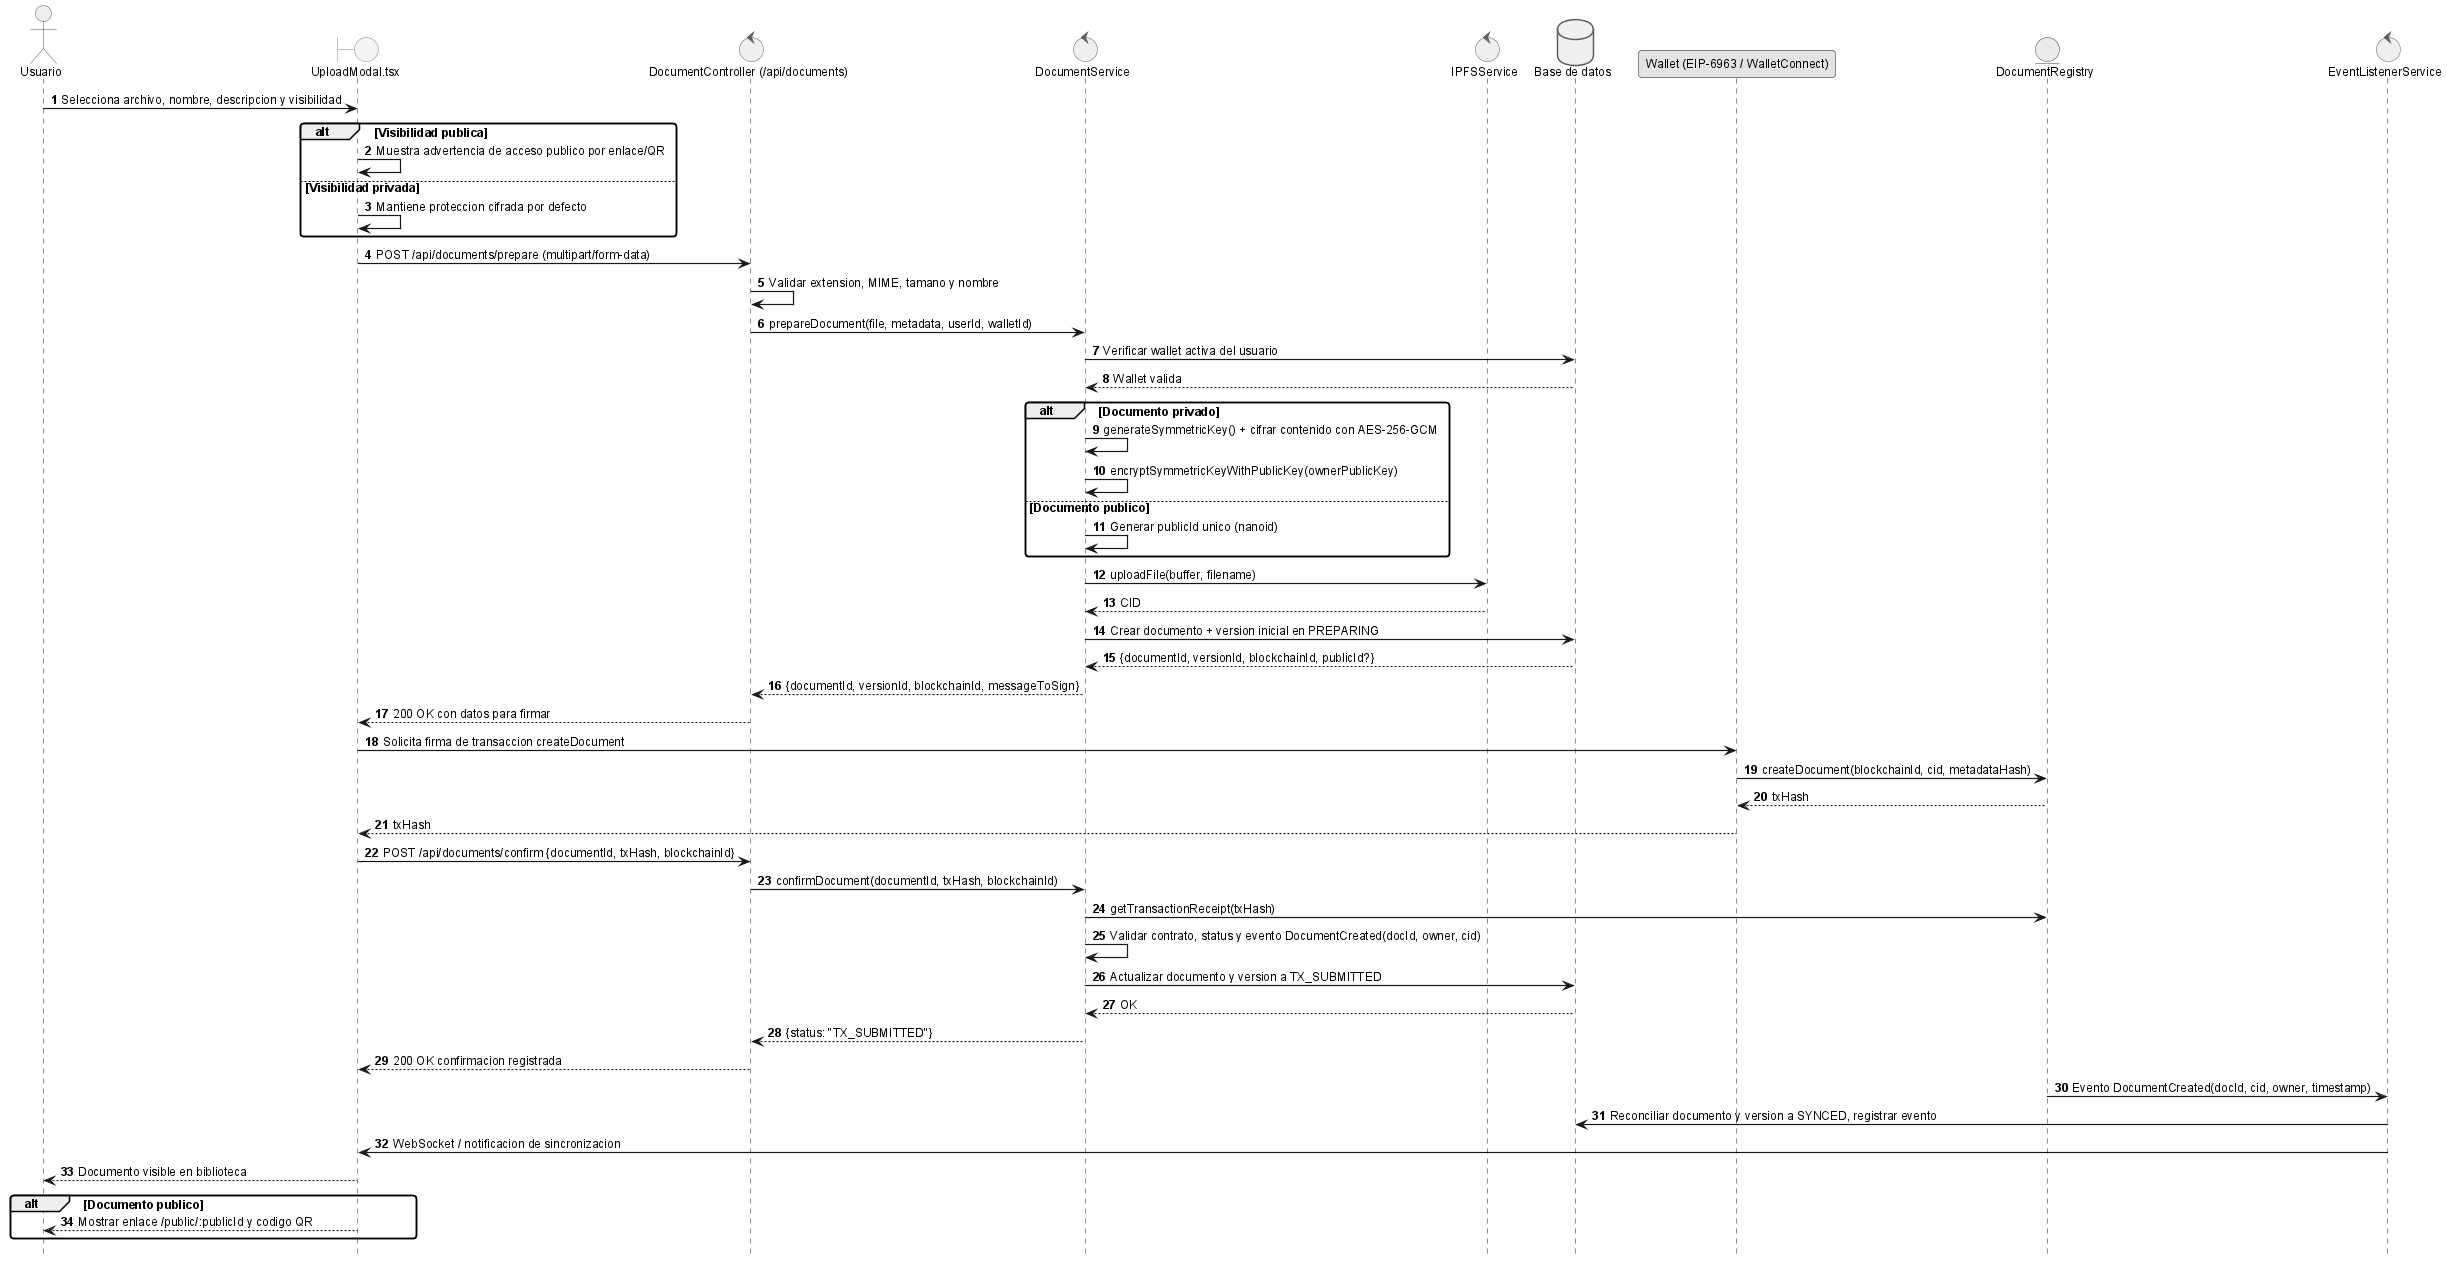
\includegraphics[width=0.88\textwidth]{diagramas/seq-upload.png}
    \caption{Diagrama de secuencia del flujo de subida documental generado con PlantUML}
    \label{fig:plantuml-ejemplo}
\end{figure}

\subsubsection{Jest y Playwright}

La validación automatizada descansa en dos herramientas complementarias. Jest se utiliza para pruebas unitarias e integradas del backend y del contrato inteligente mediante Hardhat. Permite organizar suites, configurar cobertura y ejecutar pruebas en paralelo. Playwright se utiliza para pruebas funcionales del frontend: su capacidad de interactuar con el navegador real, incluida MetaMask cuando la prueba lo requiere, permite automatizar recorridos que van desde el registro hasta la verificación pública, pasando por la firma y la compartición de documentos.

\subsubsection{EZEstimate}

EZEstimate es la herramienta utilizada para calcular el esfuerzo del proyecto a partir de puntos de caso de uso ajustados. A partir de los actores, los casos de uso catalogados y los factores de ajuste técnico y del entorno, produce una estimación de horas que sirve de referencia para la planificación. La Figura~\ref{fig:ezestimate-herramienta} muestra el resultado del cálculo para DocumentChain.

\begin{figure}[H]
    \centering
    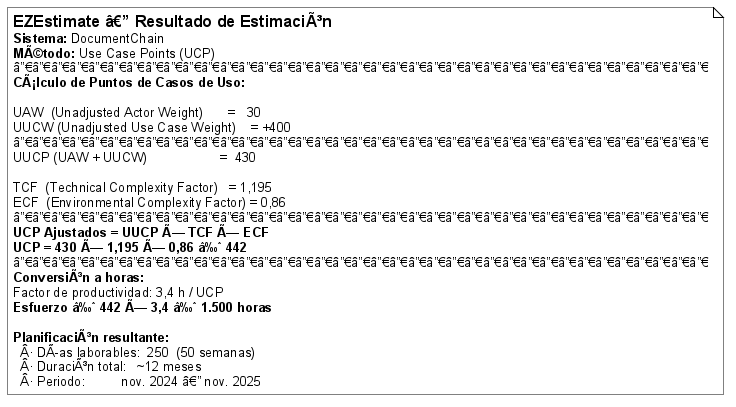
\includegraphics[width=0.84\textwidth]{diagramas/ezestimate.png}
    \caption{Resultado de la estimación UCP del proyecto en EZEstimate}
    \label{fig:ezestimate-herramienta}
\end{figure}

\subsubsection{LaTeX}

La documentación académica del proyecto se ha redactado en \LaTeX{} con la plantilla oficial de la Universidad de Salamanca. La elección frente a procesadores convencionales responde a su capacidad para gestionar documentos extensos con índices, referencias cruzadas, bibliografía y figuras de forma consistente y reproducible. La compilación con LuaHBTeX permite utilizar fuentes OpenType y gestionar correctamente la tipografía española. Cada anexo y la propia memoria se compilan de forma independiente, lo que facilita la revisión parcial e incremental durante el desarrollo del proyecto.

\subsection{Referencias técnicas y normativas}

La memoria y los anexos no se apoyan únicamente en la observación del código, sino también en referencias externas que ayudan a justificar decisiones concretas. Ethereum, Solidity e IPFS proporcionan el marco técnico de la capa de evidencia y almacenamiento distribuido. OpenZeppelin aporta utilidades de seguridad para el contrato inteligente. El RFC de Argon2 sirve de base para el endurecimiento de credenciales. OWASP orienta las decisiones preventivas sobre la API y la interfaz. Y el RGPD junto con la LOPDGDD permiten situar el tratamiento de documentos privados, enlaces públicos y trazabilidad dentro de un marco normativo reconocible.

En consecuencia, la documentación resultante no se limita a describir cómo funciona el sistema, sino también bajo qué criterios se considera aceptable esa solución. Esta distinción es relevante en un TFG, porque un sistema puede ser técnicamente operativo y, sin embargo, estar insuficientemente justificado desde el punto de vista de seguridad, privacidad o mantenibilidad.

\subsection{Prototipos, diagramas y evidencia visual}

La referencia utilizada para orientar esta memoria concede un peso importante a la evolución desde boceto hasta producto validado, incluyendo storyboards de usuario, prototipos de baja fidelidad para cada vista y capturas finales que demuestran la correspondencia entre diseño e implementación. En DocumentChain se ha seguido la misma lógica, adaptada al contexto de una plataforma de gestión documental.

\subsubsection{Storyboards}

Un storyboard captura en secuencia la experiencia de uso de un actor desde su perspectiva narrativa, antes de entrar en el detalle técnico. Para DocumentChain se han definido dos storyboards principales que representan los recorridos de mayor valor desde el punto de vista funcional.

\textbf{Storyboard 1: Alta y firma de un documento por parte del propietario.} El usuario necesita registrar un contrato en la plataforma y dejar constancia de su firma. Accede a la plataforma con sus credenciales, activa su wallet si no lo ha hecho previamente y selecciona la opción de subir documento. Completa el formulario de alta con título, descripción, carpeta (opcional), etiquetas y opción de visibilidad. La plataforma le solicita la firma de la transacción desde MetaMask. Una vez confirmada, el documento aparece en su listado con el CID de IPFS, el hash de la transacción y la opción de consultar la evidencia en el explorador blockchain. Desde el detalle del documento, el usuario accede a la pestaña de firmas y suscribe el documento con su wallet, añadiendo un comentario visible para los usuarios compartidos.

\textbf{Storyboard 2: Verificación pública por parte de un tercero.} Un auditor externo ha recibido por correo un enlace de verificación pública de un documento. Sin necesidad de registro, accede a la URL pública del sistema y visualiza los metadatos del documento, la fecha de alta, el CID y el historial de firmas registrado en blockchain. Puede confirmar por sí mismo que el hash del documento que tiene en local coincide con el CID almacenado. Si el propietario ha habilitado la auditoría pública completa, también puede consultar el historial de versiones y los eventos de permisos registrados en el contrato. El proceso completo no requiere cuenta en la plataforma ni conocimiento técnico de blockchain.

\subsubsection{Bocetos de baja fidelidad}

La fase de diseño de la interfaz comenzó con bocetos de baja fidelidad que establecen la estructura de cada vista antes de entrar en la implementación. Estos bocetos siguen una convención de \textit{wireframe} en escala de grises que prioriza la disposición de elementos sobre el acabado visual. Las once vistas prototipadas cubren los flujos principales del sistema.

La Figura~\ref{fig:wf-login} muestra el boceto de la pantalla de inicio de sesión, punto de entrada principal al sistema.

\begin{figure}[H]
    \centering
    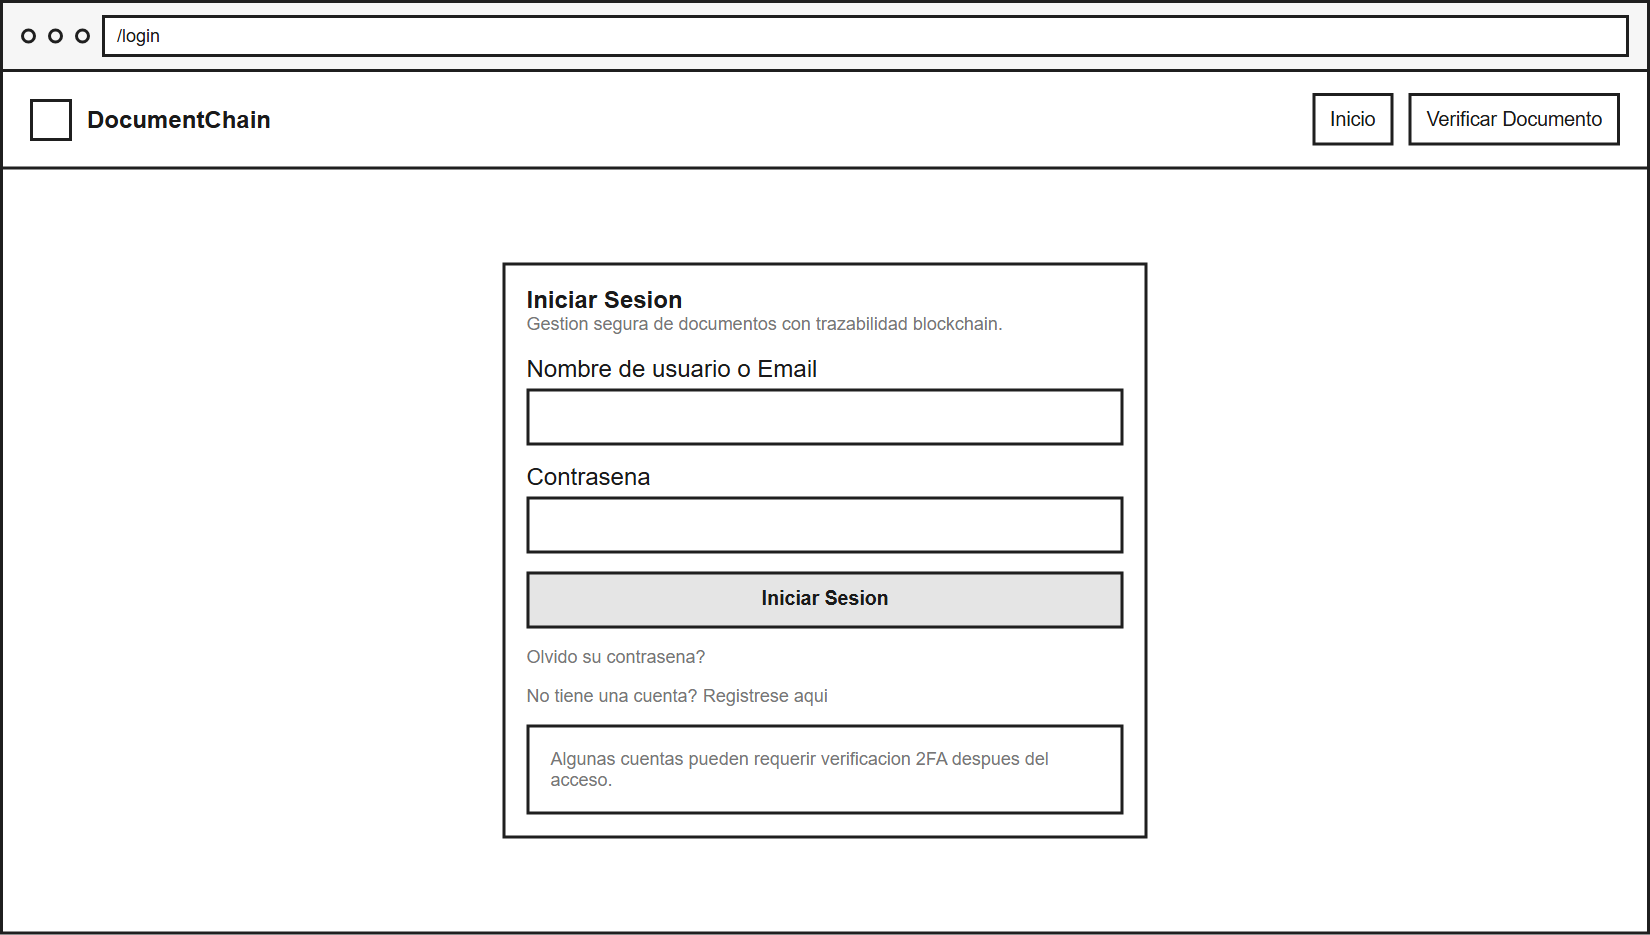
\includegraphics[width=0.82\textwidth]{bocetos-anexo2/login-wireframe.png}
    \caption{Boceto de baja fidelidad de la pantalla de inicio de sesión}
    \label{fig:wf-login}
\end{figure}

La Figura~\ref{fig:wf-register} corresponde al formulario de registro de nuevo usuario.

\begin{figure}[H]
    \centering
    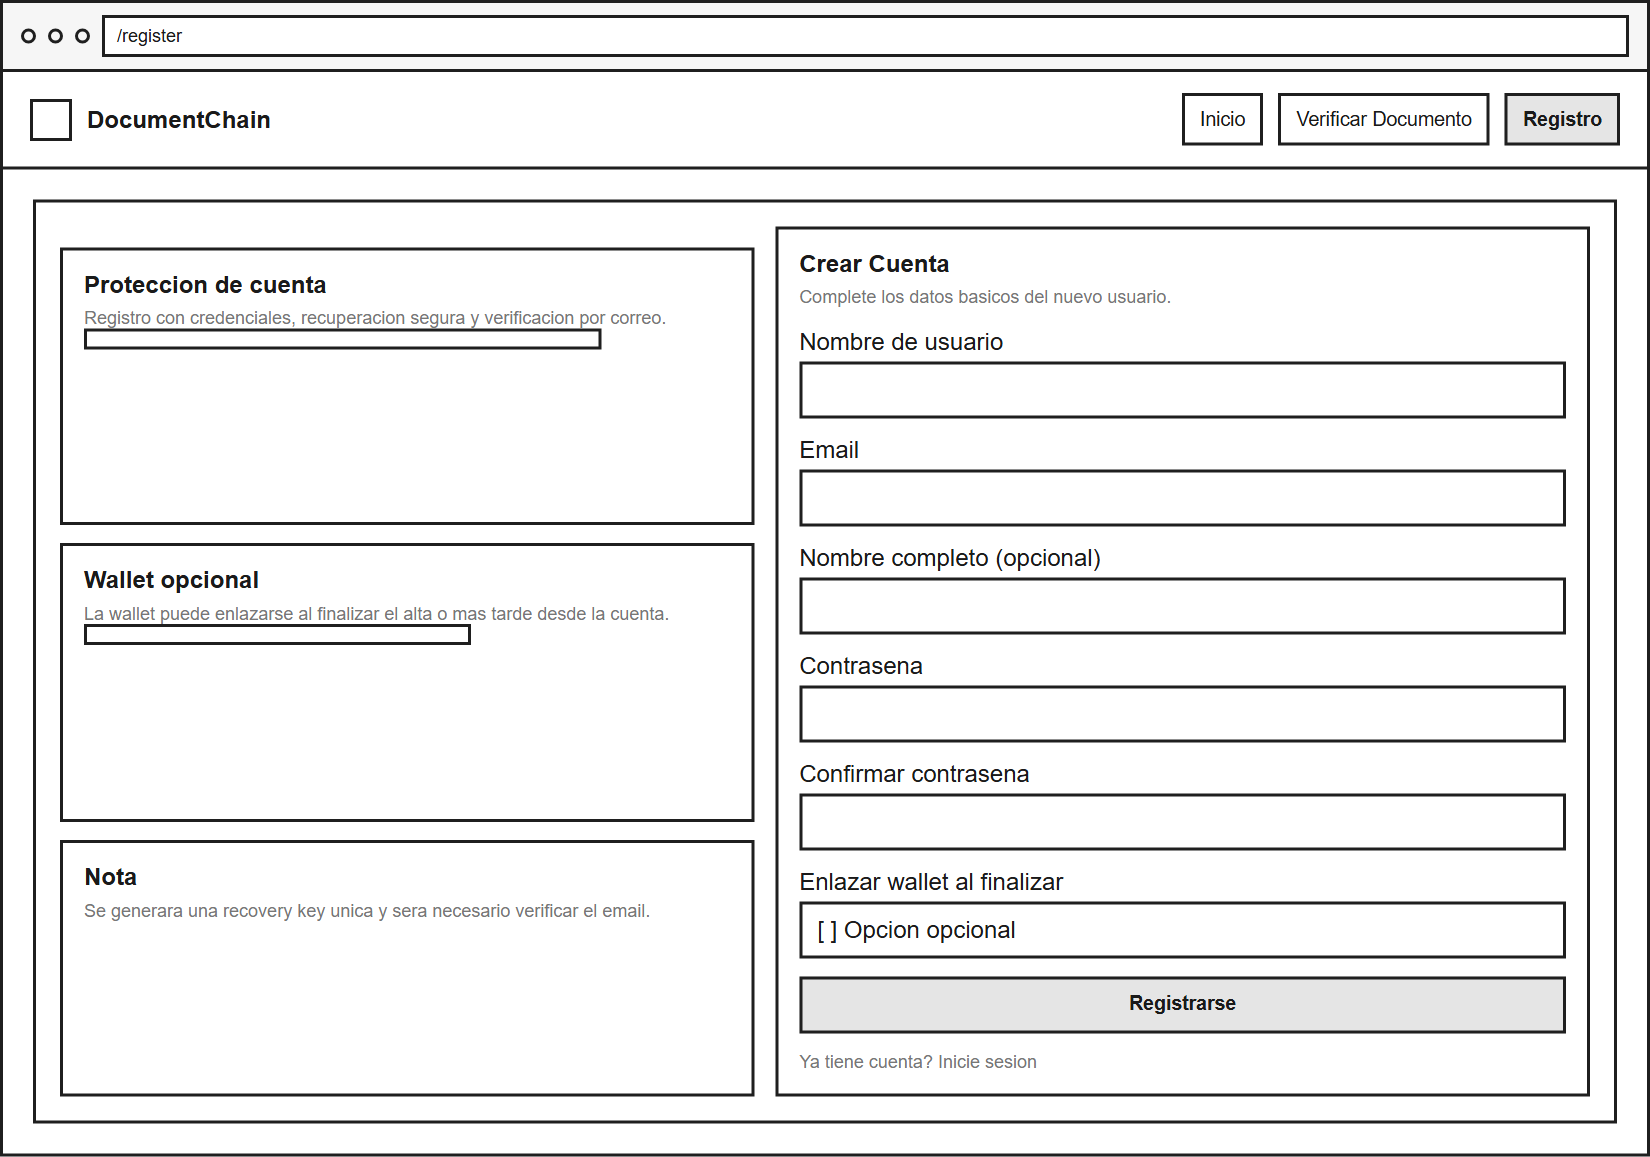
\includegraphics[width=0.82\textwidth]{bocetos-anexo2/register-wireframe.png}
    \caption{Boceto de baja fidelidad del formulario de registro de usuario}
    \label{fig:wf-register}
\end{figure}

La Figura~\ref{fig:wf-documents} muestra el panel principal de gestión documental del usuario autenticado.

\begin{figure}[H]
    \centering
    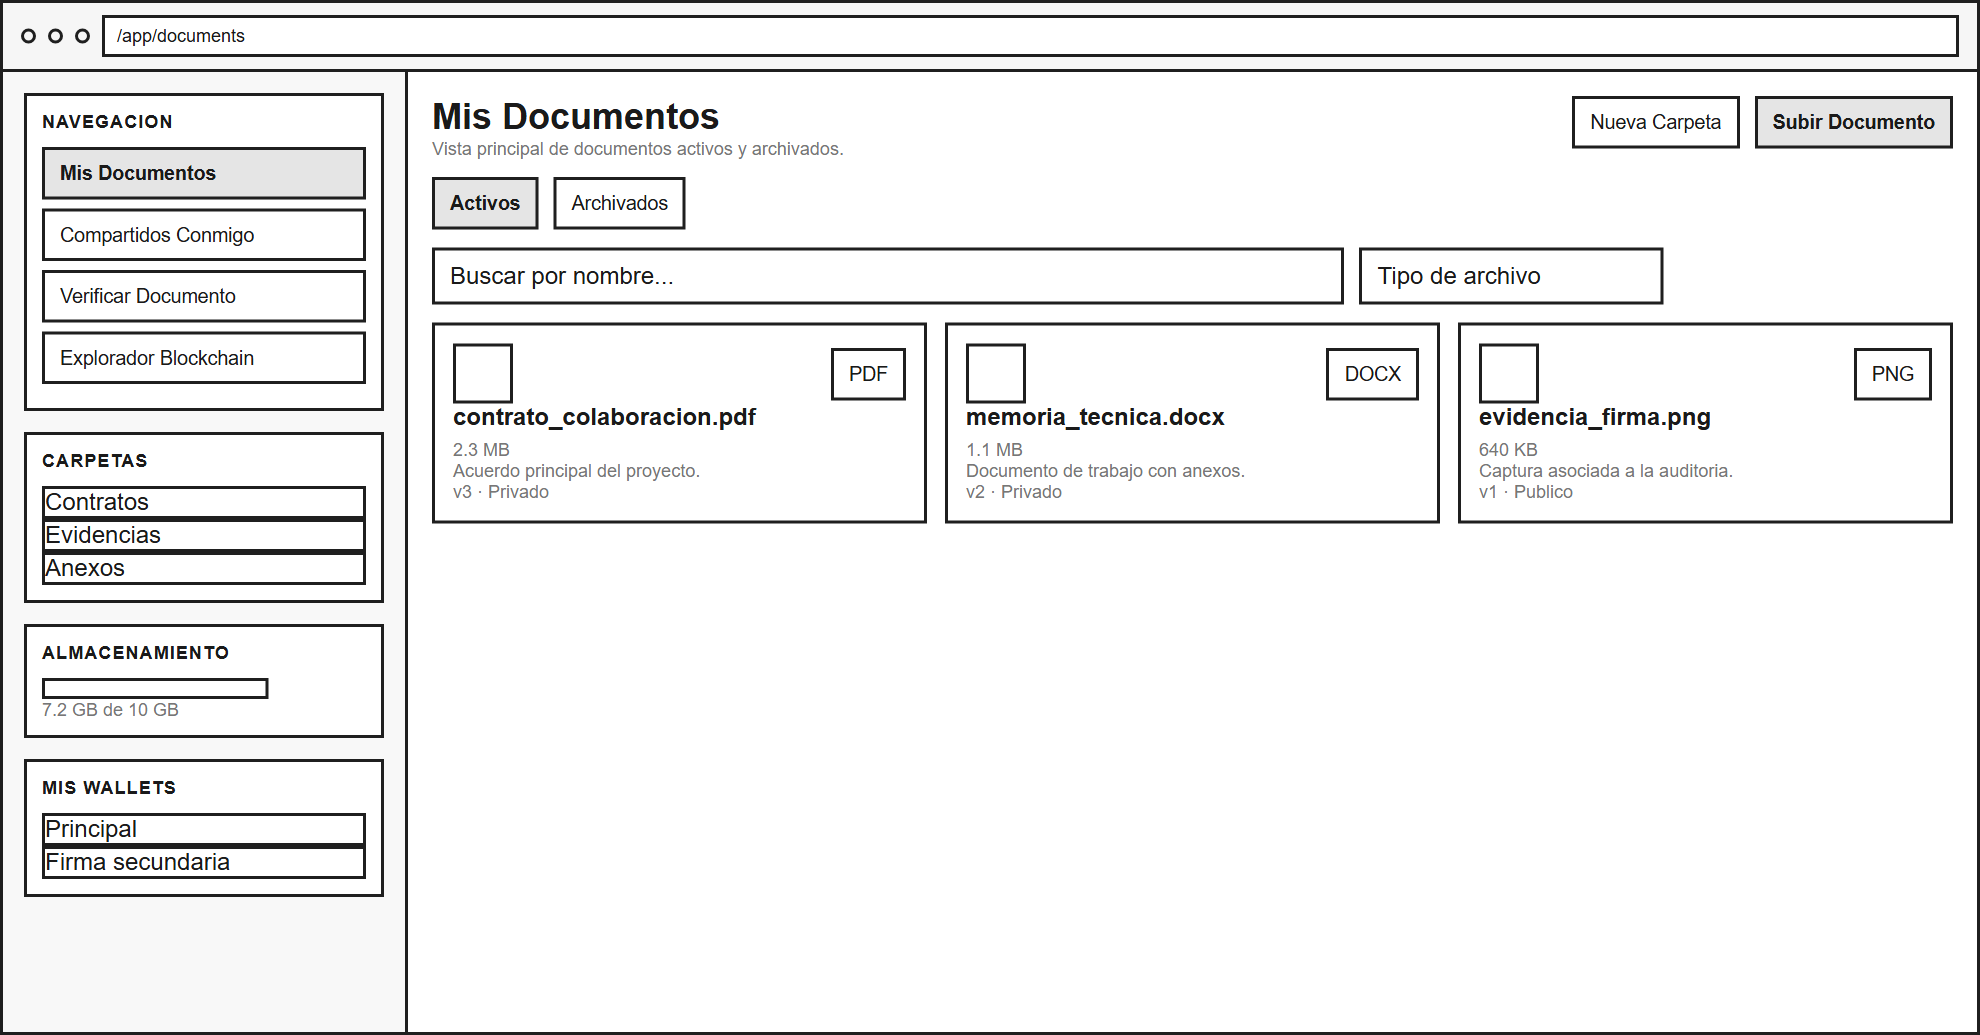
\includegraphics[width=0.87\textwidth]{bocetos-anexo2/documents-dashboard-wireframe.png}
    \caption{Boceto estructural del panel principal de gestión documental}
    \label{fig:wf-documents}
\end{figure}

La Figura~\ref{fig:wf-detail} ilustra la vista de detalle de un documento con sus pestañas operativas.

\begin{figure}[H]
    \centering
    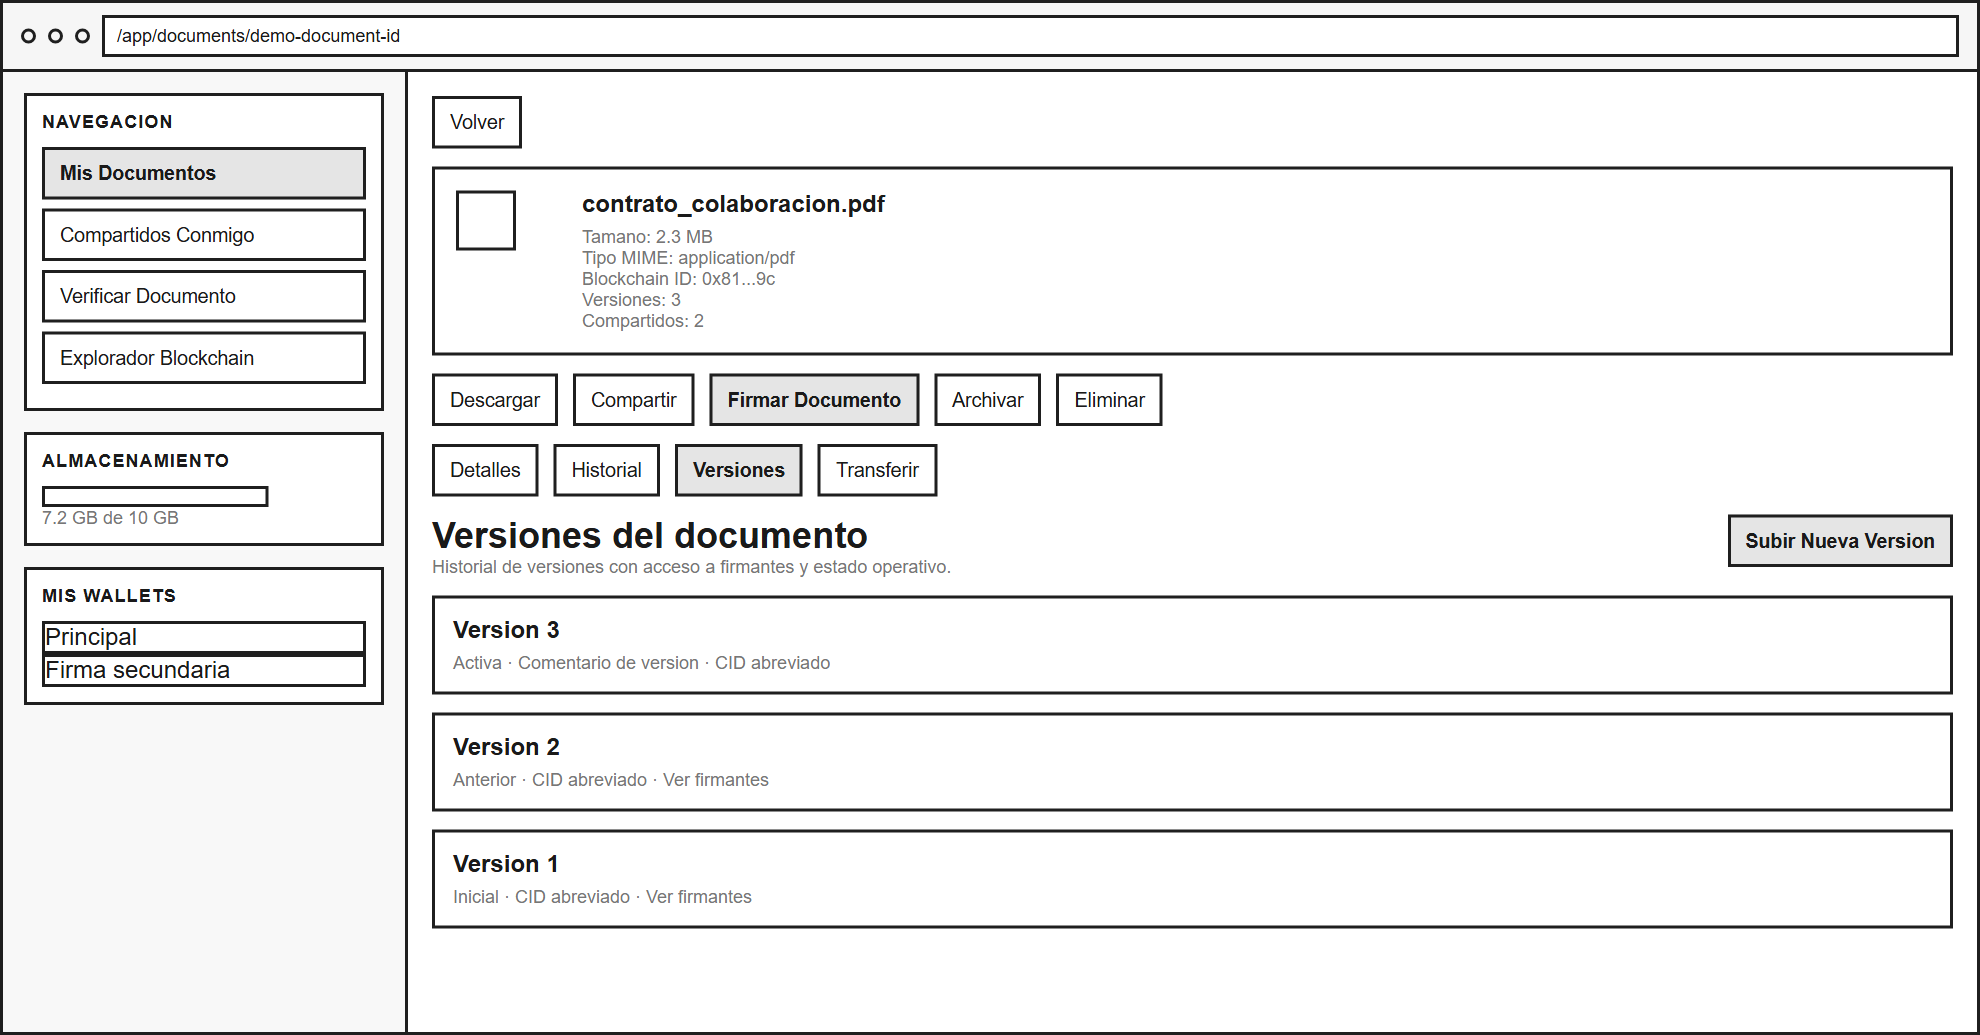
\includegraphics[width=0.87\textwidth]{bocetos-anexo2/document-detail-wireframe.png}
    \caption{Boceto estructural de la vista de detalle documental con pestañas de versiones, firmas y actividad}
    \label{fig:wf-detail}
\end{figure}

La Figura~\ref{fig:wf-share} muestra el diálogo de compartición con selección de usuario y rol.

\begin{figure}[H]
    \centering
    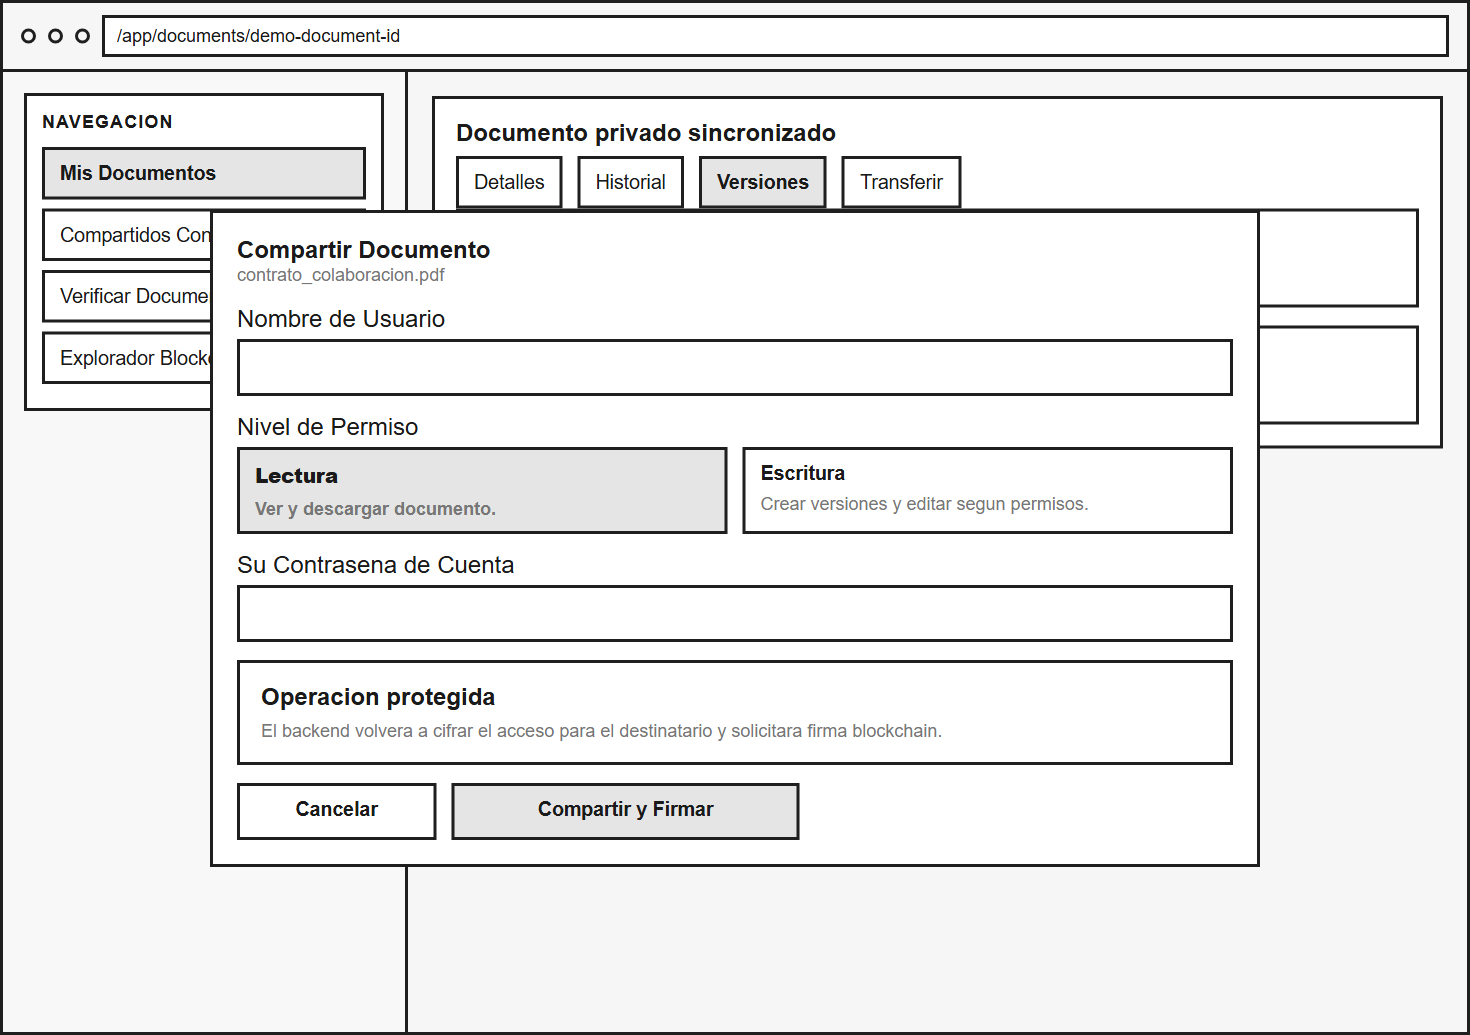
\includegraphics[width=0.75\textwidth]{bocetos-anexo2/share-modal-wireframe.png}
    \caption{Boceto del diálogo de compartición y asignación de roles}
    \label{fig:wf-share}
\end{figure}

La Figura~\ref{fig:wf-shared} muestra la vista de documentos compartidos con el usuario.

\begin{figure}[H]
    \centering
    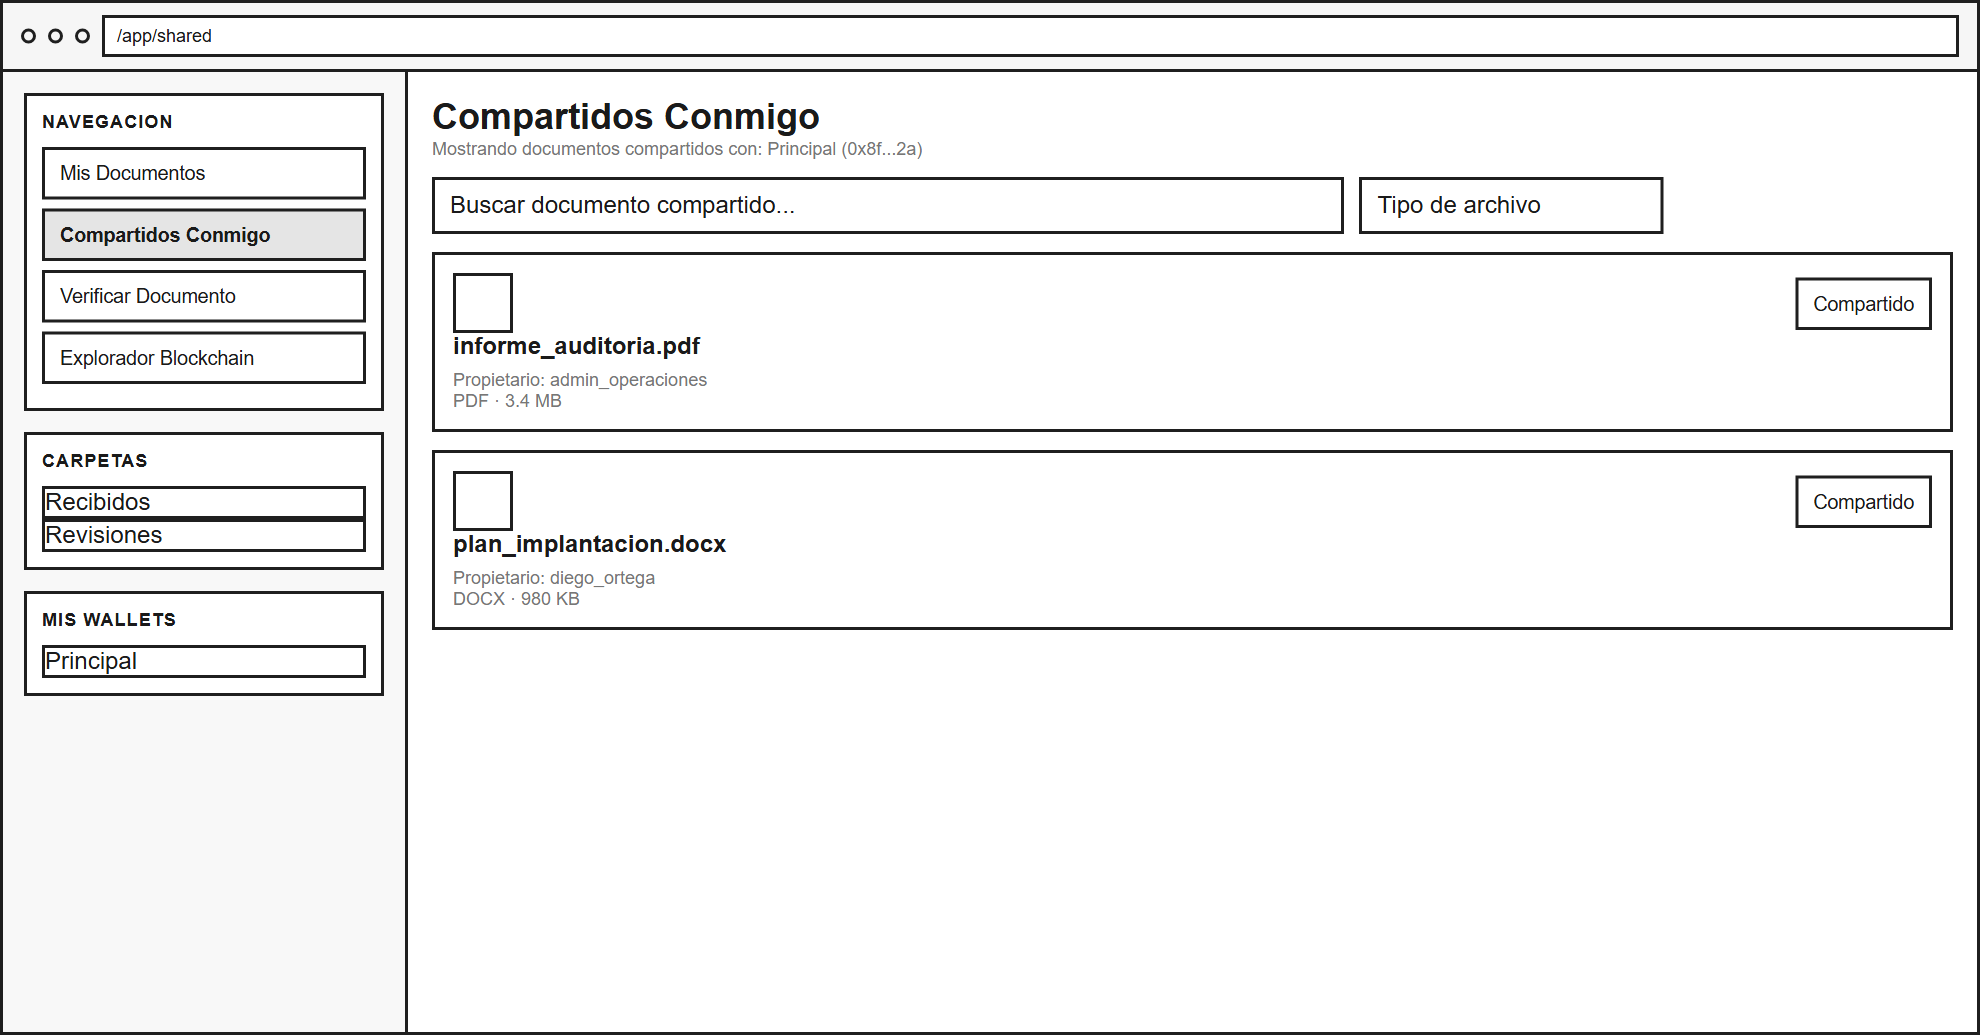
\includegraphics[width=0.87\textwidth]{bocetos-anexo2/shared-documents-wireframe.png}
    \caption{Boceto de la vista de documentos compartidos con el usuario}
    \label{fig:wf-shared}
\end{figure}

La Figura~\ref{fig:wf-admin} corresponde al panel administrativo con la gestión de usuarios y actividad.

\begin{figure}[H]
    \centering
    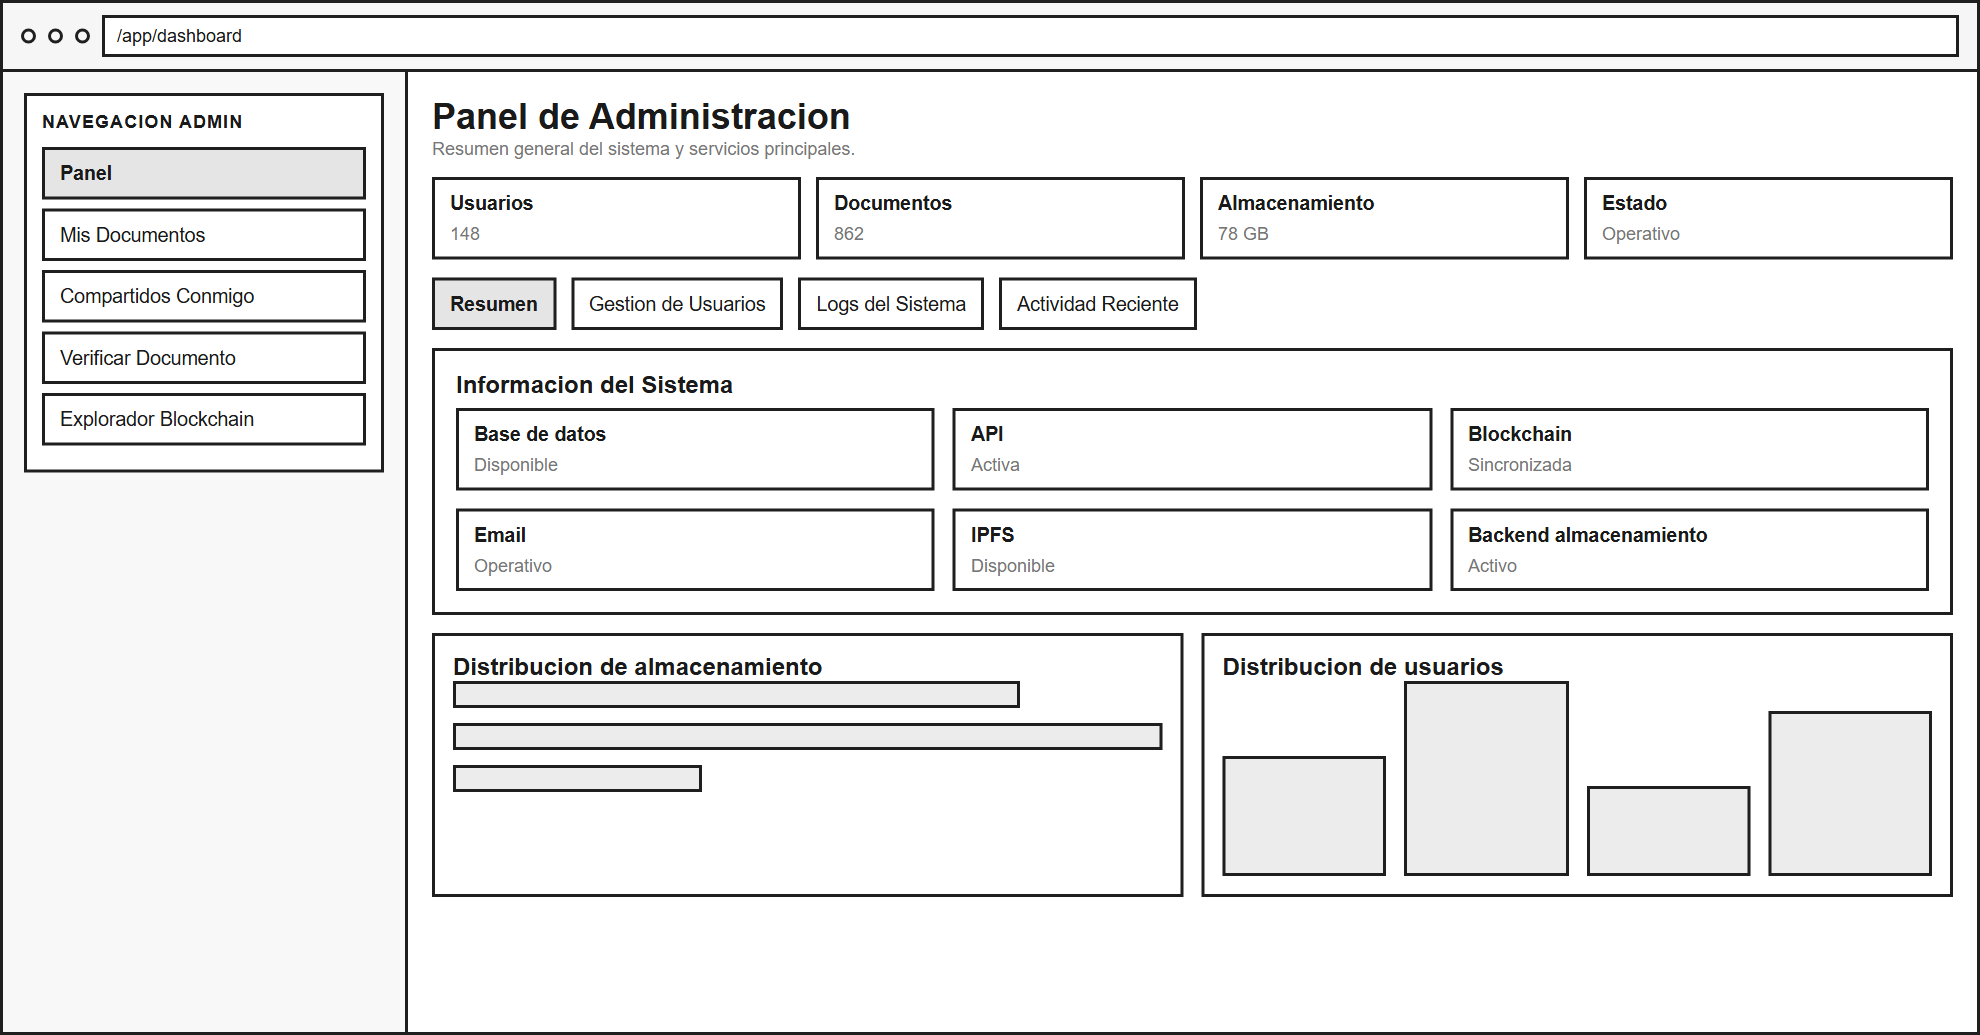
\includegraphics[width=0.87\textwidth]{bocetos-anexo2/admin-dashboard-wireframe.png}
    \caption{Boceto del panel administrativo de supervisión y control de usuarios}
    \label{fig:wf-admin}
\end{figure}

La Figura~\ref{fig:wf-blockchain} muestra la vista del explorador técnico de trazas blockchain.

\begin{figure}[H]
    \centering
    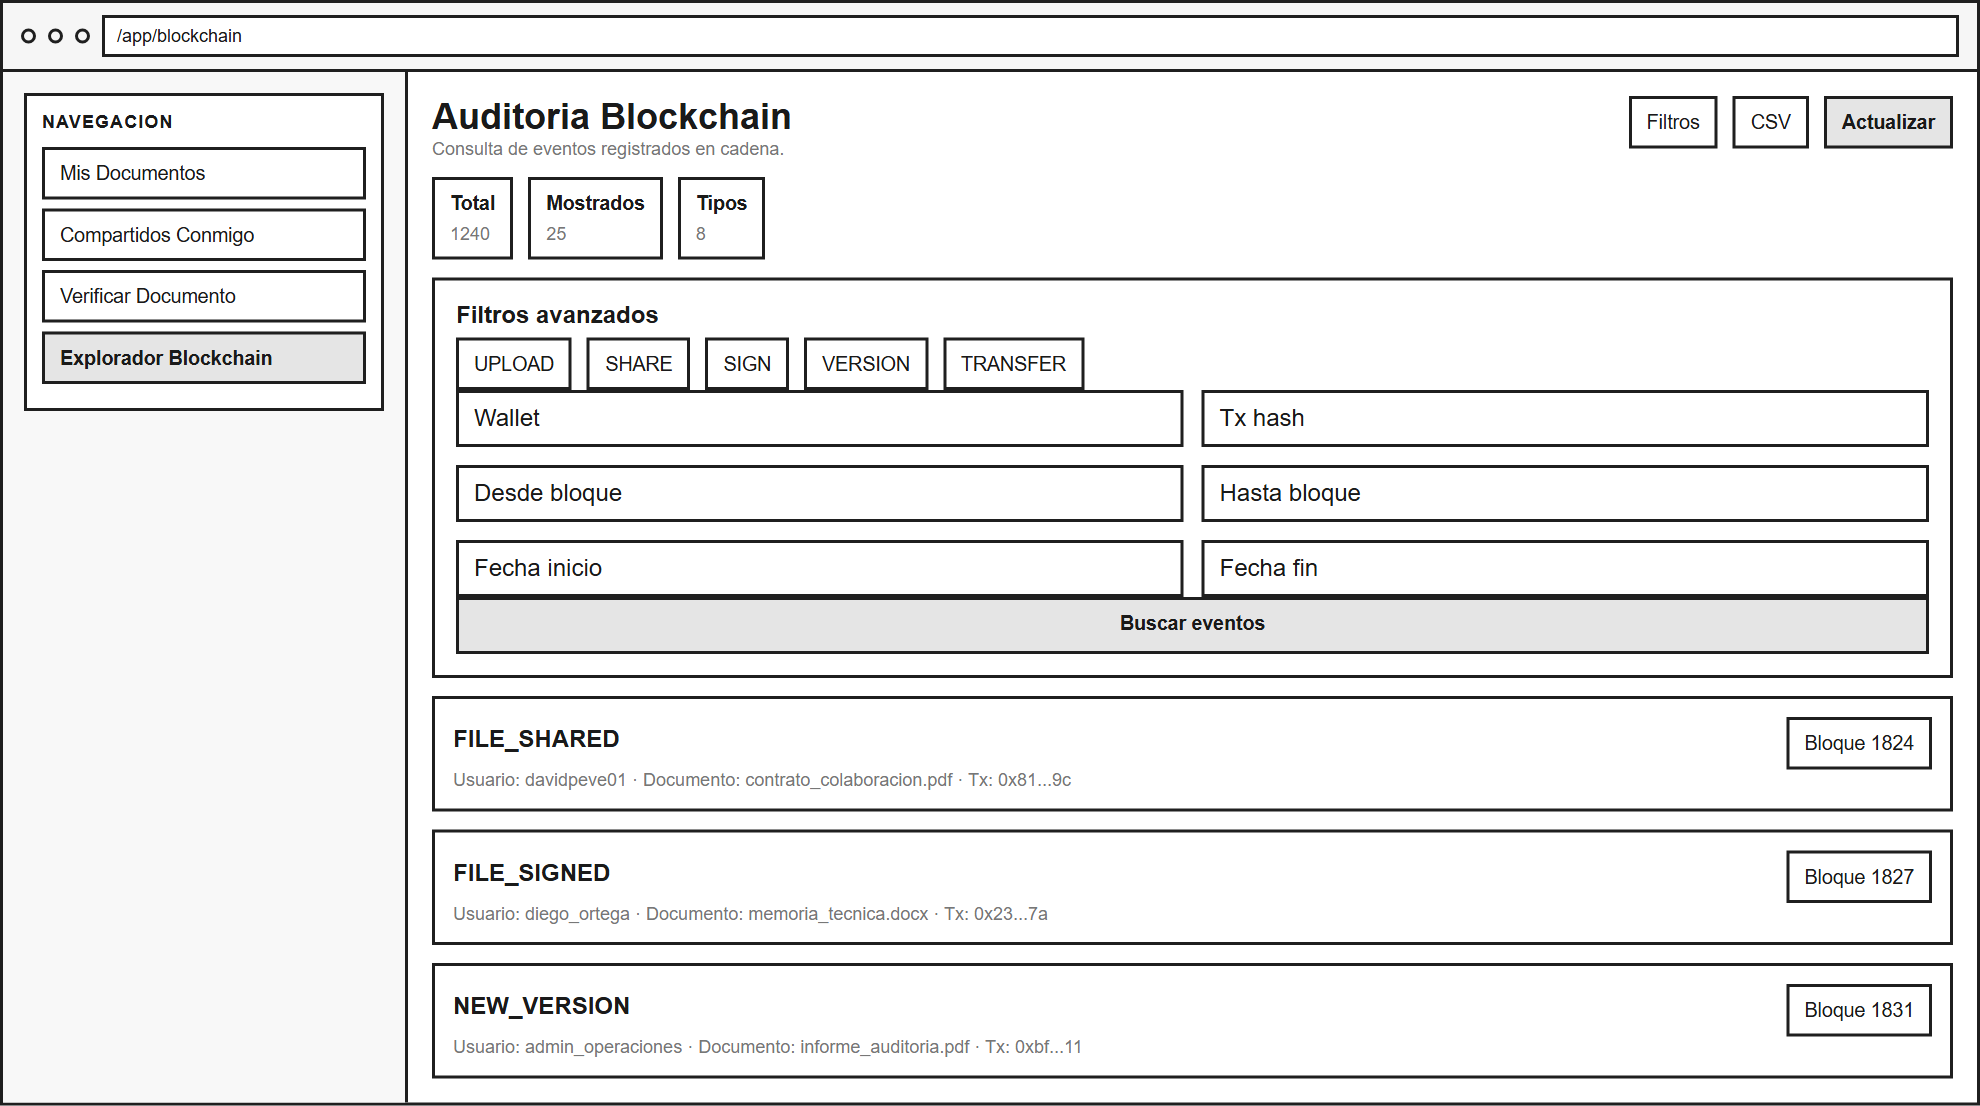
\includegraphics[width=0.87\textwidth]{bocetos-anexo2/blockchain-auditor-wireframe.png}
    \caption{Boceto del explorador técnico de evidencias blockchain integrado en la aplicación}
    \label{fig:wf-blockchain}
\end{figure}

La Figura~\ref{fig:wf-verify} corresponde a la vista pública de verificación de integridad documental.

\begin{figure}[H]
    \centering
    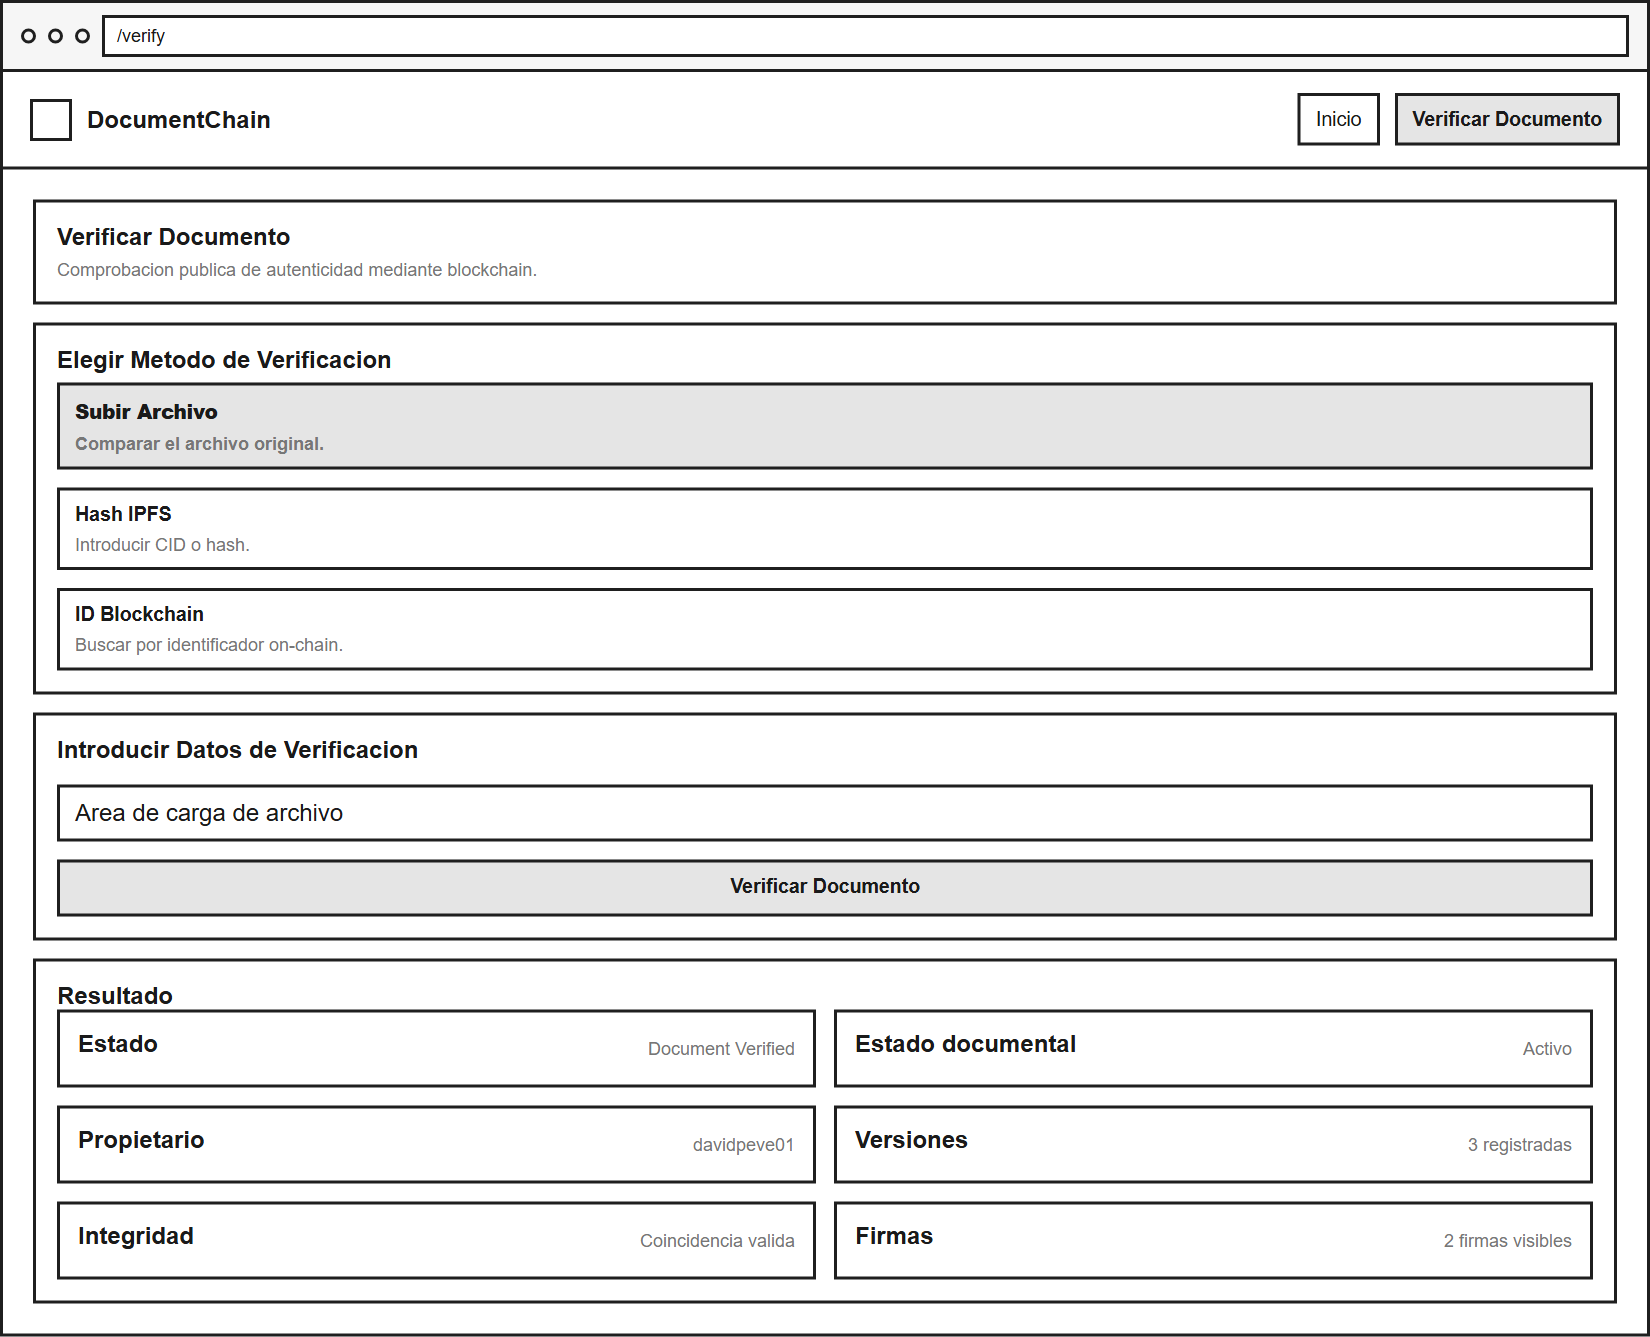
\includegraphics[width=0.82\textwidth]{bocetos-anexo2/public-verify-wireframe.png}
    \caption{Boceto de la vista pública de verificación de documento sin autenticación}
    \label{fig:wf-verify}
\end{figure}

La Figura~\ref{fig:wf-profile} muestra el boceto de la sección de perfil y wallets del usuario.

\begin{figure}[H]
    \centering
    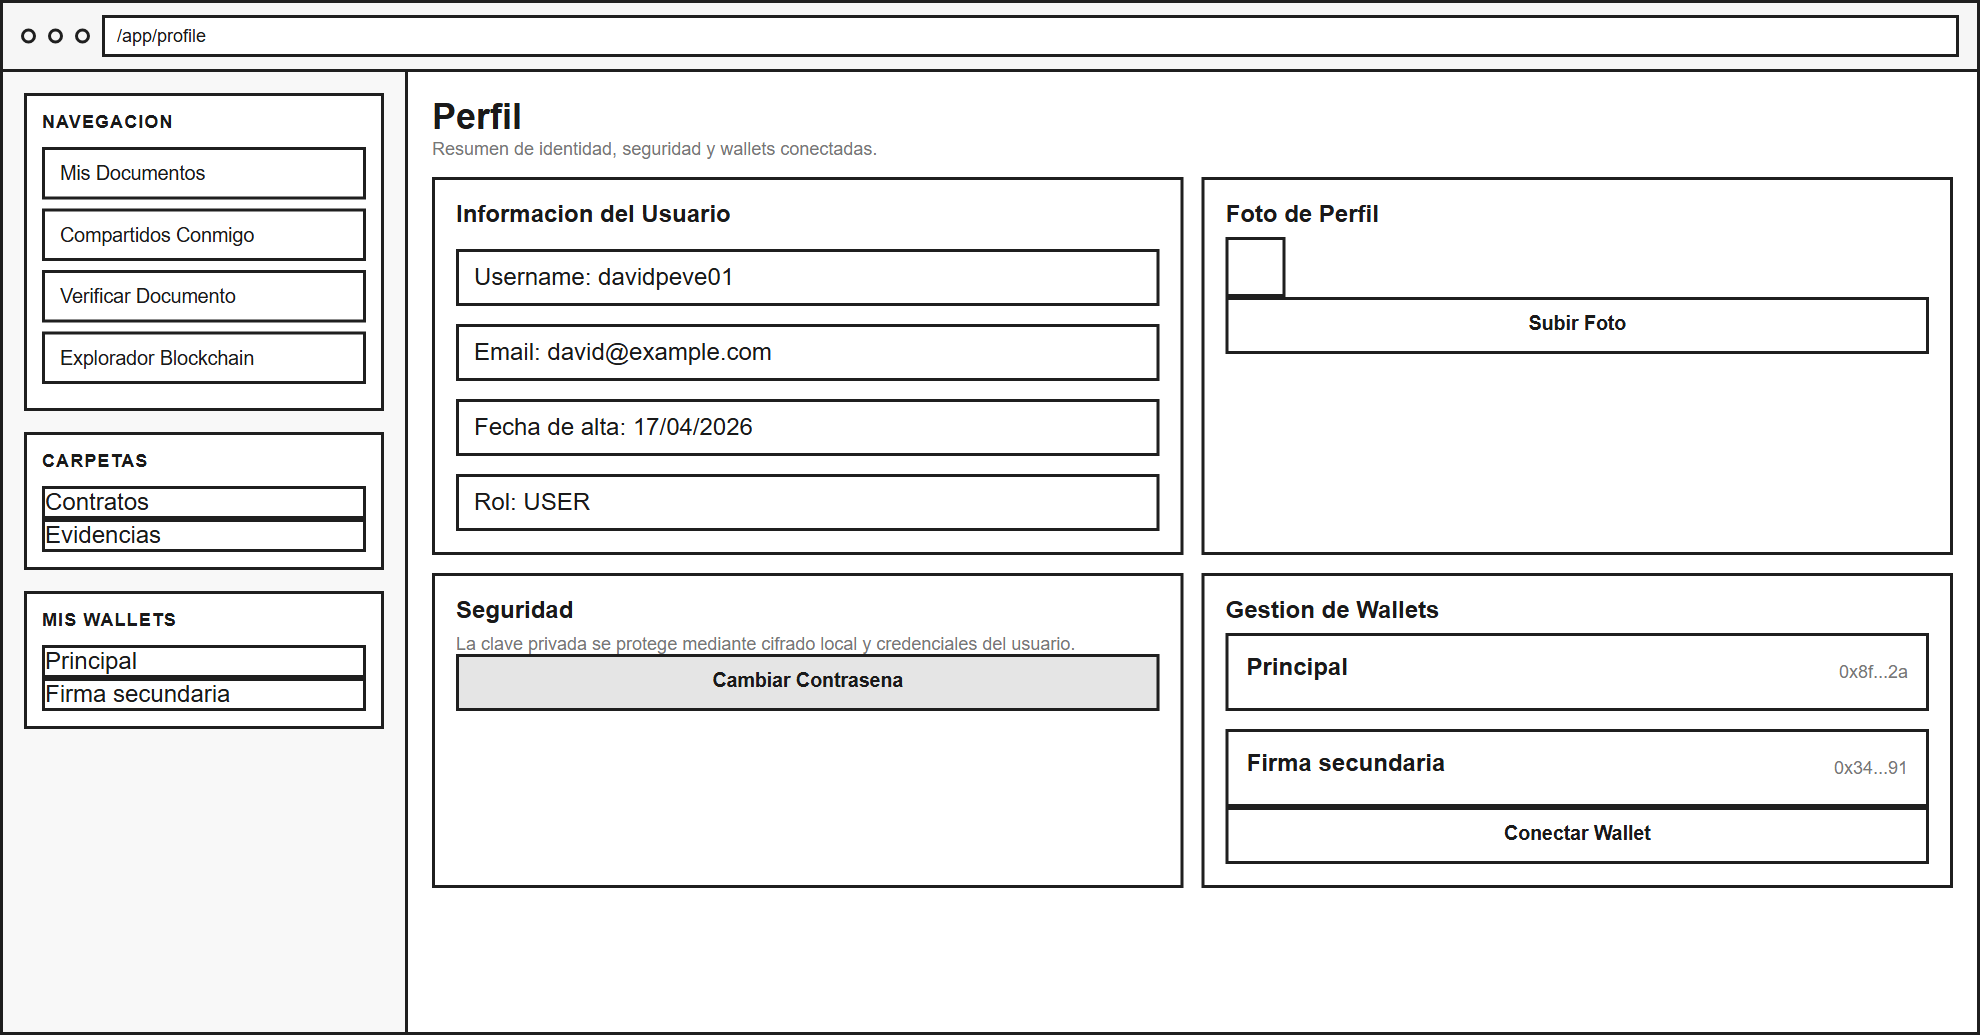
\includegraphics[width=0.82\textwidth]{bocetos-anexo2/profile-wireframe.png}
    \caption{Boceto de la sección de perfil de usuario y gestión de wallets}
    \label{fig:wf-profile}
\end{figure}

La Figura~\ref{fig:wf-settings} completa la serie con la pantalla de configuración de la cuenta.

\begin{figure}[H]
    \centering
    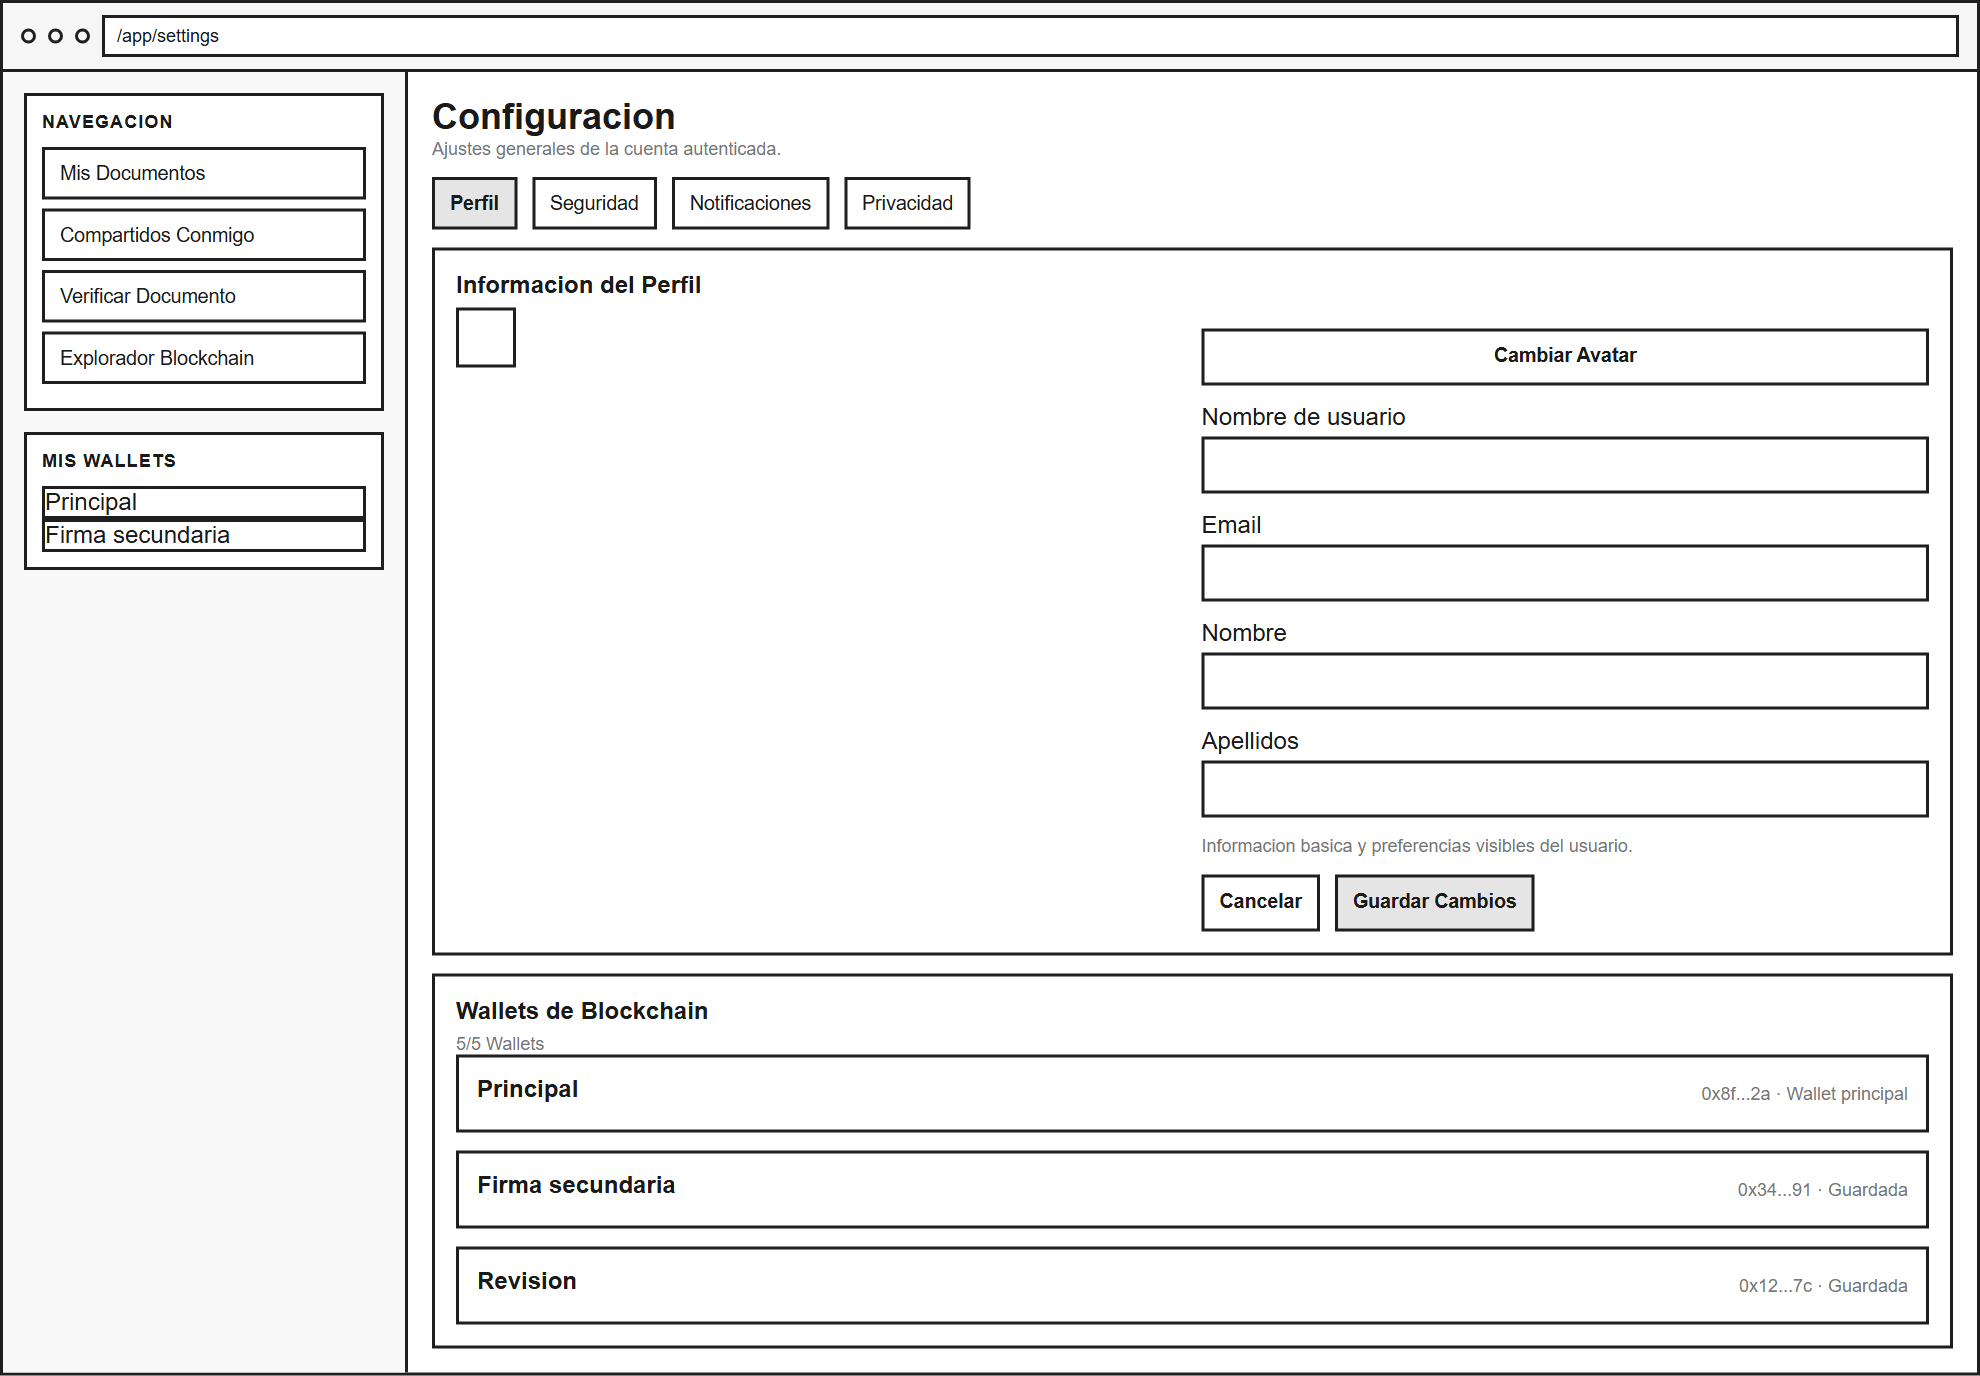
\includegraphics[width=0.82\textwidth]{bocetos-anexo2/settings-wireframe.png}
    \caption{Boceto de la pantalla de configuración y preferencias del usuario}
    \label{fig:wf-settings}
\end{figure}

La existencia de estos once bocetos tiene valor metodológico: demuestra que la interfaz evolucionó desde una representación estructural previa hacia la realización funcional final, y no fue improvista durante la construcción. El Anexo V incluye las capturas reales generadas con Playwright que permiten contrastar boceto con producto terminado.

\subsubsection{Tipografía y paleta de colores}

Las decisiones tipográficas y cromáticas de DocumentChain no se tomaron de forma arbitraria. Se adoptó Inter como fuente principal de la interfaz por su excelente legibilidad en pantallas de alta densidad y su soporte completo del conjunto de caracteres necesario para una aplicación en español con términos técnicos en inglés. Su diseño como fuente variable permite ajustar el peso tipográfico para diferenciar encabezados de contenido sin recurrir a múltiples familias, lo que contribuye a la consistencia visual del conjunto.

La paleta cromática parte de un azul oscuro (\texttt{\#1e3a5f}) como color de identidad principal, que aparece en la barra de navegación, los botones de acción primaria y los estados activos de la interfaz. Se complementa con un conjunto de colores funcionales: verde para estados activos y confirmaciones, rojo para advertencias y errores, naranja para estados intermedios y gris para contenido secundario o inactivo. El fondo principal utiliza un blanco ligeramente roto en las áreas de contenido y un gris claro en la barra lateral, lo que reduce la fatiga visual en sesiones de trabajo prolongadas.

\begin{table}[H]
    \centering
    \small
    \begin{tabular}{|p{4cm}|p{2.5cm}|p{6.5cm}|}
    \hline
    \textbf{Uso en la interfaz} & \textbf{Valor hex} & \textbf{Función visual} \\
    \hline
    Color de identidad principal & \texttt{\#1e3a5f} & Navegación, botones primarios y estados activos de selección. \\
    \hline
    Acento de acción & \texttt{\#2563eb} & Botones de confirmación, enlaces interactivos y elementos de foco. \\
    \hline
    Estado activo / correcto & \texttt{\#16a34a} & Documentos activos, confirmaciones y estados de sincronización correcta. \\
    \hline
    Advertencia / intermedio & \texttt{\#d97706} & Estados de preparación, operaciones pendientes y alertas moderadas. \\
    \hline
    Error / crítico & \texttt{\#dc2626} & Validaciones de formulario fallidas, estados de error y acciones destructivas. \\
    \hline
    Fondo principal & \texttt{\#f8fafc} & Área de contenido general de la aplicación. \\
    \hline
    Fondo secundario & \texttt{\#f1f5f9} & Barra lateral, tarjetas de contenido y secciones de apoyo. \\
    \hline
    Texto principal & \texttt{\#0f172a} & Cuerpo de texto, encabezados y etiquetas de formulario. \\
    \hline
    \end{tabular}
    \caption{Paleta de colores funcionales de la interfaz de DocumentChain}
    \label{tab:paleta-colores}
\end{table}

\subsection{Métricas}

En la memoria de referencia, las métricas ocupan un espacio relevante porque ayudan a traducir la funcionalidad a criterios observables de evaluación. En DocumentChain no existe un dispositivo biomédico que genere telemetría física comparable, pero sí un conjunto de métricas funcionales, operativas y de validación que permiten valorar el comportamiento del sistema. Este enfoque es igualmente útil desde el punto de vista académico, ya que desplaza la discusión desde la mera enumeración de módulos hacia la comprobación de qué dimensiones del sistema se pueden medir o contrastar.

\subsubsection{Métricas funcionales del dominio documental}

Las primeras métricas son las que describen la actividad documental propiamente dicha: número de documentos por usuario, volumen de versiones, cantidad de firmas registradas, documentos compartidos, recursos públicos activos y operaciones administrativas ejecutadas. Estas medidas no solo sirven para cuadros de mando futuros; también expresan qué aspectos del dominio se consideran relevantes dentro del sistema.

\begin{table}[H]
    \centering
    \small
    \begin{tabular}{|p{4cm}|p{3.5cm}|p{5.9cm}|}
    \hline
    \textbf{Métrica} & \textbf{Unidad} & \textbf{Utilidad principal} \\
    \hline
    Documentos gestionados & Número de documentos & Cuantificar el volumen principal de trabajo de cada usuario o del sistema. \\
    \hline
    Versiones por documento & Número de versiones & Medir la actividad de edición y la evolución histórica del contenido. \\
    \hline
    Firmas registradas & Número de firmas & Observar el uso efectivo de la capa de aceptación verificable. \\
    \hline
    Documentos compartidos & Número de relaciones activas & Valorar la dimensión colaborativa de la plataforma. \\
    \hline
    Recursos públicos publicados & Número de \texttt{publicId} activos & Medir la exposición deliberada de documentos o evidencias al exterior. \\
    \hline
    \end{tabular}
    \caption{Métricas funcionales asociadas al dominio documental}
    \label{tab:metricas-funcionales-documentales}
\end{table}

\subsubsection{Métricas técnicas y de integración}

La segunda familia de métricas se refiere al comportamiento técnico del sistema. Aquí interesa observar tiempos de respuesta de la API, latencia en la confirmación de operaciones blockchain, éxito de subida y recuperación desde IPFS, incidencias de sincronización y entrega de notificaciones. Aunque no todas estas medidas se presentan como un cuadro numérico cerrado en la memoria, sí constituyen criterios válidos para evaluar la calidad operativa del prototipo.

\begin{table}[H]
    \centering
    \small
    \begin{tabular}{|p{4cm}|p{3.5cm}|p{5.9cm}|}
    \hline
    \textbf{Métrica} & \textbf{Unidad} & \textbf{Interpretación} \\
    \hline
    Tiempo de respuesta API & Milisegundos/segundos & Refleja la agilidad operativa de la plataforma para consulta y gestión documental. \\
    \hline
    Tiempo de confirmación de transacción & Segundos o bloques & Mide el intervalo entre preparación y consolidación verificable de una operación crítica. \\
    \hline
    Éxito de publicación en IPFS & Tasa de operaciones correctas & Permite valorar la fiabilidad de la persistencia distribuida. \\
    \hline
    Incidencias de sincronización & Número de eventos pendientes o fallidos & Ayuda a detectar desalineaciones entre la capa operativa y la capa de evidencia. \\
    \hline
    Entrega de notificaciones & Tasa de envío/recepción & Evalúa el estado del subsistema de correo y avisos operativos. \\
    \hline
    \end{tabular}
    \caption{Métricas técnicas y de integración relevantes para el prototipo}
    \label{tab:metricas-tecnicas-memoria}
\end{table}

\subsubsection{Métricas de validación y cobertura}

Una tercera familia de métricas procede directamente del proceso de validación. En este punto cobran valor el número de pruebas automatizadas, la cobertura funcional de los escenarios extremos, la presencia de recorridos E2E y la correspondencia entre prototipos, capturas y comportamiento real. Estas métricas no describen el dominio documental, pero sí la confianza razonable que puede depositarse en la solución implementada.

La documentación actual permite afirmar que la validación se apoya en más de doscientas pruebas automatizadas repartidas entre backend y contrato inteligente, además de pruebas funcionales de sistema y evidencia visual del comportamiento de la interfaz. Para una memoria académica, esta combinación resulta especialmente útil porque refuerza la idea de que el sistema no se ha validado desde una sola perspectiva.

\section{Requisitos iniciales}

\subsection{Objetivos del sistema}

La especificación completa del sistema se desarrolla en el Anexo I, donde se catalogan los actores, los objetivos y el conjunto consolidado de casos de uso. En la memoria principal interesa recoger esa información de forma sintética para mostrar que la solución final no nace de una acumulación improvisada de funcionalidades, sino de una definición previa del alcance. Los objetivos del sistema se formulan como enunciados de alto nivel que concentran la intención del proyecto y que guían las decisiones posteriores de análisis, diseño e implementación.

\begin{table}[H]
    \centering
    \small
    \begin{tabular}{|p{4cm}|p{9cm}|}
    \hline
    \multicolumn{2}{|c|}{\textbf{Especificación del objetivo OBJ-0001}} \\
    \hline
    \textbf{Identificador} & OBJ-0001 \\
    \hline
    \textbf{Nombre} & Gestión de usuarios y seguridad de acceso \\
    \hline
    \textbf{Descripción} & El sistema debe proporcionar mecanismos seguros de registro, autenticación y administración de cuentas de usuario, incluyendo verificación de correo electrónico, recuperación de contraseña, soporte para segundo factor de autenticación y vinculación de wallets Ethereum para operaciones que requieran firma digital. \\
    \hline
    \textbf{Importancia} & Alta \\
    \hline
    \textbf{Urgencia} & Alta \\
    \hline
    \end{tabular}
    \caption{Especificación del objetivo OBJ-0001: Gestión de usuarios y seguridad de acceso}
    \label{tab:obj-0001}
\end{table}

\begin{table}[H]
    \centering
    \small
    \begin{tabular}{|p{4cm}|p{9cm}|}
    \hline
    \multicolumn{2}{|c|}{\textbf{Especificación del objetivo OBJ-0002}} \\
    \hline
    \textbf{Identificador} & OBJ-0002 \\
    \hline
    \textbf{Nombre} & Ciclo de vida documental con versionado \\
    \hline
    \textbf{Descripción} & El sistema debe soportar el ciclo de vida completo del documento digital: alta, versionado, archivado lógico, restauración de versiones anteriores y organización mediante carpetas y etiquetas (tags). Cada operación relevante debe quedar registrada en el historial de actividad asociado al documento. \\
    \hline
    \textbf{Importancia} & Alta \\
    \hline
    \textbf{Urgencia} & Alta \\
    \hline
    \end{tabular}
    \caption{Especificación del objetivo OBJ-0002: Ciclo de vida documental con versionado}
    \label{tab:obj-0002}
\end{table}

\begin{table}[H]
    \centering
    \small
    \begin{tabular}{|p{4cm}|p{9cm}|}
    \hline
    \multicolumn{2}{|c|}{\textbf{Especificación del objetivo OBJ-0003}} \\
    \hline
    \textbf{Identificador} & OBJ-0003 \\
    \hline
    \textbf{Nombre} & Trazabilidad blockchain e integración con IPFS \\
    \hline
    \textbf{Descripción} & El sistema debe registrar en una cadena de bloques los eventos documentales más significativos (creación, versionado, firma, compartición, transferencia de propiedad) mediante un contrato inteligente desplegado en una red EVM. Los archivos documentales deben almacenarse en IPFS, referenciados por su CID, para garantizar direccionamiento por contenido e independencia del backend. \\
    \hline
    \textbf{Importancia} & Alta \\
    \hline
    \textbf{Urgencia} & Alta \\
    \hline
    \end{tabular}
    \caption{Especificación del objetivo OBJ-0003: Trazabilidad blockchain e integración IPFS}
    \label{tab:obj-0003}
\end{table}

\begin{table}[H]
    \centering
    \small
    \begin{tabular}{|p{4cm}|p{9cm}|}
    \hline
    \multicolumn{2}{|c|}{\textbf{Especificación del objetivo OBJ-0004}} \\
    \hline
    \textbf{Identificador} & OBJ-0004 \\
    \hline
    \textbf{Nombre} & Verificación pública y auditoría abierta \\
    \hline
    \textbf{Descripción} & El sistema debe ofrecer un mecanismo de publicación controlada de documentos mediante el cual el propietario pueda exponer un documento o su evidencia de integridad para consulta pública sin requerir autenticación. Los verificadores externos deben poder contrastar el hash y el estado del documento directamente desde la interfaz. \\
    \hline
    \textbf{Importancia} & Media \\
    \hline
    \textbf{Urgencia} & Media \\
    \hline
    \end{tabular}
    \caption{Especificación del objetivo OBJ-0004: Verificación pública y auditoría abierta}
    \label{tab:obj-0004}
\end{table}

\begin{table}[H]
    \centering
    \small
    \begin{tabular}{|p{4cm}|p{9cm}|}
    \hline
    \multicolumn{2}{|c|}{\textbf{Especificación del objetivo OBJ-0005}} \\
    \hline
    \textbf{Identificador} & OBJ-0005 \\
    \hline
    \textbf{Nombre} & Colaboración documental con control de acceso granular \\
    \hline
    \textbf{Descripción} & El sistema debe permitir compartir documentos con otros usuarios asignando roles diferenciados (OWNER, EDITOR, VIEWER), así como revocar permisos y transferir la titularidad del documento. Las operaciones de permisos de mayor impacto deben quedar reflejadas en el registro blockchain. \\
    \hline
    \textbf{Importancia} & Alta \\
    \hline
    \textbf{Urgencia} & Media \\
    \hline
    \end{tabular}
    \caption{Especificación del objetivo OBJ-0005: Colaboración documental con control de acceso}
    \label{tab:obj-0005}
\end{table}

\begin{table}[H]
    \centering
    \small
    \begin{tabular}{|p{4cm}|p{9cm}|}
    \hline
    \multicolumn{2}{|c|}{\textbf{Especificación del objetivo OBJ-0006}} \\
    \hline
    \textbf{Identificador} & OBJ-0006 \\
    \hline
    \textbf{Nombre} & Administración de la plataforma y despliegue reproducible \\
    \hline
    \textbf{Descripción} & El sistema debe incluir un panel de administración para la supervisión de usuarios, revisión de actividad y gestión del estado global de la plataforma. Debe además poder desplegarse de forma reproducible mediante contenedores Docker, con servicios de base de datos, blockchain local, backend, frontend y correo transaccional integrados en la misma composición. \\
    \hline
    \textbf{Importancia} & Media \\
    \hline
    \textbf{Urgencia} & Media \\
    \hline
    \end{tabular}
    \caption{Especificación del objetivo OBJ-0006: Administración y despliegue reproducible}
    \label{tab:obj-0006}
\end{table}

\subsection{Síntesis funcional del sistema}

Los requisitos funcionales se agrupan en varios bloques coherentes: acceso y seguridad de cuenta, gestión documental, versionado, colaboración, firma, verificación pública y administración. La especificación completa alcanza 42 casos de uso principales agrupados en paquetes diferenciados por dominio funcional. La Figura~\ref{fig:uc-acceso-mem} muestra los casos de uso del paquete de acceso y gestión de cuenta.

\begin{figure}[H]
    \centering
    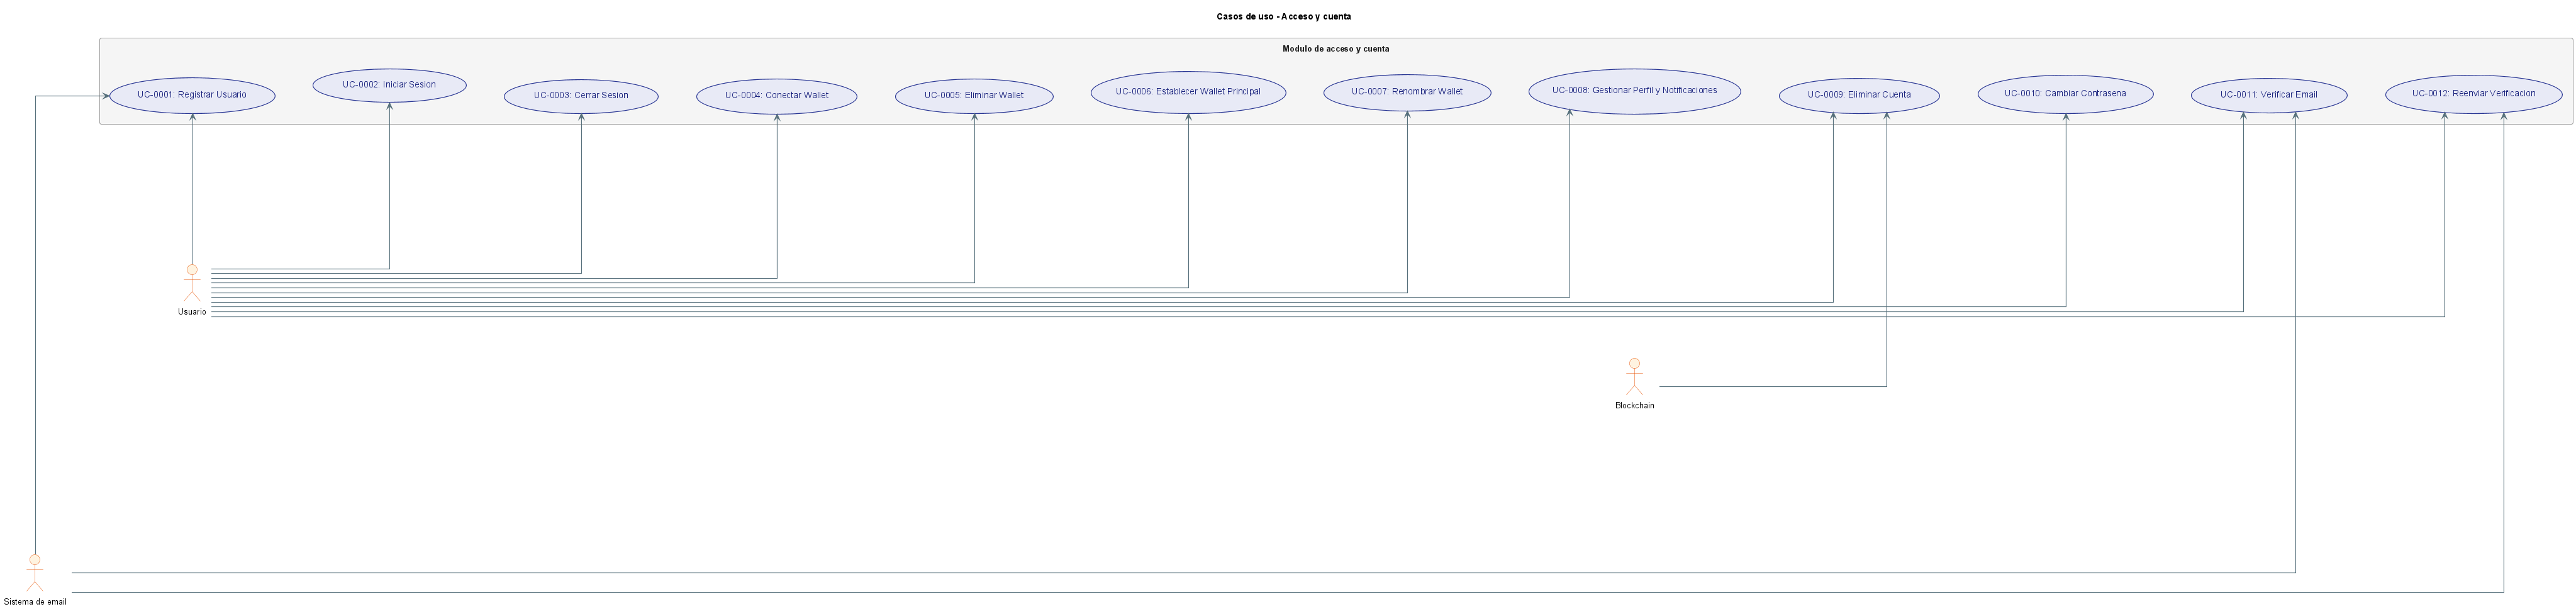
\includegraphics[width=0.88\textwidth]{diagramas/uc_acceso.png}
    \caption{Casos de uso del paquete de acceso, autenticación y gestión de cuenta}
    \label{fig:uc-acceso-mem}
\end{figure}

\begin{figure}[H]
    \centering
    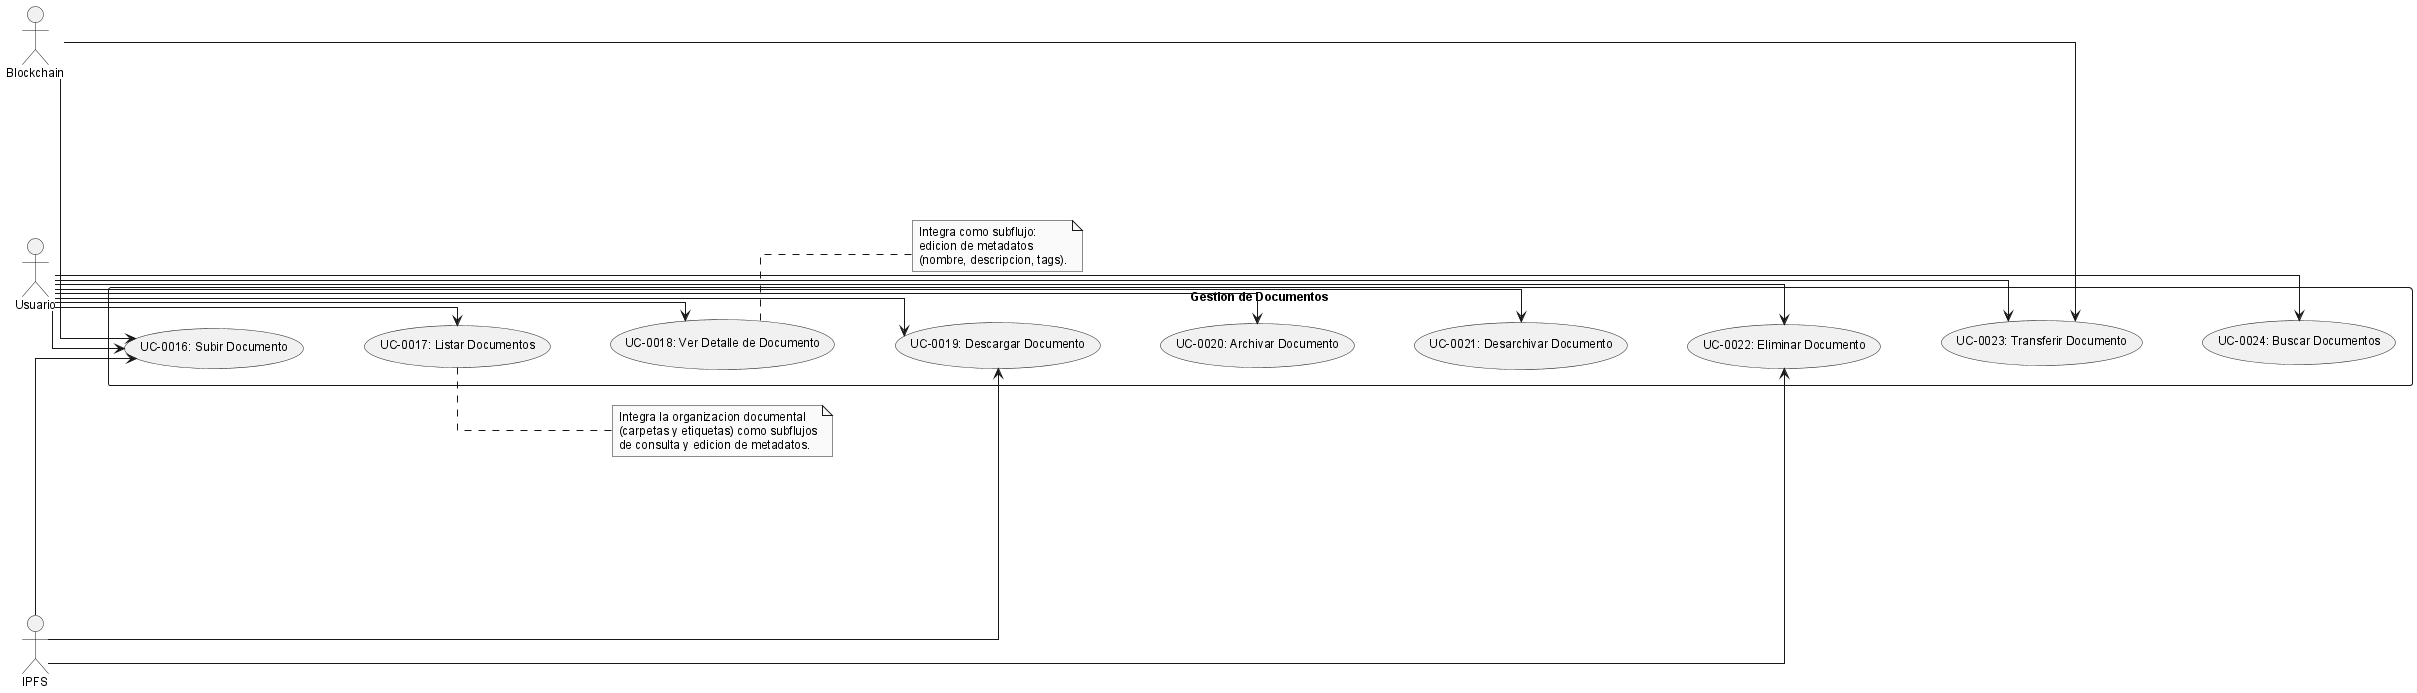
\includegraphics[width=0.88\textwidth]{diagramas/uc_documentos.png}
    \caption{Casos de uso del paquete de gestión documental y organización}
    \label{fig:uc-documentos-mem}
\end{figure}

\begin{figure}[H]
    \centering
    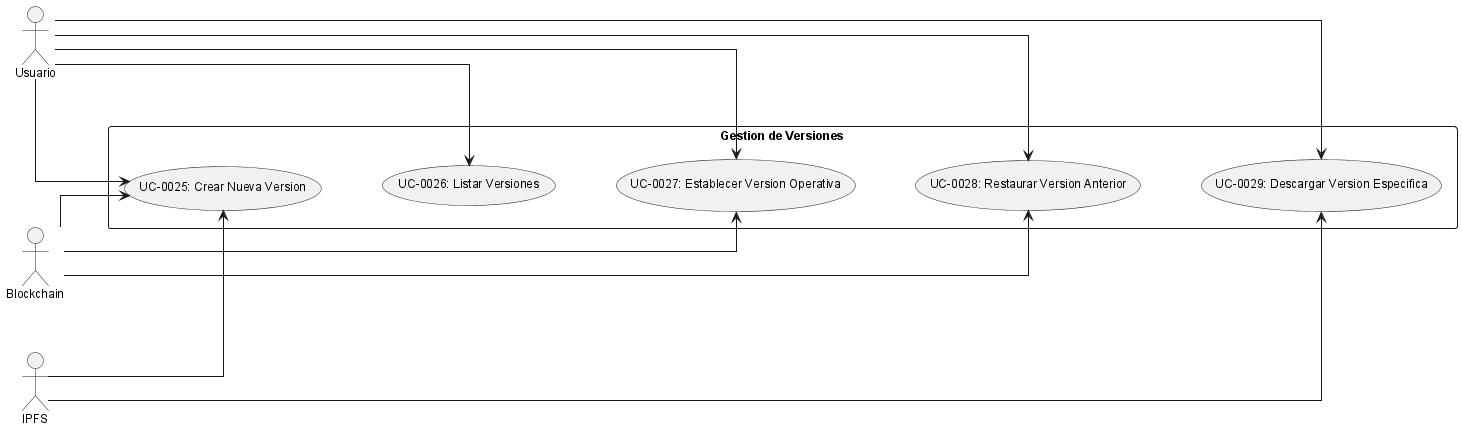
\includegraphics[width=0.88\textwidth]{diagramas/uc_versiones.png}
    \caption{Casos de uso del paquete de versionado y ciclo de vida documental}
    \label{fig:uc-versiones-mem}
\end{figure}

\begin{figure}[H]
    \centering
    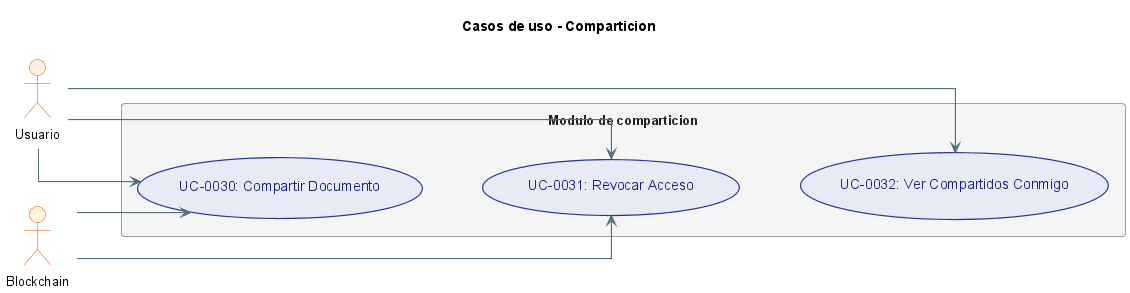
\includegraphics[width=0.88\textwidth]{diagramas/uc_comparticion.png}
    \caption{Casos de uso del paquete de compartición y control de acceso}
    \label{fig:uc-comparticion-mem}
\end{figure}

\begin{figure}[H]
    \centering
    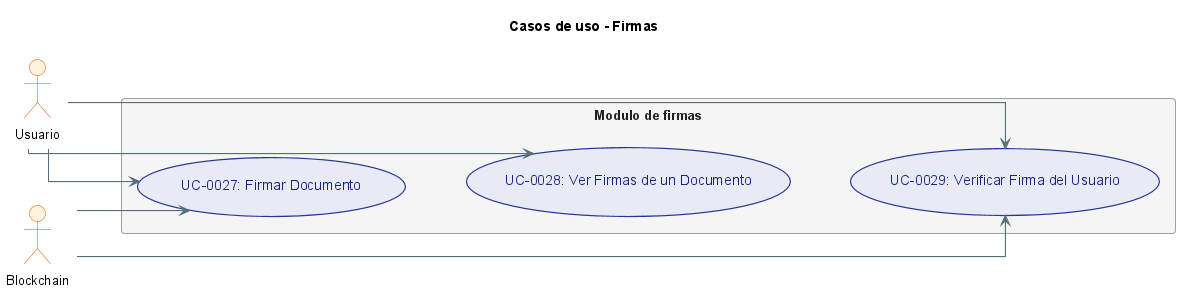
\includegraphics[width=0.88\textwidth]{diagramas/uc_firmas.png}
    \caption{Casos de uso del paquete de firma digital y trazabilidad}
    \label{fig:uc-firmas-mem}
\end{figure}

\begin{figure}[H]
    \centering
    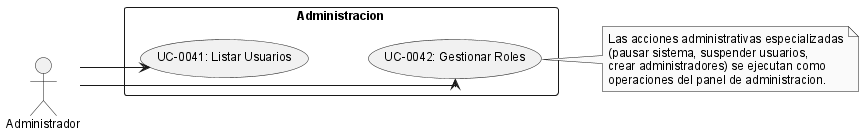
\includegraphics[width=0.88\textwidth]{diagramas/uc_administracion.png}
    \caption{Casos de uso del paquete de administración de la plataforma}
    \label{fig:uc-administracion-mem}
\end{figure}

\begin{figure}[H]
    \centering
    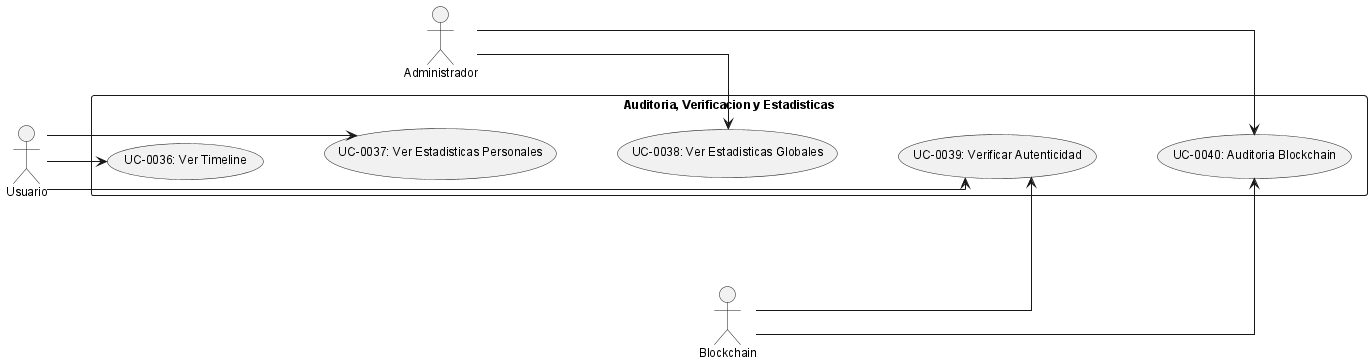
\includegraphics[width=0.88\textwidth]{diagramas/uc_auditoria.png}
    \caption{Casos de uso del paquete de auditoría y verificación pública}
    \label{fig:uc-auditoria-mem}
\end{figure}

\begin{table}[H]
    \centering
    \small
    \begin{tabular}{|p{3.8cm}|p{3.6cm}|p{5.1cm}|}
    \hline
    \textbf{Bloque funcional} & \textbf{Capacidad principal} & \textbf{Manifestación en la solución} \\
    \hline
    Acceso y cuenta & Registro, autenticación y perfil & Alta de usuario, verificación por correo, recuperación de contraseña, gestión de wallets y 2FA opcional. \\
    \hline
    Gestión documental & Alta, descarga y organización & Subida de documentos, clasificación por carpetas y etiquetas, listados y búsquedas. \\
    \hline
    Versionado y ciclo de vida & Evolución controlada del documento & Creación de versiones, restauración, archivado y reactivación de versión operativa. \\
    \hline
    Colaboración y permisos & Trabajo compartido con control granular & Roles OWNER, EDITOR y VIEWER, compartición, revocación y transferencia de propiedad. \\
    \hline
    Firma y evidencia & Vinculación de acciones a la wallet del usuario & Firma digital, registro on-chain y conservación de la evidencia asociada. \\
    \hline
    Publicación y verificación & Exposición selectiva de contenido o prueba & Enlaces públicos, auditoría pública y consulta verificable de documentos publicados. \\
    \hline
    Administración & Supervisión global del sistema & Panel de control, gestión de usuarios, consulta de actividad y revisión del estado global. \\
    \hline
    \end{tabular}
    \caption{Síntesis de requisitos funcionales agrupados por bloques}
    \label{tab:requisitos-funcionales-sintesis}
\end{table}

\subsection{Actores técnicos y externos}

Además de los perfiles humanos, el proyecto depende de varios actores no humanos que condicionan su diseño. El contrato inteligente actúa como fuente de verdad para la evidencia blockchain; el nodo IPFS autoalojado conserva el binario direccionado por contenido; y el subsistema de correo articula la mensajería transaccional necesaria para registro, recuperación y notificaciones. Esta identificación temprana de actores técnicos fue importante porque obligó a modelar el sistema como una integración entre componentes heterogéneos y no como una simple aplicación web autocontenida.

\subsection{Criterios no funcionales principales}

La solución no solo debía ofrecer funciones, sino cumplir condiciones de calidad suficientes para ser defendible técnica y académicamente. En la especificación se definieron requisitos no funcionales relativos a seguridad, rendimiento, usabilidad, disponibilidad y mantenibilidad. Su interés radica en que anticipan decisiones que luego aparecen en la implementación, como el uso de cifrado autenticado, límites operativos para archivos, validación estricta de entrada, tipado fuerte o documentación de despliegue.

\begin{table}[H]
    \centering
    \small
    \begin{tabular}{|p{2.4cm}|p{3.5cm}|p{6.6cm}|}
    \hline
    \textbf{Código} & \textbf{Criterio} & \textbf{Concreción principal en el proyecto} \\
    \hline
    NFR-0001 & Seguridad y privacidad & Cifrado AES-256-GCM para documentos privados, Argon2id para credenciales, validación estricta y separación entre autenticación y firma. \\
    \hline
    NFR-0002 & Rendimiento y escalabilidad & Límites de tamaño razonables, consultas indexadas, paginación y estrategia preparada para concurrencia moderada. \\
    \hline
    NFR-0003 & Usabilidad & Interfaz responsive, feedback visible en operaciones asíncronas, formularios validados y recorridos coherentes. \\
    \hline
    NFR-0004 & Disponibilidad y tolerancia a fallos & Estados intermedios, \textit{health checks}, servicios desacoplados y patrón \textit{prepare/confirm}. \\
    \hline
    NFR-0005 & Mantenibilidad y documentación & TypeScript estricto, separación por capas, guías de arranque, anexos técnicos y validación automatizada. \\
    \hline
    \end{tabular}
    \caption{Resumen de criterios no funcionales relevantes para la memoria}
    \label{tab:requisitos-no-funcionales-sintesis}
\end{table}

\subsection{Requisitos funcionales representativos}

La especificación completa contempla 42 casos de uso principales, pero la memoria puede sintetizar ese catálogo en torno a un conjunto más reducido de capacidades nucleares. Lo relevante no es enumerar exhaustivamente todos los casos de uso en este punto, sino mostrar que la implementación desarrollada responde a un modelo funcional consistente desde el acceso a la cuenta hasta la verificación pública del documento.

\begin{table}[H]
    \centering
    \small
    \begin{tabular}{|p{2.2cm}|p{3.6cm}|p{7.3cm}|}
    \hline
    \textbf{Código} & \textbf{Requisito funcional} & \textbf{Concreción resumida} \\
    \hline
    RF-01 & Gestión de acceso e identidad & Registro, inicio de sesión, verificación por correo, recuperación de contraseña, configuración de perfil y vinculación de wallets. \\
    \hline
    RF-02 & Gestión documental & Alta de documentos, organización por carpetas y etiquetas, consulta, descarga y archivado lógico. \\
    \hline
    RF-03 & Versionado y ciclo de vida & Creación de nuevas versiones, restauración de versiones anteriores y selección de versión operativa. \\
    \hline
    RF-04 & Compartición y permisos & Concesión y revocación de acceso con roles OWNER, EDITOR y VIEWER, además de transferencia de titularidad. \\
    \hline
    RF-05 & Firma y trazabilidad & Registro de firmas con wallet, consulta de eventos y preservación de evidencia asociada al documento. \\
    \hline
    RF-06 & Verificación pública y administración & Publicación deliberada mediante \texttt{publicId}, auditoría abierta y panel administrativo de supervisión. \\
    \hline
    \end{tabular}
    \caption{Resumen de requisitos funcionales nucleares en la memoria principal}
    \label{tab:rf-nucleares-memoria}
\end{table}

\subsection{Requisitos no funcionales representativos}

Los requisitos no funcionales determinan en gran medida la credibilidad de la solución. En un sistema como DocumentChain no basta con que las operaciones existan; también es necesario que se comporten con un nivel razonable de seguridad, claridad de uso, trazabilidad y mantenibilidad. Este plano es especialmente importante porque muchas de las decisiones arquitectónicas del proyecto solo se entienden bien cuando se observan a la luz de restricciones no funcionales concretas.

Así, el uso de cifrado autenticado no responde solo a una preferencia técnica, sino a la necesidad de proteger documentos privados fuera del backend. La contenerización no responde solo a comodidad de arranque, sino a exigencias de reproducibilidad. Y el patrón \textit{prepare/confirm} no responde solo a elegancia de diseño, sino a la necesidad de mantener consistencia entre estado operativo y evidencia blockchain. La Tabla~\ref{tab:nfr-resumen-memoria} resume esa relación.

\begin{table}[H]
    \centering
    \small
    \begin{tabular}{|p{2.3cm}|p{3.6cm}|p{7.2cm}|}
    \hline
    \textbf{Código} & \textbf{Requisito no funcional} & \textbf{Respuesta de diseño asociada} \\
    \hline
    NFR-01 & Seguridad y privacidad & AES-256-GCM, Argon2id, separación entre autenticación y firma, publicación pública solo expresa y validación de permisos. \\
    \hline
    NFR-02 & Rendimiento y consulta operativa & PostgreSQL como persistencia relacional, paginación, proyecciones de consulta y separación de la evidencia on-chain. \\
    \hline
    NFR-03 & Usabilidad & Interfaz guiada, vistas diferenciadas, feedback en operaciones asíncronas y reducción de firmas al mínimo necesario. \\
    \hline
    NFR-04 & Disponibilidad y tolerancia a fallos & Docker Compose, servicios desacoplados, estados intermedios y reconciliación posterior de transacciones. \\
    \hline
    NFR-05 & Mantenibilidad & TypeScript, Prisma, separación por capas, anexos especializados y batería de pruebas automatizadas. \\
    \hline
    \end{tabular}
    \caption{Resumen de requisitos no funcionales y su reflejo en la solución}
    \label{tab:nfr-resumen-memoria}
\end{table}

\subsection{De la especificación a la validación}

Una cuestión relevante en un trabajo de estas características es que la especificación no quede desconectada del producto final. En DocumentChain existe una relación clara entre los requisitos iniciales y las evidencias presentadas más adelante en la memoria. Los objetivos funcionales reaparecen en la arquitectura y en las capturas de la interfaz; los criterios no funcionales se reflejan en las decisiones de seguridad, despliegue y pruebas; y los actores identificados en la fase inicial vuelven a aparecer en los diagramas, en la organización de permisos y en los manuales de uso. Esta continuidad permite defender que la solución implementada responde realmente al problema que se definió al inicio.

\section{Hipótesis, restricciones y alcance}

\subsection{Hipótesis de partida}

El sistema se ha concebido bajo varias hipótesis de partida que condicionan su comportamiento y también la interpretación de sus resultados. Se presupone la existencia de usuarios que operan desde navegadores modernos, con acceso a una wallet compatible cuando una operación requiere firma blockchain. Se presupone igualmente un entorno de ejecución donde el backend pueda acceder a PostgreSQL, al nodo Kubo autoalojado configurado y a una red EVM de desarrollo o de pruebas. En el plano funcional se asume que la mayor parte de la gestión documental seguirá siendo privada y que la publicación pública constituye una decisión expresa y minoritaria, no el comportamiento por defecto del sistema.

También se parte de la hipótesis de que la blockchain debe actuar como capa de evidencia y no como sustituto universal de la base de datos. Esta premisa organiza muchas decisiones posteriores: limita la información publicada on-chain, concentra en PostgreSQL el estado operativo y desplaza a IPFS el binario documental. Si esa hipótesis no se aceptara, el proyecto sería otro y exigiría un diseño radicalmente distinto.

\subsection{Restricciones del proyecto}

La principal restricción del trabajo es su naturaleza académica y su desarrollo por una única persona en un periodo temporal acotado. Esa limitación afecta tanto al alcance como a la profundidad con la que pueden cerrarse ciertos aspectos de infraestructura real. No se ha perseguido una explotación productiva completa con red pública permanente, dominio corporativo, claves gestionadas por HSM, sistema de observabilidad integral o integración con servicios empresariales de firma electrónica. En su lugar se ha priorizado una solución defendible, funcional y reproducible en un entorno controlado.

Otra restricción relevante procede del propio ecosistema técnico. La entrega fiable de correo a Internet no depende exclusivamente del código de la aplicación, sino también de reputación de dominio, DNS y política del proveedor de salida. La experiencia de firma depende asimismo de la wallet del usuario y de la disponibilidad de la red configurada. Y la persistencia distribuida requiere aceptar que el direccionamiento por contenido de IPFS no se comporta como un sistema de ficheros mutable tradicional.

\begin{table}[H]
    \centering
    \small
    \begin{tabular}{|p{3.5cm}|p{3.2cm}|p{6.4cm}|}
    \hline
    \textbf{Restricción} & \textbf{Origen} & \textbf{Efecto sobre el proyecto} \\
    \hline
    Desarrollo individual & Académico y organizativo & Obliga a priorizar integración funcional y a acotar automatizaciones avanzadas de operación. \\
    \hline
    Entorno blockchain no productivo & Tecnológico y temporal & La validación se centra en Hardhat y redes de prueba, no en explotación pública continuada. \\
    \hline
    Dependencia de infraestructura SMTP externa & Operativo & La entrega real de correo exige relay autenticado o dominio correctamente configurado. \\
    \hline
    Gestión externa de wallet por el usuario & Funcional y de seguridad & La aplicación no custodia la clave privada y debe coordinar operaciones firmadas desde cliente. \\
    \hline
    Persistencia distribuida por CID & Arquitectónico & El borrado y la sustitución documental se modelan como nuevos estados y nuevas referencias, no como reescritura directa del binario. \\
    \hline
    \end{tabular}
    \caption{Restricciones principales asumidas en el desarrollo del proyecto}
    \label{tab:restricciones-proyecto}
\end{table}

\subsection{Alcance del trabajo}

El alcance efectivo del proyecto incluye los flujos centrales necesarios para sostener una plataforma documental verificable: gestión de cuentas, autenticación reforzable, asociación de wallets, alta de documentos, versionado, firma, compartición, transferencia, archivado, publicación pública, auditoría, administración, notificaciones y despliegue reproducible. También incluye la documentación técnica y académica necesaria para justificar el análisis, el diseño, la planificación, la seguridad y la validación del sistema.

Quedan fuera del alcance otras líneas que podrían ser razonables en una evolución posterior, como la integración con prestadores cualificados de firma, la custodia empresarial de claves, la ejecución sobre una infraestructura blockchain pública de explotación continuada, la alta disponibilidad multi-nodo de todos los servicios o la observabilidad propia de un sistema en producción institucional. Estas ausencias no invalidan el resultado alcanzado; delimitan, más bien, el tipo de entrega que corresponde a un TFG.

\subsection{Impacto esperado}

El impacto esperado del trabajo se sitúa en dos planos. En el plano técnico, se demuestra que es posible integrar base de datos relacional, almacenamiento distribuido, evidencias blockchain y protección criptográfica en una plataforma documental coherente. En el plano académico, el proyecto sirve como caso de estudio sobre cómo repartir responsabilidades entre componentes heterogéneos sin caer ni en el centralismo completo ni en el sobredimensionamiento on-chain.

Ese impacto no debe medirse solo por el número de funcionalidades implementadas. También se aprecia en la capacidad del sistema para servir como base argumental ante un tribunal: permite discutir arquitectura, seguridad, trazabilidad, pruebas, despliegue, privacidad y viabilidad con apoyo en artefactos reales, no en una demostración parcial o puramente conceptual.

\section{Estudio de alternativas y viabilidad}

\subsection{Criterio general de selección tecnológica}

Las decisiones tecnológicas del proyecto no se han tomado como una suma de preferencias aisladas. Se han evaluado en relación con cinco criterios principales: adecuación al problema documental, mantenibilidad, facilidad de integración con el resto de componentes, viabilidad académica y capacidad de despliegue reproducible. El resultado de esa evaluación conduce a un stack claramente orientado a integración entre servicios, no a especialización extrema en una única capa.

\subsection{Alternativas para frontend y experiencia de usuario}

Para la capa de presentación se podrían haber adoptado distintas rutas. Frameworks más cerrados ofrecen estructura fuerte desde el inicio, mientras que soluciones más flexibles exigen ensamblar más piezas, pero permiten adaptar mejor el proyecto a sus necesidades reales. En este contexto se optó por React con Vite y TypeScript por tres motivos principales: rapidez de iteración, ecosistema amplio y buena compatibilidad con librerías de formularios, tipado, enrutado, consumo de API e integración con wallet.

El proyecto podría haberse desarrollado también sobre Angular o Vue. Angular aporta una estructura empresarial muy definida, aunque introduce más peso conceptual y de configuración para el alcance del TFG. Vue presenta una curva de adopción amable y una composición limpia, pero el entorno ya estaba claramente orientado a React y a un conjunto de librerías que encajaban bien con el flujo documental previsto. La Tabla~\ref{tab:alternativas-frontend} resume esa valoración.

\begin{table}[H]
    \centering
    \small
    \begin{tabular}{|p{2.7cm}|p{3.4cm}|p{6.8cm}|}
    \hline
    \textbf{Alternativa} & \textbf{Ventaja principal} & \textbf{Motivo de descarte o adopción} \\
    \hline
    Angular & Estructura fuerte y ecosistema empresarial & Más pesado para un TFG con necesidad de iteración rápida y alcance modular. \\
    \hline
    Vue & Curva de aprendizaje amable y enfoque por componentes & Viable, pero con menor alineación respecto al stack finalmente consolidado en el proyecto. \\
    \hline
    React + Vite + TypeScript & Flexibilidad, ecosistema maduro y velocidad de desarrollo & Opción adoptada por equilibrio entre tipado, librerías disponibles e integración con wallet y rutas. \\
    \hline
    \end{tabular}
    \caption{Análisis resumido de alternativas para el frontend}
    \label{tab:alternativas-frontend}
\end{table}

\subsection{Alternativas para backend y API}

En la capa de servicios la comparación más razonable se establece entre marcos muy estructurados como Spring Boot, soluciones ligeras en Python y un backend sobre Node.js. Spring Boot ofrece robustez y una organización empresarial muy sólida, pero su adopción habría elevado el coste de desarrollo y la carga de configuración para el contexto del trabajo. Python facilita prototipado y dispone de un ecosistema amplio, aunque la coexistencia con el frontend habría introducido un cambio de lenguaje y de herramientas sin una ventaja decisiva para el caso concreto.

Node.js y Express se adoptaron porque encajan con una API intensiva en integración, con flujo de eventos, uso frecuente de operaciones asíncronas e intercambio constante entre almacenamiento, blockchain y notificaciones. A ello se suma el beneficio práctico de mantener TypeScript tanto en backend como en frontend, lo que simplifica modelos de datos, tipado mental y velocidad de iteración.

\begin{table}[H]
    \centering
    \small
    \begin{tabular}{|p{2.9cm}|p{3.1cm}|p{6.9cm}|}
    \hline
    \textbf{Alternativa} & \textbf{Fortaleza} & \textbf{Valoración en el contexto del proyecto} \\
    \hline
    Java + Spring Boot & Robustez y madurez empresarial & Muy sólido, pero sobredimensionado para el alcance académico y menos ágil en iteración. \\
    \hline
    Python + framework web & Rapidez de prototipado & Interesante para servicios concretos, aunque menos homogéneo con el resto del stack. \\
    \hline
    Node.js + Express + Prisma & Integración asíncrona, ecosistema amplio y homogeneidad con TypeScript & Opción adoptada por equilibrio entre sencillez, mantenibilidad e integración con el resto de capas. \\
    \hline
    \end{tabular}
    \caption{Alternativas consideradas para la capa backend}
    \label{tab:alternativas-backend}
\end{table}

\subsection{Alternativas para la persistencia operativa}

La base de datos debía soportar relaciones claras entre usuarios, wallets, documentos, versiones, firmas, eventos y notificaciones. Esa necesidad favorecía claramente una solución relacional. PostgreSQL se eligió frente a alternativas documentales porque el modelo del proyecto presenta integridad referencial explícita, relaciones múltiples y consultas operativas que se benefician del esquema relacional. Frente a otras opciones relacionales, PostgreSQL ofrecía madurez, compatibilidad con Prisma y una buena adecuación al despliegue local o dockerizado.

\subsection{Alternativas para almacenamiento documental}

El almacenamiento del binario podía haberse resuelto con sistema de ficheros local, almacenamiento objeto tradicional o IPFS. La primera opción simplificaba la infraestructura, pero reducía el valor del direccionamiento por contenido y la posibilidad de asociar el archivo a una referencia verificable. El almacenamiento objeto convencional habría sido perfectamente válido, aunque restaba interés al componente de persistencia distribuida y a la relación directa entre CID y versión documental. Por ello se adoptó IPFS mediante un nodo Kubo autoalojado, que mantiene el control del almacenamiento, la continuidad operativa y la coherencia con el despliegue completo del sistema en infraestructura propia.

\begin{table}[H]
    \centering
    \small
    \begin{tabular}{|p{3cm}|p{3.2cm}|p{6.7cm}|}
    \hline
    \textbf{Alternativa} & \textbf{Ventaja principal} & \textbf{Motivo de adopción o descarte} \\
    \hline
    Sistema de ficheros local & Simplicidad inicial & Poco alineado con el objetivo de trazabilidad y desacoplamiento del binario. \\
    \hline
    Almacenamiento objeto tradicional & Madurez y buen rendimiento & Viable, pero sin el valor conceptual del direccionamiento por contenido. \\
    \hline
    IPFS con nodo autoalojado & Control operativo y soberanía de datos & Opción finalmente adoptada por su encaje con el despliegue en infraestructura propia, la persistencia bajo control directo y la ausencia de dependencia funcional de terceros. \\
    \hline
    \end{tabular}
    \caption{Alternativas para la capa de almacenamiento documental}
    \label{tab:alternativas-almacenamiento}
\end{table}

\subsection{Alternativas para trazabilidad y evidencia}

El problema central del proyecto podía resolverse sin blockchain, apoyándose únicamente en auditoría interna firmada por el backend. Esa alternativa simplificaba el desarrollo, pero eliminaba precisamente la capa de verificabilidad externa que da sentido al trabajo. También era posible diseñar varios contratos independientes para permisos, firmas y versionado. Sin embargo, una solución tan fragmentada habría incrementado el número de transacciones, la complejidad de sincronización y el esfuerzo de integración con el frontend. La opción finalmente adoptada, un contrato consolidado sobre Hardhat, equilibra interés técnico, simplicidad de uso y viabilidad de demostración.

\subsection{Alternativas para despliegue}

En cuanto a despliegue, podían seguirse al menos tres caminos: ejecución puramente local con procesos manuales, desarrollo híbrido mezclando contenedores y procesos en caliente, o contenerización completa. La primera opción era la más ligera en infraestructura, pero la menos reproducible. La segunda es útil durante desarrollo, y de hecho el proyecto la contempla. La tercera se ha tomado como referencia principal para entrega y defensa porque ofrece mayor estabilidad narrativa y técnica: todos los servicios relevantes quedan definidos y coordinados en la misma orquestación.

\subsection{Viabilidad técnica, operativa y económica}

Desde el punto de vista técnico, el proyecto es viable porque se apoya en componentes maduros, bien documentados y compatibles entre sí. Desde el punto de vista operativo, resulta viable porque puede ejecutarse localmente con Docker Compose sin requerir infraestructura corporativa. Y desde el punto de vista económico, también es razonable para un TFG, ya que la mayor parte del stack utilizado es de código abierto y los costes adicionales quedan desplazados a la infraestructura de despliegue y a servicios opcionales, como un proveedor SMTP.

\begin{table}[H]
    \centering
    \small
    \begin{tabular}{|p{3.5cm}|p{2.2cm}|p{6.7cm}|}
    \hline
    \textbf{Dimensión de viabilidad} & \textbf{Valoración} & \textbf{Justificación} \\
    \hline
    Técnica & Alta & Stack consolidado, integración validada y despliegue reproducible. \\
    \hline
    Operativa & Alta & Ejecución local completa, posibilidad de modo híbrido y documentación de arranque clara. \\
    \hline
    Económica & Media-Alta & Bajo coste base por uso de software libre; costes externos limitados a dominios, relay SMTP o proveedores gestionados opcionales. \\
    \hline
    Académica & Alta & Permite justificar arquitectura, seguridad, pruebas, despliegue y documentación con suficiente profundidad. \\
    \hline
    \end{tabular}
    \caption{Síntesis de viabilidad del proyecto DocumentChain}
    \label{tab:viabilidad-proyecto}
\end{table}

\section{Descripción de solución propuesta}

\subsection{Visión de conjunto}

La solución final se articula en torno a una aplicación web desarrollada con React y TypeScript, un backend sobre Express y Prisma, una base de datos PostgreSQL, un nodo Hardhat para la ejecución del contrato inteligente y una capa de almacenamiento documental en IPFS. La interacción diaria del usuario se resuelve mediante autenticación tradicional, mientras que la wallet interviene exclusivamente cuando la operación requiere dejar una evidencia blockchain asociada al sujeto que la autoriza.

La Figura~\ref{fig:arquitectura-general} resume esa visión global. Se observa una separación limpia entre capa de presentación, servicios, persistencia operativa, persistencia distribuida y capa de evidencia. Este reparto no solo mejora la comprensibilidad del sistema; también permite justificar cada elección tecnológica según la responsabilidad asumida.

\begin{figure}[H]
    \centering
    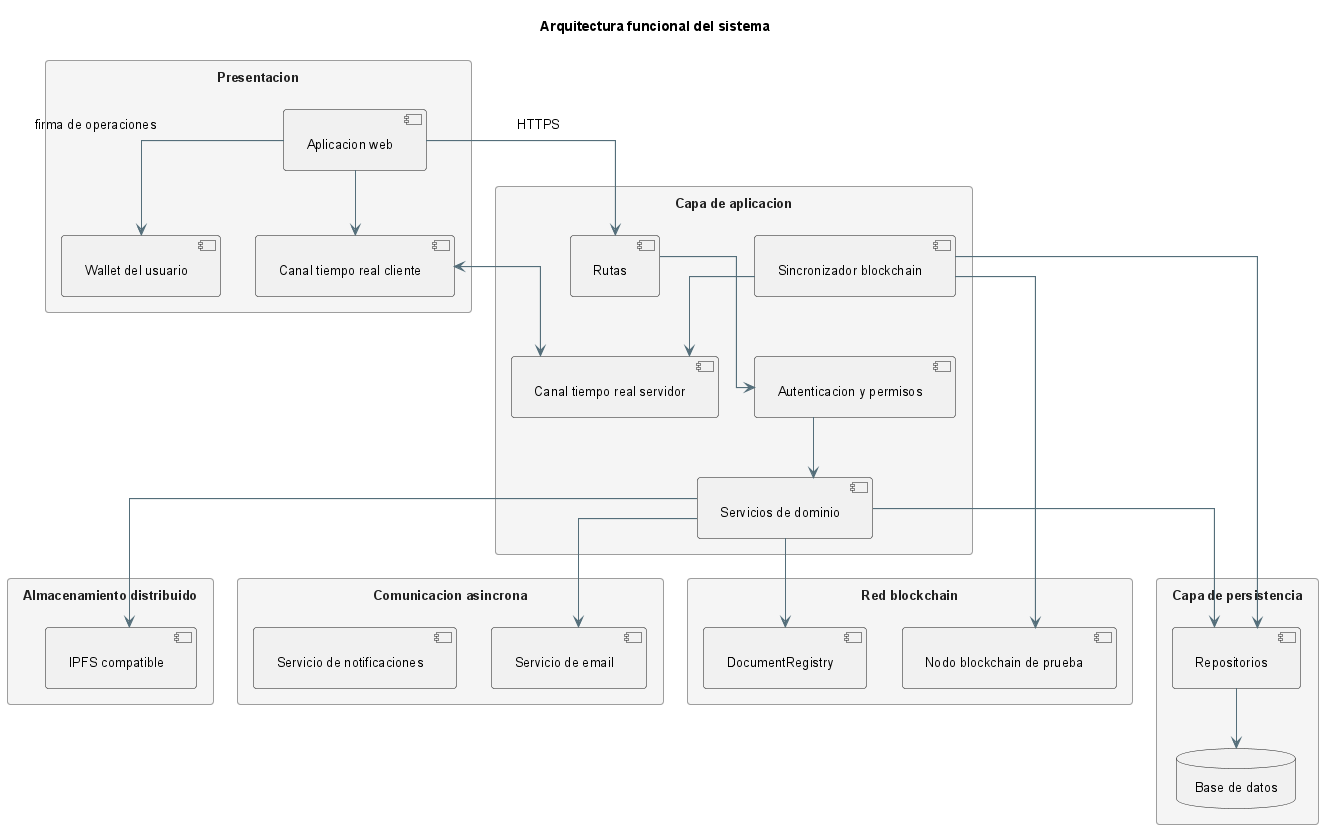
\includegraphics[width=0.95\textwidth]{diagramas/arquitectura.png}
    \caption{Arquitectura general del sistema DocumentChain}
    \label{fig:arquitectura-general}
\end{figure}

\subsection{Subsistemas principales}

El frontend constituye la capa visible para usuarios y administradores. Desde esa interfaz se realizan operaciones de autenticación, carga documental, consulta, firma, compartición y administración. El backend coordina validación, cifrado, almacenamiento, sincronización blockchain, notificaciones y recuperación de evidencias. PostgreSQL mantiene el estado de trabajo necesario para la aplicación. IPFS conserva el binario. El contrato \texttt{DocumentRegistry} opera como capa verificable de autoría, permisos y eventos críticos.

\begin{table}[H]
    \centering
    \small
    \begin{tabular}{|p{3.3cm}|p{3.9cm}|p{6.5cm}|}
    \hline
    \textbf{Subsistema} & \textbf{Base tecnológica} & \textbf{Responsabilidad principal} \\
    \hline
    Frontend web & React, Vite, TypeScript & Navegación, formularios, representación del estado, interacción con wallet y descifrado en cliente. \\
    \hline
    Backend API & Express, Prisma, Node.js & Lógica de negocio, control de acceso, cifrado, integración IPFS y coordinación de confirmaciones blockchain. \\
    \hline
    Persistencia relacional & PostgreSQL & Usuarios, sesiones, carpetas, notificaciones y proyecciones de consulta. \\
    \hline
    Almacenamiento documental & IPFS con nodo Kubo autoalojado & Conservación del binario, generación de CID y soporte de documentos públicos o privados. \\
    \hline
    Evidencia compartida & Hardhat, Solidity, Ethers & Registro verificable de versiones, permisos, firmas y cambios de propiedad. \\
    \hline
    \end{tabular}
    \caption{Subsistemas principales y su responsabilidad dentro de la solución}
    \label{tab:subsistemas-solucion}
\end{table}

\subsection{Gestión de identidad y acceso}

La solución propuesta distingue con claridad entre identidad de cuenta e identidad de firma. El acceso ordinario a la plataforma se apoya en credenciales tradicionales reforzables con segundo factor, lo que favorece una experiencia de uso estable para las tareas habituales. La wallet aparece solo cuando una operación debe dejar rastro \textit{on-chain} y, por tanto, requiere una autorización no delegable. Esta separación mejora la usabilidad y, al mismo tiempo, conserva el valor probatorio de la firma blockchain.

El registro de cuenta se realiza mediante un formulario que solicita nombre de usuario, correo electrónico y contraseña. Tras la alta, el sistema presenta la \textit{Recovery Key}, muestra una confirmación de alta y envía un correo de verificación que el usuario debe confirmar antes del primer acceso ordinario. La entrada al área autenticada queda bloqueada hasta que el campo \texttt{emailVerified} pasa a estado confirmado. La Figura~\ref{fig:register-mem} muestra el formulario de creación de cuenta.

\begin{figure}[H]
    \centering
    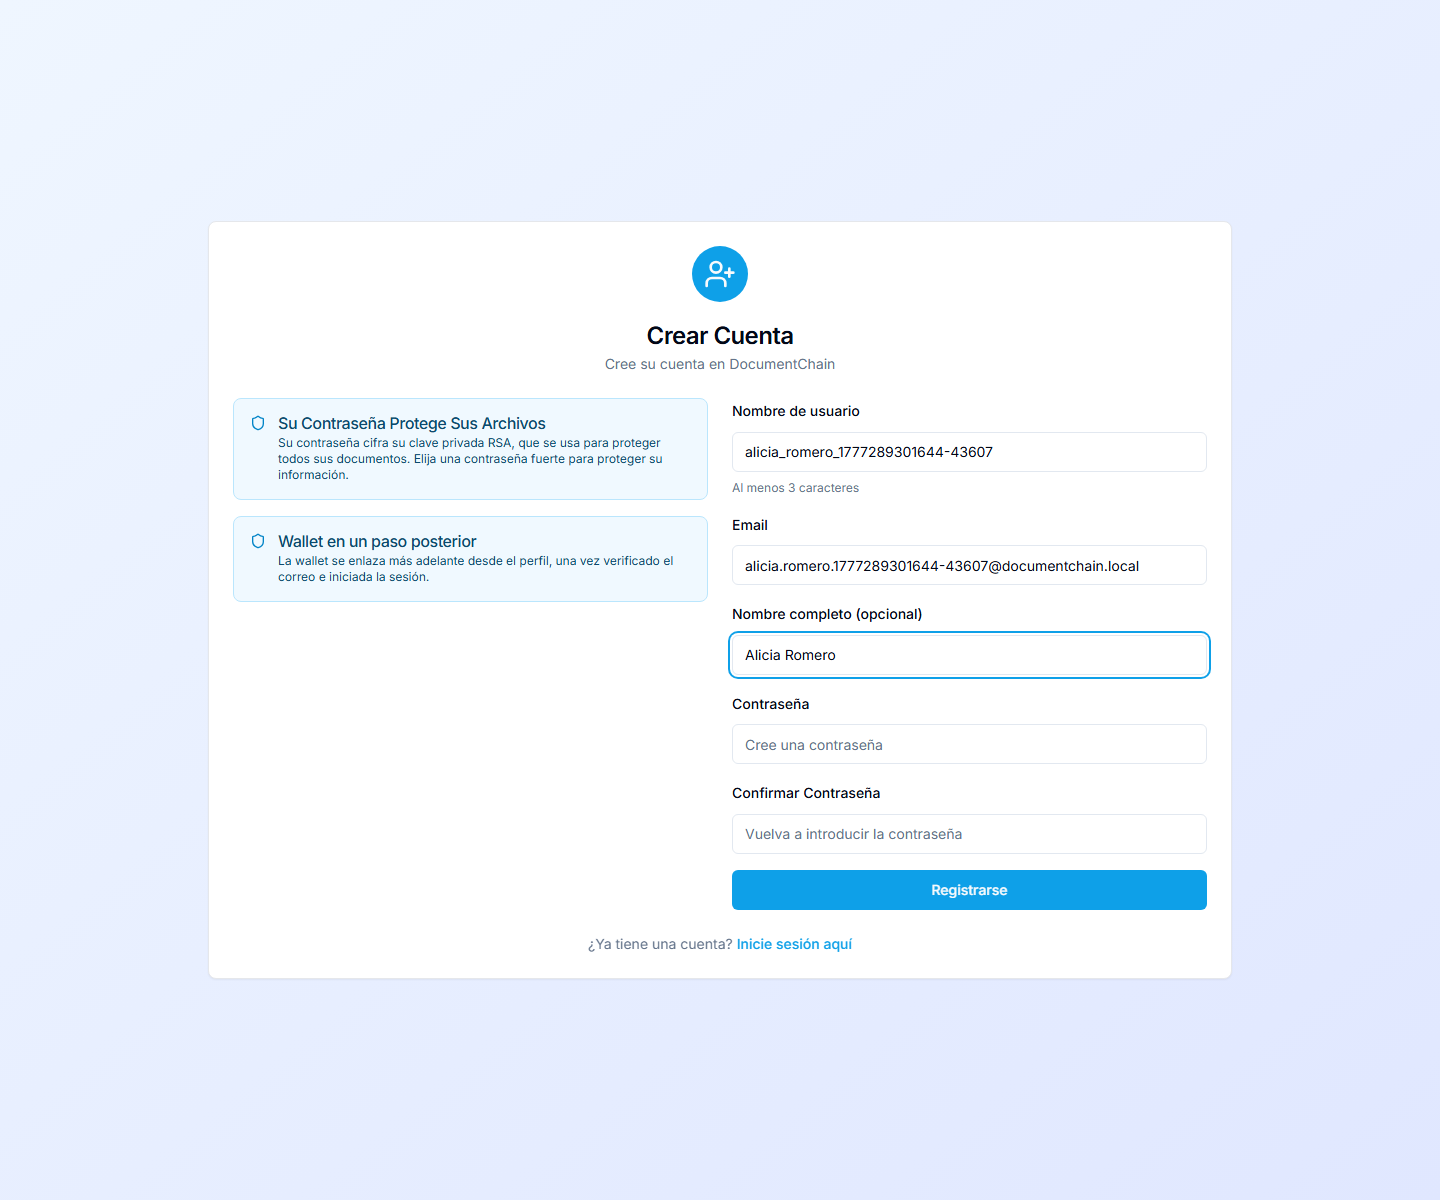
\includegraphics[width=0.88\textwidth]{capturas-ui/register-form.png}
    \caption{Formulario de registro de nuevo usuario con validación de campos}
    \label{fig:register-mem}
\end{figure}

La autenticación con segundo factor se activa de forma opcional desde la sección de configuración de seguridad. El sistema genera un código QR que el usuario vincula a una aplicación TOTP. La Figura~\ref{fig:2fa-setup-mem} muestra el proceso de configuración.

\begin{figure}[H]
    \centering
    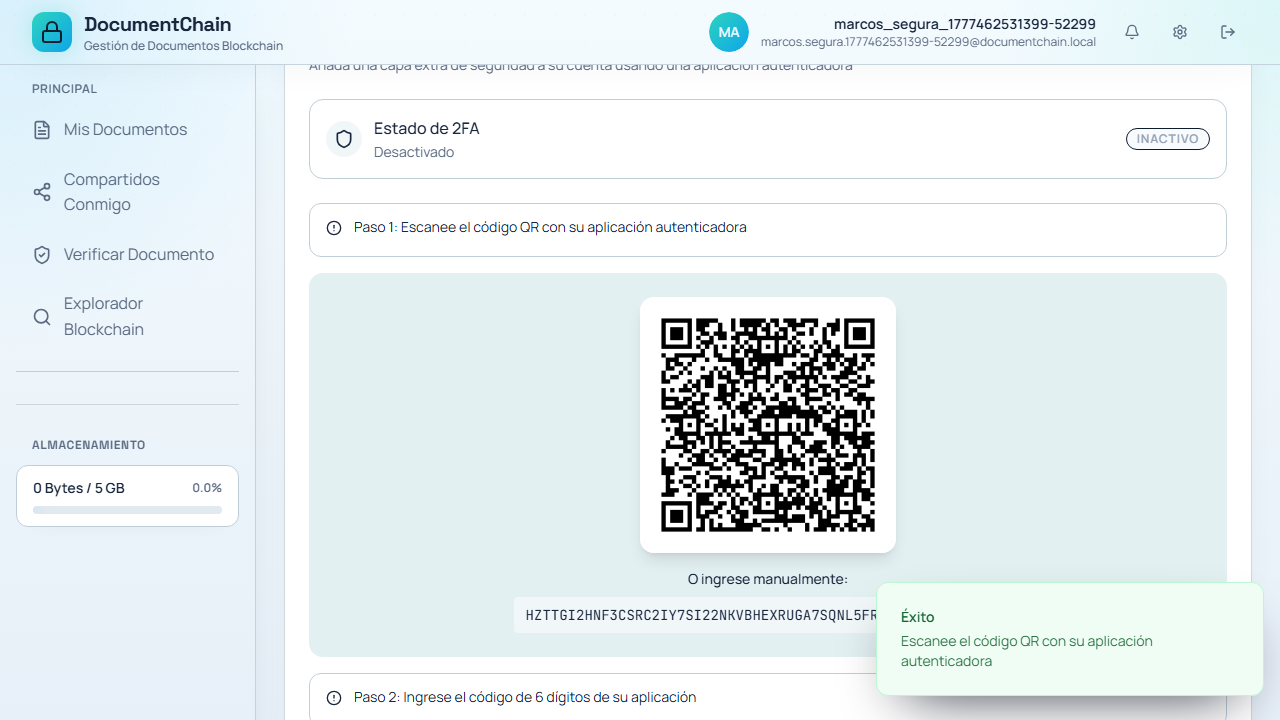
\includegraphics[width=0.88\textwidth]{capturas-ui/two-factor-setup.png}
    \caption{Configuración del segundo factor TOTP desde el perfil de seguridad}
    \label{fig:2fa-setup-mem}
\end{figure}

Una vez activado el 2FA, el inicio de sesión solicita el código de verificación en un segundo paso, tal como muestra la Figura~\ref{fig:2fa-login-mem}.

\begin{figure}[H]
    \centering
    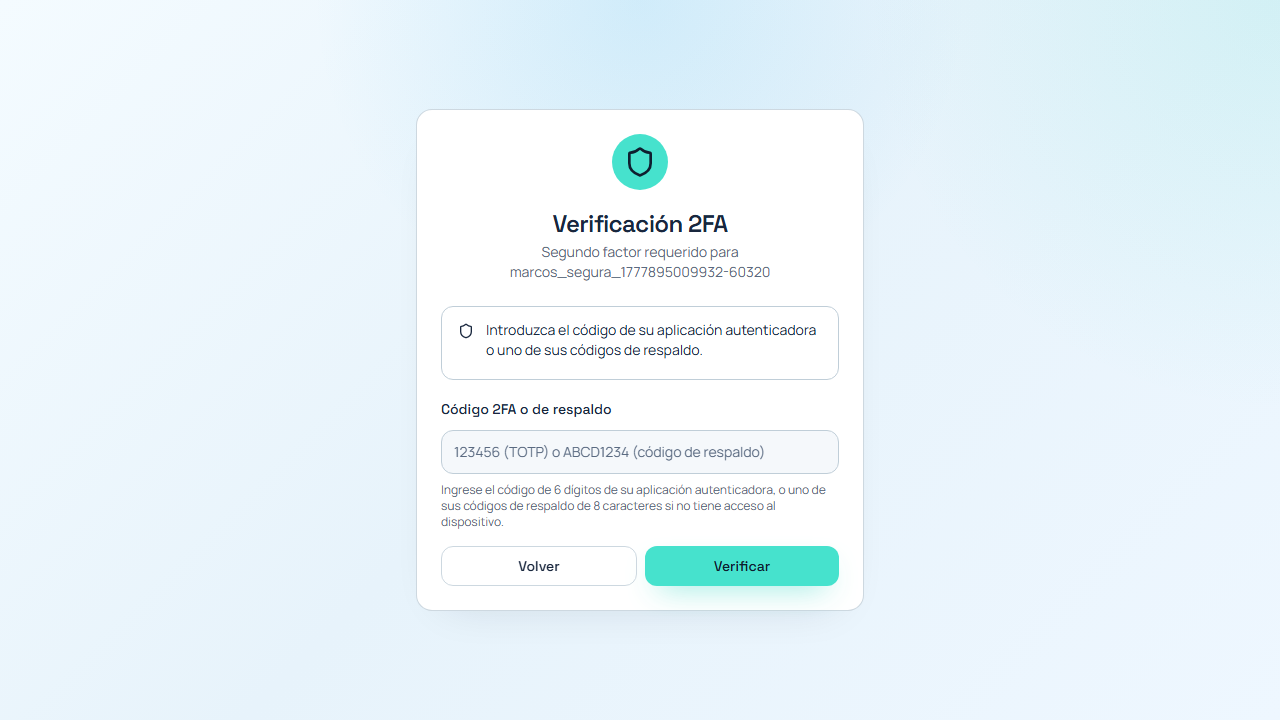
\includegraphics[width=0.88\textwidth]{capturas-ui/two-factor-login.png}
    \caption{Pantalla de verificación del segundo factor durante el inicio de sesión}
    \label{fig:2fa-login-mem}
\end{figure}

La gestión de wallets permite asociar una o varias wallets Ethereum a la cuenta. La Figura~\ref{fig:wallet-sel-mem} muestra el selector de wallet que aparece cuando una operación requiere firma blockchain.

\begin{figure}[H]
    \centering
    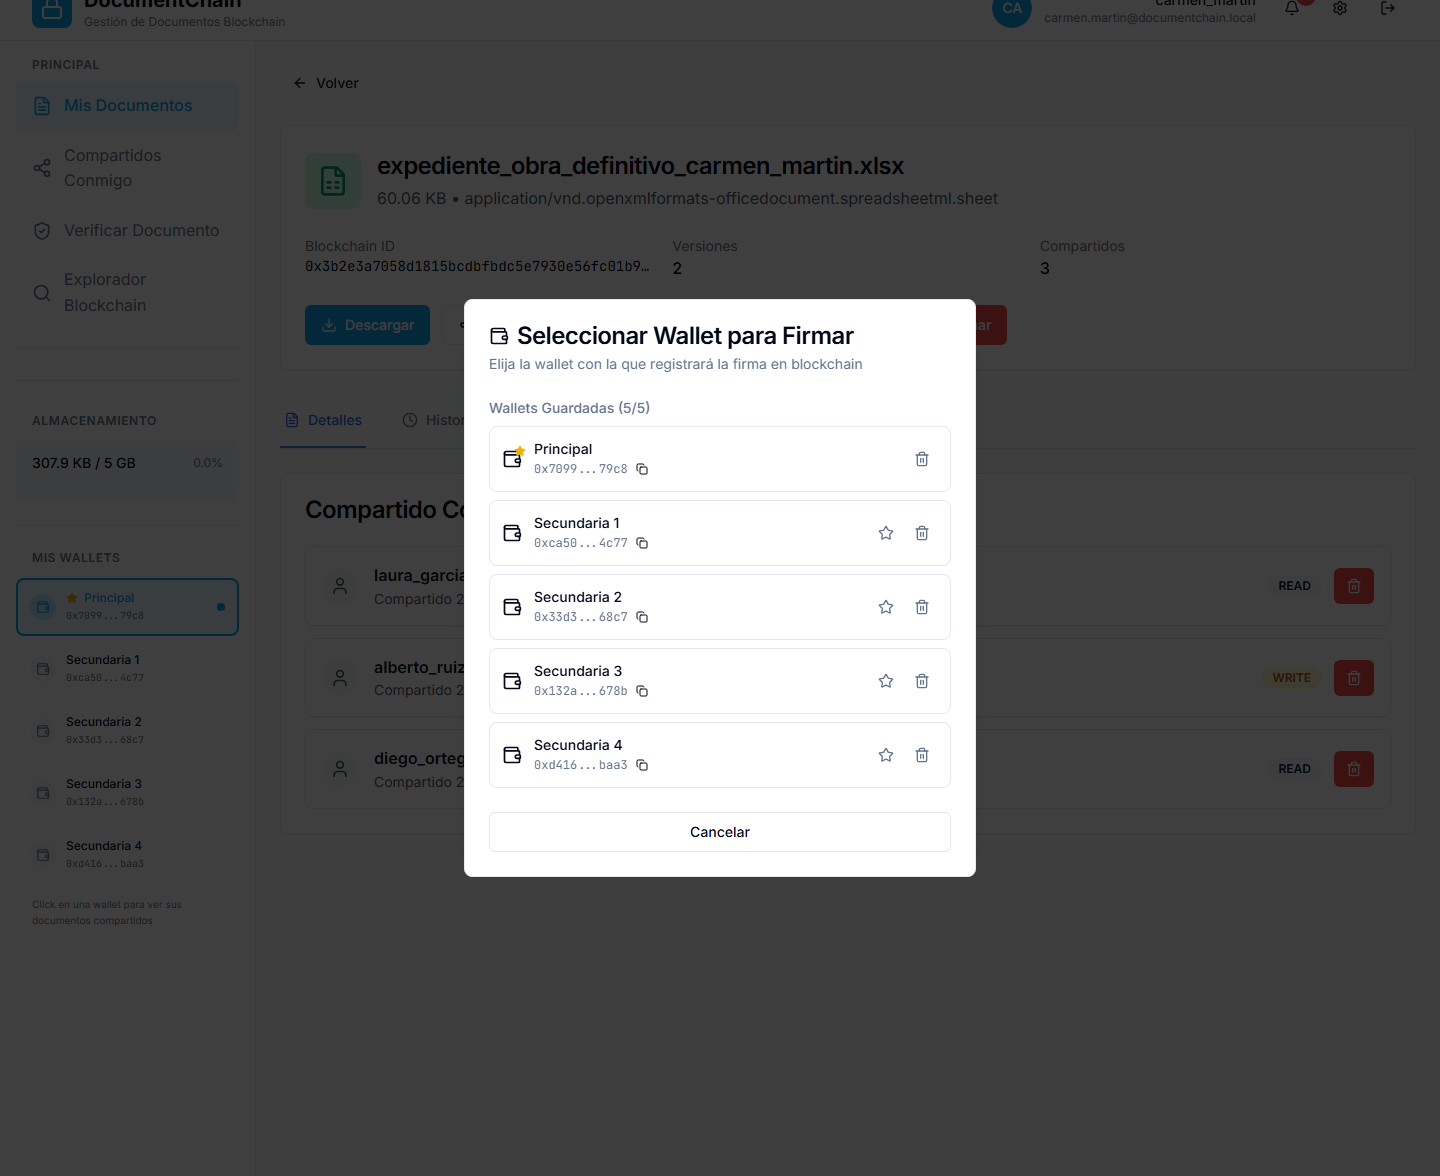
\includegraphics[width=0.78\textwidth]{capturas-ui/wallet-selector-modal.png}
    \caption{Modal de selección de wallet para operaciones que requieren firma on-chain}
    \label{fig:wallet-sel-mem}
\end{figure}

El modelo de acceso se completa con permisos documentales granulares y con una capa administrativa separada. No todos los usuarios participan del mismo modo en el sistema: el propietario concentra la gestión de sus documentos, los usuarios compartidos actúan según rol recibido, y los administradores operan sobre métricas globales, actividad y cuentas.

\subsection{Ciclo de vida del documento}

El núcleo de la solución se articula alrededor del ciclo de vida documental. Un documento puede nacer como privado o público, incorporar nuevas versiones, cambiar su versión operativa, compartirse con terceros, firmarse, archivarse, reactivarse o transferirse a otro usuario. Cada una de estas transiciones conserva una dimensión operativa en PostgreSQL y, cuando corresponde, una dimensión verificable en blockchain. IPFS actúa como soporte del contenido asociado a cada versión.

El listado principal de documentos ofrece filtrado por carpeta y búsqueda textual, con opción de incluir documentos archivados. La Figura~\ref{fig:docs-page-mem} muestra el estado del panel documental con varios documentos.

\begin{figure}[H]
    \centering
    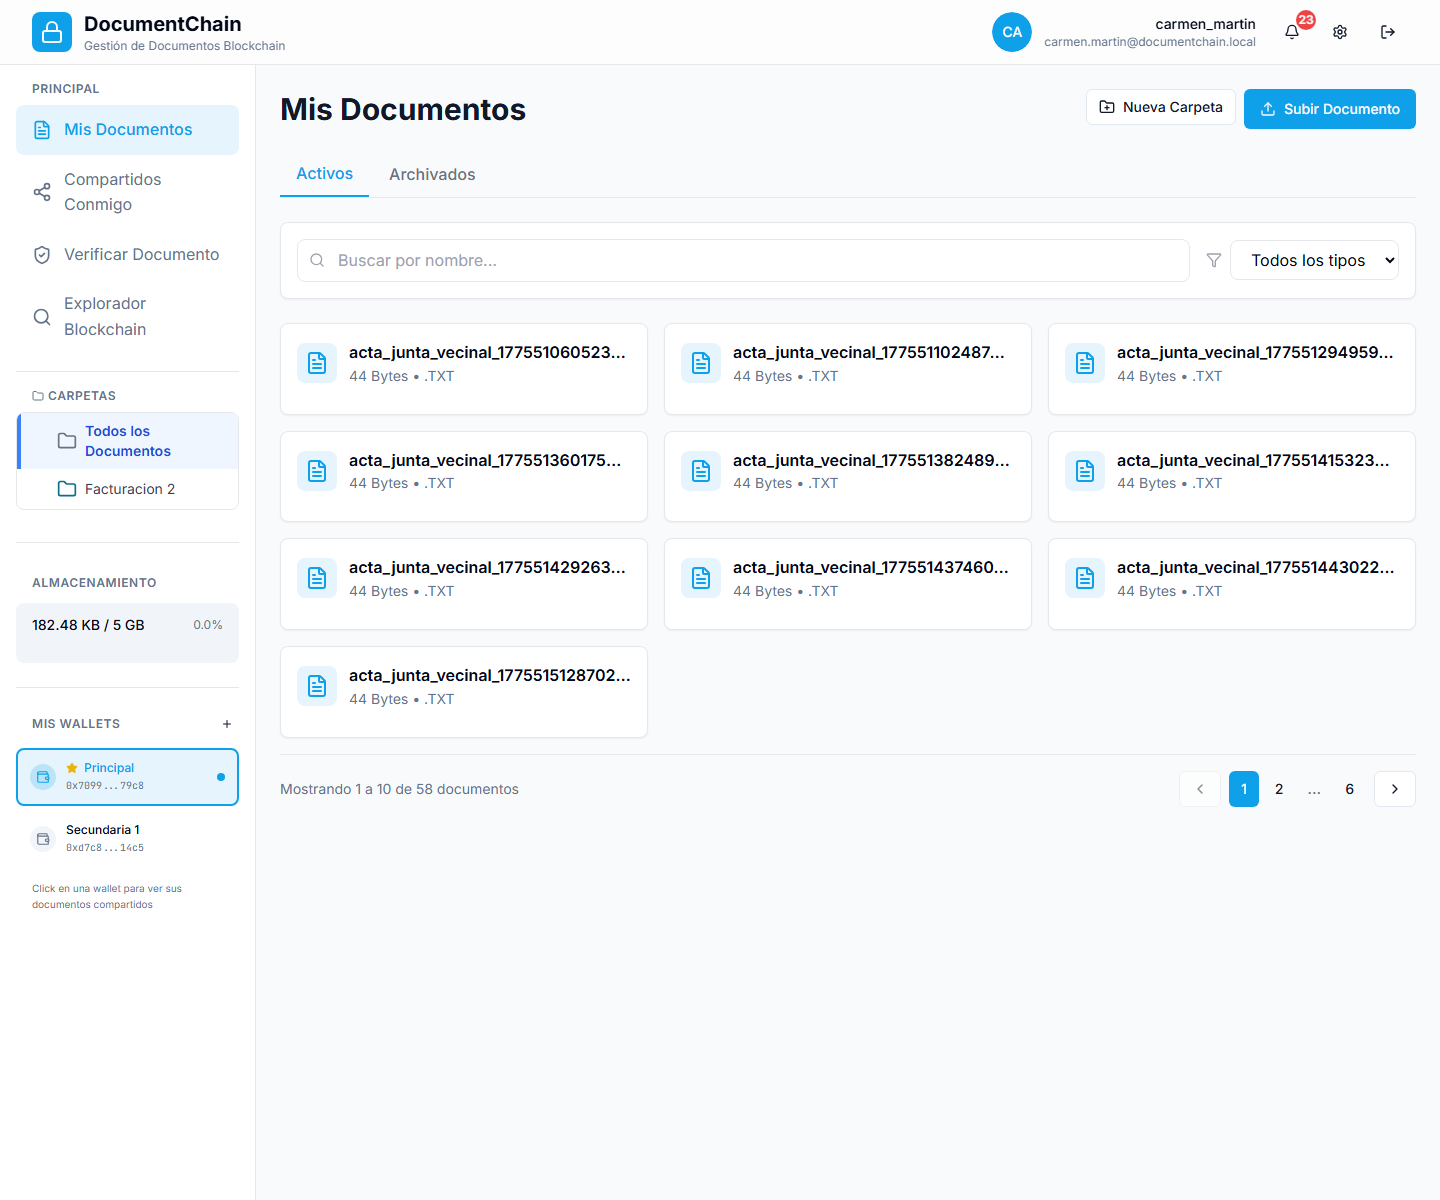
\includegraphics[width=0.92\textwidth]{capturas-ui/documents-page.png}
    \caption{Panel principal de gestión documental con listado, filtros y acceso a detalle}
    \label{fig:docs-page-mem}
\end{figure}

La subida de un nuevo documento se realiza desde un modal que permite configurar todos los atributos relevantes, incluido el tipo de visibilidad. La Figura~\ref{fig:upload-modal-mem} muestra ese formulario de alta.

\begin{figure}[H]
    \centering
    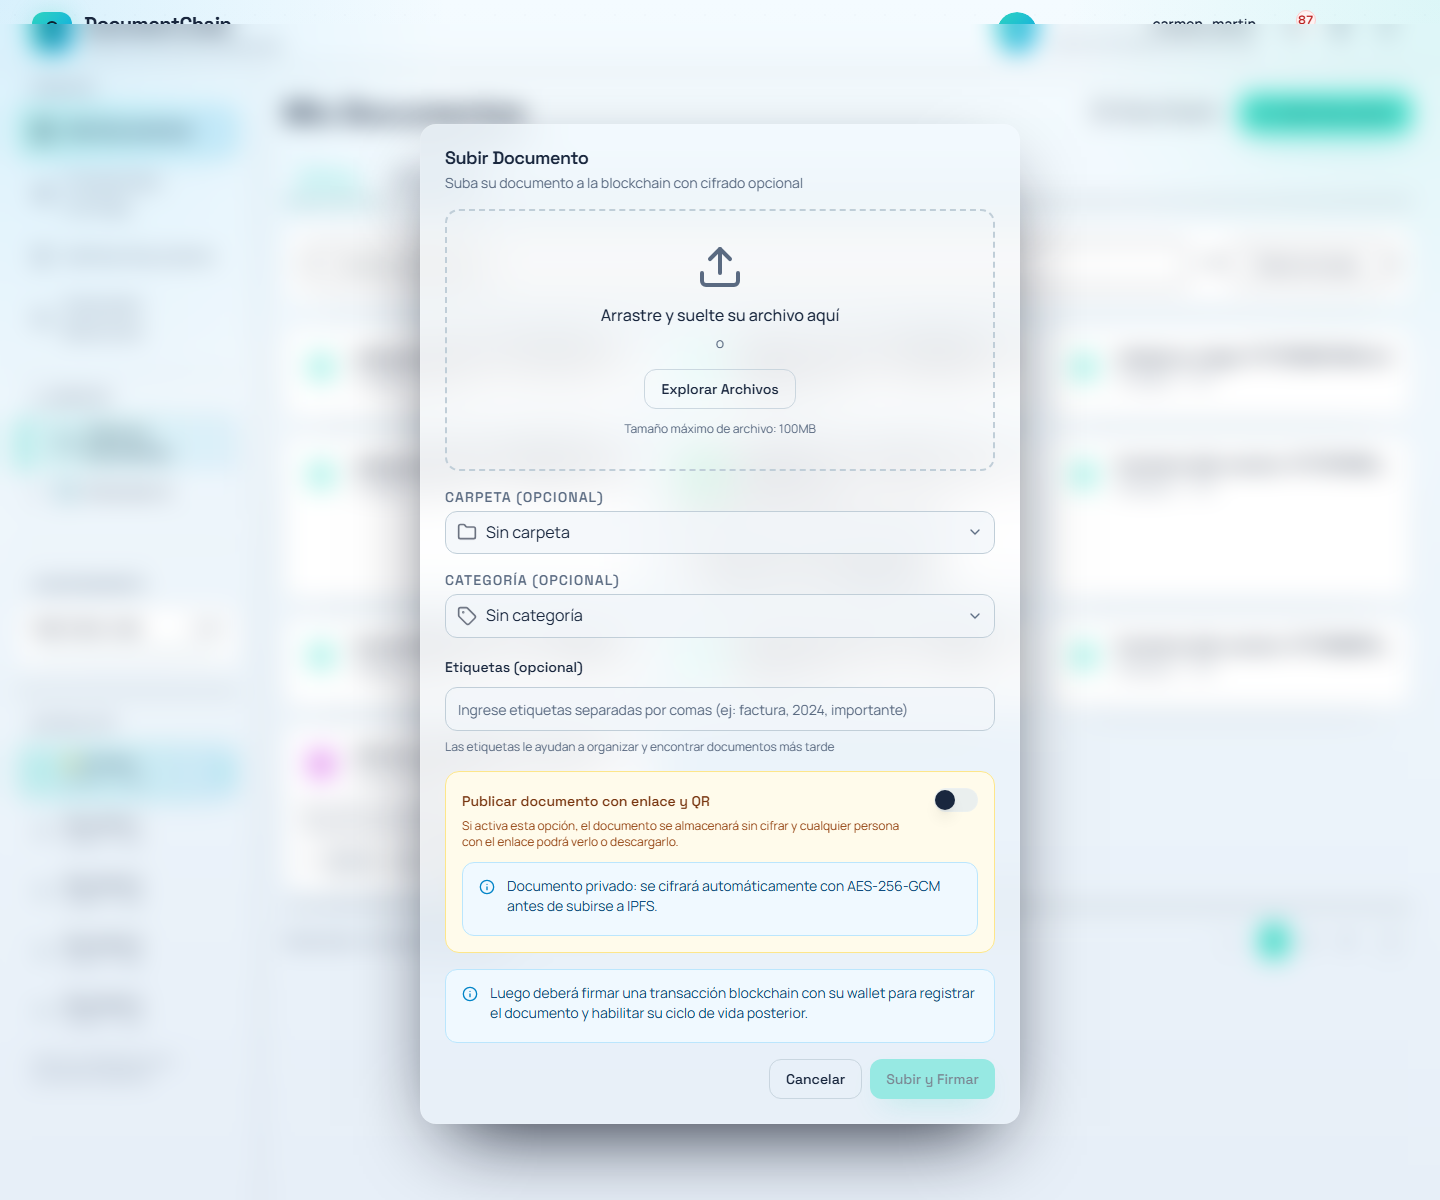
\includegraphics[width=0.87\textwidth]{capturas-ui/upload-modal.png}
    \caption{Modal de subida de nuevo documento con opciones de metadatos y visibilidad}
    \label{fig:upload-modal-mem}
\end{figure}

Desde la vista de detalle el usuario accede a todas las pestañas operativas: versiones, firmas, actividad y permisos. La Figura~\ref{fig:doc-detail-mem} muestra esa vista.

\begin{figure}[H]
    \centering
    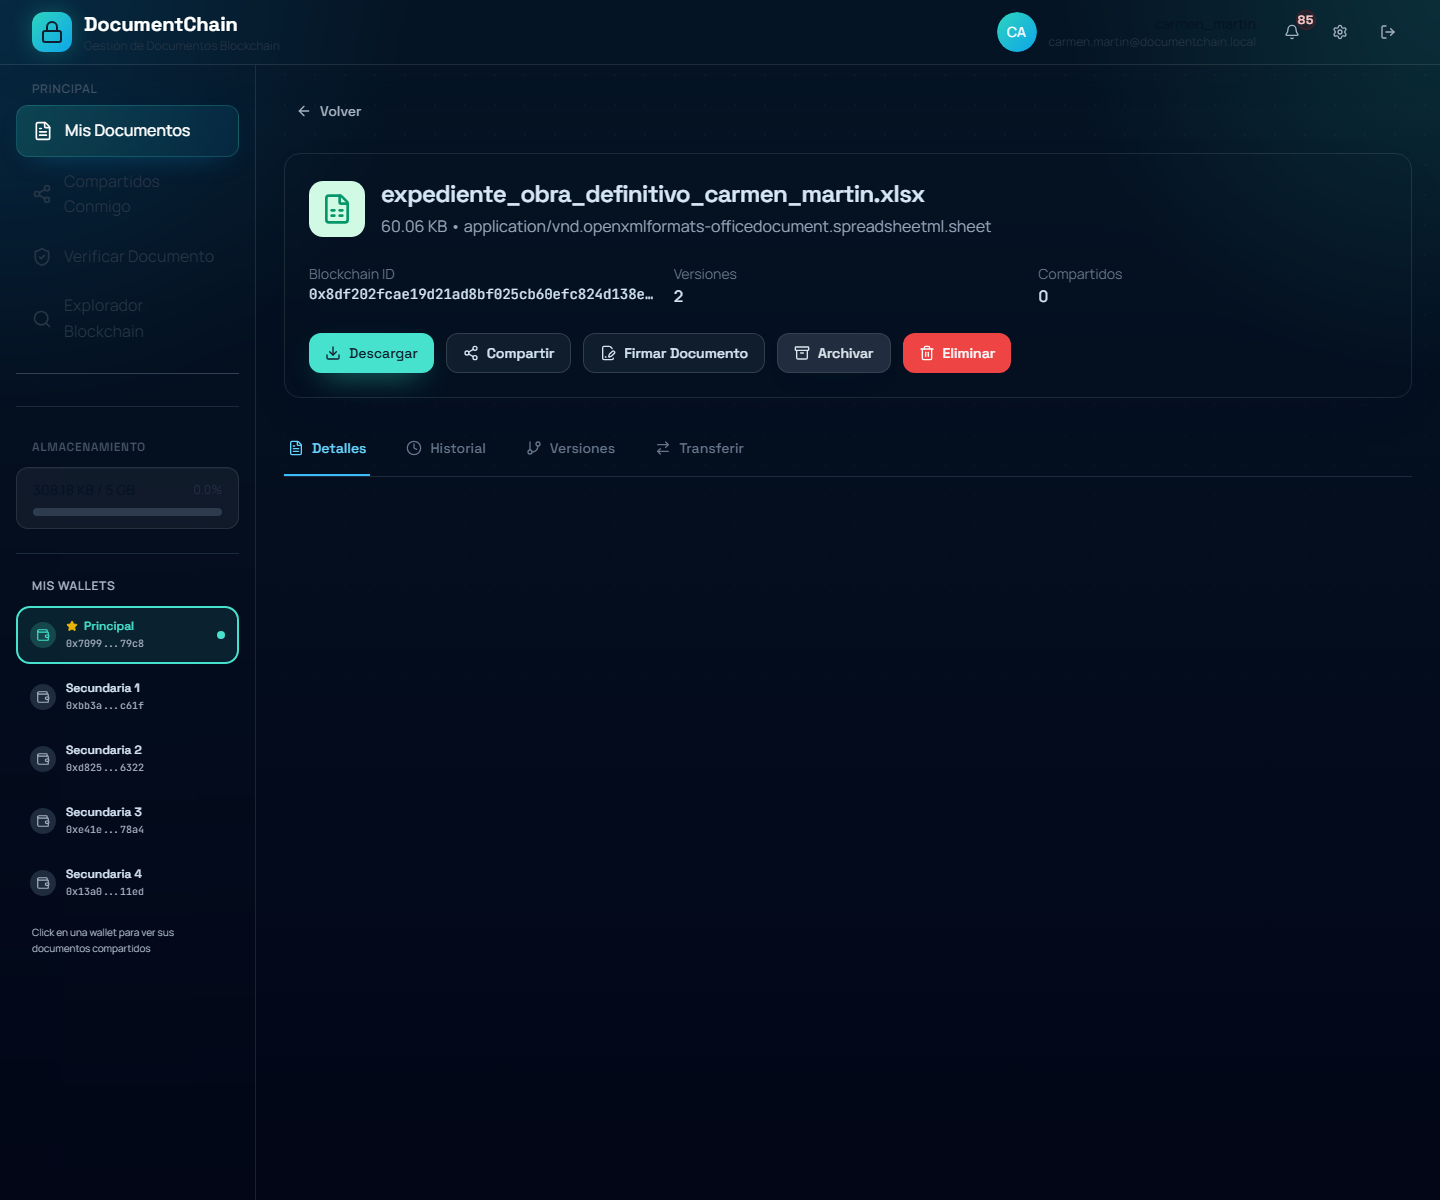
\includegraphics[width=0.92\textwidth]{capturas-ui/document-detail.png}
    \caption{Vista de detalle documental con pestañas de versiones, firmas y metadatos}
    \label{fig:doc-detail-mem}
\end{figure}

La pestaña de versiones permite consultar el historial, activar una versión específica como operativa o subir una nueva versión que sustituya a la actual. La Figura~\ref{fig:versions-mem} muestra el historial de versiones de un documento.

\begin{figure}[H]
    \centering
    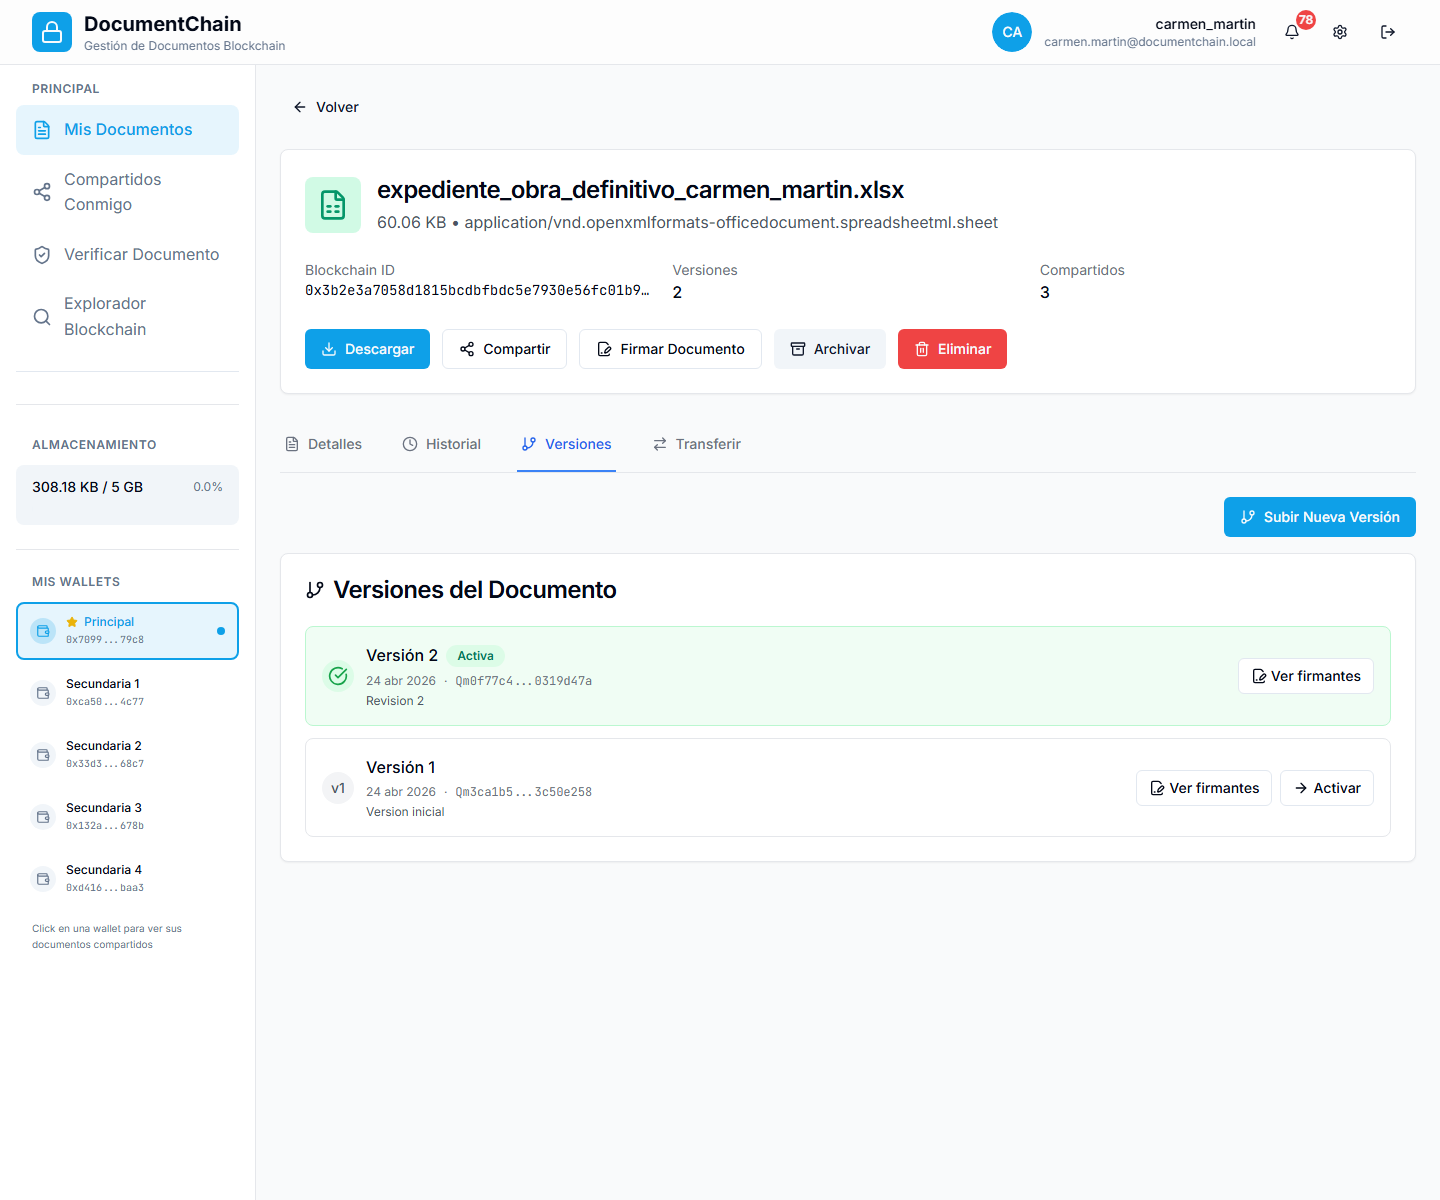
\includegraphics[width=0.92\textwidth]{capturas-ui/versions-tab.png}
    \caption{Pestaña de versiones con historial, CID de IPFS y versión activa marcada}
    \label{fig:versions-mem}
\end{figure}

La subida de una nueva versión se realiza mediante un modal específico que incluye un campo de descripción del cambio y el archivo actualizado. La Figura~\ref{fig:upload-version-mem} ilustra ese proceso.

\begin{figure}[H]
    \centering
    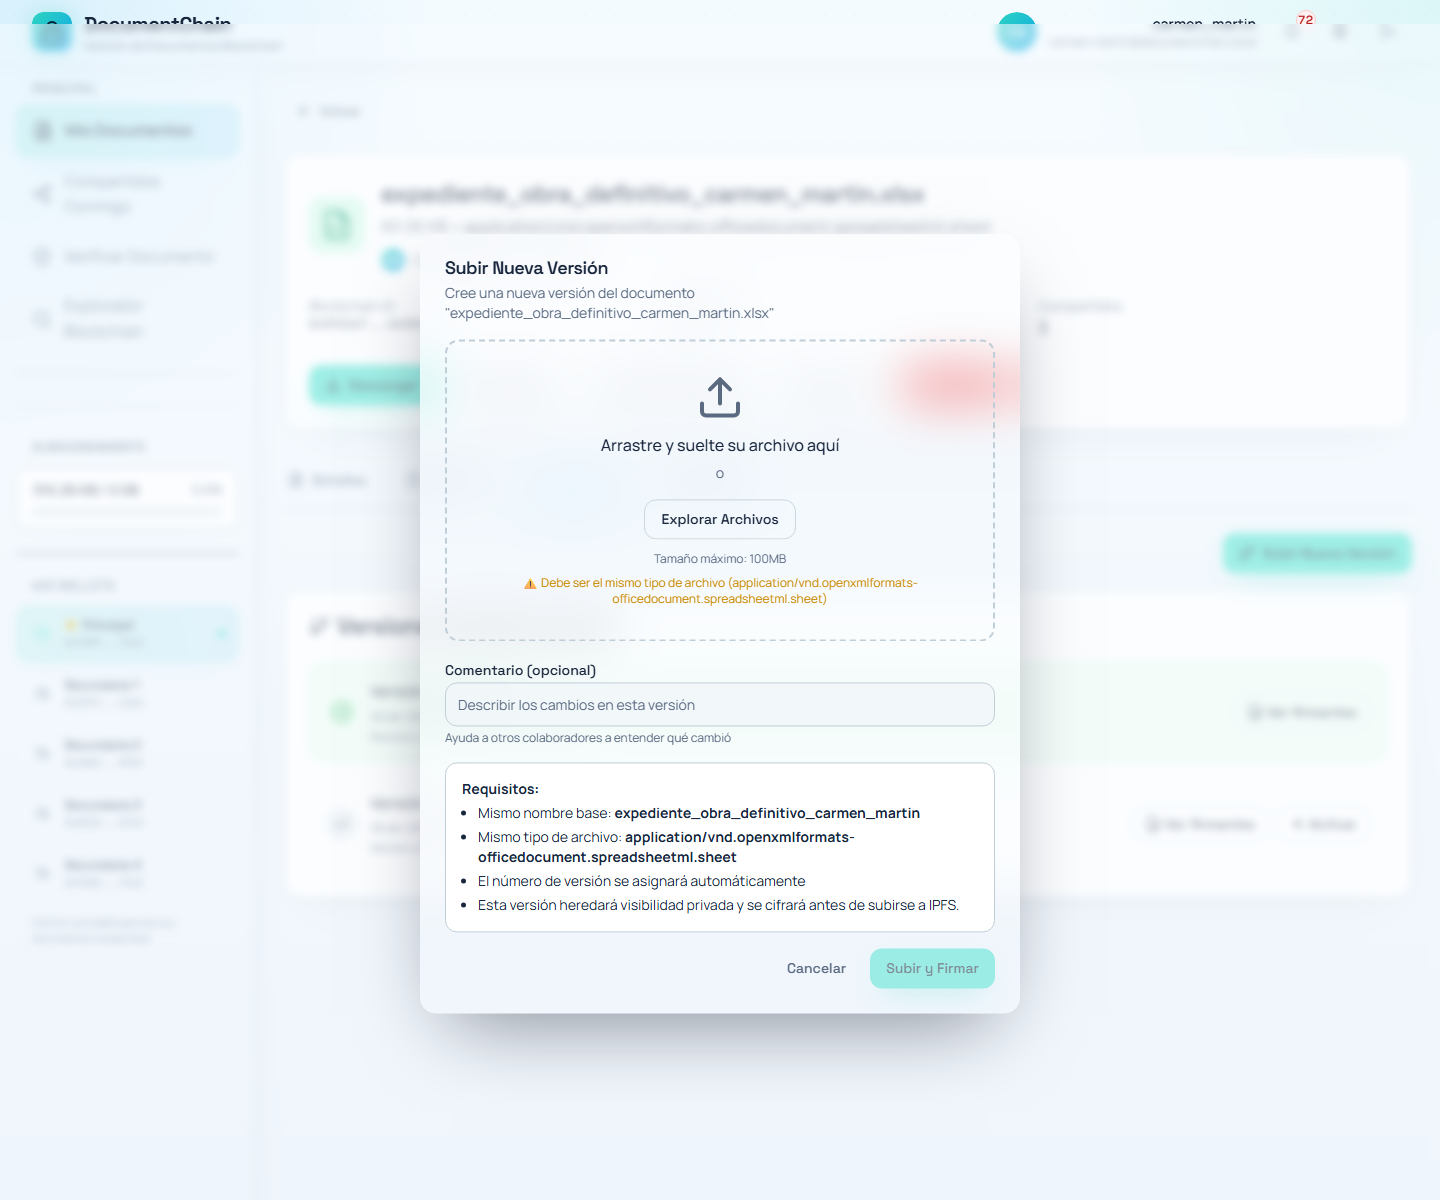
\includegraphics[width=0.82\textwidth]{capturas-ui/upload-version-modal.png}
    \caption{Modal de subida de nueva versión con descripción del cambio}
    \label{fig:upload-version-mem}
\end{figure}

Esta concepción del documento como entidad viva, y no como simple fichero estático, explica buena parte de la complejidad y del interés del proyecto. La plataforma no se limita a subir archivos y listarlos; necesita coordinar estados, permisos, evidencias y accesos públicos o privados sin perder coherencia entre capas.

\subsection{Colaboración, permisos y firma}

La solución incorpora colaboración documental real mediante permisos diferenciados y operaciones de firma. El rol OWNER concentra el control principal sobre el documento, mientras que VIEWER y EDITOR permiten modular consulta y modificación. A ello se suma la posibilidad de revocar accesos o transferir titularidad. En paralelo, la firma digital registrada con wallet introduce una forma de aceptación verificable que no depende solo de un campo interno de base de datos.

La compartición con otro usuario se realiza desde un modal que permite seleccionar destinatario y rol asignado. La Figura~\ref{fig:share-modal-mem} muestra ese diálogo.

\begin{figure}[H]
    \centering
    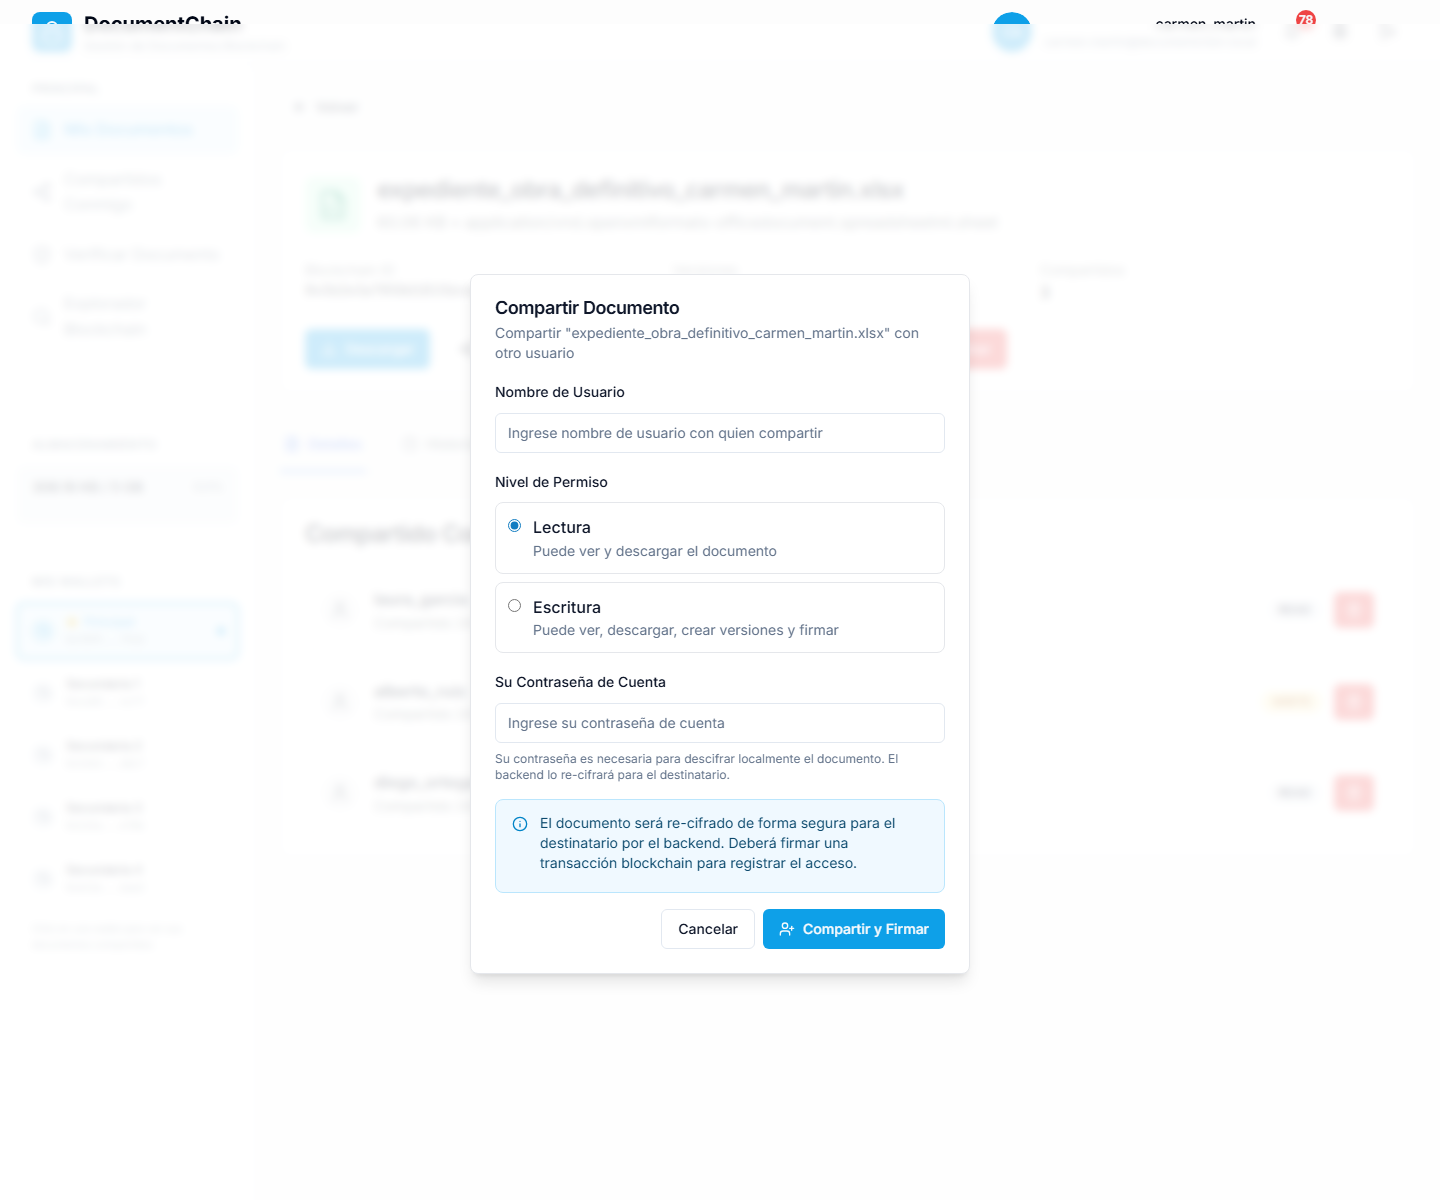
\includegraphics[width=0.78\textwidth]{capturas-ui/share-modal.png}
    \caption{Modal de compartición de documento con selección de usuario y asignación de rol}
    \label{fig:share-modal-mem}
\end{figure}

Los documentos recibidos de otros usuarios aparecen en la sección de documentos compartidos, donde el usuario puede operar según el rol que le ha sido asignado. La Figura~\ref{fig:shared-mem} muestra esa sección.

\begin{figure}[H]
    \centering
    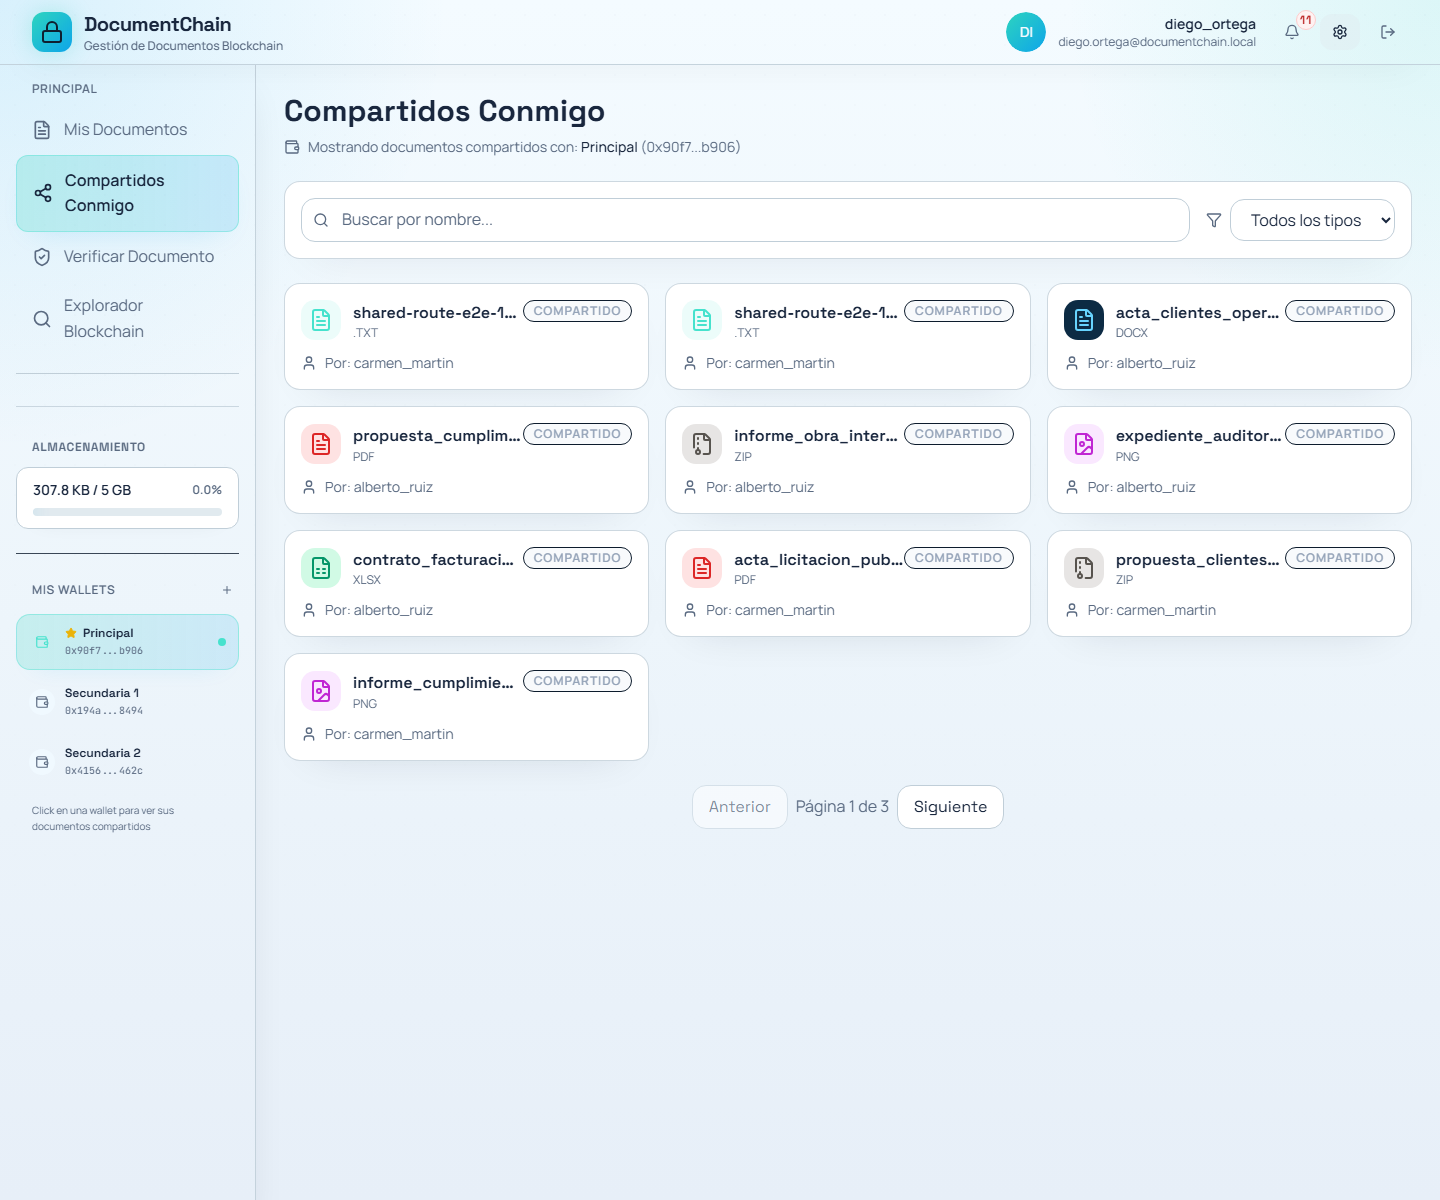
\includegraphics[width=0.92\textwidth]{capturas-ui/shared-page.png}
    \caption{Vista de documentos compartidos con el usuario con indicación del rol recibido}
    \label{fig:shared-mem}
\end{figure}

La firma de un documento requiere wallet activa. El modal de firma permite añadir un comentario opcional, que queda vinculado a la evidencia on-chain. La Figura~\ref{fig:sign-modal-mem} muestra ese proceso.

\begin{figure}[H]
    \centering
    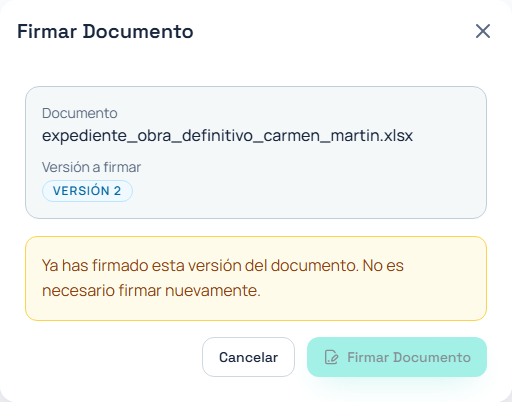
\includegraphics[width=0.78\textwidth]{capturas-ui/sign-modal.png}
    \caption{Modal de firma digital de documento con campo de comentario y botón de confirmación}
    \label{fig:sign-modal-mem}
\end{figure}

La transferencia de propiedad se realiza desde la pestaña de permisos del documento. La Figura~\ref{fig:transfer-mem} muestra la vista de transferencia de titularidad.

\begin{figure}[H]
    \centering
    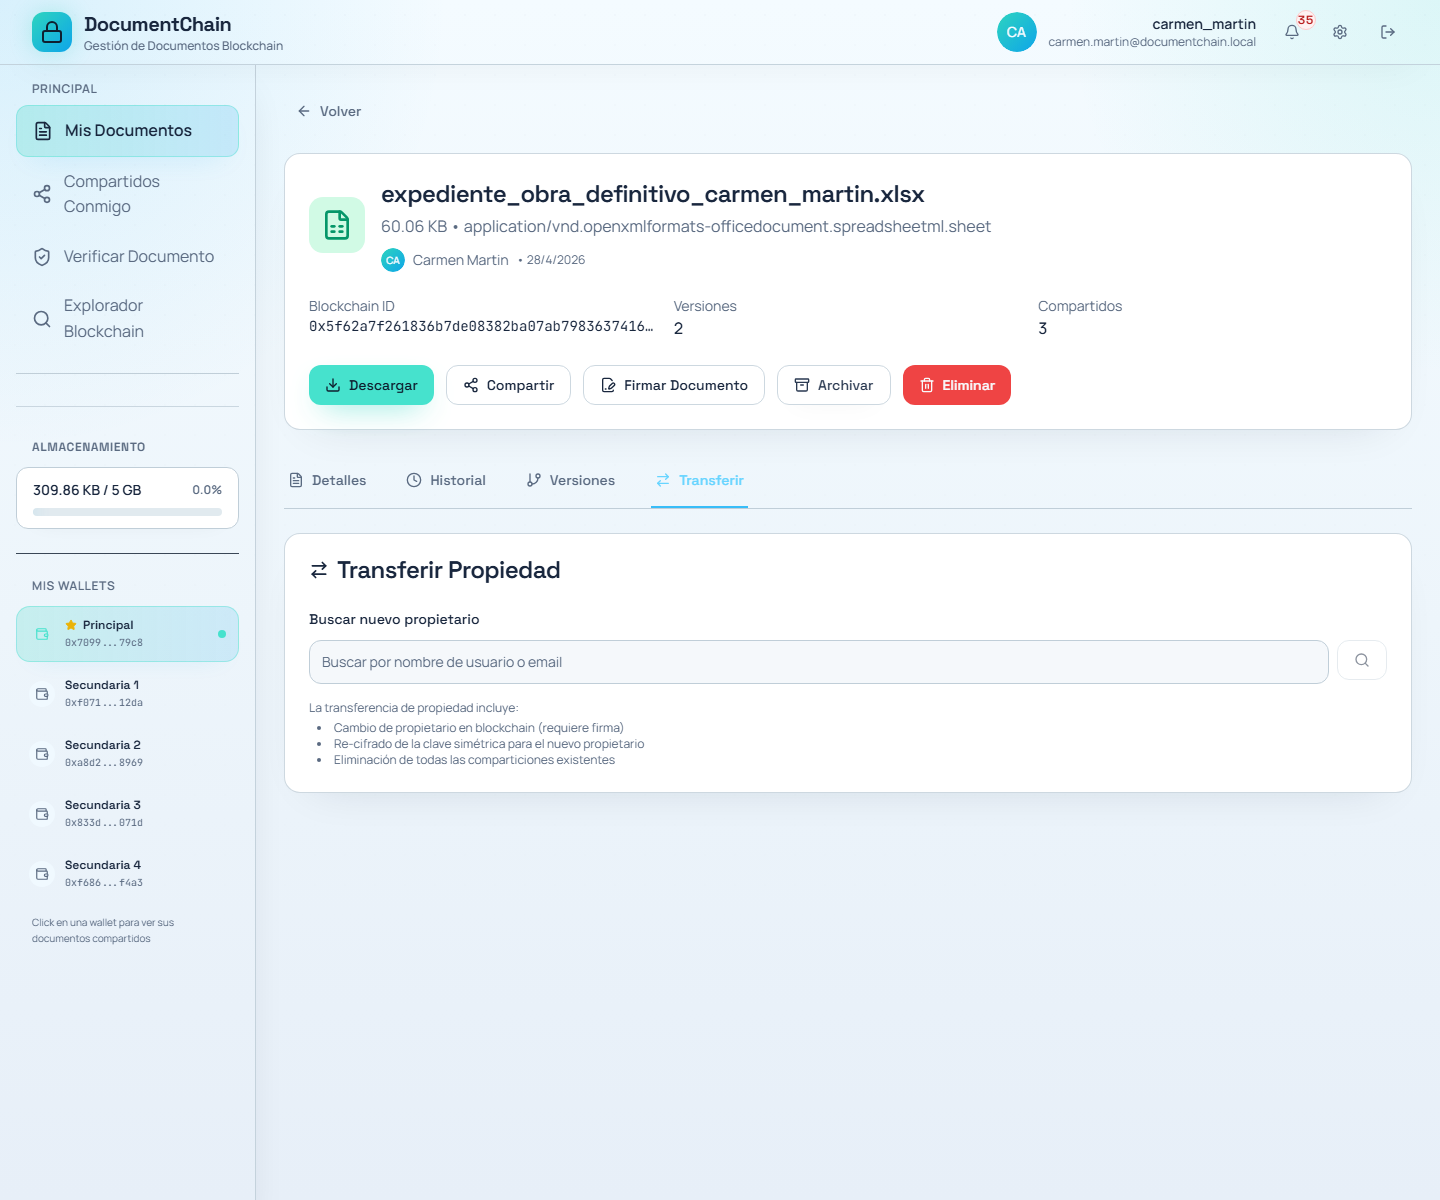
\includegraphics[width=0.88\textwidth]{capturas-ui/transfer-tab.png}
    \caption{Pestaña de transferencia de propiedad del documento a otro usuario}
    \label{fig:transfer-mem}
\end{figure}

Esta combinación amplía el alcance del sistema respecto a un repositorio documental simple. La colaboración deja de ser un mero compartir enlace y pasa a convertirse en un conjunto de relaciones con valor operativo y de trazabilidad.

\subsection{Verificación pública y auditoría}

Una de las aportaciones diferenciales de la solución consiste en ofrecer un plano de verificación accesible sin autenticación para aquellos documentos o evidencias que el usuario ha decidido exponer mediante \texttt{publicId}. Esta decisión permite compatibilizar privacidad por defecto con verificabilidad pública deliberada.

La página de verificación pública permite contrastar la integridad de un documento introduciendo su hash o navegando al enlace público proporcionado. La Figura~\ref{fig:verify-mem} muestra esa vista.

\begin{figure}[H]
    \centering
    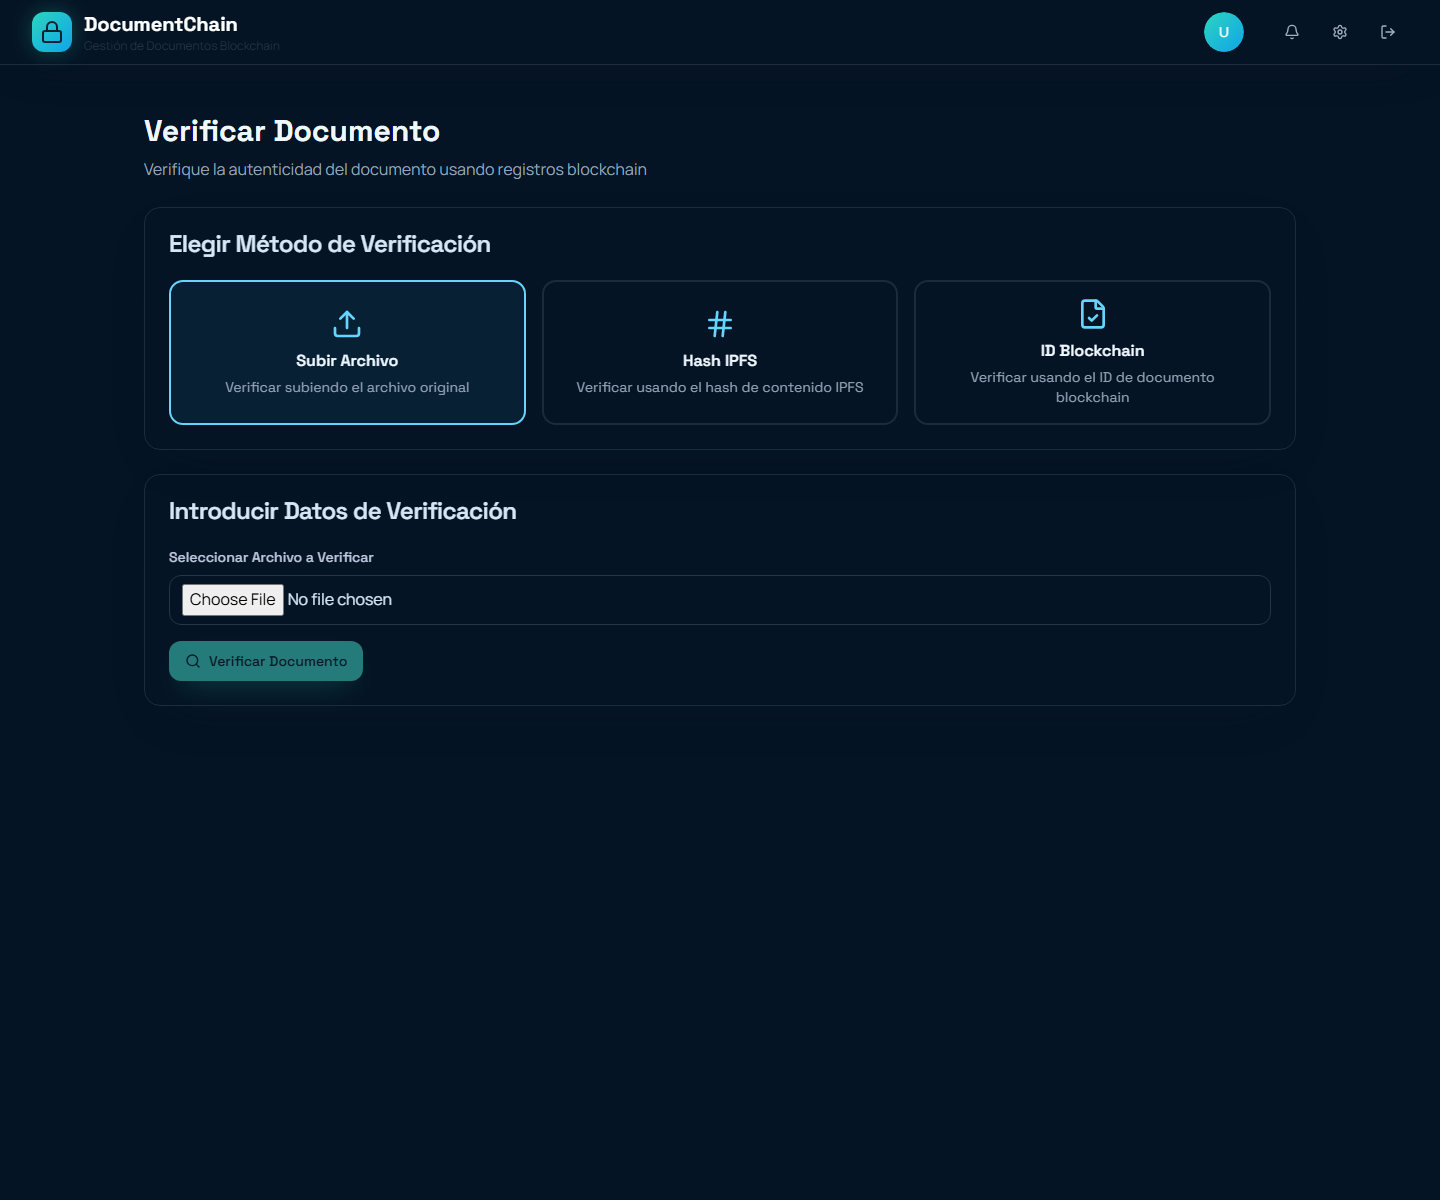
\includegraphics[width=0.90\textwidth]{capturas-ui/verify-page.png}
    \caption{Vista de verificación pública de integridad documental sin autenticación}
    \label{fig:verify-mem}
\end{figure}

La auditoría pública profunda, disponible cuando el propietario la ha habilitado, muestra el historial completo de versiones, firmas y eventos relevantes. La Figura~\ref{fig:audit-mem} muestra esa vista.

\begin{figure}[H]
    \centering
    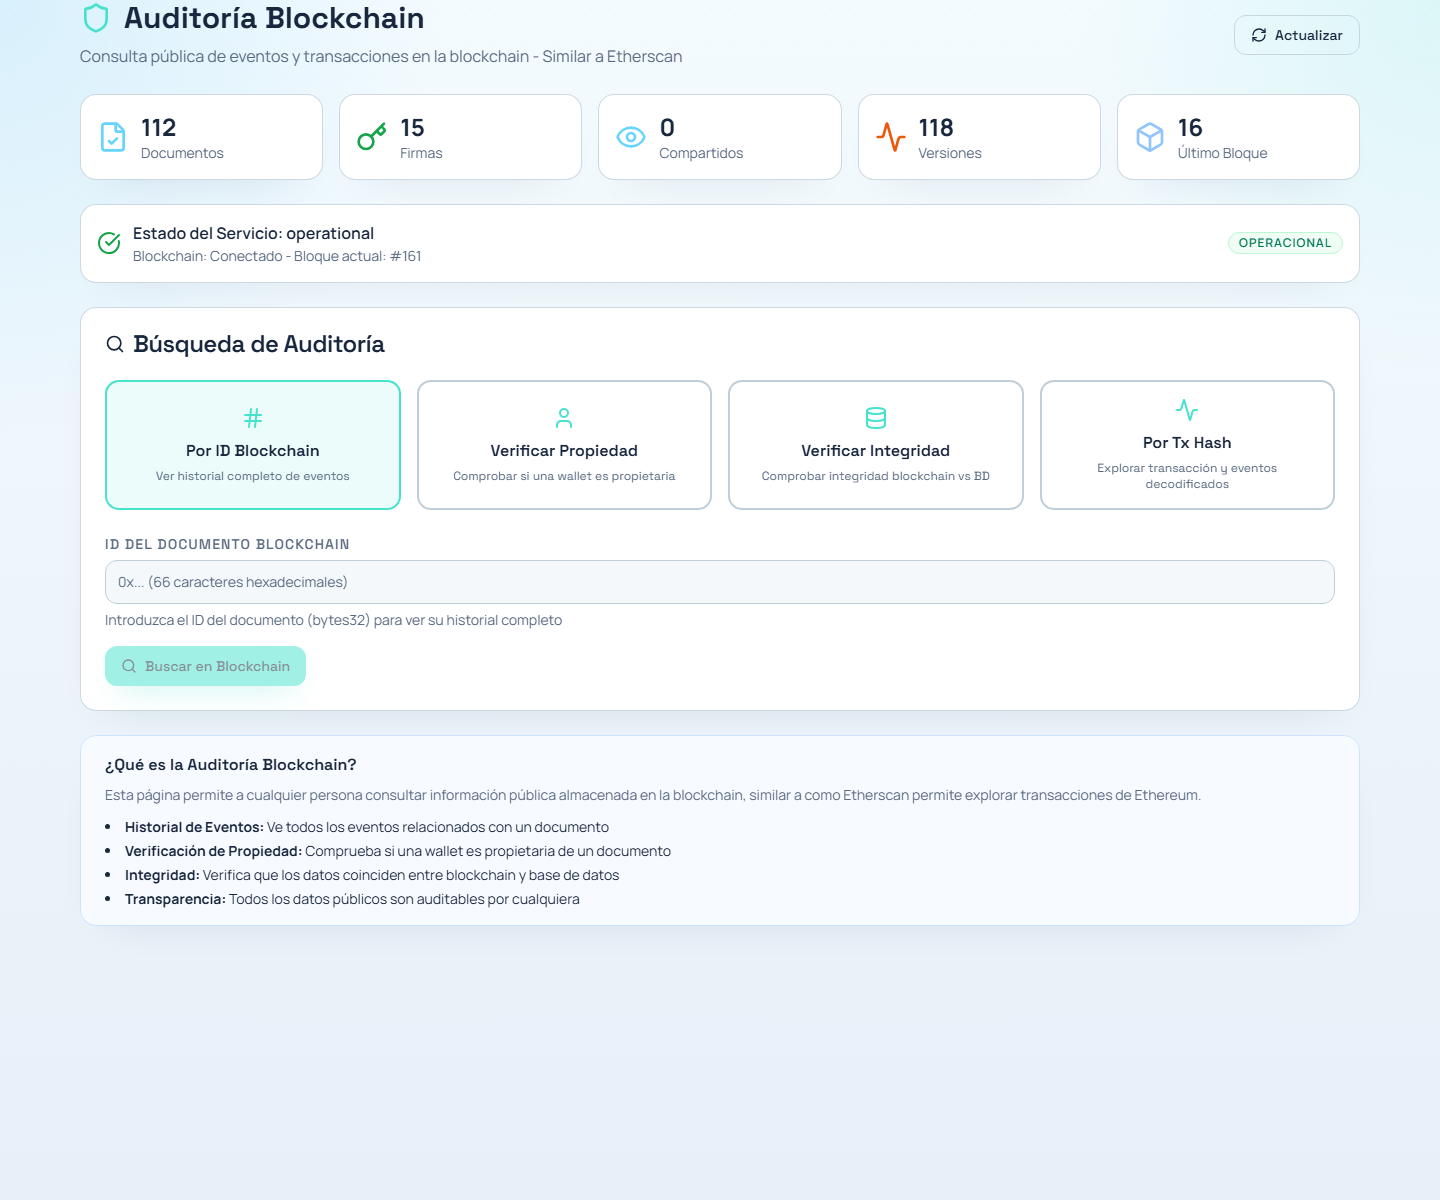
\includegraphics[width=0.90\textwidth]{capturas-ui/public-audit-page.png}
    \caption{Pantalla de auditoría pública con historial completo de eventos verificables}
    \label{fig:audit-mem}
\end{figure}

\subsection{Flujos funcionales representativos}

El comportamiento del sistema puede resumirse en cuatro recorridos especialmente representativos: alta de documento, compartición con terceros, firma digital y verificación pública. En los tres primeros, la aplicación alterna trabajo \textit{off-chain} y firma \textit{on-chain} mediante el patrón \textit{prepare/confirm}. En el cuarto, se expone solo la parte del sistema pensada para comprobación pública, sin trasladar al visitante el resto del estado interno.

El \textit{timeline} de actividad de un documento permite seguir en orden cronológico todos los eventos relevantes del ciclo de vida, incluyendo altas, versiones, firmas y cambios de estado. La Figura~\ref{fig:timeline-mem} muestra esa vista de historial.

\begin{figure}[H]
    \centering
    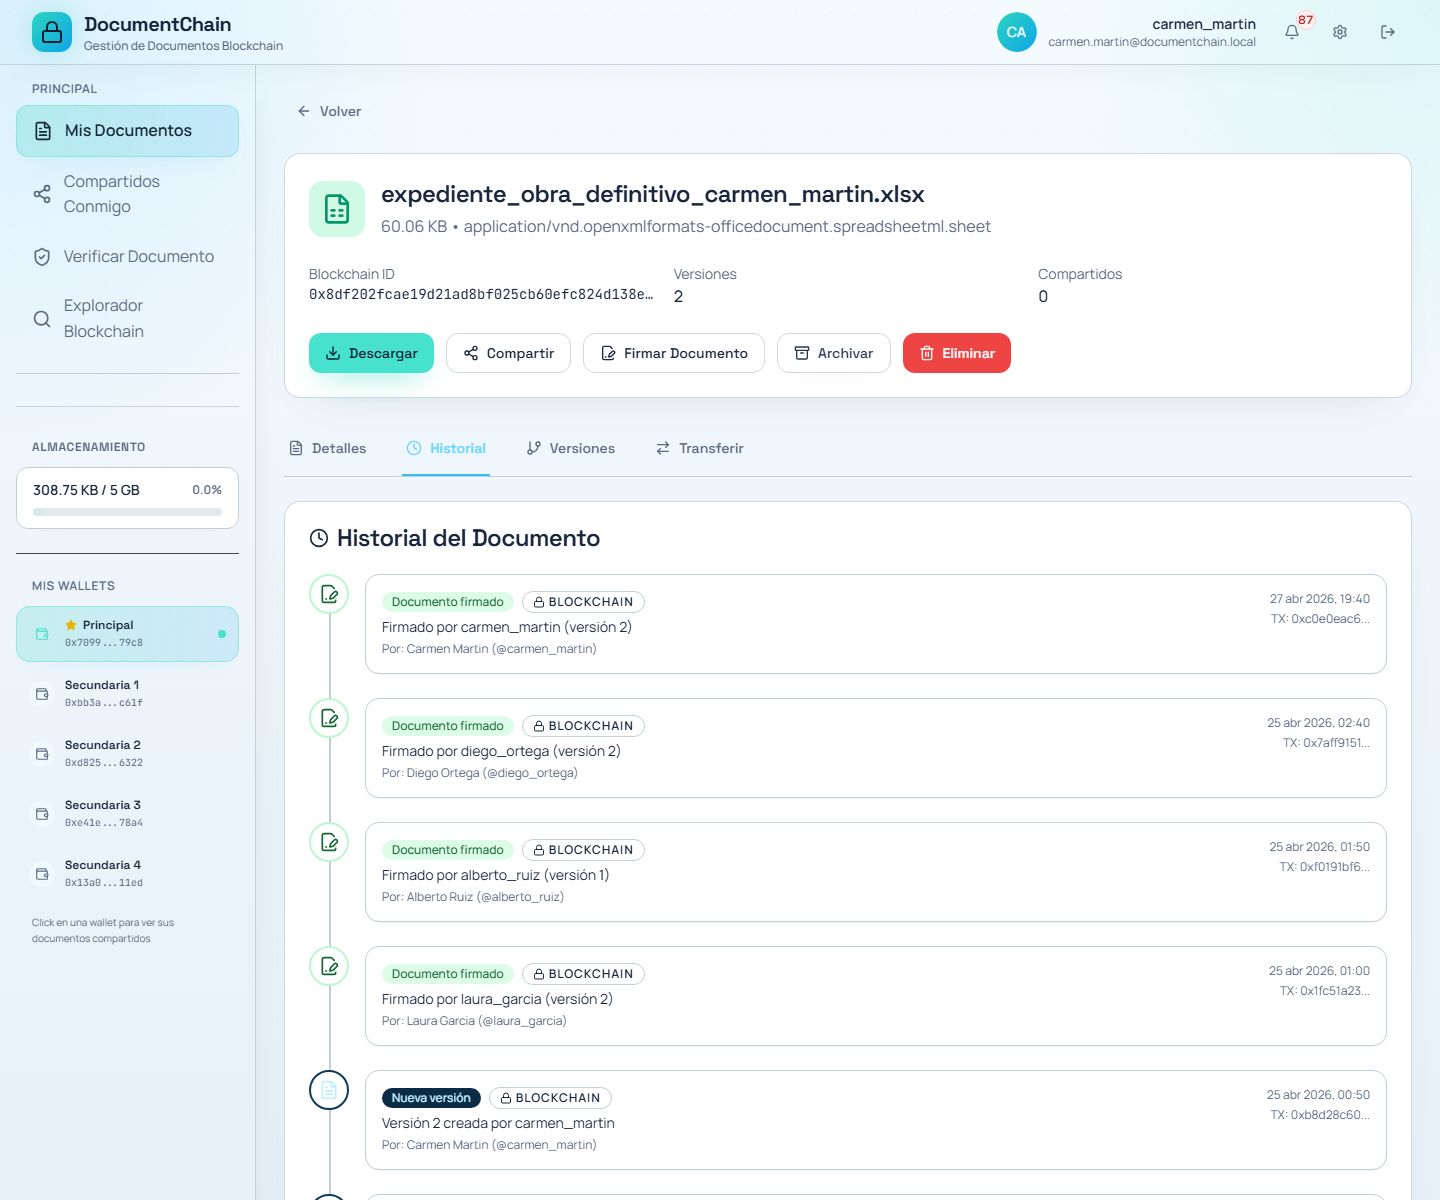
\includegraphics[width=0.92\textwidth]{capturas-ui/timeline-page.png}
    \caption{Timeline de actividad del documento con eventos ordenados cronológicamente}
    \label{fig:timeline-mem}
\end{figure}

\subsection{Notificaciones y comunicación}

El sistema genera notificaciones automáticas asociadas a eventos relevantes: documentos compartidos recibidos, firmas añadidas, versiones subidas por colaboradores, cambios de permisos y transferencias. La Figura~\ref{fig:notif-mem} muestra el centro de notificaciones.

\begin{figure}[H]
    \centering
    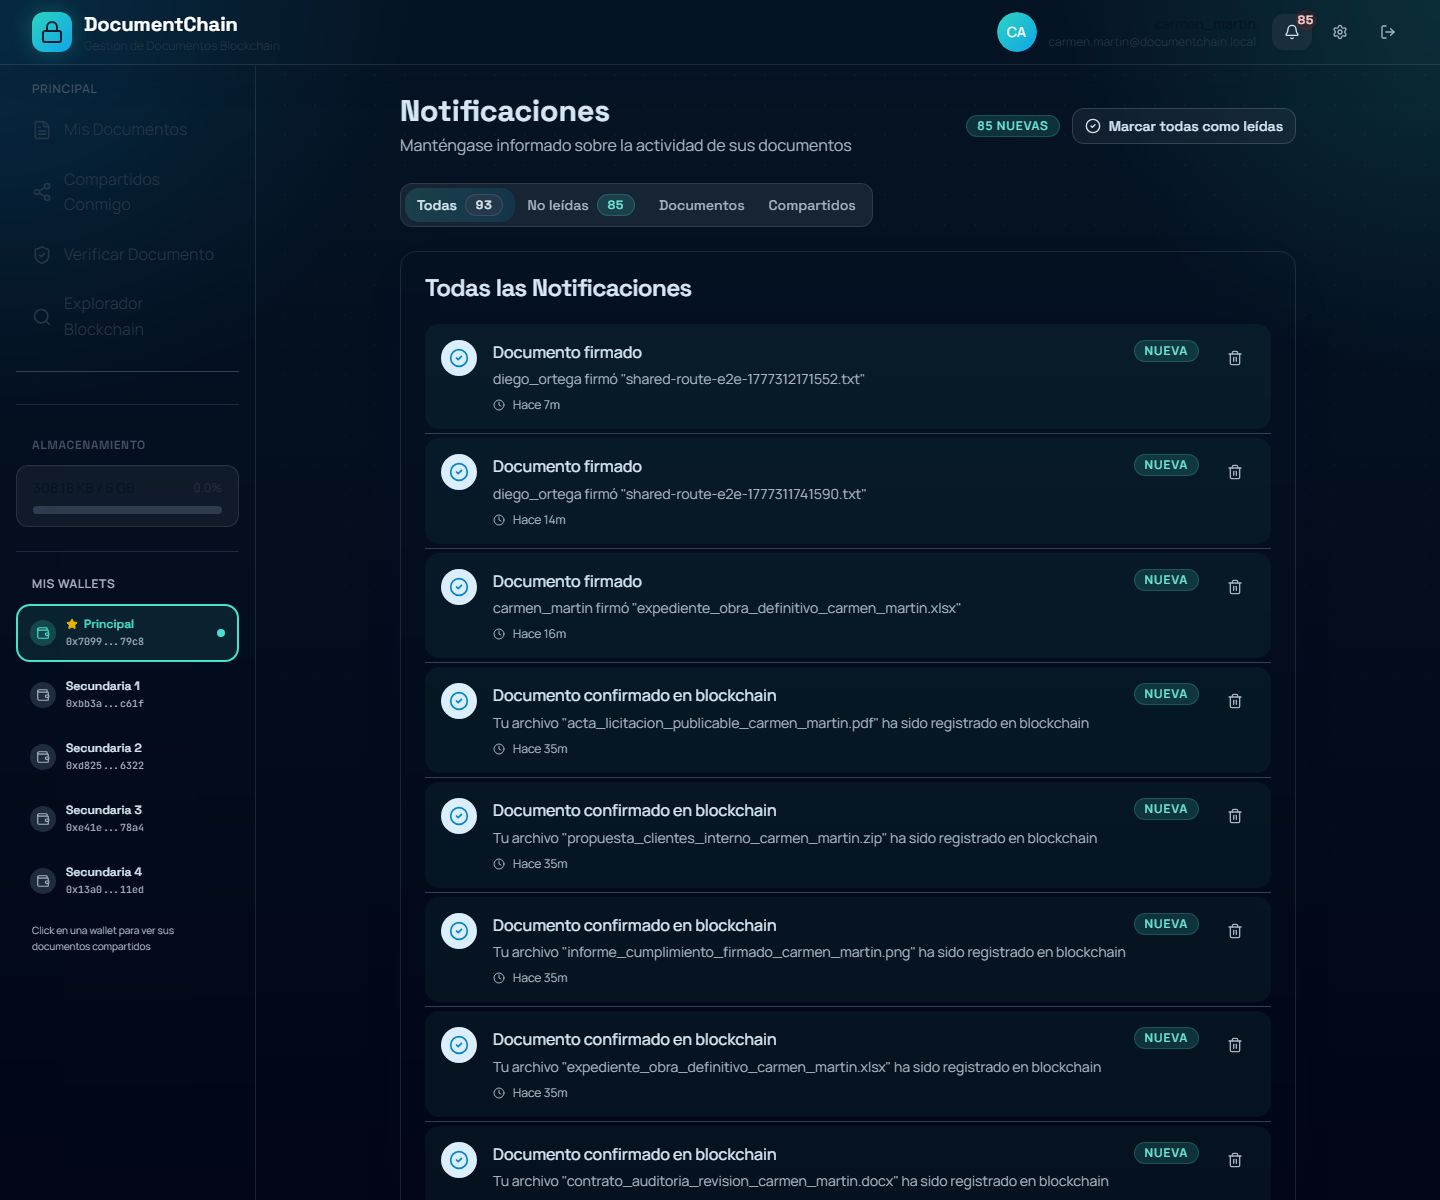
\includegraphics[width=0.90\textwidth]{capturas-ui/notifications-page.png}
    \caption{Centro de notificaciones con eventos pendientes del sistema}
    \label{fig:notif-mem}
\end{figure}

Además de las notificaciones dentro de la aplicación, el sistema envía correos transaccionales para los eventos más críticos: verificación de correo, recuperación de contraseña, notificación de firma y aviso de cambio de contraseña. Las Figuras~\ref{fig:email-verif-mem} y \ref{fig:email-reset-mem} muestran los diseños de esos mensajes.

\begin{figure}[H]
    \centering
    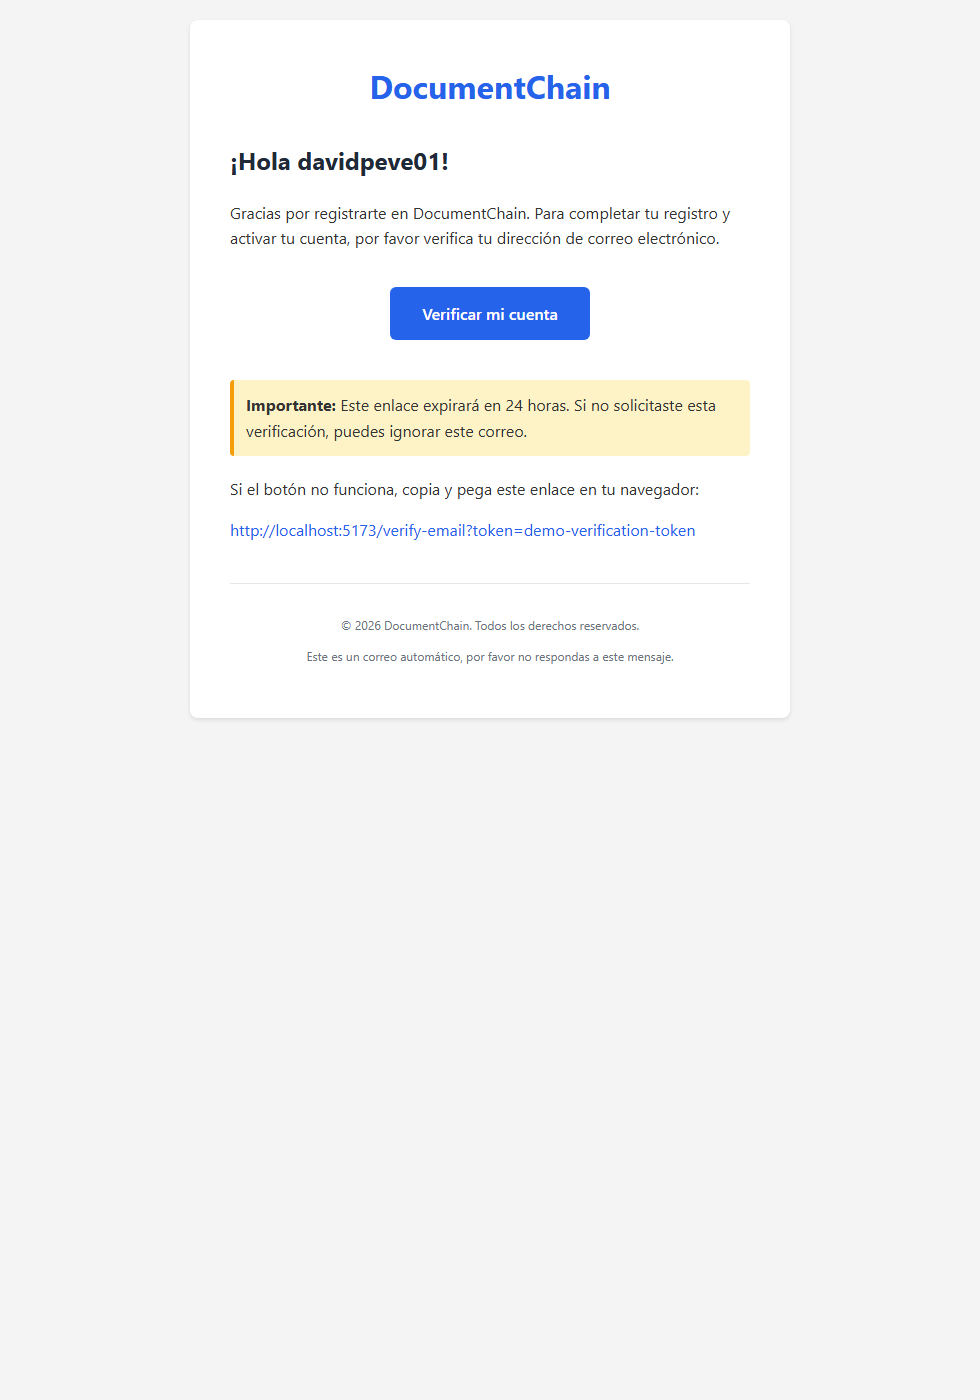
\includegraphics[width=0.75\textwidth]{capturas-ui/email-verification-preview.png}
    \caption{Previsualización del correo de verificación de cuenta enviado al registrarse}
    \label{fig:email-verif-mem}
\end{figure}

\begin{figure}[H]
    \centering
    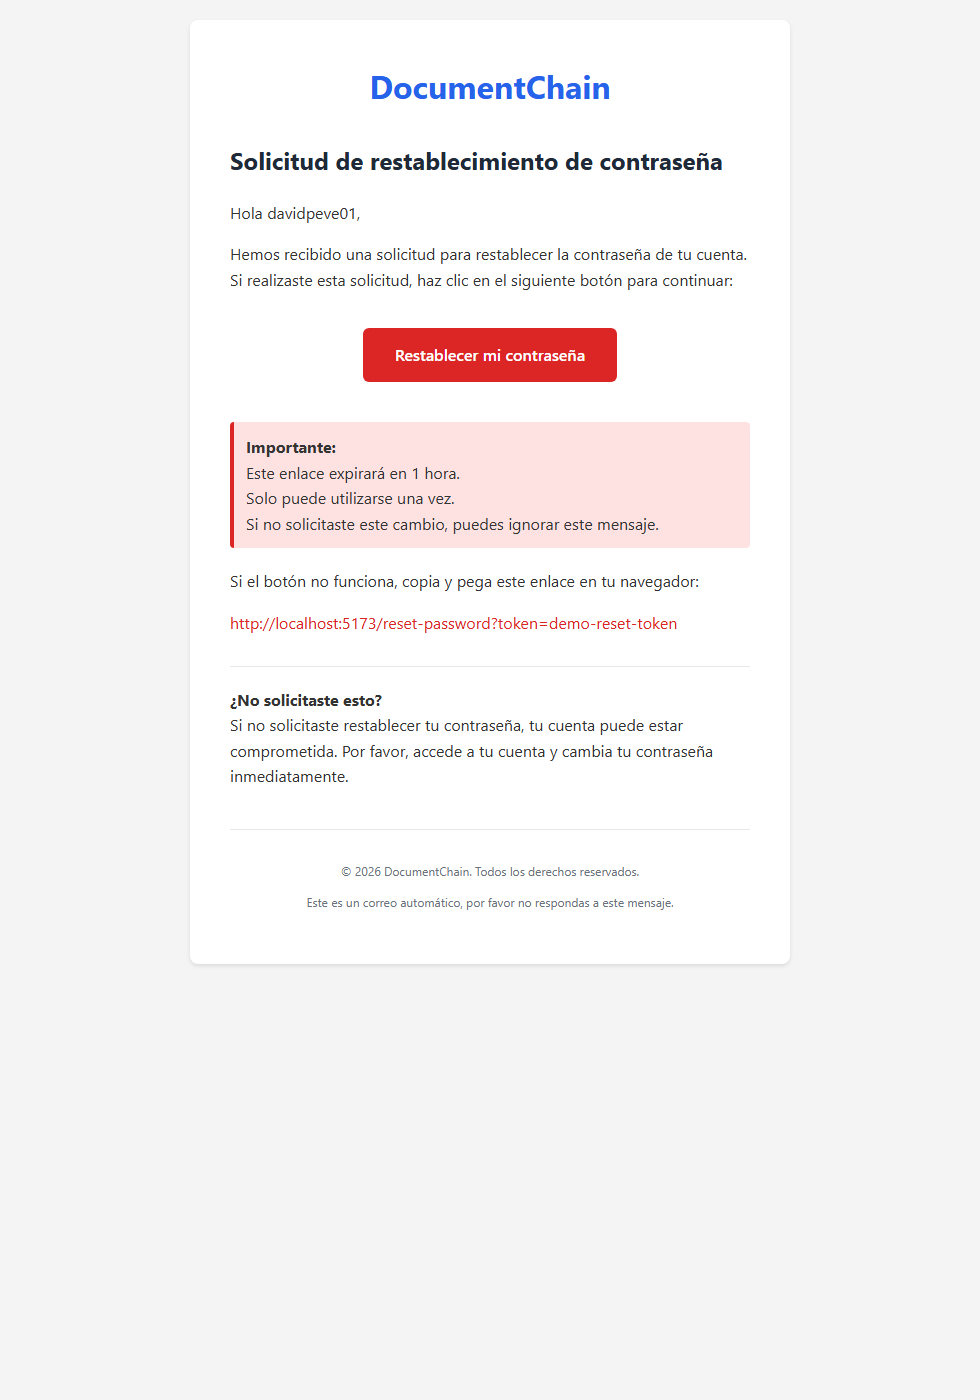
\includegraphics[width=0.75\textwidth]{capturas-ui/email-password-reset-preview.png}
    \caption{Previsualización del correo de recuperación de contraseña}
    \label{fig:email-reset-mem}
\end{figure}

\subsection{Perfil, configuración y preferencias}

El área de perfil permite al usuario gestionar sus datos personales, cambiar contraseña y administrar las wallets vinculadas. La Figura~\ref{fig:profile-mem} muestra esa sección.

\begin{figure}[H]
    \centering
    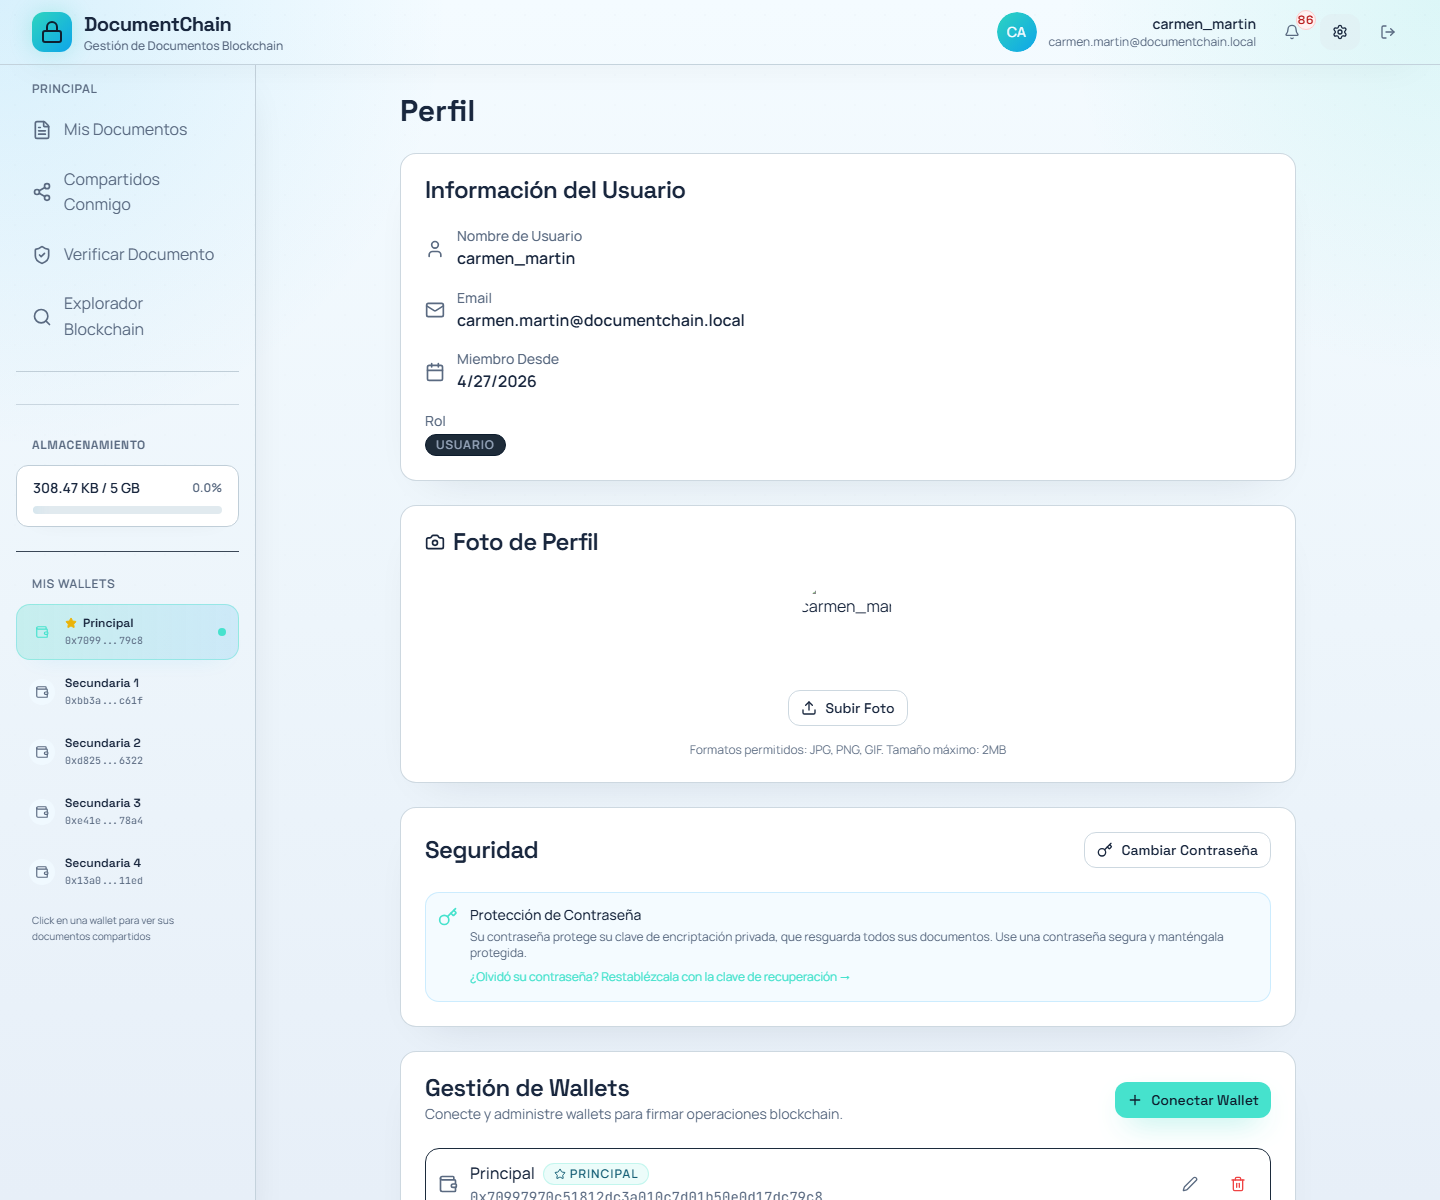
\includegraphics[width=0.90\textwidth]{capturas-ui/profile-page.png}
    \caption{Sección de perfil de usuario con gestión de datos personales y wallets}
    \label{fig:profile-mem}
\end{figure}

La pantalla de configuración permite ajustar las preferencias de notificación, el idioma de la interfaz y las opciones de seguridad adicionales. La Figura~\ref{fig:settings-mem} muestra esa pantalla.

\begin{figure}[H]
    \centering
    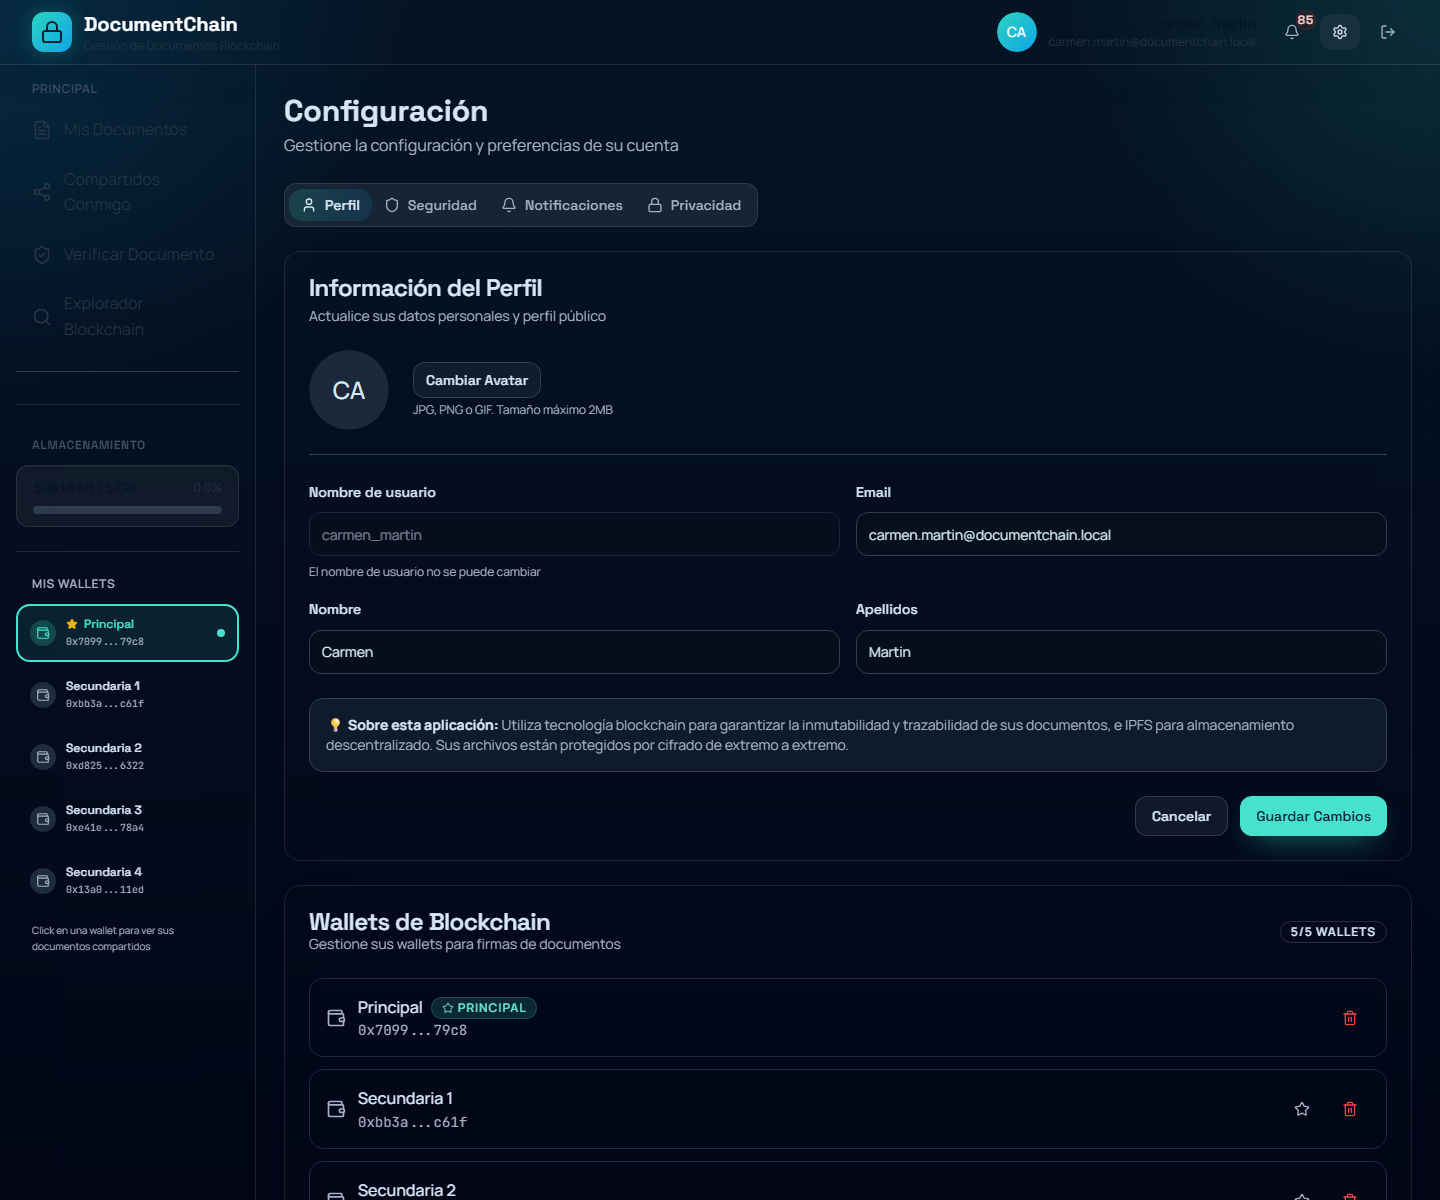
\includegraphics[width=0.90\textwidth]{capturas-ui/settings-page.png}
    \caption{Pantalla de configuración y preferencias de la cuenta}
    \label{fig:settings-mem}
\end{figure}

\subsection{Área pública del sistema}

La solución no se limita a un área autenticada. Se ha diseñado también una capa pública que presenta el sistema, ofrece acceso a registro e inicio de sesión y expone las herramientas de verificación para visitantes sin cuenta. La Figura~\ref{fig:landing-public-memoria} muestra la portada pública.

\begin{figure}[H]
    \centering
    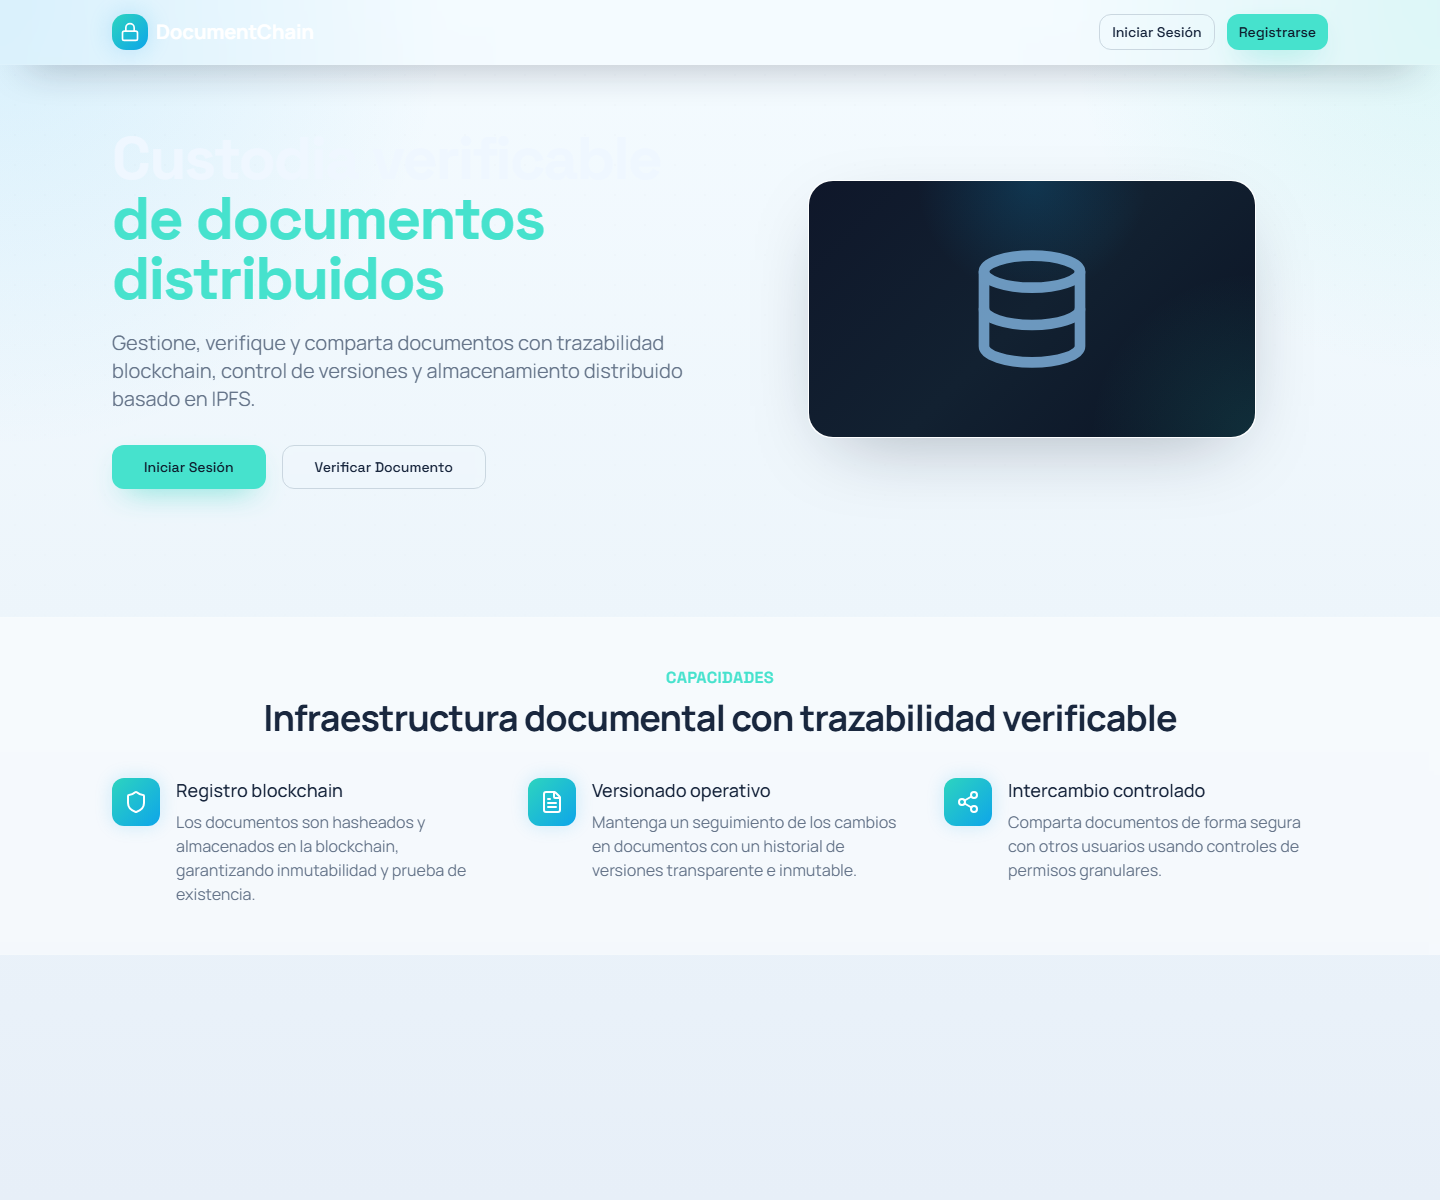
\includegraphics[width=0.93\textwidth]{capturas-ui/landing-public.png}
    \caption{Portada pública del sistema y acceso inicial a sus recorridos principales}
    \label{fig:landing-public-memoria}
\end{figure}

\subsection{Área administrativa}

El sistema incorpora un panel administrativo diferenciado. En él se centralizan la supervisión de usuarios, la revisión de actividad y la consulta de indicadores del sistema. La Figura~\ref{fig:admin-dashboard-memoria} muestra el panel principal.

\begin{figure}[H]
    \centering
    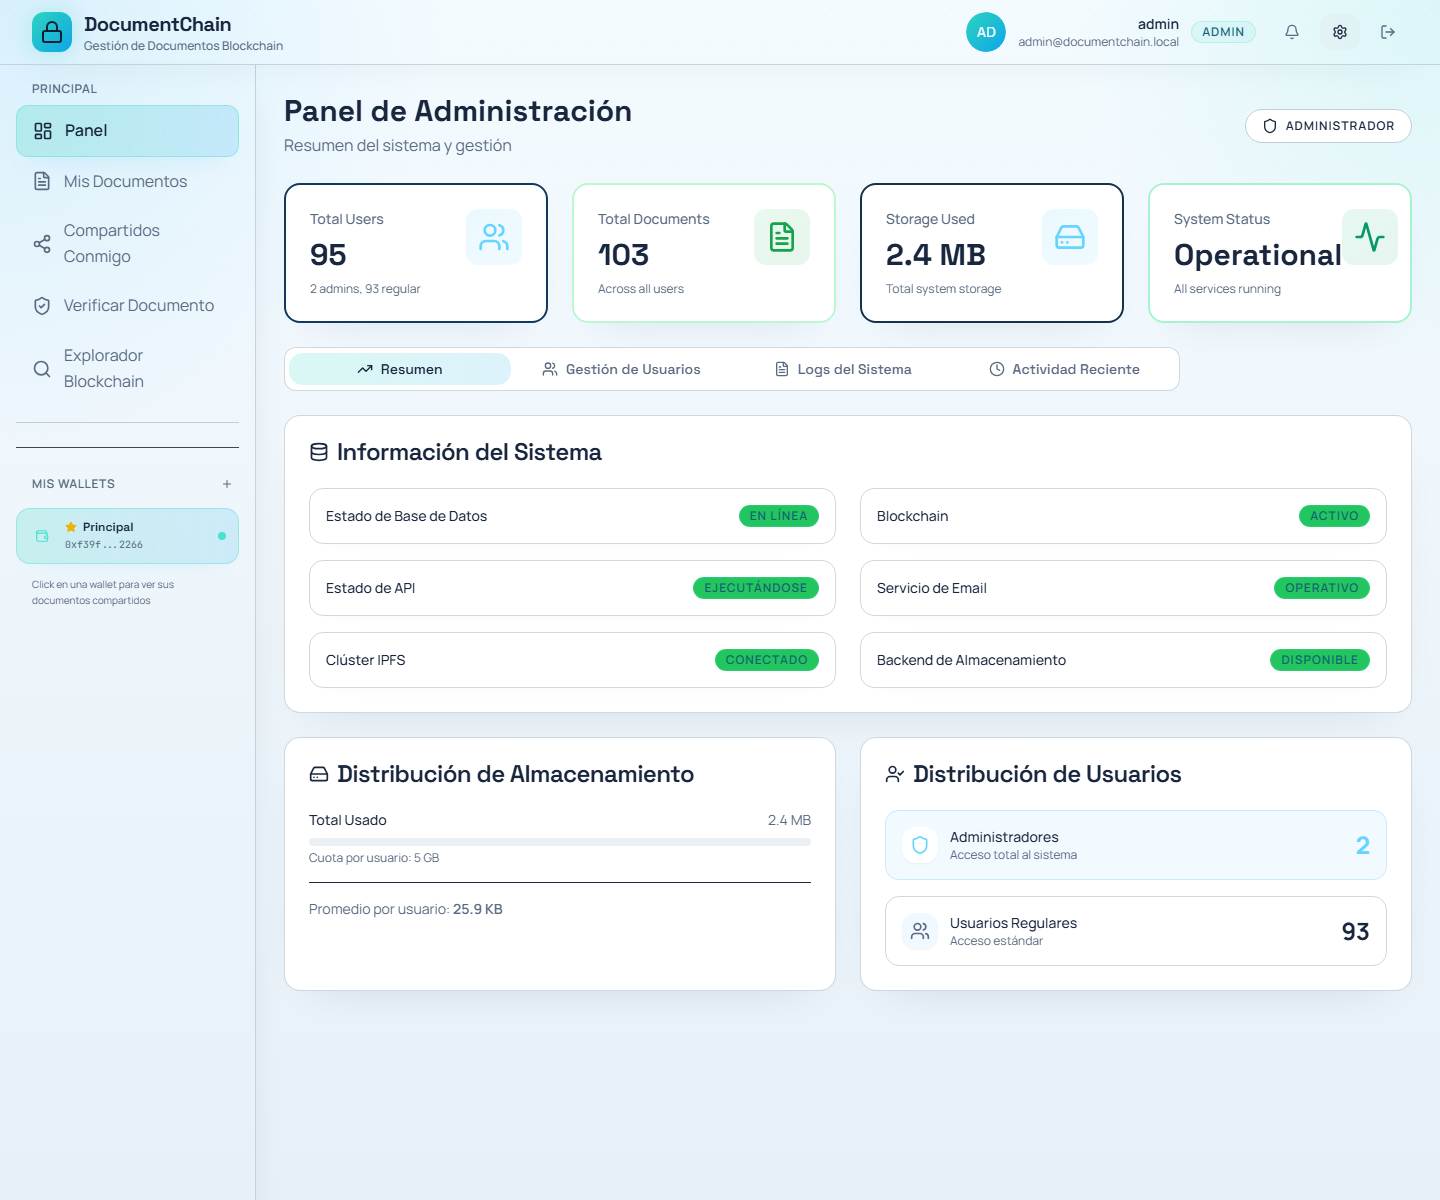
\includegraphics[width=0.92\textwidth]{capturas-ui/admin-dashboard.png}
    \caption{Panel administrativo del sistema con acceso a supervisión y control operativo}
    \label{fig:admin-dashboard-memoria}
\end{figure}

La gestión de usuarios permite al administrador revisar cuentas, consultar su estado y activar o suspender accesos. La Figura~\ref{fig:admin-users-mem} muestra esa sección.

\begin{figure}[H]
    \centering
    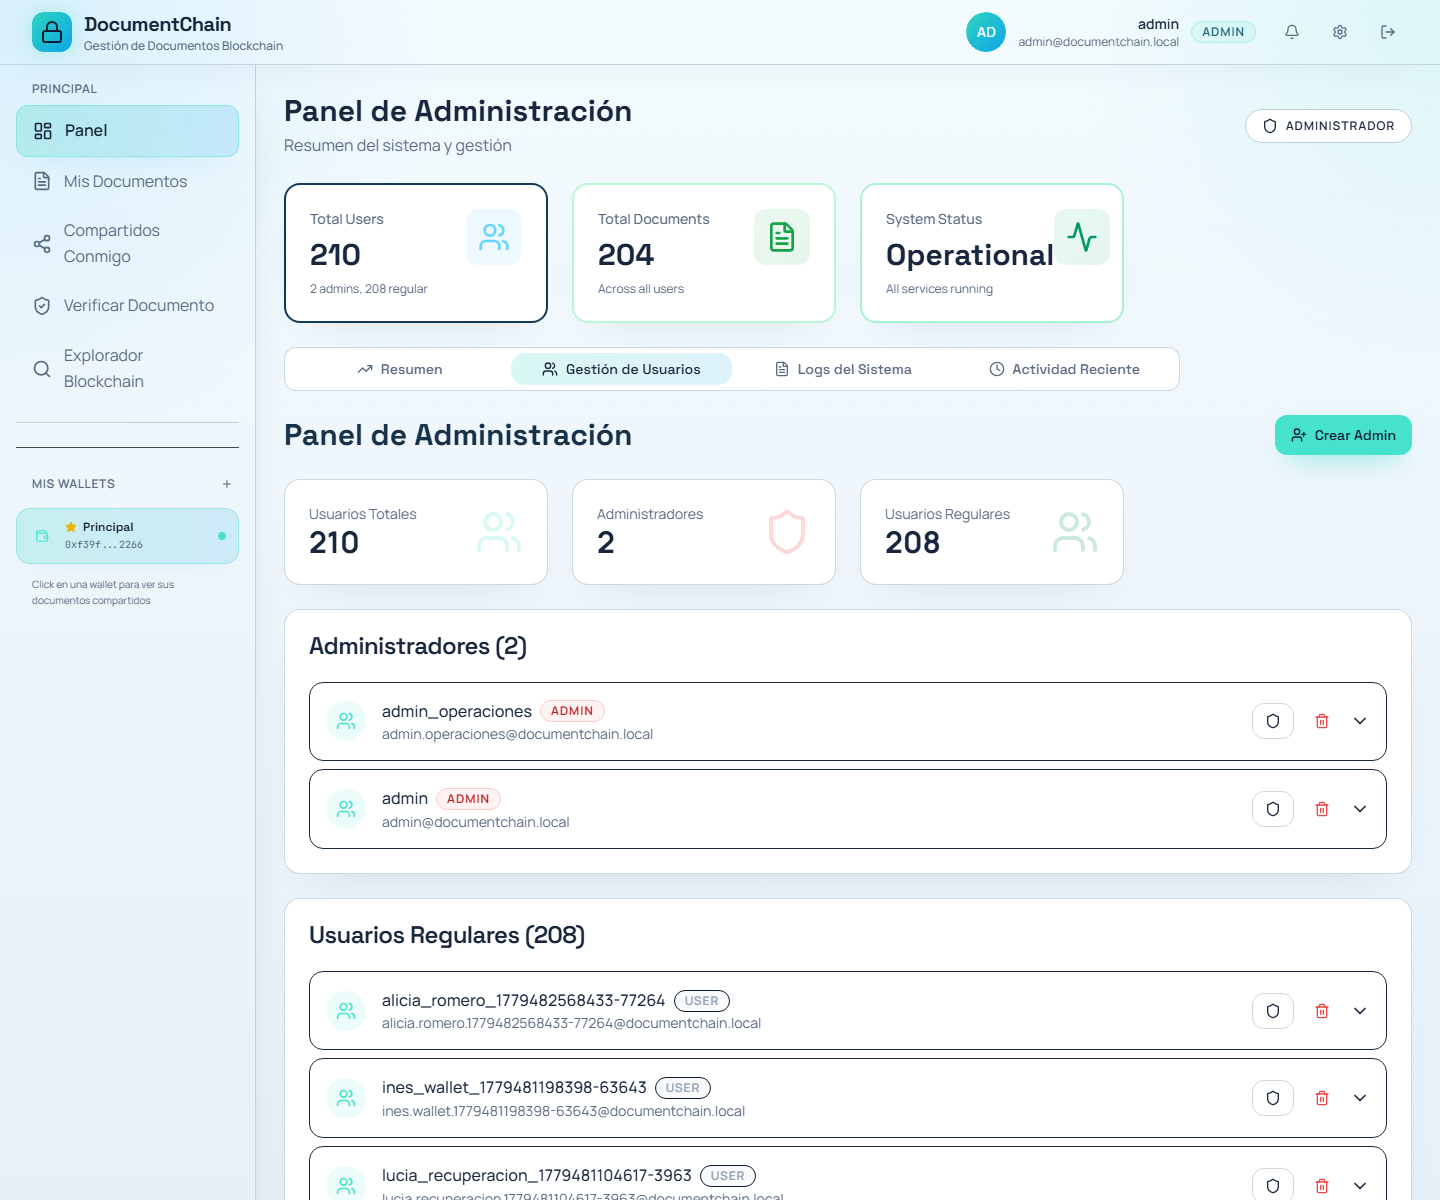
\includegraphics[width=0.92\textwidth]{capturas-ui/admin-users-tab.png}
    \caption{Panel de gestión de usuarios con opciones de supervisión por parte del administrador}
    \label{fig:admin-users-mem}
\end{figure}

El registro de actividad del sistema permite auditar operaciones ejecutadas por todos los usuarios, con filtros por tipo de evento y por usuario. La Figura~\ref{fig:admin-logs-mem} muestra esa vista.

\begin{figure}[H]
    \centering
    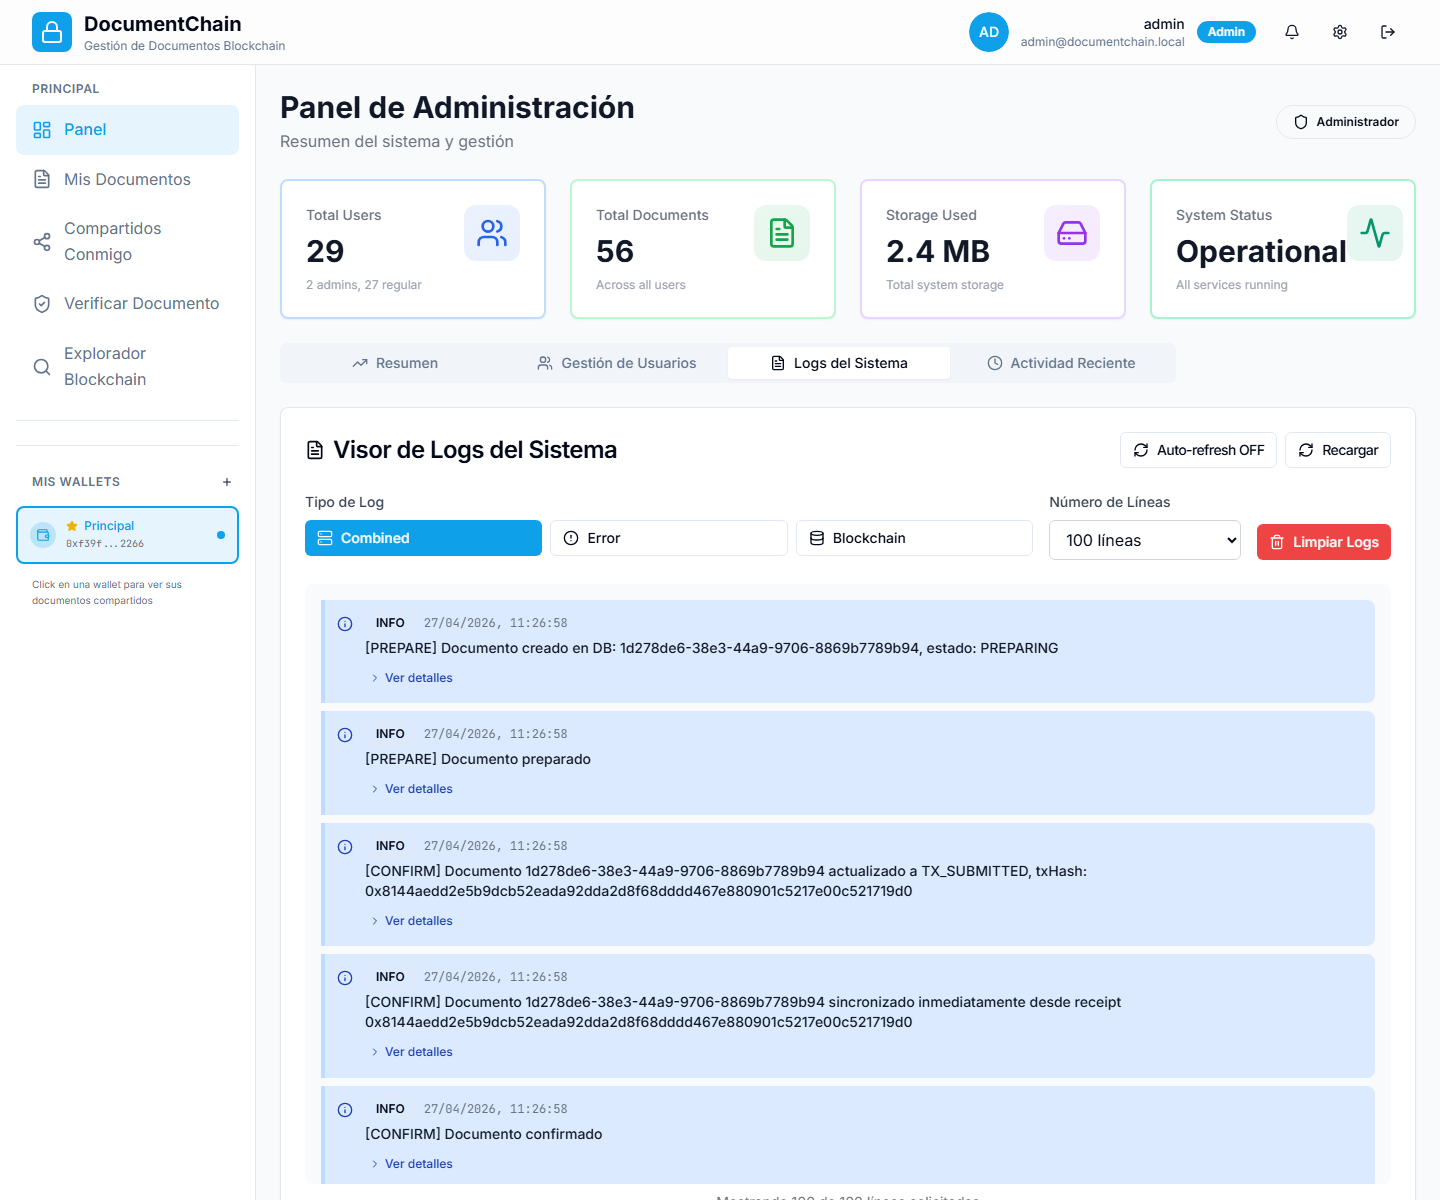
\includegraphics[width=0.92\textwidth]{capturas-ui/admin-logs-tab.png}
    \caption{Registro de actividad del sistema accesible desde el panel administrativo}
    \label{fig:admin-logs-mem}
\end{figure}

\subsection{Exploración técnica y auditoría blockchain}

Una característica especialmente valiosa del proyecto es la existencia de una vista donde la evidencia blockchain se vuelve legible dentro de la propia aplicación. El explorador de actividad on-chain traduce los eventos del contrato a un formato navegable, con referencias a documentos, versiones y direcciones de wallet. La Figura~\ref{fig:blockchain-auditor-memoria} muestra esa vista.

\begin{figure}[H]
    \centering
    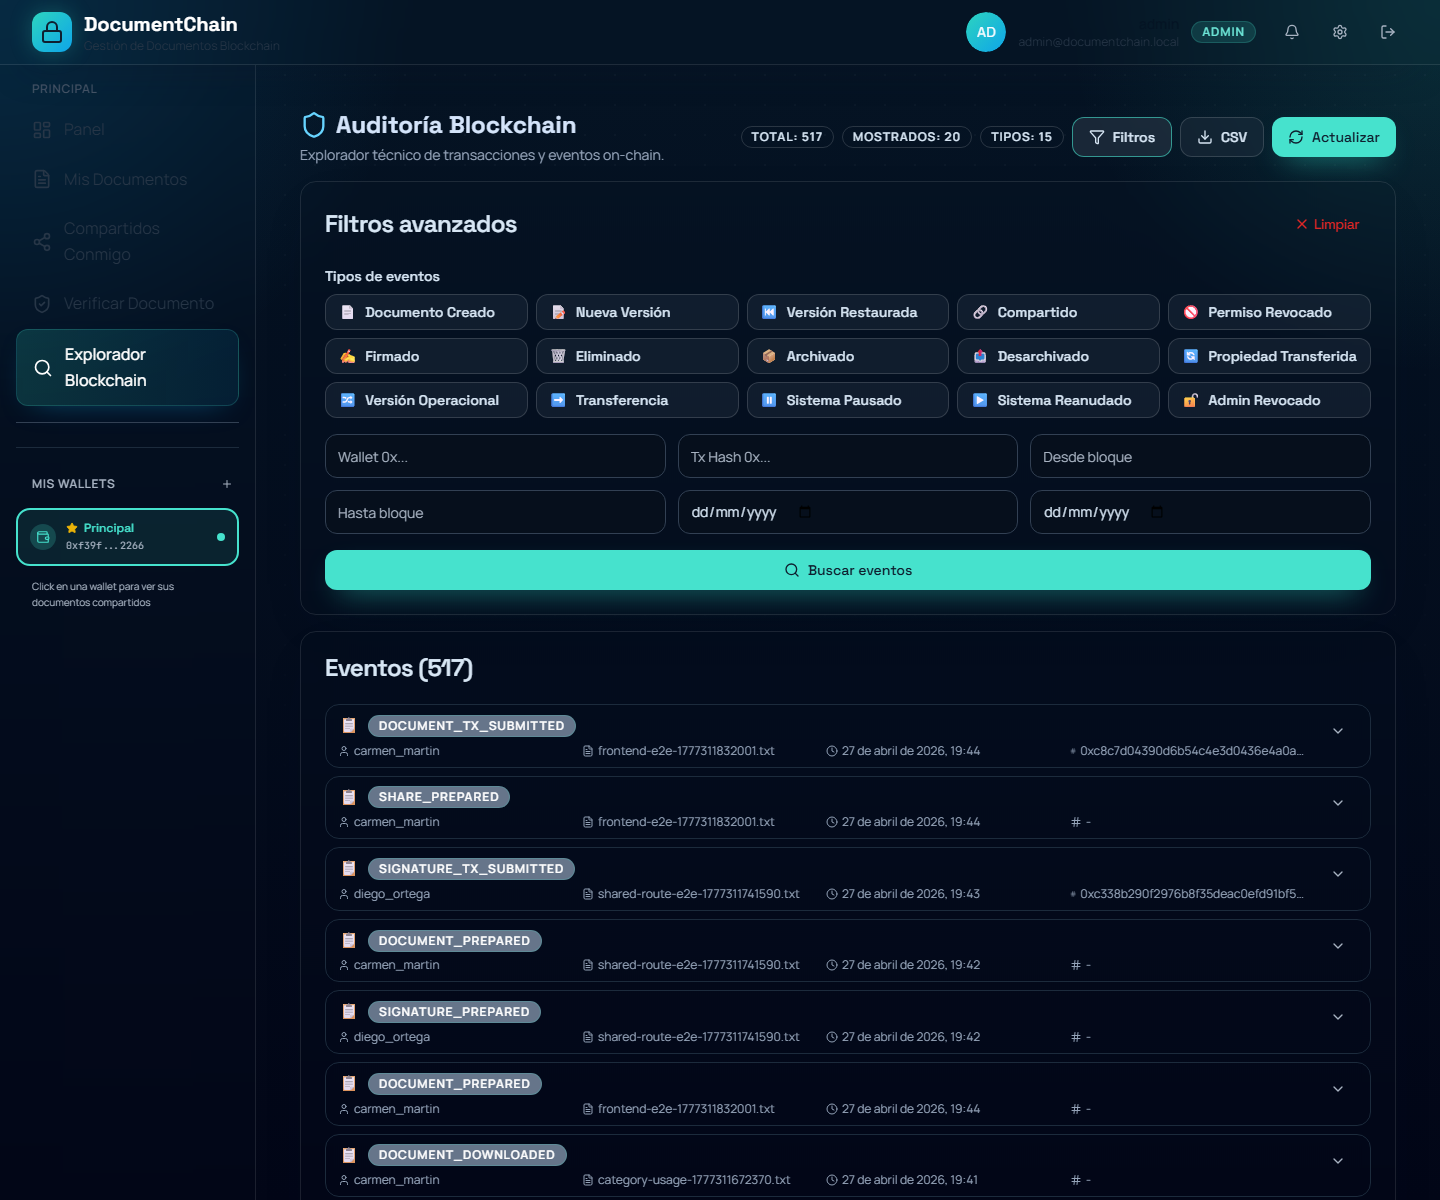
\includegraphics[width=0.92\textwidth]{capturas-ui/blockchain-auditor.png}
    \caption{Vista del explorador técnico de actividad blockchain integrado en la aplicación}
    \label{fig:blockchain-auditor-memoria}
\end{figure}

\subsection{Vídeo demostrativo}

Con objeto de facilitar la comprensión del sistema en contextos donde no sea posible ejecutarlo en vivo, se ha grabado un vídeo demostrativo que recorre los flujos principales de la plataforma. El vídeo muestra el proceso de registro, autenticación con segundo factor opcional, subida de un documento, creación de versión nueva, firma digital con wallet, compartición con otro usuario, acceso desde cuenta compartida, publicación para verificación pública y consulta del explorador de actividad blockchain. La duración total aproximada es de quince minutos y el fichero se entrega junto con la documentación académica del proyecto.

El recorrido reproducido en el vídeo tiene un valor complementario respecto a las capturas estáticas de la interfaz: permite observar las transiciones entre vistas, los tiempos de respuesta reales de las operaciones blockchain, la confirmación visual de la firma en la wallet, y el comportamiento del sistema ante escenarios habituales de uso. Se considera una evidencia de validación adicional que complementa la batería de pruebas automatizadas y los manuales de usuario del Anexo V.

\section{Análisis de riesgos}

\subsection{Matriz de riesgos}

La integración de persistencia relacional, almacenamiento distribuido, firmas con wallet y coordinación blockchain introduce un perfil de riesgo superior al de una aplicación web puramente centralizada. Esa complejidad no se interpreta aquí como defecto inevitable, sino como un conjunto de condicionantes que deben identificarse, priorizarse y mitigarse. La matriz de la Tabla~\ref{tab:matriz-riesgos-memoria} resume los riesgos con mayor capacidad de afectar a la entrega académica o a la consistencia funcional del sistema.

\begin{table}[H]
    \centering
    \small
    \begin{tabular}{|p{0.9cm}|p{5.2cm}|p{1.9cm}|p{1.9cm}|p{1.4cm}|p{1.9cm}|}
    \hline
    \textbf{ID} & \textbf{Riesgo identificado} & \textbf{Prob.} & \textbf{Sever.} & \textbf{Valor} & \textbf{Nivel} \\
    \hline
    R1 & Desalineación entre estado \textit{on-chain} y estado operativo en PostgreSQL & 3 & 4 & 12 & Medio-alto \\
    \hline
    R2 & Dependencia del nodo IPFS autoalojado o de la persistencia efectiva del CID & 2 & 4 & 8 & Medio \\
    \hline
    R3 & Fricción de uso derivada de wallet y firma de operaciones críticas & 3 & 3 & 9 & Medio \\
    \hline
    R4 & Incidencias de salida SMTP real por reputación o configuración del relay & 3 & 3 & 9 & Medio \\
    \hline
    R5 & Exposición accidental de un documento al activar visibilidad pública & 2 & 5 & 10 & Medio \\
    \hline
    R6 & Complejidad de despliegue y demostración por coexistencia de varios servicios & 3 & 4 & 12 & Medio-alto \\
    \hline
    R7 & Pérdida o mala gestión del material de acceso del usuario & 2 & 5 & 10 & Medio \\
    \hline
    \end{tabular}
    \caption{Matriz resumida de riesgos del proyecto DocumentChain}
    \label{tab:matriz-riesgos-memoria}
\end{table}

\subsection{Análisis DAFO}

Además de la matriz clásica, resulta útil observar el proyecto desde una perspectiva DAFO, porque permite distinguir entre limitaciones internas y condicionantes externos. Esta lectura es pertinente en una memoria académica extensa, ya que no todo riesgo proviene de un fallo técnico; parte del contexto depende de adopción, infraestructura disponible o madurez de ciertas integraciones.

\begin{table}[H]
    \centering
    \small
    \begin{tabular}{|p{3cm}|p{10.5cm}|}
    \hline
    \textbf{Dimensión} & \textbf{Síntesis} \\
    \hline
    Fortalezas & Arquitectura híbrida bien delimitada, trazabilidad verificable, separación entre identidad de cuenta y firma, documentación abundante y despliegue reproducible. \\
    \hline
    Debilidades & Complejidad superior a la de una aplicación documental convencional, dependencia de varias capas para una sola operación y necesidad de explicar bien al usuario el alcance de la wallet y de la publicación pública. \\
    \hline
    Oportunidades & Aplicación del modelo a dominios donde la trazabilidad importe, extensión a redes distintas de desarrollo, incorporación de observabilidad avanzada y reutilización académica de la arquitectura. \\
    \hline
    Amenazas & Cambios en políticas de proveedores, rechazo de correo por reputación externa, fricción de adopción por parte de usuarios no familiarizados con wallets y costes crecientes si se migrara a una red pública permanente. \\
    \hline
    \end{tabular}
    \caption{Síntesis DAFO del proyecto desde la perspectiva técnica y operativa}
    \label{tab:dafo-memoria}
\end{table}

\subsection{Registro de riesgos prioritarios y respuesta adoptada}

El tratamiento práctico del riesgo en el proyecto se ha orientado a decisiones de diseño concretas. El patrón \textit{prepare/confirm} se adopta para desacoplar preparación operativa y consolidación on-chain. La persistencia del nodo Kubo autoalojado sobre volúmenes propios reduce dependencia rígida de una infraestructura externa y mantiene bajo control directo la conservación de los CIDs activos. La salida SMTP a través de Postfix más relay autenticado evita presentar como estable una entrega directa a Internet que no depende solo de la aplicación. Y la interfaz diferencia visibilidad pública y privada para reducir errores de publicación.

\begin{table}[H]
    \centering
    \small
    \begin{tabular}{|p{3.1cm}|p{3.8cm}|p{6.2cm}|}
    \hline
    \textbf{Riesgo} & \textbf{Disparador representativo} & \textbf{Respuesta adoptada} \\
    \hline
    Inconsistencia entre capas & Transacción enviada pero no confirmada o no sincronizada & Estados intermedios, reconciliación posterior y separación \textit{prepare/confirm}. \\
    \hline
    Dependencia de infraestructura IPFS & Pérdida de pinning o indisponibilidad del nodo autoalojado & Persistencia en volúmenes, abstracción del acceso IPFS y registro del CID en el ciclo de versión. \\
    \hline
    Fricción de firma & Usuario sin wallet activa o con baja comprensión del flujo & Wallet reservada para operaciones críticas y autenticación ordinaria independiente. \\
    \hline
    Entrega de correo no fiable & Rechazo del destinatario o ausencia de reputación & Postfix interno desacoplado del backend y uso de relay autenticado. \\
    \hline
    Publicación errónea & Cambio accidental de visibilidad del documento & Advertencia visible, diferenciación de estados y acceso público solo mediante acción expresa. \\
    \hline
    \end{tabular}
    \caption{Registro resumido de riesgos prioritarios y respuestas de diseño}
    \label{tab:registro-riesgos-memoria}
\end{table}

\section{Organización y gestión del proyecto}

La gestión del proyecto ha combinado trabajo técnico sobre código, contratos, esquemas y configuración con seguimiento documental de decisiones, diseño, pruebas y operación. En este apartado se exponen los aspectos técnicos más relevantes de los componentes principales del sistema, se describe el desarrollo llevado a cabo y se detalla la planificación seguida.

\subsection{Aspectos relevantes del frontend}

La interfaz se construye como SPA en React, usando Vite como herramienta de construcción y TypeScript como lenguaje de implementación. La gestión de rutas se resuelve con React Router, con rutas protegidas que verifican el estado de sesión antes de renderizar. El estado global se distribuye en tres contextos principales: autenticación (usuario, token, sesión activa), wallet (proveedor Ethers, signer, dirección activa y red) y notificaciones (estado de alertas en tiempo real). Esa separación es arquitectónicamente importante porque los ciclos de vida de la sesión de cuenta y de la conexión con la wallet son distintos: la sesión puede existir sin wallet activa, y la wallet puede cambiar sin que expire la sesión.

Las operaciones documentales se exponen mediante hooks personalizados que abstraen las llamadas a la API y gestionan de forma uniforme los estados de carga y error. La integración blockchain utiliza Ethers.js para conectar con el proveedor de MetaMask, gestionar el cambio de red cuando es necesario y exponer el signer para las operaciones que requieren firma. La decisión arquitectónica más relevante es que la wallet nunca se exige para navegar por la aplicación ni para consultar documentos; solo se activa cuando el usuario inicia una operación que debe quedar registrada on-chain. Eso mantiene la experiencia cotidiana razonablemente fluida sin trivializar el valor probatorio de la firma.

\begin{figure}[H]
    \centering
    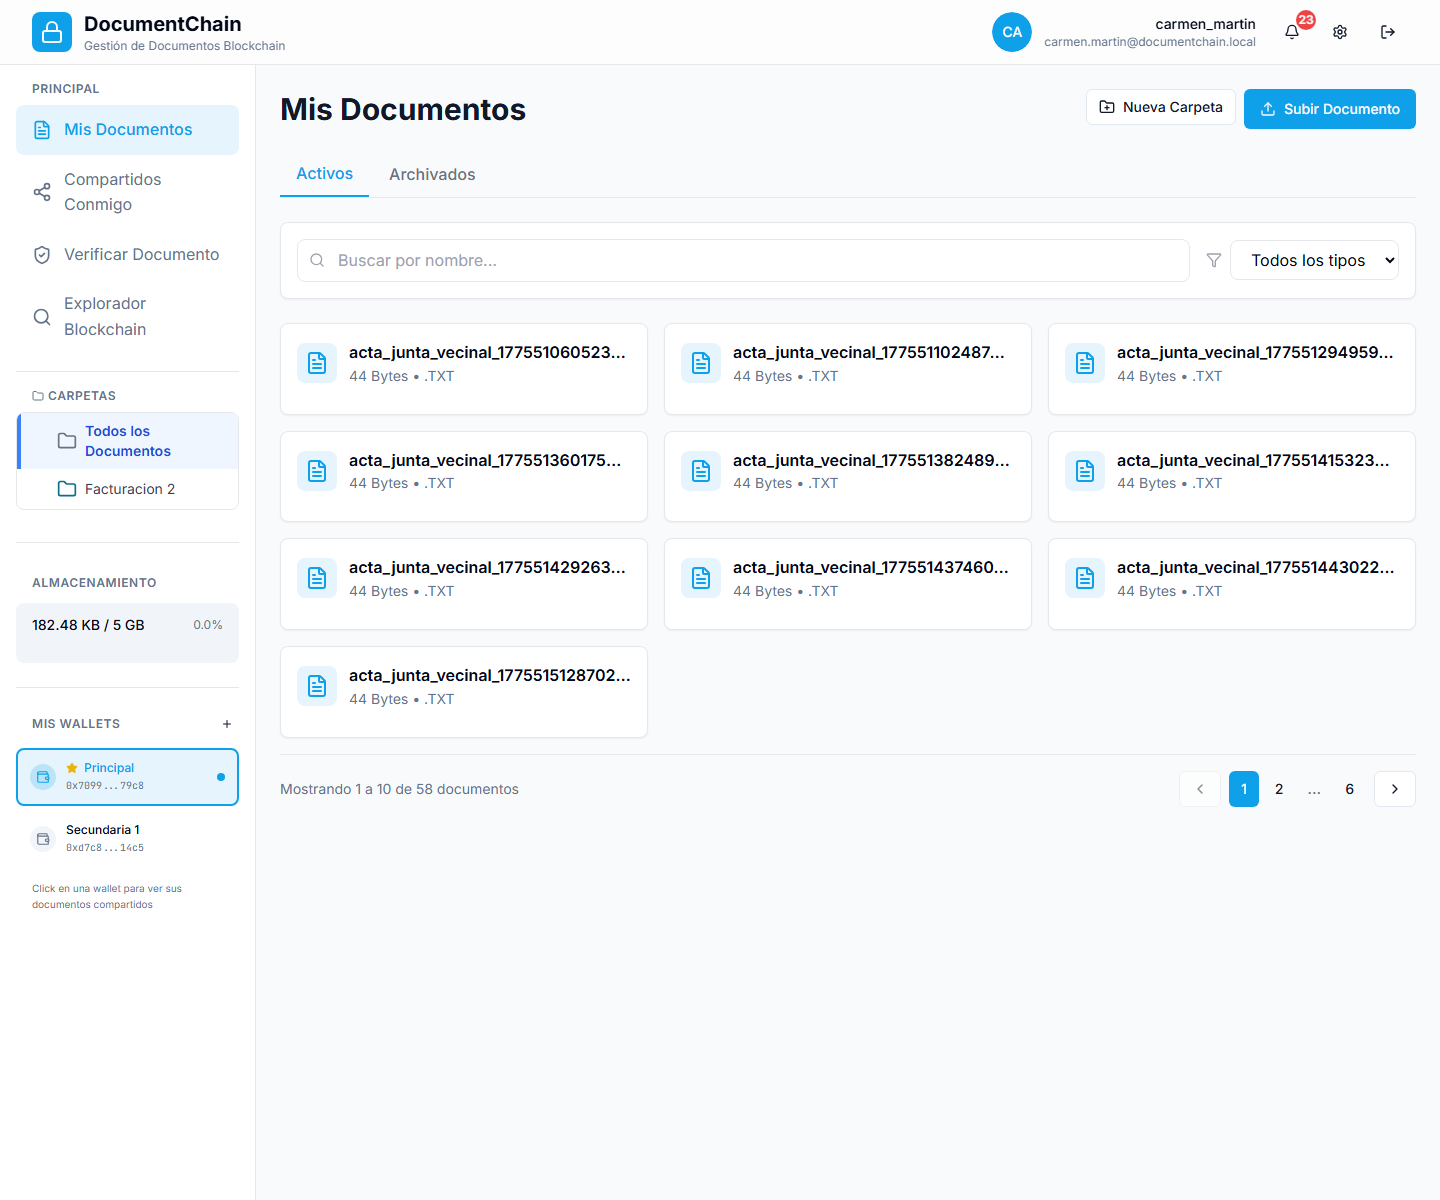
\includegraphics[width=0.92\textwidth]{capturas-ui/documents-page.png}
    \caption{Vista principal del panel de documentos con las acciones disponibles para el usuario}
    \label{fig:documents-page-org}
\end{figure}

\subsection{Aspectos relevantes del backend}

El backend sigue una arquitectura en capas donde los controladores gestionan la validación de la petición HTTP y la construcción de la respuesta, los servicios contienen la lógica de negocio y coordinan las integraciones, y Prisma gestiona el acceso a los datos relacionales. Cada dominio de la aplicación (autenticación, documentos, versiones, compartición, firmas, administración) tiene su propio par controlador--servicio, lo que facilita el mantenimiento y el aislamiento de cambios.

Los servicios transversales se instancian como singletons inyectados donde son necesarios. El servicio criptográfico encapsula el cifrado AES-256-GCM, el descifrado autenticado y la protección asimétrica de claves simétricas. El servicio IPFS concentra el acceso al nodo Kubo autoalojado y mantiene el backend desacoplado de los detalles del protocolo HTTP subyacente. El servicio blockchain construye transacciones con Ethers.js, las monitoriza mediante listeners de eventos y actualiza el estado operativo una vez confirmadas. El servicio de correo genera plantillas HTML para notificaciones transaccionales y encola la entrega a través de Postfix. Esta organización hace que los controladores permanezcan relativamente delgados y que la lógica de negocio compleja pueda probarse de forma independiente del transporte HTTP.

\begin{figure}[H]
    \centering
    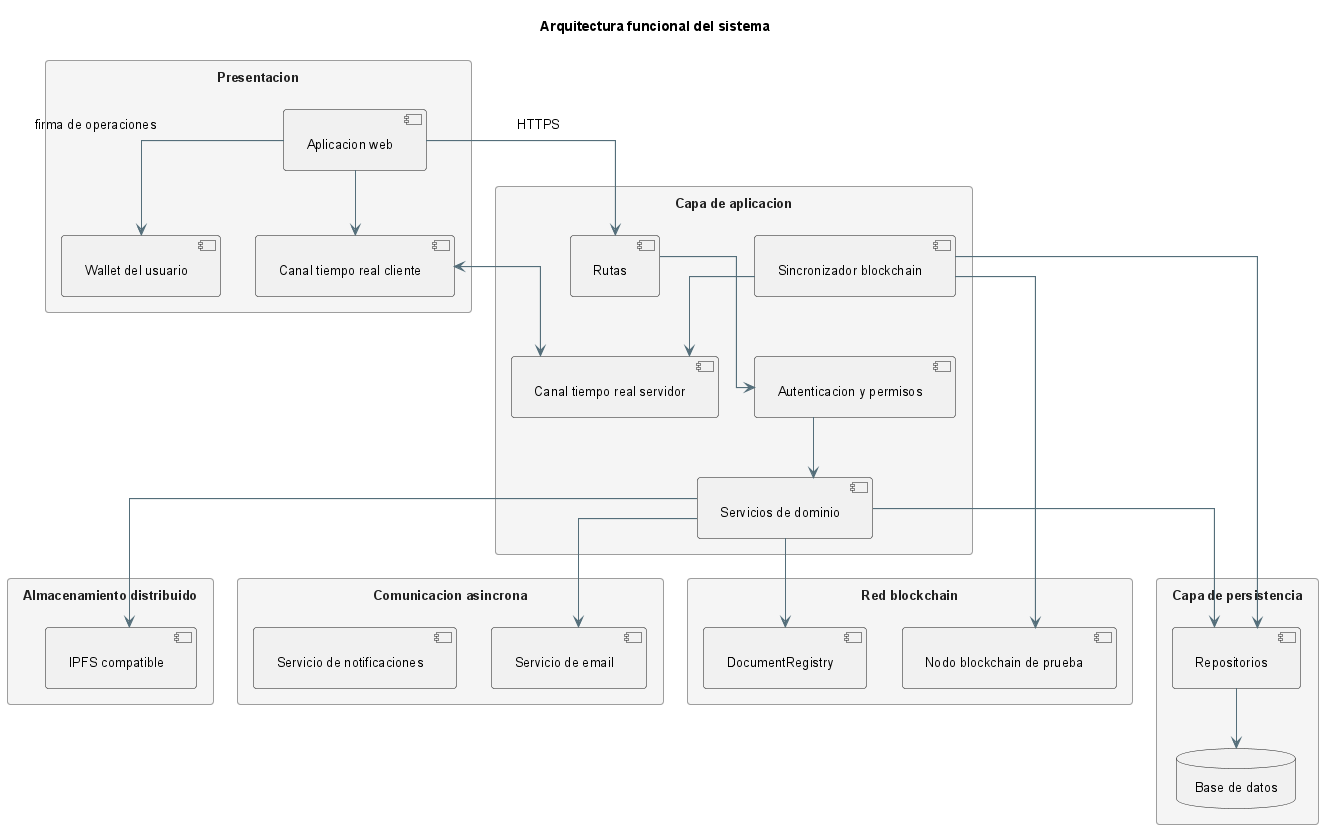
\includegraphics[width=0.92\textwidth]{diagramas/arquitectura.png}
    \caption{Diagrama de arquitectura por capas del sistema y sus responsabilidades}
    \label{fig:arquitectura-org}
\end{figure}

\subsection{Descripción del desarrollo}

\subsubsection{Arquitectura por capas y componentes}

La arquitectura de DocumentChain se apoya en una separación por capas que reduce acoplamiento entre interfaz, lógica de negocio y persistencia. El frontend opera como SPA y concentra rutas, páginas, contextos y componentes reutilizables. El backend expone la API REST, organiza su lógica en controladores y servicios y delega el acceso a datos en Prisma. Las integraciones con blockchain, correo y almacenamiento se modelan como servicios independientes, lo que facilita su evolución y sus pruebas.

\begin{figure}[H]
    \centering
    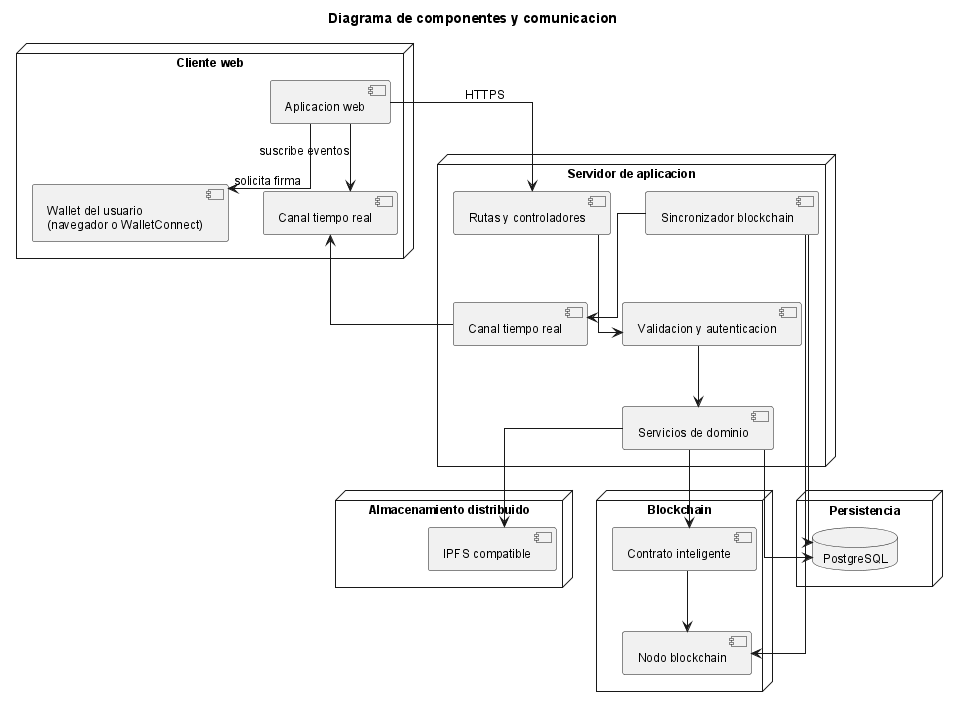
\includegraphics[width=0.92\textwidth]{diagramas/components.png}
    \caption{Diagrama de componentes principales del sistema}
    \label{fig:components}
\end{figure}

\subsubsection{Persistencia y almacenamiento distribuido}

Una de las decisiones centrales del proyecto consiste en no jerarquizar artificialmente PostgreSQL, IPFS y blockchain como si una de las tres capas fuese subordinada a las otras. Cada una mantiene una responsabilidad propia y el sistema completo depende de la coordinación entre ellas. PostgreSQL conserva el estado mutable y consultable; IPFS mantiene el contenido; blockchain conserva la evidencia mínima que interesa poder contrastar de forma independiente.

\begin{figure}[H]
    \centering
    
\includegraphics[width=0.96\textwidth]{diagramas/er-combined.png}
    \caption{Modelo integrado de persistencia entre PostgreSQL, IPFS y blockchain}
    \label{fig:er-combined-memoria}
\end{figure}

\begin{table}[H]
    \centering
    \small
    \begin{tabular}{|p{2.7cm}|p{4.9cm}|p{5.9cm}|}
    \hline
    \textbf{Capa} & \textbf{Qué conserva} & \textbf{Motivo principal} \\
    \hline
    PostgreSQL & Usuarios, sesiones, preferencias de notificación, carpetas, notificaciones y proyecciones de consulta & Permite modelado rico, búsquedas, filtros y actualización frecuente con bajo coste operativo. \\
    \hline
    IPFS & Ficheros documentales y versiones, cifrados o en claro según su visibilidad & Aporta direccionamiento por contenido y desacopla el binario del backend principal. \\
    \hline
    Blockchain & Identificador documental, CID, roles efectivos, firmas, archivado, borrado lógico y cambios de titularidad & Conserva la parte verificable de mayor interés para auditoría y no repudio. \\
    \hline
    \end{tabular}
    \caption{Reparto de responsabilidades entre las capas de persistencia}
    \label{tab:capas-persistencia-memoria}
\end{table}

\subsubsection{Contrato inteligente y modelo on-chain}

El contrato activo del proyecto es \texttt{DocumentRegistry}, un contrato unificado que integra registro documental, versionado, firmas, permisos documentales, suspensión de usuarios y pausa de emergencia. Esta consolidación reduce el número de llamadas necesarias desde el frontend y simplifica la correlación entre operación de negocio y evento emitido.

Las estructuras \texttt{Document}, \texttt{Version} y \texttt{Signature}, junto con los \textit{mappings} de permisos y colecciones enumerables, permiten representar la parte mínima del dominio que debe conservarse como fuente de verdad externa. El contrato no intenta replicar la totalidad del modelo relacional. Mantiene únicamente aquello cuyo valor reside en que no pueda alterarse silenciosamente.

\begin{table}[H]
    \centering
    \small
    \begin{tabular}{|p{3cm}|p{4.5cm}|p{6cm}|}
    \hline
    \textbf{Elemento} & \textbf{Información principal} & \textbf{Papel dentro del sistema} \\
    \hline
    \texttt{Document} & Propietario, versión actual, versión más reciente, estado de archivado o borrado & Expresa el estado documental mínimo verificable. \\
    \hline
    \texttt{Version} & Número de versión, CID, autor, versión operativa y referencia restaurada & Vincula cada hito documental con un contenido concreto y con su posición en el histórico. \\
    \hline
    \texttt{Signature} & Firmante, mensaje, comentario y marca temporal & Conserva evidencia de aceptación o conformidad asociada a una wallet concreta. \\
    \hline
    \texttt{DocumentRole} & NONE, VIEWER, EDITOR, OWNER & Determina el acceso efectivo sobre cada documento. \\
    \hline
    \end{tabular}
    \caption{Elementos on-chain más relevantes del contrato \texttt{DocumentRegistry}}
    \label{tab:contract-model}
\end{table}

\subsubsection{Patrón \textit{prepare/confirm}}

La interacción entre backend y blockchain no se resuelve en una única operación atómica desde servidor porque la firma de la transacción debe realizarla la wallet del usuario en cliente. Para coordinar ese requisito se utiliza un patrón \textit{prepare/confirm}. En la fase de preparación, el backend valida la operación, cifra cuando corresponde, sube el contenido a IPFS y deja el estado en \texttt{PREPARING}. Después el frontend solicita la firma y, una vez emitida la transacción, se ejecuta la confirmación que actualiza el estado hacia \texttt{TX\_SUBMITTED} y finalmente hacia \texttt{SYNCED}.

\begin{figure}[H]
    \centering
    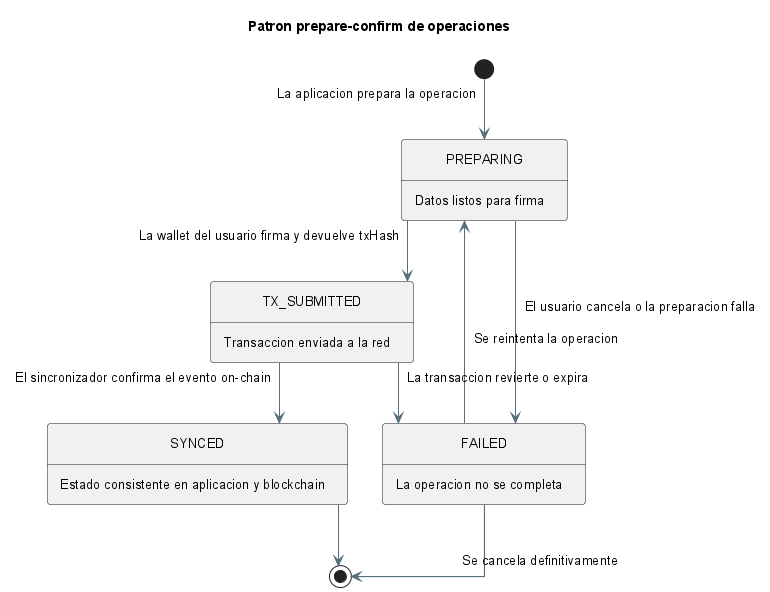
\includegraphics[width=0.92\textwidth]{diagramas/prepare-confirm.png}
    \caption{Patrón \textit{prepare/confirm} aplicado a operaciones críticas}
    \label{fig:prepare-confirm}
\end{figure}

\subsubsection{Diagramas de secuencia representativos}

Los diagramas de secuencia siguientes detallan los intercambios de mensajes entre actores y componentes en los flujos más relevantes del sistema. Su inclusión permite asociar la arquitectura descrita con el comportamiento observable durante la validación.

La Figura~\ref{fig:seq-login-mem} muestra el flujo de autenticación, que incluye la verificación de credenciales, la generación de token y la comprobación opcional del segundo factor.

\begin{figure}[H]
    \centering
    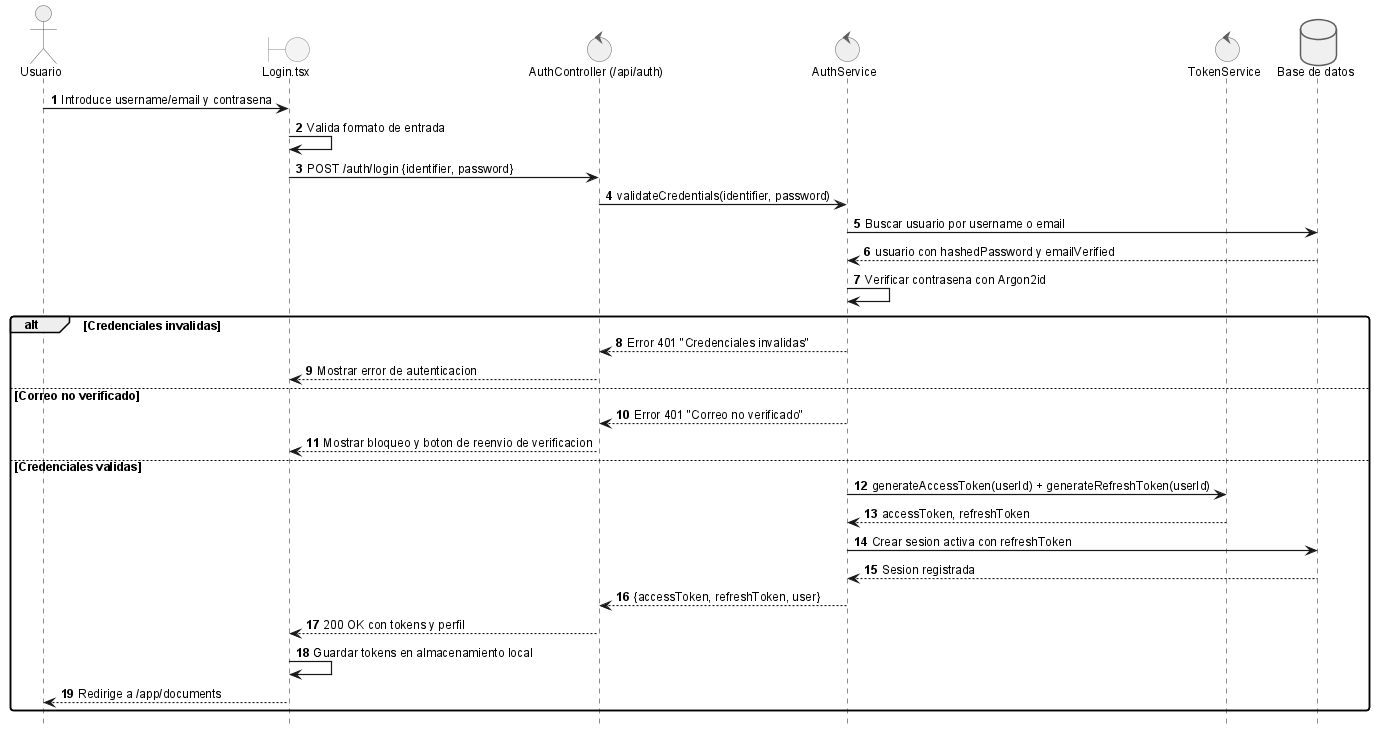
\includegraphics[width=0.92\textwidth]{diagramas/seq-login.png}
    \caption{Diagrama de secuencia del flujo de inicio de sesión con 2FA opcional}
    \label{fig:seq-login-mem}
\end{figure}

La Figura~\ref{fig:seq-register-mem} detalla el proceso de registro de nuevo usuario, que incluye la creación de cuenta, el envío del correo de verificación y la confirmación posterior.

\begin{figure}[H]
    \centering
    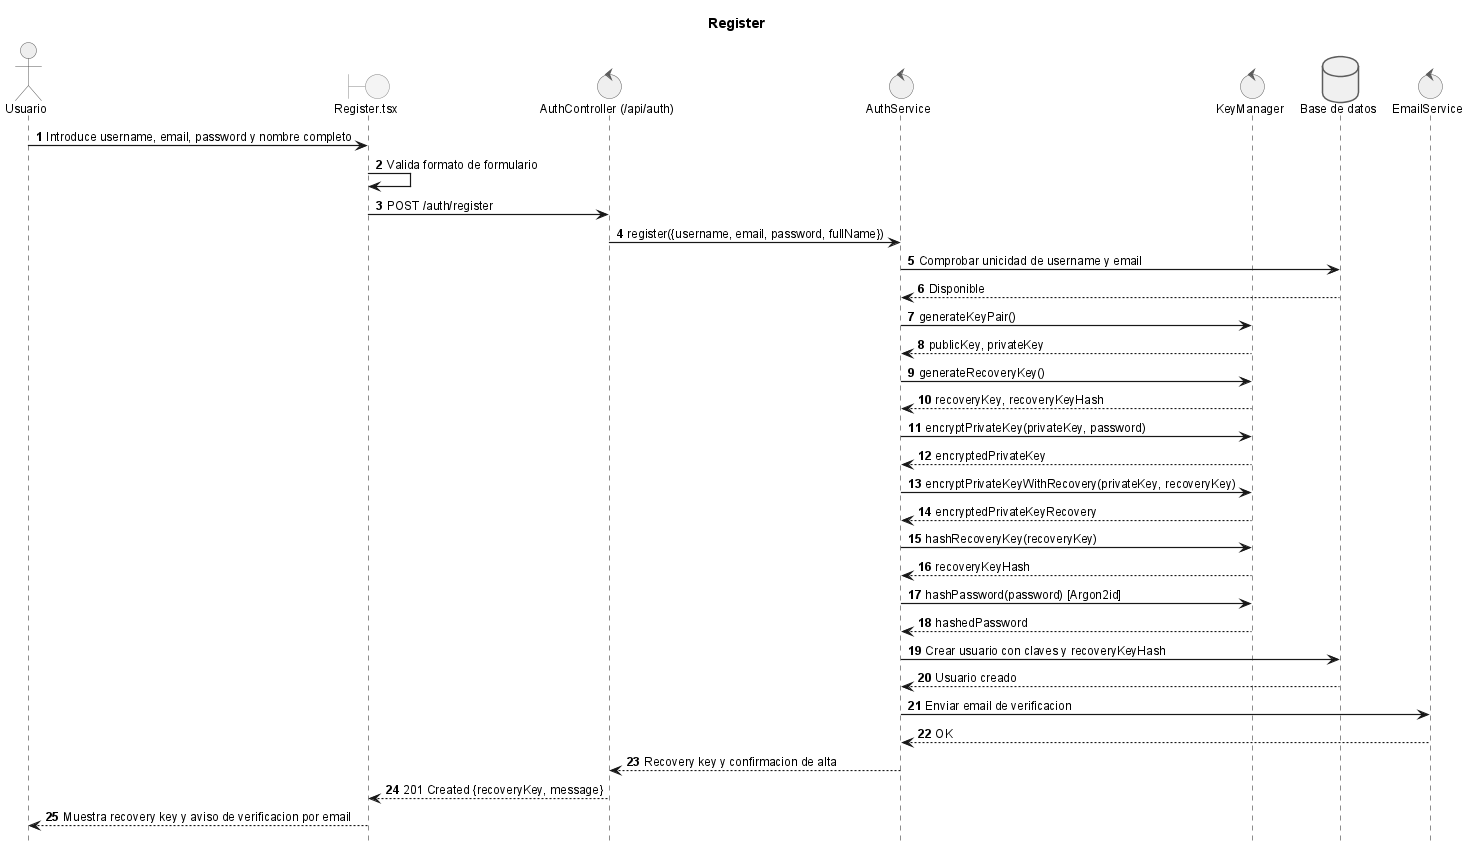
\includegraphics[width=0.92\textwidth]{diagramas/seq-register.png}
    \caption{Diagrama de secuencia del proceso de registro y verificación de correo}
    \label{fig:seq-register-mem}
\end{figure}

El flujo de subida de un nuevo documento (Figura~\ref{fig:seq-upload-mem}) concentra el patrón prepare/confirm descrito anteriormente: validación, cifrado, subida a IPFS, firma wallet y confirmación.

\begin{figure}[H]
    \centering
    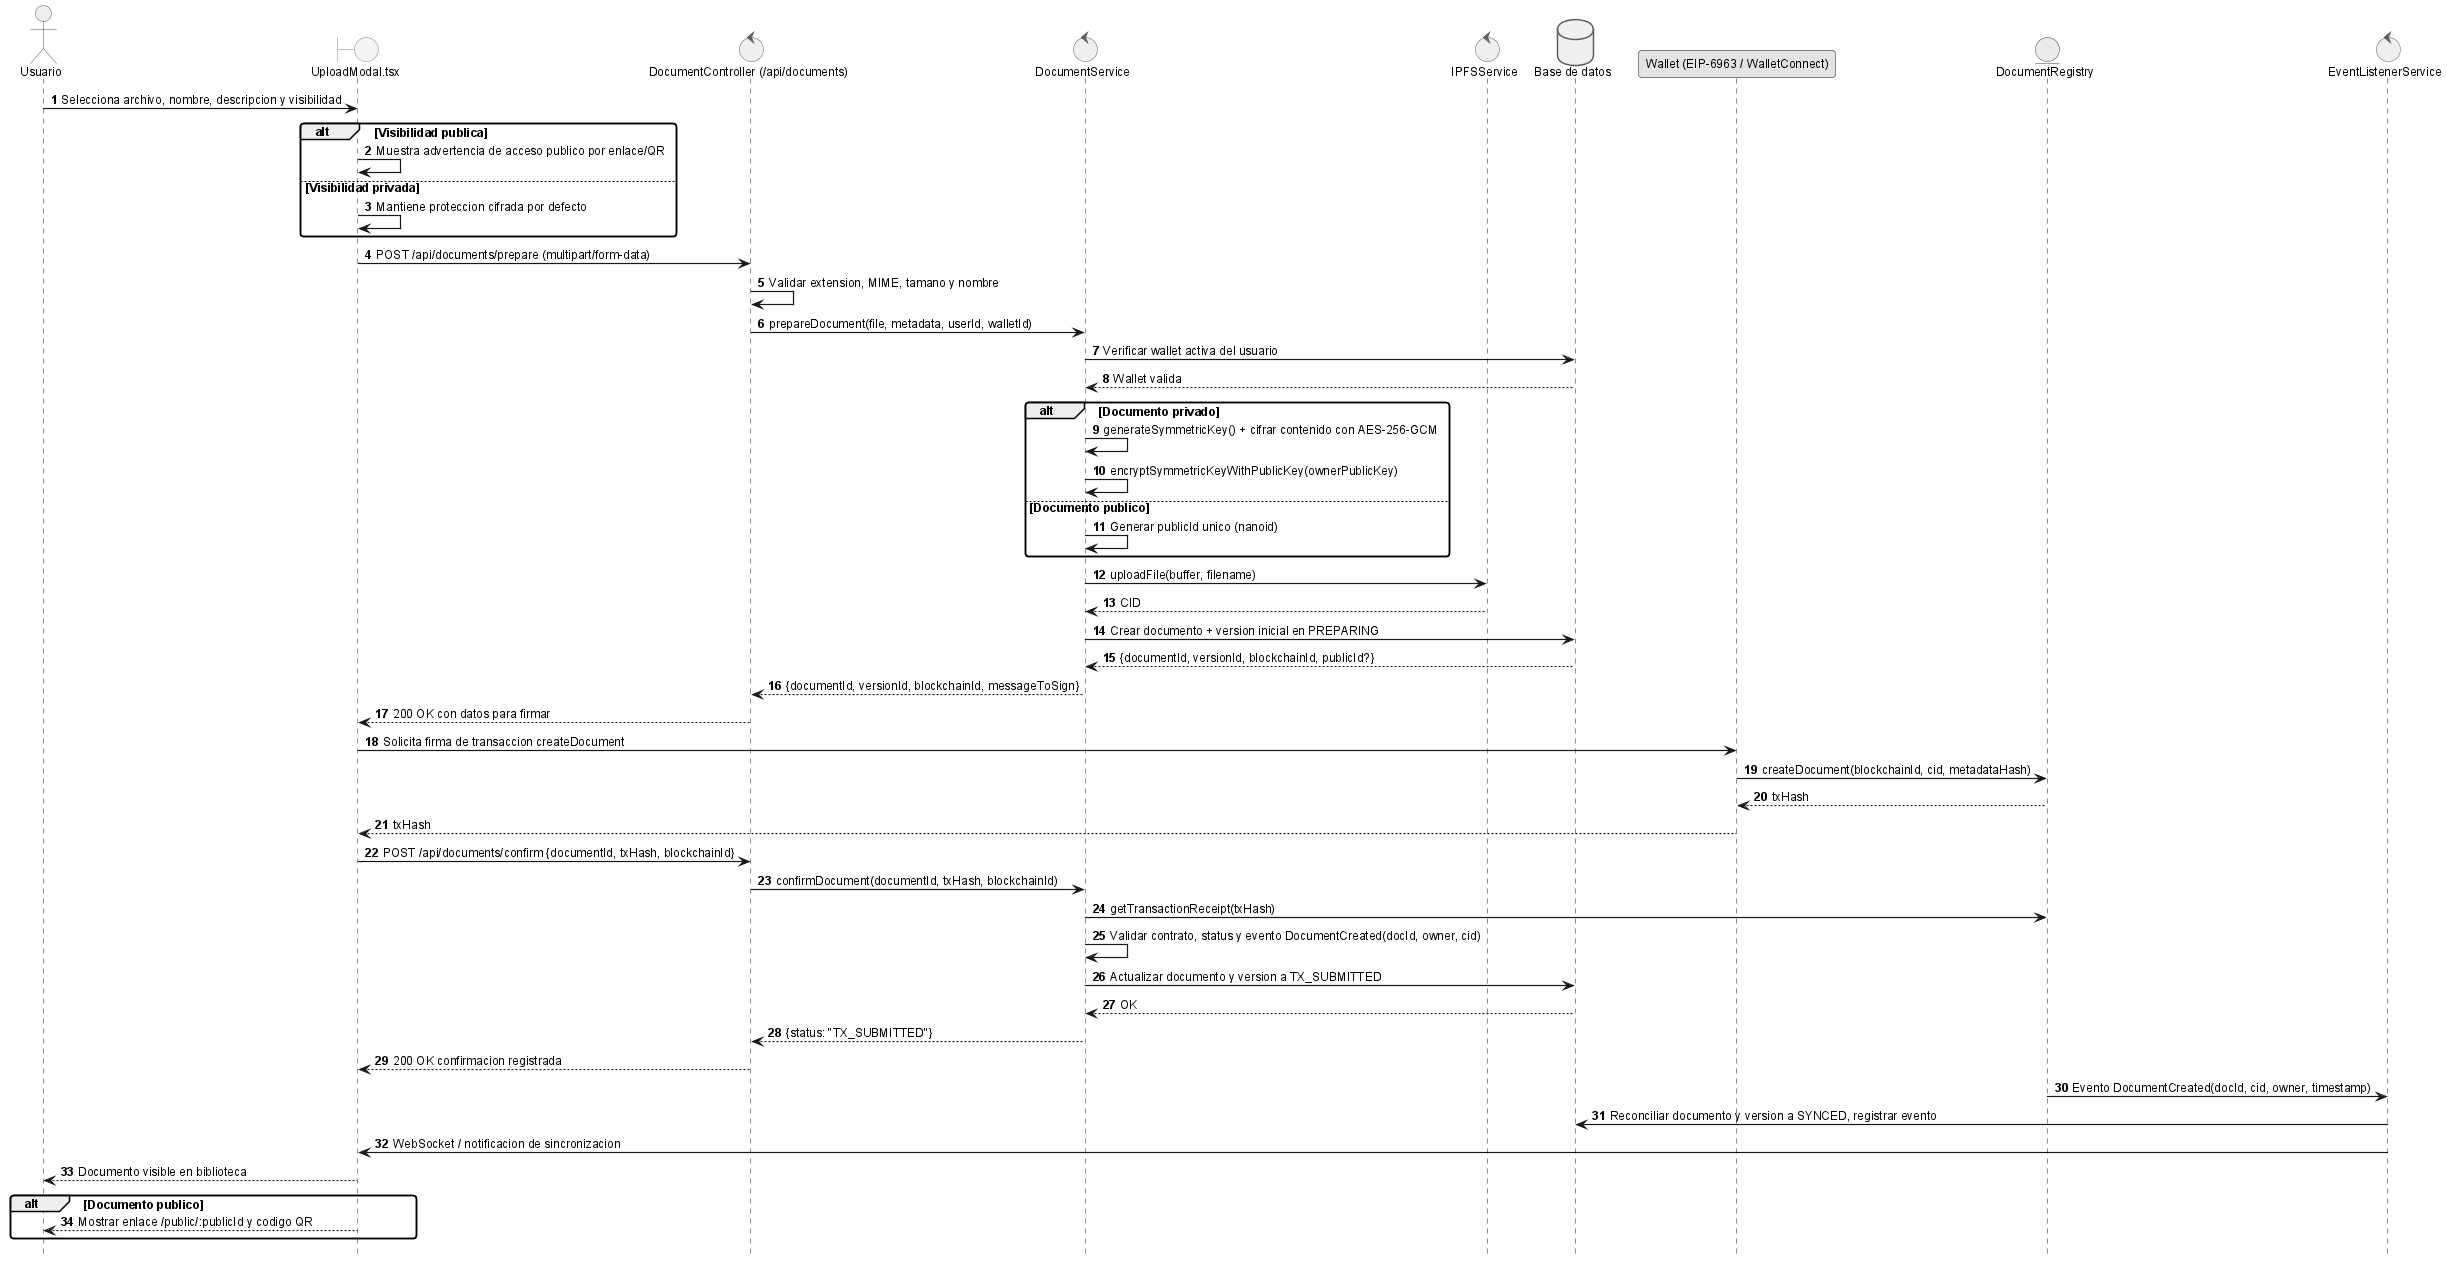
\includegraphics[width=0.92\textwidth]{diagramas/seq-upload.png}
    \caption{Diagrama de secuencia del flujo de subida de documento con integración IPFS y blockchain}
    \label{fig:seq-upload-mem}
\end{figure}

La Figura~\ref{fig:seq-share-mem} ilustra el flujo de compartición: la API registra la relación off-chain y emite el evento on-chain de actualización de permisos.

\begin{figure}[H]
    \centering
    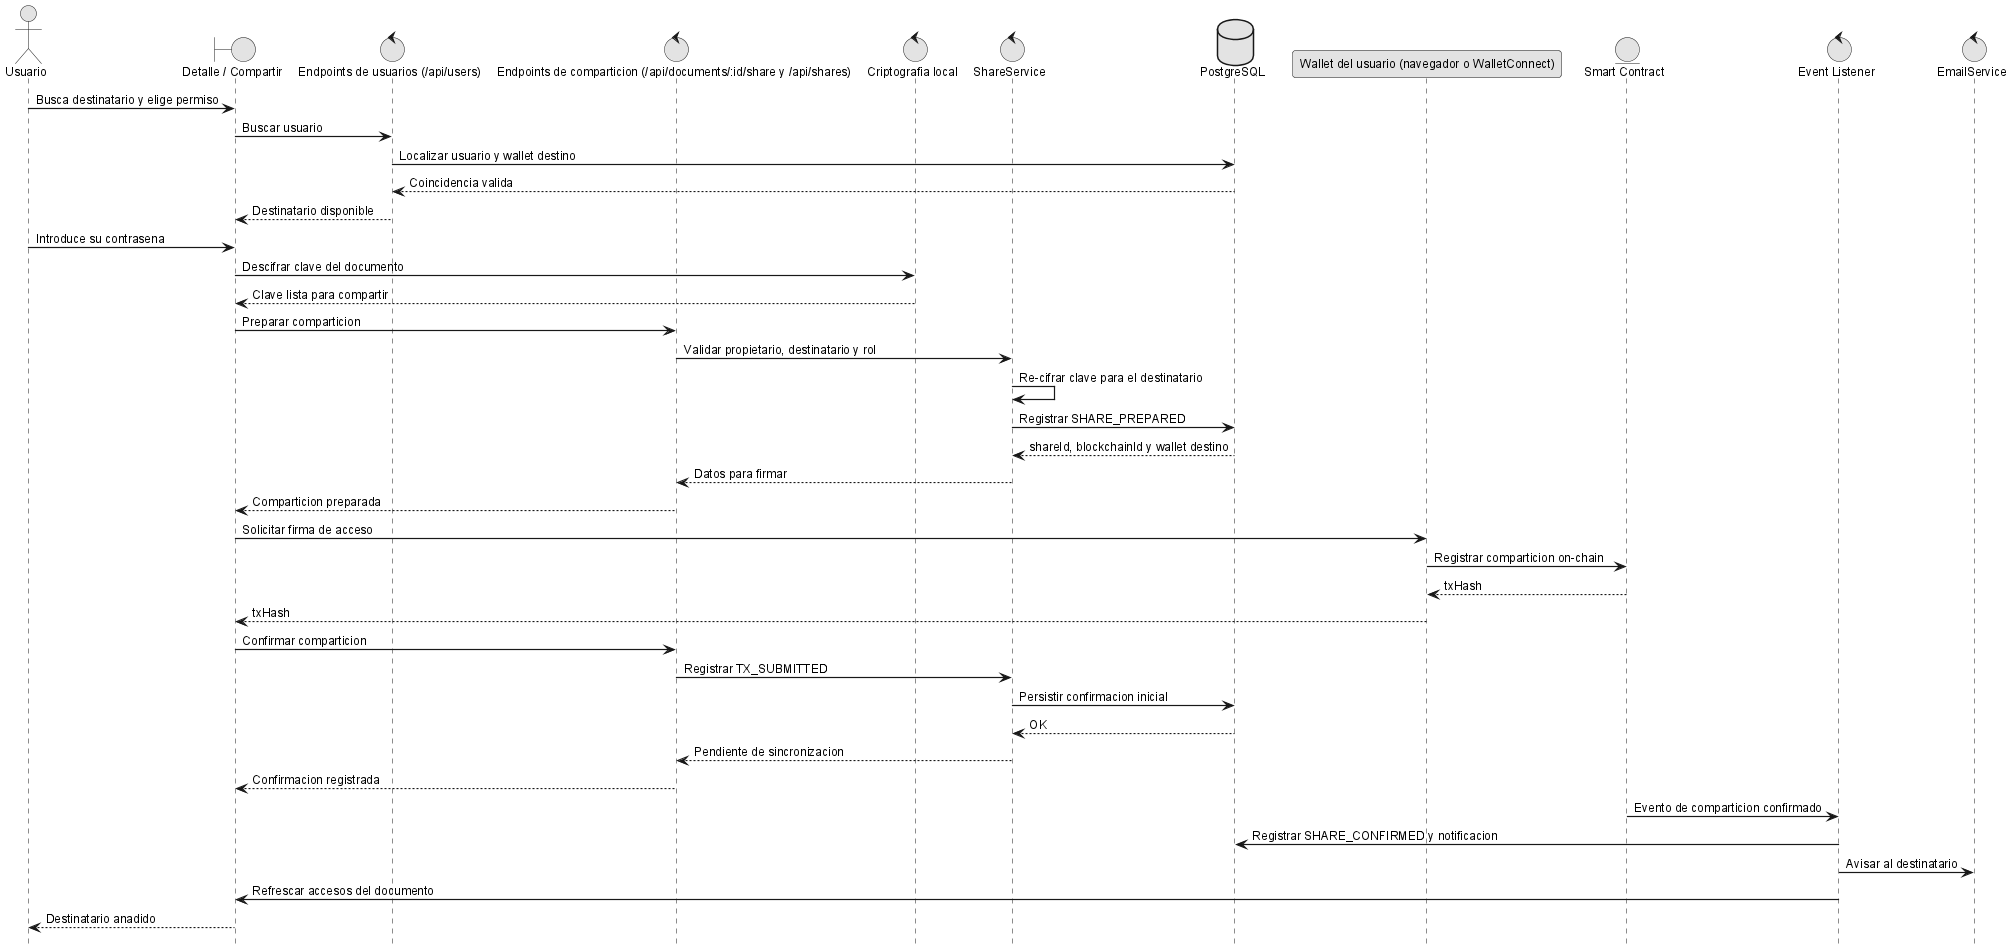
\includegraphics[width=0.92\textwidth]{diagramas/seq-share.png}
    \caption{Diagrama de secuencia del flujo de compartición de documento con tercero}
    \label{fig:seq-share-mem}
\end{figure}

La firma digital (Figura~\ref{fig:seq-sign-mem}) requiere que el usuario tenga wallet activa. El diagrama muestra la preparación de la operación por parte del backend, la solicitud de firma al cliente y el registro de la evidencia on-chain.

\begin{figure}[H]
    \centering
    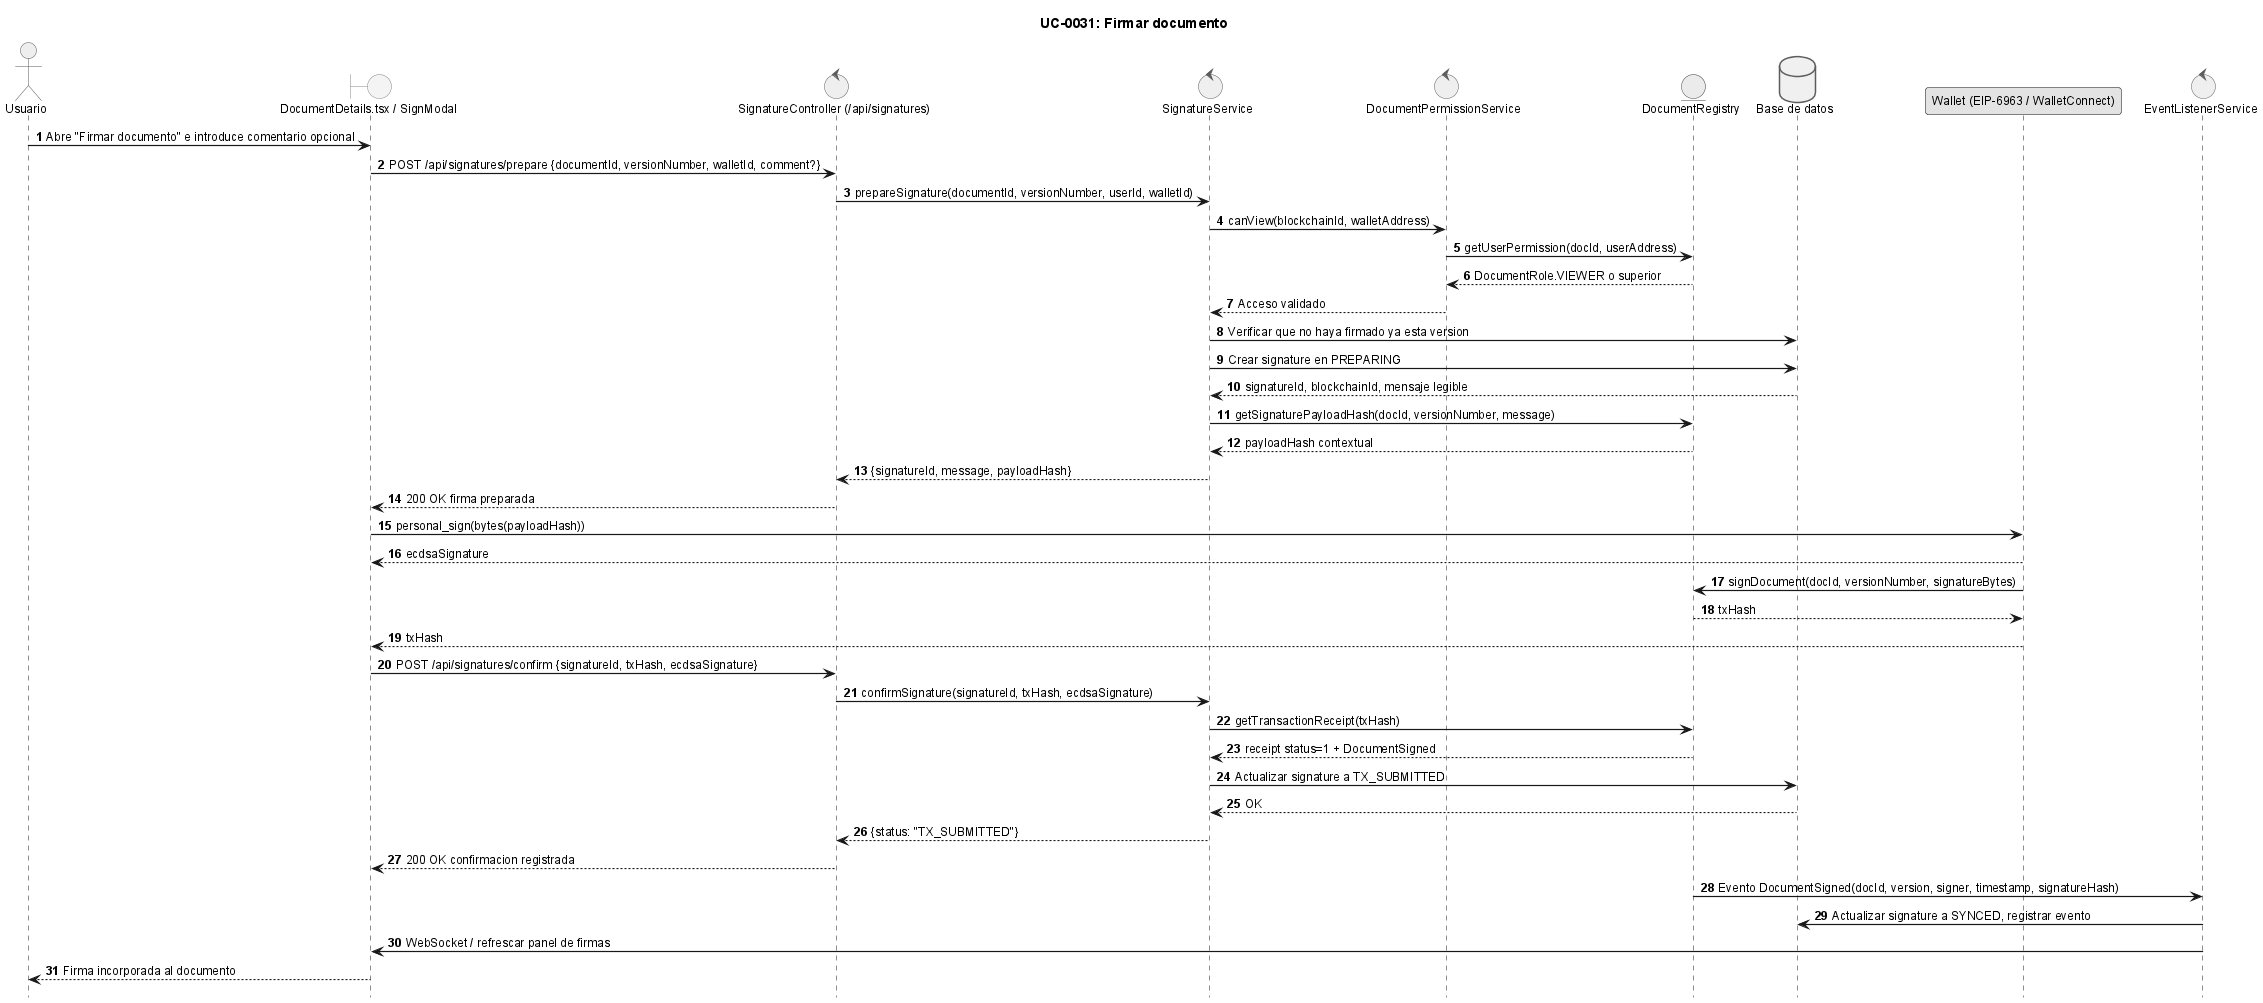
\includegraphics[width=0.92\textwidth]{diagramas/seq-sign.png}
    \caption{Diagrama de secuencia de la firma digital de documento con wallet y registro blockchain}
    \label{fig:seq-sign-mem}
\end{figure}

La Figura~\ref{fig:seq-2fa-mem} muestra la configuración del segundo factor TOTP: generación del secreto, presentación del código QR y verificación del código inicial antes de activar el mecanismo.

\begin{figure}[H]
    \centering
    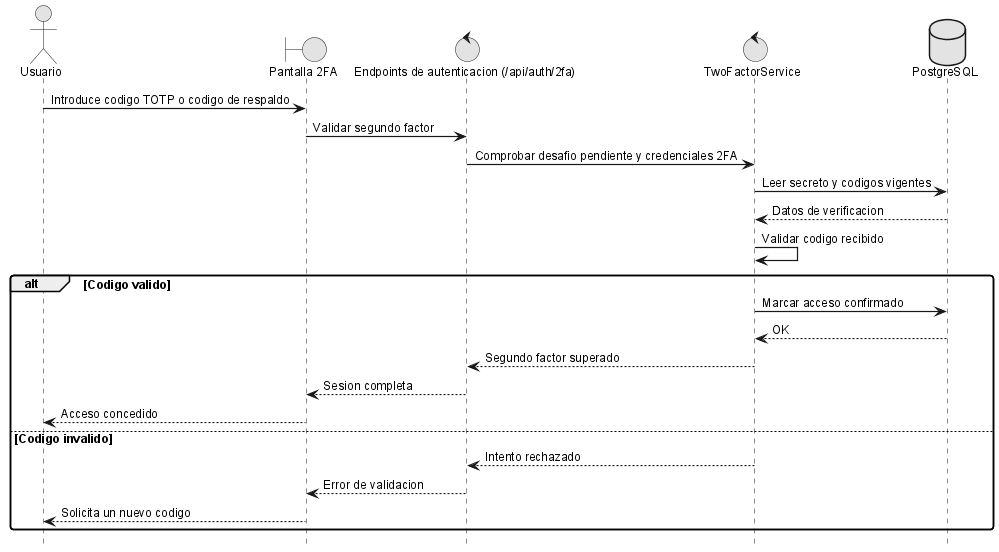
\includegraphics[width=0.88\textwidth]{diagramas/seq-2fa.png}
    \caption{Diagrama de secuencia de la configuración del segundo factor de autenticación TOTP}
    \label{fig:seq-2fa-mem}
\end{figure}

\subsection{Tecnologías e implementación}

\subsubsection{Organización del código}

La implementación se distribuye en cuatro bloques de trabajo principales dentro del repositorio: frontend, backend, contratos inteligentes y anexos/documentación. Esta organización favorece el aislamiento por responsabilidad y permite mantener ciclos de compilación y validación diferentes según el tipo de componente. En el backend se separan controladores, servicios, configuración, utilidades criptográficas y acceso a datos. En el frontend se distinguen páginas, componentes, contextos, rutas y librerías de integración con blockchain.

\subsubsection{Tecnologías seleccionadas}

La elección del stack responde a criterios de madurez, familiaridad académica y compatibilidad entre capas. React y TypeScript facilitan una interfaz tipada y razonablemente mantenible. Express proporciona una API sencilla y bien conocida. Prisma reduce fricción en el acceso a PostgreSQL. Hardhat resuelve el ciclo local de despliegue y prueba del contrato. Docker Compose aporta un entorno reproducible para toda la solución. IPFS se integra mediante un nodo Kubo autoalojado, lo que mantiene el control operativo de la persistencia sin depender de un tercero.

\begin{table}[H]
    \centering
    \small
    \begin{tabular}{|p{3.2cm}|p{3.5cm}|p{6.5cm}|}
    \hline
    \textbf{Bloque} & \textbf{Tecnología} & \textbf{Motivo principal de adopción} \\
    \hline
    Frontend & React, Vite, TypeScript & Rapidez de desarrollo, tipado estático y ecosistema maduro de componentes y rutas. \\
    \hline
    Backend & Express, Prisma, Node.js & Separación clara de servicios, integración con PostgreSQL y buena capacidad de prueba. \\
    \hline
    Blockchain & Solidity, Hardhat, Ethers & Despliegue local reproducible y contrato verificable para evidencia documental. \\
    \hline
    Persistencia externa & PostgreSQL, IPFS & Reparto entre consulta operativa y almacenamiento direccionado por contenido. \\
    \hline
    Operación & Docker Compose, Nginx, Postfix & Entorno reproducible, publicación del frontend y correo transaccional desacoplado. \\
    \hline
    \end{tabular}
    \caption{Tecnologías principales y criterio de selección}
    \label{tab:tecnologias-seleccion}
\end{table}

\subsubsection{Gestión de configuración}

La configuración del sistema se concentra en variables de entorno que permiten parametrizar el endpoint del nodo IPFS autoalojado, definir la URL de blockchain, fijar credenciales SMTP, ajustar límites de petición y establecer secretos de autenticación. Este enfoque reduce las dependencias rígidas incrustadas en código y aproxima la solución a una operativa realista, donde el mismo software puede cambiar de entorno sin ser reescrito.

\subsubsection{Integración entre operación y evidencia}

Una parte significativa de la implementación se ha dedicado a resolver la relación entre el estado operativo y el estado verificable. El backend no solo ejecuta lógica de negocio; también traduce entre el lenguaje de la interfaz, la estructura relacional, los CIDs de IPFS y las transacciones del contrato. Esa labor de coordinación se observa con claridad en operaciones como compartir, firmar o transferir propiedad, donde la interfaz necesita una respuesta inmediata y la evidencia blockchain puede consolidarse unos instantes más tarde.

\subsection{Aspectos de seguridad}

\subsubsection{Protección de datos y minimización}

El sistema trata datos identificativos básicos, credenciales, wallets, eventos de actividad y documentos cuyo contenido puede ser sensible. Por ello se ha seguido un criterio de minimización: cada capa conserva la información estrictamente necesaria para cumplir su responsabilidad. No se publica en blockchain información personal detallada. Tampoco se utiliza IPFS como depósito indiscriminado de metadatos operativos. El contenido privado recibe un tratamiento diferente al contenido que el usuario decide publicar mediante enlace compartible.

\subsubsection{Modelo criptográfico}

La protección del contenido privado se apoya en AES-256-GCM, de modo que el documento se cifra antes de conservarse fuera del backend. Las claves simétricas asociadas a documento o versión no se exponen en cadena. Se protegen fuera de ella mediante mecanismos asimétricos y se reutilizan de forma controlada cuando la operación exige compartir o transferir acceso. Las contraseñas se endurecen con Argon2id y el acceso ordinario a la cuenta puede reforzarse con TOTP.

\begin{table}[H]
    \centering
    \small
    \begin{tabular}{|p{3.6cm}|p{3.6cm}|p{5.9cm}|}
    \hline
    \textbf{Activo protegido} & \textbf{Mecanismo} & \textbf{Propósito} \\
    \hline
    Contraseña de usuario & Argon2id & Dificultar ataques offline y endurecer el almacenamiento de credenciales. \\
    \hline
    Documento privado & AES-256-GCM & Garantizar confidencialidad e integridad del binario almacenado. \\
    \hline
    Clave simétrica & Protección asimétrica fuera de cadena & Permitir acceso controlado por usuario y compartir sin revelar el material en claro. \\
    \hline
    Sesión de usuario & JWT y controles de expiración & Mantener autenticación operativa sin delegar toda la identidad en la wallet. \\
    \hline
    Operación crítica & Firma con wallet & Vincular el acto on-chain con el usuario que lo autoriza. \\
    \hline
    \end{tabular}
    \caption{Controles de seguridad principales aplicados en el sistema}
    \label{tab:controles-seguridad}
\end{table}

\subsubsection{Autenticación, autorización y privilegio mínimo}

El acceso ordinario se realiza mediante usuario o correo y contraseña. La wallet no se utiliza como mecanismo principal de entrada en la interfaz habitual, sino como instrumento de firma para operaciones que deben quedar registradas on-chain. La autorización combina un modelo de roles globales para administración con un modelo de permisos documentales por recurso. Esta doble capa permite que la sesión autenticada no baste por sí sola para ejecutar cualquier acción sobre cualquier documento.

\subsubsection{Privacidad, publicación pública y consideraciones normativas}

La existencia de documentos públicos obliga a distinguir entre protección por defecto y publicación deliberada. Cuando el usuario activa la visibilidad pública, el documento deja de tratarse como binario privado y pasa a exponerse mediante \texttt{publicId}. Esa transformación forma parte del comportamiento previsto y se acompaña de una diferenciación visible en la interfaz. Desde el punto de vista normativo, esta distinción resulta relevante porque no toda operación documental implica el mismo tratamiento de datos ni la misma expectativa de reserva.

\subsubsection{Mejora continua y seguimiento operativo}

La seguridad del sistema no se agota en las decisiones de diseño inicial. La actualización de dependencias, la vigilancia de errores de sincronización, la revisión del estado de servicios y la detección de incidencias de acceso a IPFS o blockchain forman parte del mantenimiento necesario para que el prototipo siga siendo defendible a lo largo del tiempo. En este sentido, la arquitectura desacoplada facilita aislar problemas y corregirlos sin alterar la totalidad del sistema.

\subsection{Descripción de las pruebas}

\subsubsection{Estrategia general de validación}

La validación del proyecto se ha sostenido en tres niveles complementarios. El primero corresponde a pruebas automatizadas de backend y contratos. El segundo cubre pruebas funcionales de sistema orientadas a recorridos completos de usuario. El tercero se apoya en capturas y manuales que permiten contrastar que la implementación visible coincide con lo descrito en la documentación académica. Esta combinación evita depender exclusivamente de un único tipo de evidencia.

\subsubsection{Pruebas automatizadas}

La guía de testing del proyecto documenta 207 pruebas automatizadas. De ellas, 105 se centran en backend y lógica de servicios, mientras que 102 verifican el contrato inteligente y su comportamiento ante condiciones normales, casos límite y mecanismos de seguridad. La distribución es relevante porque muestra que la validación no se ha concentrado solo en una capa de la solución.

\begin{table}[H]
    \centering
    \small
    \begin{tabular}{|p{4cm}|p{2cm}|p{6.8cm}|}
    \hline
    \textbf{Bloque de prueba} & \textbf{Cantidad} & \textbf{Cobertura representativa} \\
    \hline
    Blockchain queries & 45 & Recuperación de documentos, versiones, permisos, firmas y listados por usuario. \\
    \hline
    Permisos documentales & 38 & Roles VIEWER/EDITOR/OWNER, compartición, revocación y errores de acceso. \\
    \hline
    Cifrado y utilidades criptográficas & 14 & Roundtrip de AES-256-GCM, IV, auth tags, protección de claves y validaciones. \\
    \hline
    Integración backend & 8 & Ciclos completos de cifrado, IPFS, compartición, transferencias y concurrencia. \\
    \hline
    Contrato \texttt{DocumentRegistry} & 102 & Creación, versionado, firma, permisos, archivado, pausa y seguridad del contrato. \\
    \hline
    \end{tabular}
    \caption{Distribución principal de las pruebas automatizadas documentadas}
    \label{tab:pruebas-automatizadas}
\end{table}

\subsubsection{Validación funcional del sistema}

Las guías de pruebas del sistema complementan la automatización con recorridos completos que implican interfaz, backend, wallet y persistencia. Entre los escenarios contemplados se encuentran el registro de usuario, el bloqueo de acceso hasta la verificación del correo, el reenvío de mensajes de confirmación, la autenticación, la subida documental, la creación de nuevas versiones, la firma, la compartición, la transferencia de propiedad, la gestión de wallets, la auditoría y la verificación pública. La amplitud de estos recorridos permite comprobar la integración real entre componentes que, de otro modo, podrían validarse solo de manera aislada.

\begin{table}[H]
    \centering
    \small
    \begin{tabular}{|p{4cm}|p{8.8cm}|}
    \hline
    \textbf{Escenario funcional} & \textbf{Comprobación principal} \\
    \hline
    Registro e inicio de sesión & Alta de usuario, confirmación de la \textit{Recovery Key}, bloqueo hasta la verificación del correo, reenvío del mensaje y acceso posterior con control de rol. \\
    \hline
    Subida documental & Generación de CID, confirmación de transacción y visibilidad del documento creado. \\
    \hline
    Versionado & Creación de versión nueva, historial y activación de versión operativa. \\
    \hline
    Firma digital & Asociación de wallet, timestamp, comentario y rastro on-chain verificable. \\
    \hline
    Compartición y transferencia & Cambio de permisos, revocación y traspaso de titularidad entre usuarios. \\
    \hline
    Verificación pública & Consulta de enlaces públicos y validación de integridad sin autenticación. \\
    \hline
    \end{tabular}
    \caption{Escenarios funcionales representativos validados mediante guías del sistema}
    \label{tab:escenarios-funcionales}
\end{table}

\subsubsection{Evidencia visual de la validación}

La validación del prototipo se apoya también en capturas de la interfaz real generadas para el Anexo V. Estas capturas no cumplen únicamente una función estética. Permiten demostrar la existencia de páginas, diálogos y recorridos descritos en la documentación y sirven como evidencia de correspondencia entre diseño, implementación y operación. La Figura~\ref{fig:auditoria-publica} muestra una de las vistas más representativas en este sentido.

\begin{figure}[H]
    \centering
    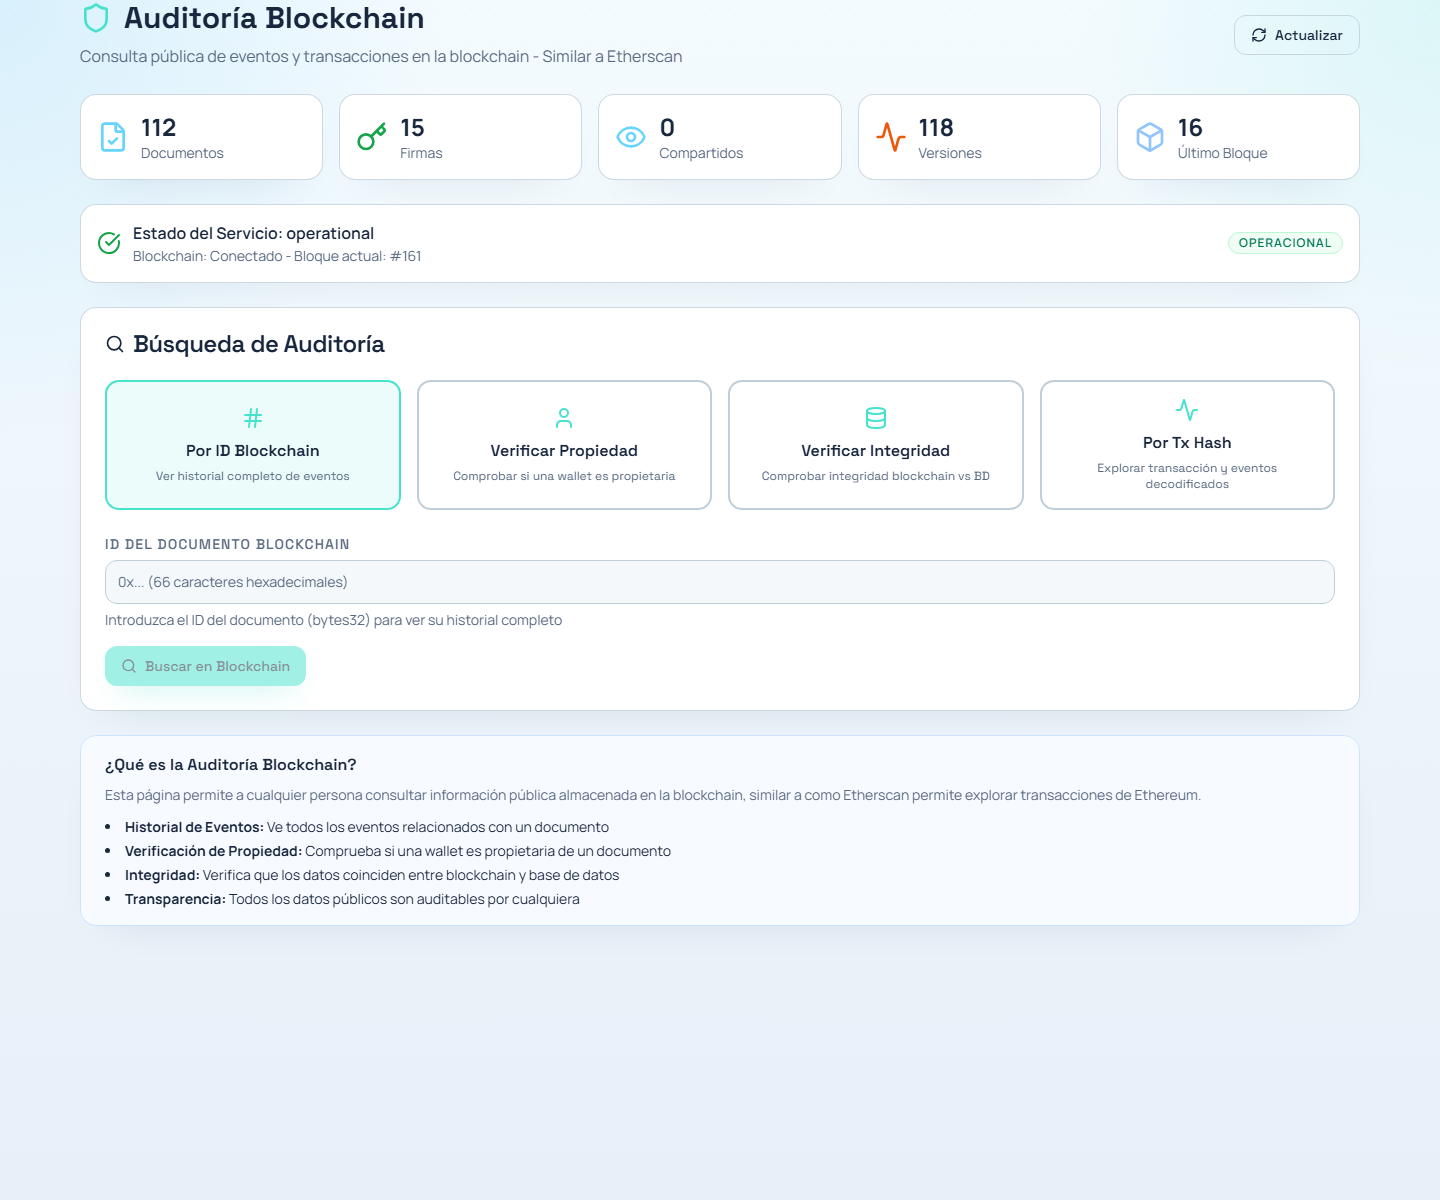
\includegraphics[width=0.9\textwidth]{capturas-ui/public-audit-page.png}
    \caption{Pantalla de auditoría pública y verificación de evidencias}
    \label{fig:auditoria-publica}
\end{figure}

\subsection{Gestión del proyecto}

\subsubsection{Estructura de trabajo}

El desarrollo del proyecto se ha organizado de forma incremental, separando claramente los cuatro grandes ámbitos de trabajo: frontend, backend, contratos inteligentes y documentación académica. Esta división no solo ordena el repositorio, sino que facilita un ritmo de trabajo donde cada bloque puede evolucionar sin bloquear por completo a los demás. A la vez, obliga a mantener puntos de integración frecuentes, especialmente entre servicios backend, contrato y experiencia de usuario.

\begin{table}[H]
    \centering
    \small
    \begin{tabular}{|p{3cm}|p{3.3cm}|p{6.3cm}|}
    \hline
    \textbf{Bloque de trabajo} & \textbf{Contenido principal} & \textbf{Función dentro del proyecto} \\
    \hline
    Frontend & SPA en React, rutas, componentes y capturas & Materializa la experiencia de usuario y la operativa documental visible. \\
    \hline
    Backend & API, servicios, cifrado, notificaciones y acceso a datos & Coordina la lógica de negocio y la integración entre persistencias. \\
    \hline
    Smart contracts & Contrato Solidity, scripts y pruebas & Aporta la capa de evidencia y control on-chain. \\
    \hline
    Documentación & Anexos, memoria, diagramas y guías & Recoge especificación, diseño, validación y defensa del trabajo realizado. \\
    \hline
    \end{tabular}
    \caption{Bloques de trabajo que estructuran el desarrollo de DocumentChain}
    \label{tab:bloques-trabajo}
\end{table}

\subsubsection{Gestión por fases e iteraciones}

La planificación detallada del Anexo III muestra que el proyecto se ha conducido siguiendo una lógica próxima al Proceso Unificado. Las primeras iteraciones se dedicaron a entender el dominio, estudiar soluciones existentes, delimitar alcance y fijar el stack tecnológico. Las siguientes se centraron en consolidar requisitos, diagramas y diseño. Solo después se abordó la implementación progresiva del backend, del contrato, del frontend y de las pruebas integradas. Esta secuencia ha sido útil porque evita construir demasiado pronto sobre decisiones insuficientemente justificadas.

Durante la construcción, la gestión iterativa ha permitido cerrar incrementos funcionales con sentido propio: autenticación y registro, subida documental, cifrado, integración IPFS, versionado, compartición, firma, auditoría, administración y despliegue. Ese orden de trabajo reduce el riesgo de acumular componentes inconexos y facilita que cada avance pueda probarse sobre un caso de uso reconocible.

\subsubsection{Gestión de documentación y evidencia}

Una particularidad del proyecto es que la documentación no se ha producido únicamente al final. Los anexos, las guías de pruebas, los manuales de usuario y la propia memoria se han ido alimentando conforme maduraban el análisis y la implementación. Esta práctica tiene un valor claro desde el punto de vista académico: la memoria no depende de reconstruir retrospectivamente decisiones antiguas, sino que puede apoyarse en artefactos ya consolidados durante el desarrollo.

Del mismo modo, la evidencia del proyecto se conserva en varios formatos complementarios. Los diagramas sintetizan arquitectura y diseño. Las capturas demuestran la existencia de la interfaz real. Las pruebas automatizadas aportan validación repetible. Y la documentación de arranque y operación permite reproducir el entorno. La combinación de estas fuentes fortalece la trazabilidad entre lo diseñado, lo implementado y lo finalmente defendido.

\subsubsection{Gestión técnica del repositorio}

El repositorio se ha utilizado como espacio de integración de código, scripts de arranque, composición de contenedores, documentación y activos gráficos. Esta concentración simplifica la reproducibilidad del trabajo, porque el lector o evaluador dispone en un único entorno del software, de su infraestructura y de la documentación que lo explica. Además, la presencia de ficheros de ejemplo para variables de entorno, guías de arranque y scripts de apoyo reduce la dependencia de conocimiento tácito durante la puesta en marcha.

\subsubsection{Planificación temporal}

La estimación del proyecto se ha apoyado en puntos de caso de uso ajustados. El Anexo III desarrolla esta metodología y calcula tanto los factores de complejidad técnica como los factores del entorno. El resultado obtenido se cifra en 442 UCP, valor que la herramienta EZEstimate traduce a una estimación próxima a 1.500 horas de trabajo. Esta cifra no debe leerse como una verdad absoluta, sino como una referencia razonada para ordenar el esfuerzo del proyecto.

\begin{figure}[H]
    \centering
    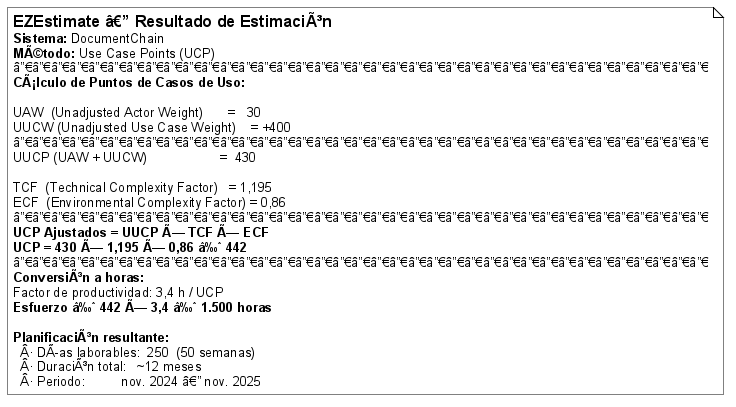
\includegraphics[width=0.83\textwidth]{diagramas/ezestimate.png}
    \caption{Resultado de estimación UCP mediante la herramienta EZEstimate}
    \label{fig:ezestimate-memoria}
\end{figure}

\begin{table}[H]
    \centering
    \small
    \begin{tabular}{|p{6.2cm}|p{4cm}|}
    \hline
    \textbf{Parámetro} & \textbf{Valor} \\
    \hline
    Puntos de caso de uso sin ajustar (UUCP) & 430 \\
    \hline
    Factor de complejidad técnica (TCF) & 1,195 \\
    \hline
    Factor del entorno (ECF) & 0,86 \\
    \hline
    Puntos de caso de uso ajustados (UCP) & 442 \\
    \hline
    Estimación global de esfuerzo & 1.500 horas \\
    \hline
    Ventana temporal estimada & Diciembre de 2025 a mayo de 2026 \\
    \hline
    \end{tabular}
    \caption{Resumen de la estimación empleada para el proyecto}
    \label{tab:estimacion-memoria}
\end{table}

La planificación se ha alineado con las fases del Proceso Unificado. Inicio y Elaboración concentran definición de alcance, requisitos, arquitectura y documentación base. Construcción agrupa el grueso de la implementación y de las pruebas. Transición se centra en despliegue, validación final, cierre documental y preparación de la defensa. Esta secuencia no solo ordena el trabajo; también explica por qué los anexos y la memoria evolucionan en paralelo al producto software y no como actividad residual del cierre.

\begin{table}[H]
    \centering
    \small
    \begin{tabular}{|p{3cm}|p{3cm}|p{3cm}|p{3.2cm}|}
    \hline
    \textbf{Fase} & \textbf{Peso temporal} & \textbf{Horas aproximadas} & \textbf{Enfoque principal} \\
    \hline
    Inicio & Breve & 90 & Alcance, actores, objetivos y planificación inicial. \\
    \hline
    Elaboración & Moderado & 210 & Requisitos, arquitectura, smart contract y anexos de análisis. \\
    \hline
    Construcción & Mayoritario & 1.020 & Implementación incremental de backend, frontend, blockchain, IPFS y pruebas. \\
    \hline
    Transición & Acotado & 180 & Despliegue, validación final, memoria y defensa. \\
    \hline
    \end{tabular}
    \caption{Distribución resumida del esfuerzo por fases del proyecto}
    \label{tab:fases-proyecto}
\end{table}

\begin{figure}[H]
    \centering
    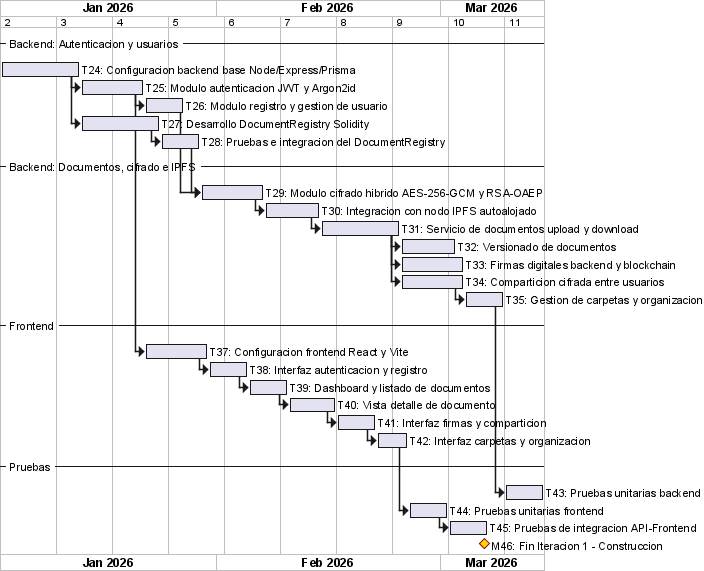
\includegraphics[width=0.96\textwidth]{diagramas/gantt-const1.png}
    \caption{Extracto del cronograma de trabajo para la fase de construcción}
    \label{fig:gantt-const1-memoria}
\end{figure}

Los diagramas de Gantt por iteración desglosan la distribución real del trabajo a lo largo del proyecto. Las figuras siguientes los presentan organizados por fase del proceso unificado.

\textbf{Fase de Inicio.} La primera iteración (Figura~\ref{fig:gantt-inicio1-mem}) cubre la toma de requisitos, selección tecnológica y configuración del entorno base. La segunda (Figura~\ref{fig:gantt-inicio2-mem}) cierra la fase con la arquitectura conceptual y el primer prototipo de contrato.

\begin{figure}[H]
    \centering
    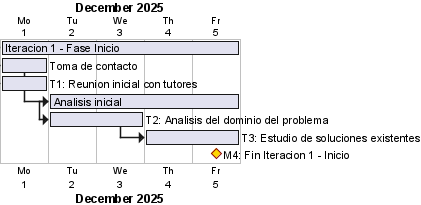
\includegraphics[width=0.96\textwidth]{diagramas/gantt-inicio1.png}
    \caption{Diagrama de Gantt de la primera iteración de la fase de Inicio}
    \label{fig:gantt-inicio1-mem}
\end{figure}

\begin{figure}[H]
    \centering
    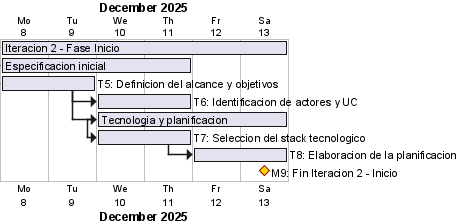
\includegraphics[width=0.96\textwidth]{diagramas/gantt-inicio2.png}
    \caption{Diagrama de Gantt de la segunda iteración de la fase de Inicio}
    \label{fig:gantt-inicio2-mem}
\end{figure}

\textbf{Fase de Elaboración.} La primera iteración (Figura~\ref{fig:gantt-elab1-mem}) abarca el diseño de persistencia y el núcleo del contrato inteligente. La segunda (Figura~\ref{fig:gantt-elab2-mem}) cubre la integración IPFS y los flujos principales de la API.

\begin{figure}[H]
    \centering
    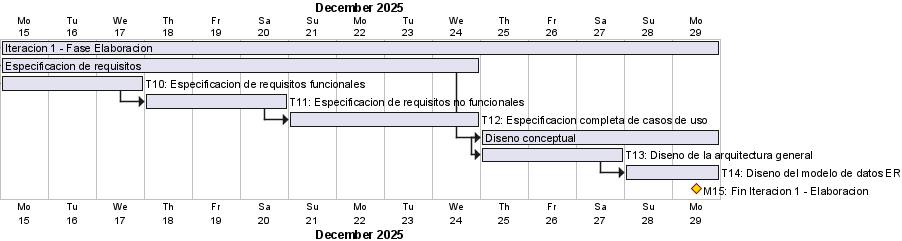
\includegraphics[width=0.96\textwidth]{diagramas/gantt-elab1.png}
    \caption{Diagrama de Gantt de la primera iteración de la fase de Elaboración}
    \label{fig:gantt-elab1-mem}
\end{figure}

\begin{figure}[H]
    \centering
    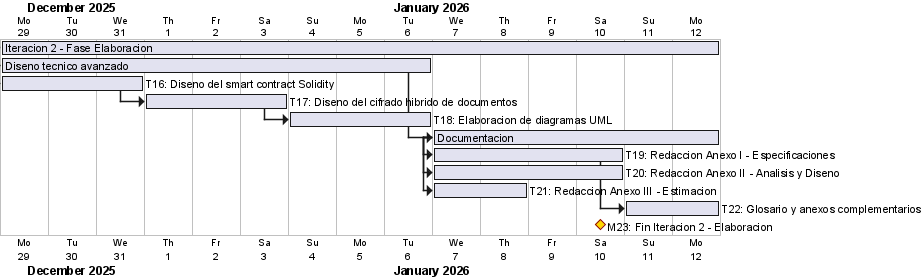
\includegraphics[width=0.96\textwidth]{diagramas/gantt-elab2.png}
    \caption{Diagrama de Gantt de la segunda iteración de la fase de Elaboración}
    \label{fig:gantt-elab2-mem}
\end{figure}

\textbf{Fase de Construcción.} La segunda iteración (Figura~\ref{fig:gantt-const2-mem}) incorpora firma, compartición, verificación pública y panel administrativo, completando el bloque ya mostrado en la Figura~\ref{fig:gantt-const1-memoria}.

\begin{figure}[H]
    \centering
    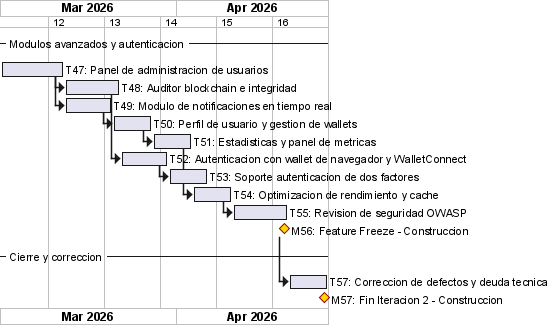
\includegraphics[width=0.96\textwidth]{diagramas/gantt-const2.png}
    \caption{Diagrama de Gantt de la segunda iteración de la fase de Construcción}
    \label{fig:gantt-const2-mem}
\end{figure}

\textbf{Fase de Transición.} La primera iteración (Figura~\ref{fig:gantt-trans1-mem}) abarca las pruebas de sistema y ajustes derivados. La segunda (Figura~\ref{fig:gantt-trans2-mem}) cubre la documentación académica, la revisión final y el despliegue de demostración.

\begin{figure}[H]
    \centering
    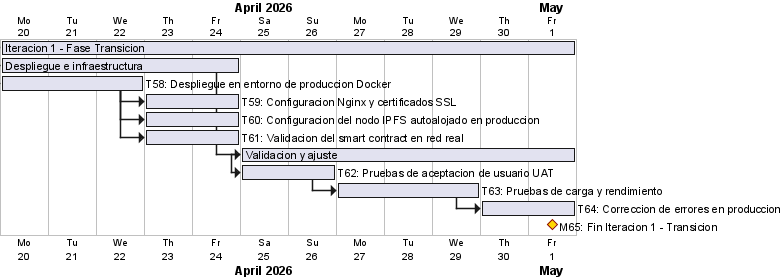
\includegraphics[width=0.96\textwidth]{diagramas/gantt-trans1.png}
    \caption{Diagrama de Gantt de la primera iteración de la fase de Transición}
    \label{fig:gantt-trans1-mem}
\end{figure}

\begin{figure}[H]
    \centering
    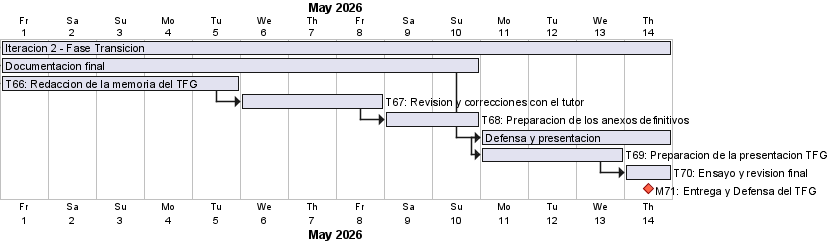
\includegraphics[width=0.96\textwidth]{diagramas/gantt-trans2.png}
    \caption{Diagrama de Gantt de la segunda iteración de la fase de Transición}
    \label{fig:gantt-trans2-mem}
\end{figure}

\subsection{Despliegue del sistema}

\subsubsection{Modelo de despliegue}

El proyecto se ha preparado para ejecutarse de forma reproducible mediante Docker Compose. La topología principal incluye cinco servicios: PostgreSQL, Hardhat, backend, frontend y Postfix. Esta decisión cumple una doble función. Facilita la puesta en marcha del sistema en otro equipo y, al mismo tiempo, permite defender una arquitectura que no depende de la ejecución manual dispersa de procesos sobre la máquina del desarrollador.

\begin{figure}[H]
    \centering
    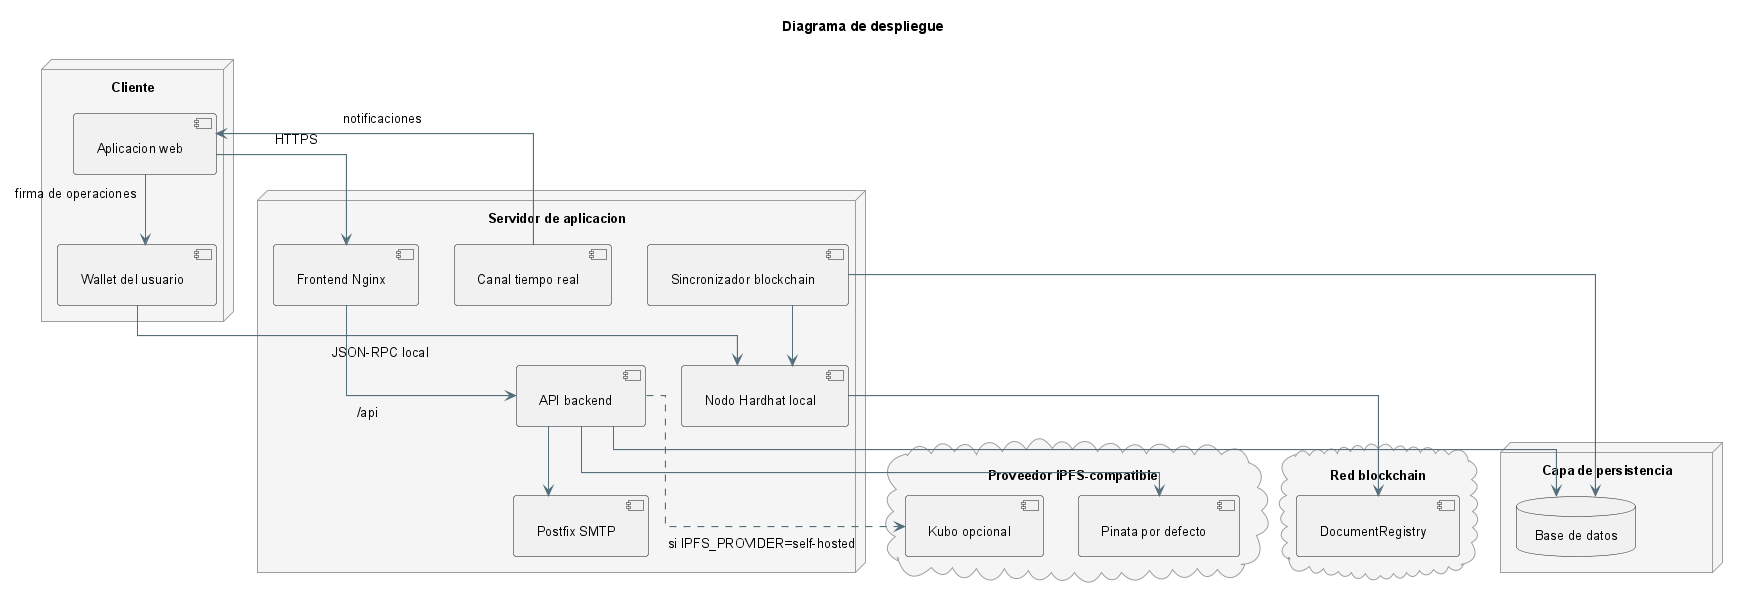
\includegraphics[width=0.9\textwidth]{diagramas/deployment.png}
    \caption{Esquema de despliegue del sistema mediante contenedores}
    \label{fig:deployment}
\end{figure}

\begin{table}[H]
    \centering
    \small
    \begin{tabular}{|p{2.9cm}|p{2.3cm}|p{6.9cm}|}
    \hline
    \textbf{Servicio} & \textbf{Puerto} & \textbf{Función principal} \\
    \hline
    PostgreSQL & 5433 & Persistencia relacional del estado operativo y de sincronización. \\
    \hline
    Hardhat & 8545 & Red EVM local para despliegue y validación del contrato. \\
    \hline
    Backend & 3000 & API REST, lógica de negocio, cifrado, notificaciones y coordinación de servicios. \\
    \hline
    Frontend & 5173 & Publicación de la SPA y acceso principal del usuario a la plataforma. \\
    \hline
    Postfix & 1587 & Entrega SMTP local y salida hacia relay o destinatario final. \\
    \hline
    \end{tabular}
    \caption{Servicios del despliegue base y su responsabilidad operativa}
    \label{tab:servicios-compose}
\end{table}

\subsubsection{Papel de Nginx en el frontend}

En el despliegue dockerizado, Nginx se utiliza para servir los archivos generados por Vite, resolver correctamente las rutas internas de la SPA y reenviar las peticiones API hacia el backend. Su inclusión no responde a una preferencia arbitraria, sino a la conveniencia de contar con un servidor HTTP ligero y estándar para una entrega seria del frontend. De este modo, la aplicación se presenta en un contexto más próximo a un despliegue real que a un simple servidor de desarrollo.

\subsubsection{Correo transaccional y operación SMTP}

El subsistema de correo se articula en dos planos. El backend genera el mensaje y decide el momento de envío. Postfix actúa como servidor SMTP de salida dentro del stack Docker. Esta separación mantiene el backend desacoplado del proveedor de entrega final y evita que la lógica de plantillas, notificaciones y recuperación de contraseña dependa de un servicio concreto. Durante la integración del proyecto se comprobó que la entrega MX directa no era el camino más fiable para el entorno disponible, por lo que se adoptó una estrategia basada en relay autenticado. Desde el punto de vista técnico, el flujo queda resumido como backend $\rightarrow$ Postfix $\rightarrow$ relay SMTP $\rightarrow$ destinatario final.

En términos operativos, esta decisión tiene una consecuencia relevante: el backend conserva una única forma de enviar correo, mientras que la variación de proveedor se concentra en la configuración de infraestructura. De ese modo, la aplicación puede mantenerse estable aunque cambie el proveedor de salida. La memoria recoge esta explicación porque forma parte del comportamiento entregable del sistema y no conviene relegarla a documentación de apoyo no presentada ante el tribunal.

\subsubsection{Diagnóstico y seguimiento del despliegue}

El despliegue no se considera completo por el mero hecho de que los contenedores arranquen. También es necesario verificar que la API responda, que la base de datos mantenga conectividad, que la red local de Hardhat esté disponible para operaciones firmadas, que IPFS acepte las subidas previstas y que la cola de correo no acumule incidencias silenciosas. En este sentido, el uso de Docker Compose facilita el diagnóstico porque cada servicio puede inspeccionarse de forma aislada mediante logs, estados y comprobaciones de salud.

La experiencia de integración del proyecto ha mostrado que esta capacidad de observación es especialmente útil en los puntos donde convergen varias tecnologías. Un fallo en firma puede proceder del frontend, de la wallet o de la red EVM; un fallo de entrega de correo puede residir en el backend, en Postfix o en el relay; y un problema con un documento puede originarse en el binario, en el CID, en PostgreSQL o en el estado de sincronización. Por ello, la operativa del sistema exige una visión por servicios y no una lectura monolítica del conjunto.

\subsubsection{Seguimiento operativo}

La operación diaria del sistema exige vigilar el estado de la API, la base de datos, el nodo Hardhat, los accesos a IPFS y la cola de correo. La arquitectura contenerizada facilita esa observación porque cada servicio se ejecuta de forma aislada y puede inspeccionarse mediante logs y comprobaciones de salud. Esta característica no solo simplifica el mantenimiento; también mejora la capacidad de diagnóstico durante pruebas y presentaciones del proyecto.

\section{Conclusiones y trabajo futuro}

\subsection{Conclusiones}

El desarrollo de DocumentChain ha permitido materializar una plataforma en la que la gestión documental convencional se combina con una capa de evidencia verificable. La experiencia obtenida muestra que blockchain aporta valor cuando se reserva para los hechos cuya integridad interesa poder contrastar, no cuando se utiliza como sustituto indiscriminado de la base de datos. De forma análoga, IPFS resulta útil como soporte del binario, pero no como reemplazo integral del modelo operativo.

La solución alcanzada cubre autenticación, control de acceso, cifrado, versionado, firma, compartición, verificación pública, administración y despliegue reproducible. Ese conjunto basta para considerar que el proyecto supera la fase de prueba conceptual y alcanza la de prototipo académico plenamente funcional. Además, los anexos permiten justificar con detalle las decisiones que en esta memoria se presentan de forma más sintética.

\subsection{Trabajo futuro}

Las posibilidades de evolución del sistema son amplias. Entre las líneas más razonables se encuentran la ampliación de cuadros de mando y estadísticas, la incorporación de más observabilidad en producción, la adaptación a redes blockchain distintas del entorno local, la revisión de políticas de custodia y recuperación de claves y la extensión del subsistema de auditoría para escenarios con mayor volumen documental. También sería pertinente estudiar con mayor profundidad las implicaciones de una explotación empresarial real, especialmente en materia de infraestructura de correo, dominio, DNS y publicación normativa.

\begin{thebibliography}{9}

\bibitem{ethereum}
Ethereum Foundation. (2024). \textit{Ethereum developer documentation}. \url{https://ethereum.org/en/developers/docs/}

\bibitem{ipfs}
Protocol Labs. (2024). \textit{IPFS documentation}. \url{https://docs.ipfs.tech}

\bibitem{argon2}
Biryukov, A., Dinu, D., Khovratovich, D., \& Josefsson, S. (2021). \textit{RFC 9106: Argon2 memory-hard function for password hashing and proof-of-work applications}. IETF. \url{https://www.rfc-editor.org/rfc/rfc9106}

\bibitem{docker}
Docker Inc. (2024). \textit{Docker Compose documentation}. \url{https://docs.docker.com/compose/}

\bibitem{owasp}
OWASP Foundation. (2021). \textit{OWASP Top 10}. \url{https://owasp.org/www-project-top-ten/}

\bibitem{openzeppelin}
OpenZeppelin. (2024). \textit{Contracts for secure smart contract development}. \url{https://docs.openzeppelin.com/contracts/}

\bibitem{rgpd}
Unión Europea. (2016). \textit{Reglamento (UE) 2016/679 del Parlamento Europeo y del Consejo relativo a la protección de las personas físicas en lo que respecta al tratamiento de datos personales (RGPD)}. Diario Oficial de la Unión Europea. \url{https://eur-lex.europa.eu/legal-content/ES/TXT/?uri=CELEX:32016R0679}

\end{thebibliography}

\end{document}